% 高一32_华师大二附中_周末作业4.tex
%   —— 高一上数学「2026-2027 年华师大二附中高一上周末作业 4」（试卷版/答案版）
% 试卷版：xelatex 高一32_华师大二附中_周末作业4.tex
% 答案版：xelatex "\def\isanswer{1}% 高一32_华师大二附中_周末作业4.tex
%   —— 高一上数学「2026-2027 年华师大二附中高一上周末作业 4」（试卷版/答案版）
% 试卷版：xelatex 高一32_华师大二附中_周末作业4.tex
% 答案版：xelatex "\def\isanswer{1}% 高一32_华师大二附中_周末作业4.tex
%   —— 高一上数学「2026-2027 年华师大二附中高一上周末作业 4」（试卷版/答案版）
% 试卷版：xelatex 高一32_华师大二附中_周末作业4.tex
% 答案版：xelatex "\def\isanswer{1}% 高一32_华师大二附中_周末作业4.tex
%   —— 高一上数学「2026-2027 年华师大二附中高一上周末作业 4」（试卷版/答案版）
% 试卷版：xelatex 高一32_华师大二附中_周末作业4.tex
% 答案版：xelatex "\def\isanswer{1}\input{高一32_华师大二附中_周末作业4.tex}"
% 紧凑版：xelatex "\def\iscompact{1}\input{高一32_华师大二附中_周末作业4.tex}"
%
% 原始材料是微信公众号图文（公众号「魔都数学加油站」连载「27学年高一 32」，2026-09-25 发布，
% 原文标题「27学年高一32——2026-2027年上海市华师大二附中高一上周末作业4」），
% 正文为 10 张 PNG 页。**同一篇里各页分辨率不一致**（2560×3620 与 4762×6735 两档混排），
% 取 mmbiz.qpic.cn/<hash>/0 的原图档。原文本身就是一份**讲评版**——有的题下方印【解析】、
% 有的印【答案】，第 15 题的答案直接印在题干末尾的括号里。
% 试题文字、答案与解析均照原卷录入，未改内容。卷面的粉色斜水印属水印，未录入。
%
% ⚠ 卷首年份：本卷卷面印作「**2025-2026 年**」，与连载「27学年高一32」及公众号原文标题的
%   「2026-2027 年」**不一致**。经三人次分别把标题行裁出放大（4×—10×）独立判读，三次都读作
%   2025-2026，且校名作「华师大二附中」（无「东」字）、卷面亦无「上海市」三字。
%   按全稿「标题行照原卷」的口径，本稿照卷面排作「2025--2026 年…」——这是全稿唯一一份
%   年份不是 2026--2027 的卷子（其余 35 份均为 2026--2027）。
%
% 卷首标题：原卷印作「……年华师大二附中高一上周末作业 4」（公众号标题里的「上海市」
% 三字卷面标题行没有，本稿照卷面），年份区间按全稿惯例排 en dash，前缀照原卷保留「年」。
%
% 与原卷的排版差异（均已在 README「说明」中交代）：
%   ① 原文自**第 3 题**起（第 1、2 题未在该文中发布），故本稿题号亦自 3 起；
%   ② 原卷本就印有「一、填空题」「二、选择题」「三、解答题」三节标题，本稿照原卷分节，
%      只把标题改排成全稿统一的「大节标题」样式；
%   ③ 原卷第 6、8、9 题只印【答案】行（第 18 题的【答案】印作「略”），其余各题印【解析】，
%      第 15 题的答案直接印在题干末尾的括号内；本稿统一改为试卷版隐去、
%      答案版以 \ans{}／\ifanswer 块给出，两版彻底分离；
%   ④ 子集符号原卷两种并用：第 21(2)① 的 $A\sub S$、$B\sub S$ 带下划线，
%      第 3、10 题的 $(0,2)\subset(-\infty,3)$、$A\subset B$、$\overline{B}\subset\overline{A}$
%      作真包含，本稿分别照录为 $\sub$ 与 $\subset$；
%   ⑤ 补集符号原卷一律作上横线（$\overline{A}$、$\overline{B}$、$\overline{S}$），本稿照录；
%      空集原卷作「斜杠伸出圆外」的 $\varnothing$；
%   ⑥ 判别式记号原卷两种：第 4 题作粗体的 $\Delta$、第 11 题作细等宽的 $\triangle$，本稿照录；
%   ⑦ 数集记号原卷作斜体的 $R$、$Z$（第 4、18 题），本稿按全稿惯例统一写作 $\R$、$\Z$；
%   ⑧ 原卷填空的横线约两个字宽，本稿按全稿惯例统一排 \blankline[4.4em]；
%   ⑨ 原卷未印副标题，本稿按全稿惯例补出副标题「集合与常用逻辑用语」；
%   ⑩ 本卷只有第 13 题一图（韦恩图），原卷印在题干右侧，本稿移至题干之后；
%      图取原卷截图、4× LANCZOS 放大（figures/venn_MP_minus_S_h32.png）。
%
% 原卷存疑四处（均照抄原卷、未改，见源码中该处上方注释）：
%   ① 第 19(2)【解析】有「即 $\dfrac12<m<\dfrac32$」，按上一行的方程组应为
%      $\dfrac12<m<\dfrac23$（同页最终答案 $\left(\dfrac12,\dfrac23\right]$ 也印证）；
%   ② 第 21(2)① 首句作「显然 $|X|\geqslant0$」（按后文论证疑为 $|S|\geqslant0$）；
%   ③ 第 20(3) 的答案第二个集合 $\{0,4,5,6\}$ 是 4 元集，而题问的是「3 元差集」；
%   ④ 第 21(2)② 的解析**原卷就未写完**（第 10 页到「则 $|S-A|=n-s$，$|B-S|=n-t$」即止）。

\documentclass[a4paper,11pt]{article}
\usepackage{common}

\begin{document}

\examtitlest[3]{2025--2026 年华师大二附中高一上周末作业 4}{集合与常用逻辑用语}

\bigsec{一、填空题}

\begin{enumerate}
\setcounter{enumi}{2}

\item 设 $x$ 为实数，则“$x<3$”是“$x(x-2)<0$”的 \blankline[4.4em] 条件.

\ifanswer
\solbegin
\step{$x(x-2)<0$，解得 $0<x<2$，$(0,2)\subset(-\infty,3)$，}
\step{若 $x$ 属于“$x(x-2)<0$”，则属于“$x<3$”一定成立，即满足必要性，}
\step{若 $x$ 属于“$x<3$”，不一定满足“$x(x-2)<0$”，如 $x=-1$，即充分性不成立；}
\step{故“$x<3$”是“$x(x-2)<0$”的必要不充分条件.}
\solend

\fi

\item 若关于 $x$ 的不等式 $kx^2-kx+1>0$ 的解集为 $\R$，则实数 $k$ 的取值范围为
\blankline[4.4em].

\ifanswer
\solbegin
\step{①当 $k=0$ 时，不等式为 $1>0$ 恒成立，满足题意；}
\step{②当 $k\neq0$ 时，只要 $\begin{cases}k>0\\ \Delta=k^2-4k<0\end{cases}$，
解得 $0<k<4$；}
\step{所以不等式 $kx^2-kx+1>0$ 的解集为 $\R$，则实数 $k$ 的取值范围为 $[0,4)$.}
\solend

\fi

\item 已知 $1<a<3$，$-5<b<-2$，则 $\dfrac ab$ 的取值范围是 \blankline[4.4em].

\ifanswer
\solbegin
\step{因为 $-5<b<-2$，所以 $2<-b<5$，$\dfrac15<-\dfrac1b<\dfrac12$，又 $1<a<3$，}
\step{得 $\dfrac15<-\dfrac ab<\dfrac32$，则 $-\dfrac32<\dfrac ab<-\dfrac15$，
故 $\dfrac ab$ 的取值范围是 $\left(-\dfrac32,-\dfrac15\right)$.}
\solend

\fi

\item 关于 $x$ 的不等式 $\dfrac{ax-1}{x-a}>1$ 的解集为 $A$，且 $3\notin A$，
则实数 $a$ 的取值范围为 \blankline[4.4em].

\ans{$(-\infty,1]\cup[3,+\infty)$}

\item 若关于 $x$ 的不等式 $a\leqslant\dfrac34x^2-3x+4\leqslant b$ 的解集恰好是 $[a,b]$，
则 $b-a=$ \blankline[4.4em].

\ifanswer
\solbegin
\step{令 $f(x)=\dfrac34x^2-3x+4$，则 $f(x)$ 的对称轴为 $x=2$，}
\step{画出函数 $f(x)=\dfrac34x^2-3x+4=\dfrac34(x-2)^2+1$ 的图象，
得 $f(x)_{\min}=f(2)=1$，}
\step{由题意得 $a\leqslant1$，且 $f(a)=f(b)=b$，$a<b$，}
\step{由 $f(b)=b$ 得 $\dfrac34b^2-3b+4=b$，解得 $b=\dfrac43$（舍去）或 $b=4$，得 $b=4$，}
\step{由抛物线的对称轴为 $x=2$ 得 $a=0$，所以 $b-a=4$.}
\solend

\fi

\item 若关于 $x$ 的方程 $x^2-2kx+k+4=0$ 在 $[1,2]$ 上有解，则实数 $k$ 的取值范围为
\blankline[4.4em].

\ans{$\left[\dfrac83,5\right]$}

\item 记关于 $x$ 的方程 $x^2-2mx-2m+3=0$ 的两实根为 $x_1$、$x_2$，
则 $(x_1-2)^2+(x_2-2)^2$ 的最小值为 \blankline[4.4em].

\ans{$2$}

\item 若“$|mx^2-4x+3|\geqslant2$”的必要非充分条件是“$x\leqslant1$ 或 $x\geqslant4$”，
则实数 $m$ 的取值范围是 \blankline[4.4em].

\ifanswer
\solbegin
\step{记 $|mx^2-4x+3|\geqslant2$ 的解集为集合 $A$，
$B=\{x\mid x\leqslant1\text{ 或 }x\geqslant4\}$，}
\step{则 $\overline{A}$ 为 $|mx^2-4x+3|<2$ 的解集，$\overline{B}=\{x\mid1<x<4\}$；}
\step{因为 $B$ 是 $A$ 的必要非充分条件，所以 $A\subset B$，
得 $\overline{B}\subset\overline{A}$，}
\step{即对任意 $x\in(1,4)$，都有 $|mx^2-4x+3|<2$ 恒成立.}
\step{因为 $|mx^2-4x+3|<2$，$1<x<4$，所以 $-2<mx^2-4x+3<2$，}
\step{化简得
$-5\left(\dfrac1x\right)^2+4\left(\dfrac1x\right)
<m<-\left(\dfrac1x\right)^2+4\left(\dfrac1x\right)$；}
\step{令 $t=\dfrac1x$，$g(t)=-5t^2+4t$，$h(t)=-t^2+4t$，
且 $t\in\left(\dfrac14,1\right)$；}
\step{所以 $g(t)=-5t^2+4t=-5\left(t-\dfrac25\right)^2+\dfrac45$，
当 $t=\dfrac25$ 时，$g(t)$ 取得最大值 $\dfrac45$，}
\step{$h(t)=-t^2+4t=-(t-2)^2+4$，当 $t=\dfrac14$ 时，$h(t)$ 取得最小值，
即 $h(t)>h\left(\dfrac14\right)=\dfrac{15}{16}$；}
\step{因为对任意 $t\in\left(\dfrac14,1\right)$，$g(t)<m<h(t)$ 恒成立，
所以 $g\left(\dfrac25\right)<m\leqslant h\left(\dfrac14\right)$，}
\step{即 $\dfrac45<m\leqslant\dfrac{15}{16}$，
所以 $m$ 的取值范围是 $\left(\dfrac45,\dfrac{15}{16}\right]$.}
\solend

\fi

\item 已知关于 $x$ 的方程 $x^2+2(m-2)x+m^2-3m+3=0$ 有两个不相等的实数根 $x_1$、$x_2$，则

$\dfrac{mx_1}{x_1-1}+\dfrac{mx_2}{x_2-1}-\dfrac2{x_1+x_2-2}$ 的最大值为 \blankline[4.4em].

\ifanswer
\solbegin
\step{关于 $x$ 的方程 $x^2+2(m-2)x+m^2-3m+3=0$ 有两个不相等的实数根 $x_1$、$x_2$，}
\step{则 $\triangle=4(m-2)^2-4(m^2-3m+3)=-4m+4>0$，得 $m<1$，}
\step{且 $x_1+x_2=-2(m-2)$，$x_1x_2=m^2-3m+3$，}
\step{$\dfrac{mx_1}{x_1-1}+\dfrac{mx_2}{x_2-1}-\dfrac2{x_1+x_2-2}
=\dfrac{m[2x_1x_2-(x_1+x_2)]}{x_1x_2-(x_1+x_2)+1}+\dfrac1{m-1}$}
\step{$=\dfrac{2m(m-1)^2}{m^2-m}+\dfrac1{m-1}=2(m-1)+\dfrac1{m-1}$，}
\step{又因为 $m<1$，所以 $m-1<0$，则 $1-m>0$，}
\step{所以 $2(1-m)+\dfrac1{1-m}\geqslant2\sqrt{2(1-m)\cdot\dfrac1{1-m}}=2\sqrt2$，}
\step{当且仅当 $2(1-m)=\dfrac1{1-m}$ 时，即 $m=1-\dfrac{\sqrt2}2$ 时取等号，}
\step{所以 $2(m-1)+\dfrac1{m-1}\leqslant-2\sqrt2$，
即 $\dfrac{mx_1}{x_1-1}+\dfrac{mx_2}{x_2-1}-\dfrac2{x_1+x_2-2}$ 的最大值为 $-2\sqrt2$.}
\solend

\fi

\item 若正实数 $a$、$b$ 满足 $a+2b=ab$，则 $\dfrac4{a^2+2a}+\dfrac1{2b^2+b}$ 的最小值是
\blankline[4.4em].

\ifanswer
\solbegin
\stepm{法一}{由 $a+2b=ab$，得 $\dfrac2a+\dfrac1b=1$，}
\step{令 $x=\dfrac1a$，$y=\dfrac1b$，则 $x$、$y>0$，$2x+y=1$，$2x+1+y+2=4$，}
\step{所以 $\dfrac4{a^2+2a}+\dfrac1{2b^2+b}
=\dfrac4{\frac1{x^2}+\frac2x}+\dfrac1{\frac2{y^2}+\frac1y}
=\dfrac{4x^2}{2x+1}+\dfrac{y^2}{y+2}$（*）}
\step{$=\dfrac{(2x+1)^2-2(2x+1)+1}{2x+1}+\dfrac{(y+2)^2-4(y+2)+4}{y+2}$}
\step{$=2x-1+\dfrac1{2x+1}+y-2+\dfrac4{y+2}=\dfrac1{2x+1}+\dfrac4{y+2}-2$}
\step{$=\dfrac14\left(\dfrac1{2x+1}+\dfrac4{y+2}\right)(2x+1+y+2)-2$}
\step{$=\dfrac14\left[5+\dfrac{y+2}{2x+1}+\dfrac{4(2x+1)}{y+2}\right]-2
\geqslant\dfrac14(5+2\sqrt4)-2=\dfrac14$，}
\step{当且仅当 $\dfrac{y+2}{2x+1}=\dfrac{4(2x+1)}{y+2}$，
即 $x=\dfrac16$，$y=\dfrac23$ 时取等号，}
\step{故 $\dfrac4{a^2+2a}+\dfrac1{2b^2+b}$ 的最小值是 $\dfrac14$.}
\stepm{法二}{在法一（*）后，由权方和不等式，得
$\dfrac4{a^2+2a}+\dfrac1{2b^2+b}
=\dfrac{4x^2}{2x+1}+\dfrac{y^2}{y+2}
\geqslant\dfrac{(2x+y)^2}{2x+1+y+2}=\dfrac14$，}
\step{当且仅当……，故 $\dfrac4{a^2+2a}+\dfrac1{2b^2+b}$ 的最小值是 $\dfrac14$.}
\stepm{法三}{注意到
$\left(\dfrac{a+2}a+\dfrac{2b+1}b\right)\left(\dfrac4{a^2+2a}+\dfrac1{2b^2+b}\right)$}
\step{$\geqslant
\left(\sqrt{\dfrac{a+2}a\cdot\dfrac4{a^2+2a}}
+\sqrt{\dfrac{2b+1}b\cdot\dfrac1{2b^2+b}}\right)^2
=\left(\dfrac2a+\dfrac1b\right)^2$，}
\step{其中 $\dfrac{a+2}a+\dfrac{2b+1}b=3+\dfrac{a+2b}{ab}=4$，
$\dfrac2a+\dfrac1b=\dfrac{a+2b}{ab}=1$，}
\step{所以 $\dfrac4{a^2+2a}+\dfrac1{2b^2+b}\geqslant\dfrac14$，
当且仅当……，故 $\dfrac4{a^2+2a}+\dfrac1{2b^2+b}$ 的最小值是 $\dfrac14$.}
\solend

\fi

\end{enumerate}

\bigsec{二、选择题}

\begin{enumerate}
\setcounter{enumi}{12}

\item 如图，$I$ 为全集，$M$、$P$、$S$ 是 $I$ 的三个子集，则阴影部分所表示的集合是
\mbox{（\quad）}

\begin{center}
% 图取原卷截图、4× LANCZOS 放大（原卷把图印在题干右侧，本稿移至此处，见文件头⑩）。
% 矩形为全集 $I$，左大圆 $P$（内下方含小圆 $S$，其右侧伸入 $P$ 与 $M$ 的重叠区）、
% 右大圆 $M$；阴影是 $P$、$M$ 重叠的透镜形区域挖掉 $S$ 后剩下的部分（左缘呈弯月形）。
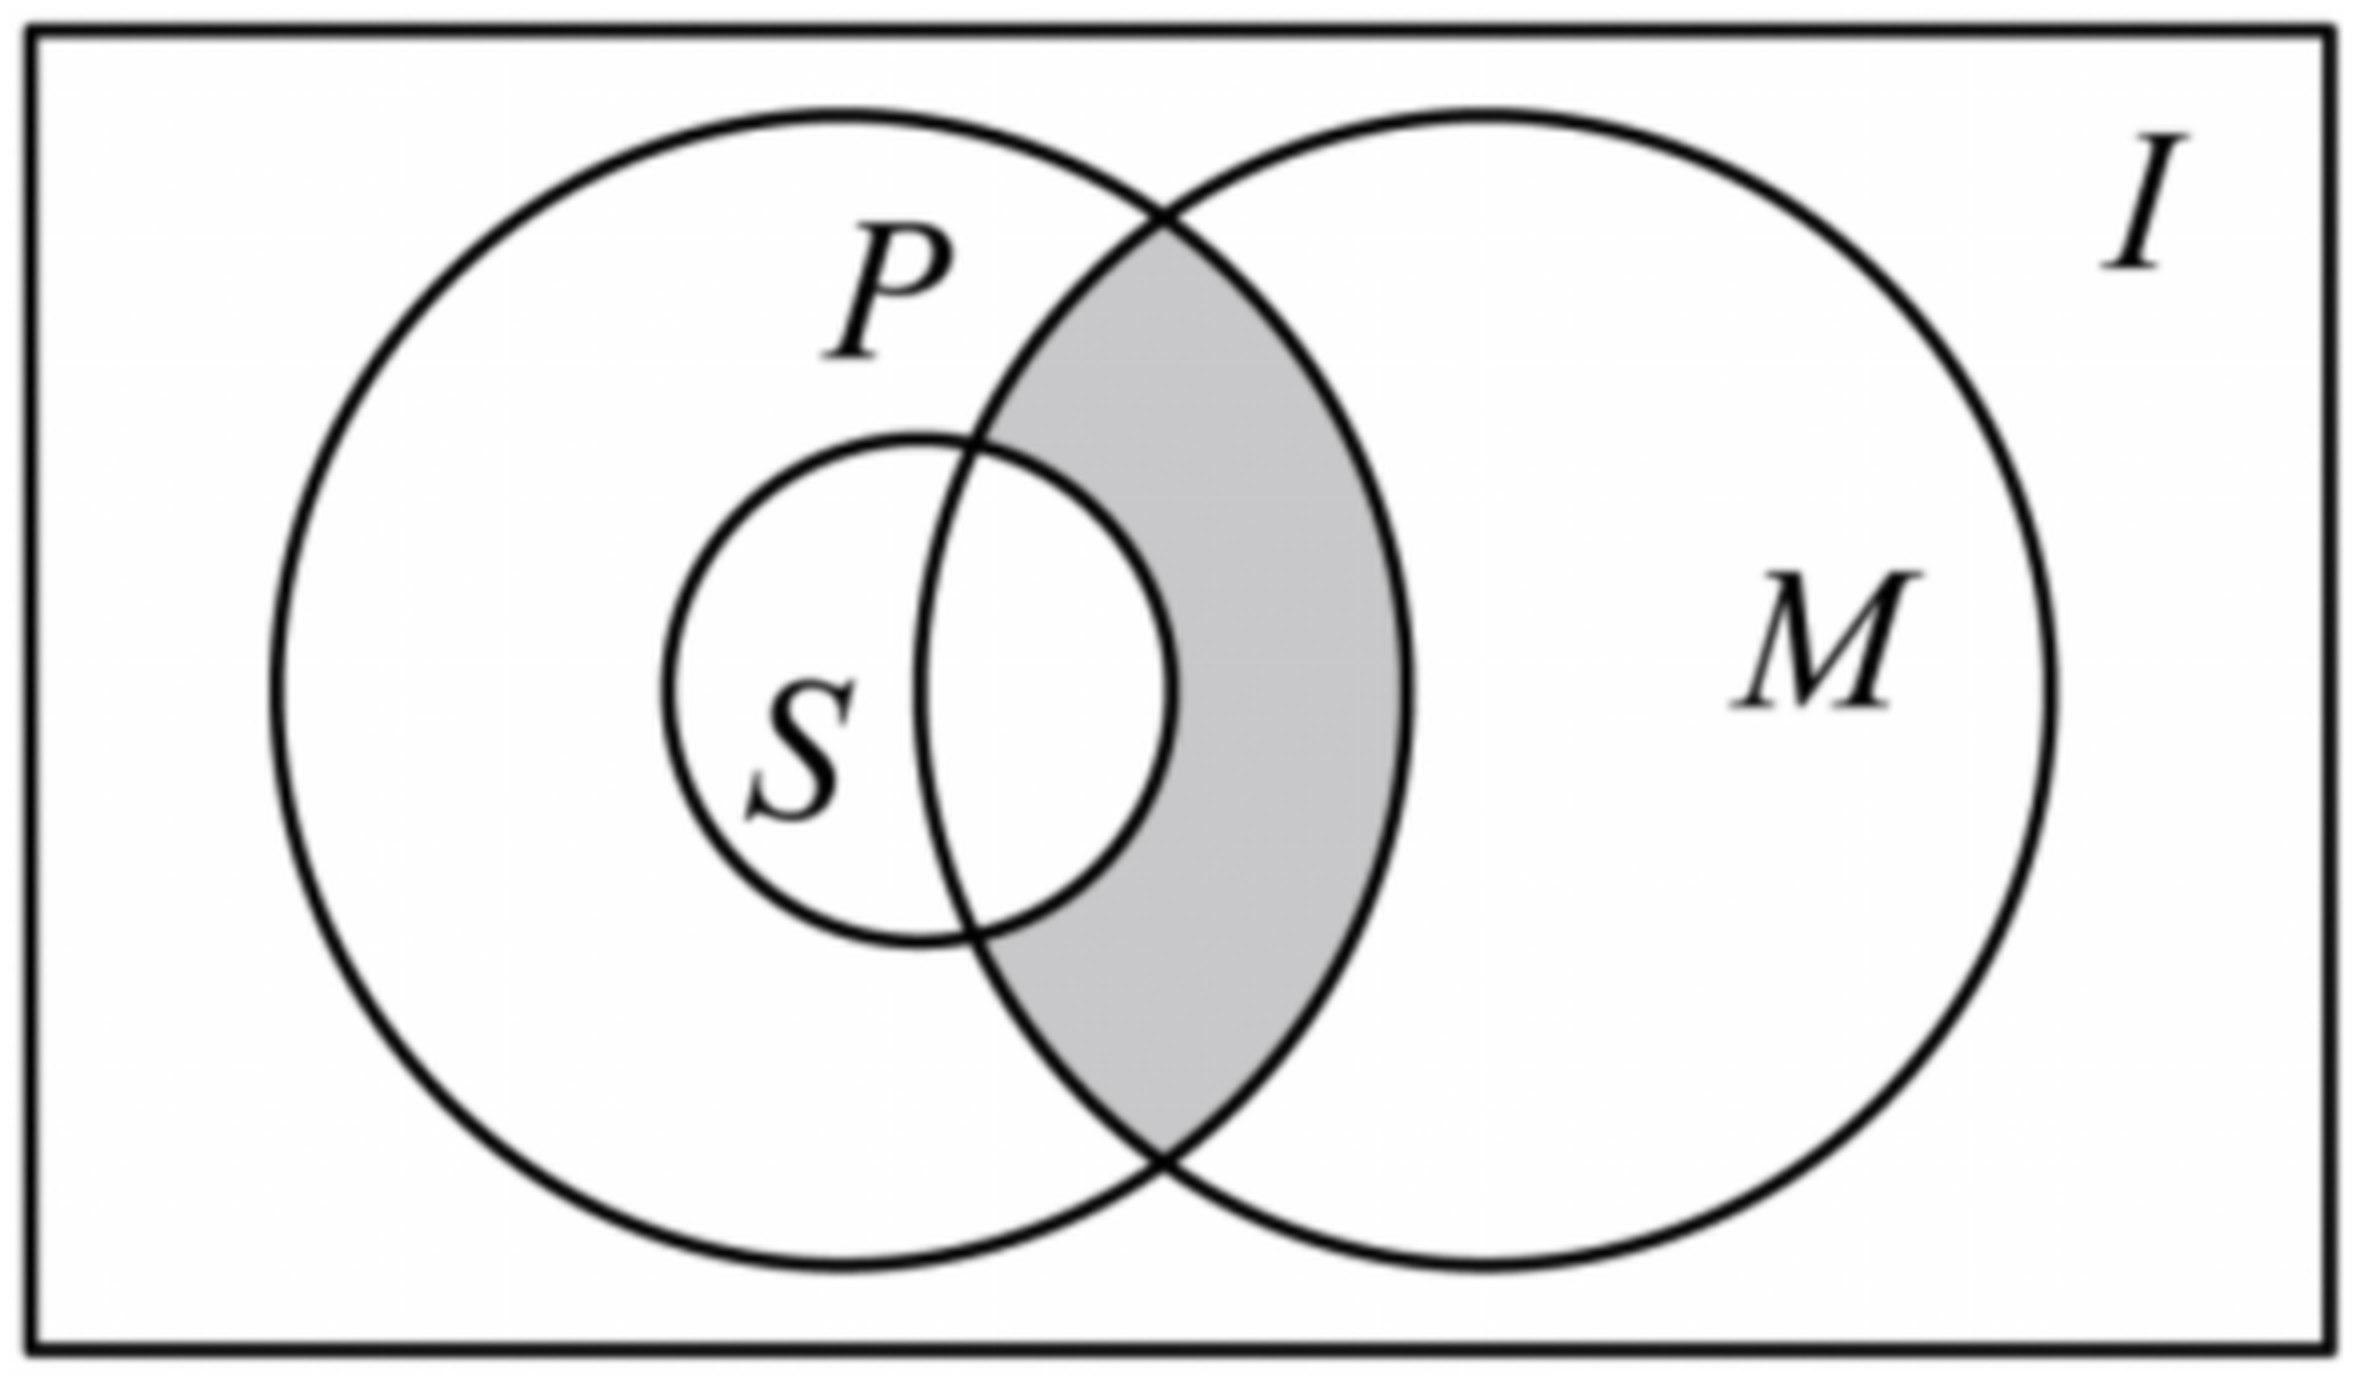
\includegraphics[width=0.46\textwidth]{figures/venn_MP_minus_S_h32.png}
\end{center}

\keepwithprev
A. $(M\cap P)\cap S$\qquad\qquad B. $(M\cap P)\cup S$

C. $(M\cap P)\cap\overline{S}$\qquad\qquad D. $(M\cap P)\cup\overline{S}$

\ans{$C$}

\ifanswer
\solbegin
\step{由 Venn 图得，集合表示 $M$、$P$ 的交集与 $S$ 的补集的交集，}
\step{即阴影部分所表示的集合是 $(M\cap P)\cap\overline{S}$. 故选 $C$.}
\solend

\fi

\item 若实数 $a$、$b$ 满足 $ab>0$，$a+2b=6$，则下列结论中错误的是\mbox{（\quad）}

\keepwithprev
A. $ab\leqslant\dfrac92$\qquad\qquad B. $a^2+4b^2\geqslant18$

C. $\dfrac1a+\dfrac2b$ 的最小值为 $\dfrac94$\qquad\qquad
D. $\dfrac{a^2}{a+1}+\dfrac{4b^2}{2b+1}$ 的最小值为 $\dfrac92$

\ans{$C$}

\ifanswer
\solbegin
\step{因为 $ab>0$，所以 $a$、$b$ 同号，又 $a+2b=6$，所以 $a$、$b$ 同正.}
\step{对于 $A$，由 $6=a+2b\geqslant2\sqrt{a\cdot2b}$ 得 $ab\leqslant\dfrac92$，故 $A$ 正确；}
\step{对于 $B$，由不等式 $\sqrt{\dfrac{m^2+n^2}2}\geqslant\dfrac{m+n}2$ 得
$\sqrt{\dfrac{a^2+(2b)^2}2}\geqslant\dfrac{a+2b}2=3$，}
\step{所以 $a^2+4b^2\geqslant18$，当且仅当 $a=2b=3$ 时取等号，故 $B$ 正确；}
\step{对于 $C$，$\dfrac1a+\dfrac2b
=\dfrac16\left(\dfrac1a+\dfrac2b\right)(a+2b)
=\dfrac16\left(5+\dfrac{2b}a+\dfrac{2a}b\right)$}
\step{$=\dfrac56+\dfrac13\left(\dfrac ba+\dfrac ab\right)
\geqslant\dfrac56+\dfrac13\times2\sqrt{\dfrac ba\cdot\dfrac ab}=\dfrac32$，}
\step{当且仅当 $\dfrac ba=\dfrac ab$，即 $a=b=2$ 时取等号，故 $C$ 错误；}
\step{对于 $D$，$\dfrac{a^2}{a+1}+\dfrac{4b^2}{2b+1}
=\dfrac{(a+1)^2-2(a+1)+1}{a+1}+\dfrac{(2b+1)^2-2(2b+1)+1}{2b+1}$}
\step{$=(a+1)-2+\dfrac1{a+1}+(2b+1)-2+\dfrac1{2b+1}
=(a+2b-2)+\dfrac1{a+1}+\dfrac1{2b+1}$}
\step{$=(6-2)+\dfrac{a+2b+2}{(a+1)(2b+1)}
=4+\dfrac8{(a+1)(2b+1)}$，}
\step{因为 $(a+1)(2b+1)\leqslant\left(\dfrac{a+1+2b+1}2\right)^2
=\left(\dfrac82\right)^2=16$，}
\step{当且仅当 $a+1=2b+1$，即 $a=2b=3$ 时取等号，}
\step{所以 $4+\dfrac8{(a+1)(2b+1)}\geqslant4+\dfrac8{16}=\dfrac92$，
故 $D$ 正确，其他几种方法同 12 题.}
\step{故选 $C$.}
\solend

\fi

% 注：本题的答案「D」原卷直接印在题干末尾的括号内，本稿按全稿惯例另提为 \ans{}。
\item 已知函数 $f(x)=x^2-2ax+a^2-1$，定义集合 $A=\{x\mid f(x)<0\}$. 若集合
$\{x\mid f(x)\in A\}=\varnothing$，则实数 $a$ 的取值范围是\mbox{（\quad）}

\keepwithprev
A. $(-3,-2)$\qquad B. $[-3,-2]$\qquad
C. $(-\infty,2)$\qquad D. $(-\infty,-2]$

\ans{$D$}

\item 非空集合 $A$ 具有如下性质：①若 $x$、$y\in A$，则 $\dfrac xy\in A$；
②若 $x$、$y\in A$，则 $x+y\in A$；

由此可知：下列判断中，错误的是\mbox{（\quad）}

\keepwithprev
A. $-1\notin A$\qquad\qquad B. $\dfrac{2025}{2026}\in A$

C. 若 $x$、$y\in A$，则 $xy\in A$\qquad\qquad
D. 若 $x$、$y\in A$，则 $x-y\in A$

\ans{$D$}

\ifanswer
\solbegin
\step{由题意得 $0\notin A$，$1\in A$，}
\step{对于 $A$，假设 $-1\in A$，则 $-1+1=0\in A$，矛盾，所以 $-1\notin A$，故 $A$ 正确；}
\step{对于 $B$，由 $1\in A$，得 $1+1=2\in A$，$2+1=3\in A$，…，$2025\in A$，$2026\in A$，}
\step{所以 $\dfrac{2025}{2026}\in A$，故 $B$ 正确；}
\step{对于 $C$，因为 $1\in A$，$x\in A$，所以 $\dfrac1x\in A$，
又因为 $y\in A$，所以 $\dfrac y{\frac1x}=xy\in A$，}
\step{故 $C$ 正确；}
\step{对于 $D$，因为 $1\in A$，$2\in A$，若 $x=1$，$y=2$，则 $x-y=-1\notin A$，故 $D$ 错误.}
\step{故选 $D$.}
\solend

\fi

\end{enumerate}

\bigsec{三、解答题}

\begin{enumerate}
\setcounter{enumi}{16}

\item 求下列关于实数 $x$ 的不等式的解集.

\begin{enumerate}[label=(\arabic*)]
\item $|2x+1|<5x-1$；
\item $\dfrac{(x-1)(x-3)(x-6)}{(x-2)(x-4)^2(x-5)}\geqslant0$.
\end{enumerate}

\ifanswer
\solbegin
\stepm{(1)}{因为不等式 $|2x+1|<5x-1$ 可化为 $-(5x-1)<2x+1<5x-1$，且 $5x-1>0$，}
\step{解得 $x>\dfrac23$，所以原不等式的解集为 $\left(\dfrac23,+\infty\right)$；}
\stepm{(2)}{不等式 $\dfrac{(x-1)(x-3)(x-6)}{(x-2)(x-4)^2(x-5)}\geqslant0$，}
\step{等价于 $(x-1)(x-3)(x-6)(x-2)(x-5)\geqslant0$，
且 $x-2\neq0$，$x-4\neq0$，$x-5\neq0$，}
\step{由“穿针引线法”，解得 $1\leqslant x<2$ 或 $3\leqslant x<4$ 或 $4<x<5$ 或 $x\geqslant6$，}
\step{所以不等式的解集为 $[1,2)\cup[3,4)\cup(4,5)\cup[6,+\infty)$.}
\solend

\fi

\ansspace[6]

\item 已知集合 $A=\left\{x\left|mx^2-mx+\dfrac{5m}2-6=0\right.\right\}\neq\varnothing$，
集合 $B=\{x\mid1<x<4$ 且 $x\in\Z\}$，$C=\{x\mid ax+3>0\}$；若 $A\cap B=A$.

\begin{enumerate}[label=(\arabic*)]
\item 求 $m$ 的取值范围.
\item 设 $m$ 的取值集合为 $D$，若 $C\cap D=\varnothing$，求 $m$ 的值及其对应 $a$ 的取值范围.
\end{enumerate}

\ans{略}

\ansspace[8]

\item 已知函数 $f(x)=x^2+(m-2)x+2m-1$.

\begin{enumerate}[label=(\arabic*)]
\item 若 $f(x)=0$ 的两根为 $x_1$、$x_2$，且 $|x_1-x_2|=2$，求实数 $m$ 的值；
\item 若函数 $y=f(x)$ 的图像在区间 $(0,1)$ 上与 $x$ 轴只有一个交点，
求实数 $m$ 的取值范围.
\end{enumerate}

\ifanswer
\solbegin
\stepm{(1)}{由题意得 $x_1+x_2=-(m-2)=2-m$，$x_1x_2=2m-1$，}
\step{由 $|x_1-x_2|=\sqrt{(x_1+x_2)^2-4x_1x_2}
=\sqrt{(2-m)^2-4(2m-1)}=2$，}
\step{化简得 $m^2-12m+4=0$，解得 $m=6\pm4\sqrt2$，故 $m=6\pm4\sqrt2$.}
\stepm{(2)}{当 $f(x)=0$ 只有一个根，且此根位于区间 $(0,1)$，}
\step{则 $\begin{cases}0<\dfrac{2-m}2<1\\[4pt]
\Delta=(m-2)^2-4(2m-1)=0\end{cases}$，
解得 $\begin{cases}0<m<2\\ m=6-2\sqrt7\text{ 或 }m=6+2\sqrt7\end{cases}$，}
\step{所以 $m=6-2\sqrt7$；}
\step{当 $f(x)=0$ 有两个根时，有一个根在区间 $(0,1)$ 内，且另一个根位于 $[0,1]$ 之外，}
\step{则 $\begin{cases}f(0)f(1)<0\\ \Delta=(m-2)^2-4(2m-1)>0\end{cases}$，
解得 $\begin{cases}\dfrac12<m<\dfrac23\\[4pt]
m<6-2\sqrt7\text{ 或 }m>6+2\sqrt7\end{cases}$，}
% 注：下一行原卷作「即 $\dfrac12<m<\dfrac32$」，按上一行方程组应为
%     $\dfrac12<m<\dfrac23$（同页最终答案也印证），照录未改，见文件头「原卷存疑」①。
\step{即 $\dfrac12<m<\dfrac32$；}
\step{当 $f(x)=0$ 有两个根位于区间 $[0,1]$ 内，且只有一个根在区间 $(0,1)$ 内，}
\step{则另一个根为 $0$ 时，得 $m=\dfrac12$，此时 $x_1+x_2=\dfrac32$，
解得另一个根 $x_2=\dfrac32>0$，故此种情况不符题意；}
\step{当 $f(x)=0$ 有两个根位于区间 $(0,1]$ 内，且只有一个根在区间 $(0,1)$ 内，}
\step{则另一个根为 $1$ 时，得 $m=\dfrac23$，此时 $x_1+x_2=\dfrac43$，
解得另一个根 $x_2=\dfrac13$，故此种情况符合题意；}
\step{综上所述，$m$ 的取值范围为
$\left(\dfrac12,\dfrac23\right]\cup\{6-2\sqrt7\}$.}
\solend

\fi

\ansspace[8]

\item 设集合 $A=\{a_1,a_2,a_3,a_4\}$，$B=\{b_1,b_2,b_3,b_4\}$，$C=\{2,3,4,6\}$，
新定义：集合 $A$ 中所有含 $k$ 个元素的子集中 $k$ 个元素之和组成的集合为“$k$ 元集和集”，
集合 $A$ 中所有含 $k$ 个元素的子集中最大元素减去剩余所有元素的和组成的集合为“$k$ 元差集”.

\begin{enumerate}[label=(\arabic*)]
\item 若 $A$ 的“$k$ 元集和集”为 $C$，求：集合 $A$.
\item 在 (1) 的条件下，若 $B$ 的“$k$ 元差集”为 $C$，求：所有满足条件的 $A\cap B$ 的真子集
个数之和.
\item 设 $b_1=a_1^2$，$b_2=a_2^2$，$b_3=a_3^2$，$b_4=a_4^2$，若 $A\cap B$ 为 $2$ 元集且
元素之和为 $10$ 且 $A$ 的“$2$ 元集和集”中最大元素不超过 $14$，求：所有满足条件的 $A$ 的
“$3$ 元差集”.
\end{enumerate}

\ifanswer
\solbegin
\stepm{(1)}{若 $A$ 的“$k$ 元集和集”为 $C$，$C=\{2,3,4,6\}$，则集合为 $\{-1,1,2,3\}$；}
\stepm{(2)}{$B$ 集合为 $\{5,3,0,-1\}$ 或 $\{9,3,1,0\}$ 或 $\{6,3,1,-1\}$，}
\step{故所有 $A\cap B$ 的真子集个数之和为 $13$；}
\stepm{(3)}{$b_1=a_1^2$，$b_2=a_2^2$，$b_3=a_3^2$，$b_4=a_4^2$，}
\step{若 $A\cap B$ 为 $2$ 元集且元素之和为 $10$，
且 $A$ 的“$2$ 元集和集”中最大元素不超过 $14$，}
% 注：下一行答案的第二个集合 $\{0,4,5,6\}$ 是 4 元集，而题问的却是「3 元差集」，
%     原卷如此，照录未改，见文件头「原卷存疑」③。
\step{则满足条件的 $A$ 的“$3$ 元差集” $\{1,3,5\}$ 或 $\{0,4,5,6\}$ 或 $\{2,4,5,8\}$.}
\solend

\fi

\ansspace[8]

\item 已知有限集 $X$、$Y$，定义集合 $X-Y=\{x\mid x\in X$ 且 $x\notin Y\}$，
$|X|$ 表示集合 $X$ 元素个数.

\begin{enumerate}[label=(\arabic*)]
\item 若 $X=\{1,2,3,4\}$，$Y=\{3,4,5\}$，写出集合 $X-Y$ 和 $Y-X$，以及
$|(X-Y)\cup(Y-X)|$ 的值；
\item 给定正整数 $n$，集合 $S=\{1,2,\cdots,n\}$，对于实数集的非空有限子集 $A$、$B$，
定义集合 $C=\{x\mid x=a+b,a\in A,b\in B\}$；

①求证：$|A-S|+|B-S|+|S-C|\geqslant1$；

②求 $|(A-S)\cup(S-A)|+|(B-S)\cup(S-B)|+|(C-S)\cup(S-C)|$ 的最小值.
\end{enumerate}

\ifanswer
\solbegin
\stepm{(1)}{由定义直接得 $X-Y=\{1,2\}$，$Y-X=\{5\}$，
$|(X-Y)\cup(Y-X)|=3$.}
% 注：下一句原卷作「显然 $|X|\geqslant0$」（按后文论证疑为 $|S|\geqslant0$），
%     照录未改，见文件头「原卷存疑」②。
\stepm{(2)}{①显然 $|X|\geqslant0$.}
\step{若 $A\cup B$ 中含有一个不在 $S$ 中的元素，则 $|A-S|+|B-S|\geqslant1$，
即 $|A-S|+|B-S|+|S-C|\geqslant1$.}
\step{若 $A\sub S$，且 $B\sub S$，则 $|A-S|=|B-S|=0$；}
\step{此时 $A$ 中最小的元素 $a\geqslant1$，$B$ 中最小的元素 $b\geqslant1$，
所以 $C$ 中最小的元素 $a+b\geqslant2$，所以 $1\notin C$.}
\step{因为 $S=\{1,2,\cdots,n\}$，所以 $|S-C|\geqslant1$，
即 $|A-S|+|B-S|+|S-C|\geqslant1$.}
\step{综上，$|A-S|+|B-S|+|S-C|\geqslant1$.}
\step{②由①得 $|A-S|+|B-S|+|S-C|\geqslant1$.}
\step{所以 $|(A-S)\cup(S-A)|+|(B-S)\cup(S-B)|+|(C-S)\cup(S-C)|$}
\step{$=|A-S|+|S-A|+|B-S|+|S-B|+|C-S|+|S-C|$}
\step{$\geqslant|S-A|+|S-B|+|C-S|+1$.}
\step{若 $A\cap S=\varnothing$，或 $B\cap S=\varnothing$，则 $|S-A|+|S-B|\geqslant n$.}
\step{若 $A\cap S\neq\varnothing$，且 $B\cap S\neq\varnothing$，
设 $A\cap S=\{a_1,a_2,\cdots,a_s\}$，$B\cap S=\{b_1,b_2,\cdots,b_t\}$，}
\step{且 $1\leqslant a_1<a_2<\cdots<a_s\leqslant n$，
$1\leqslant b_1<b_2<\cdots<b_t\leqslant n$，则 $|S-A|=n-s$，$|B-S|=n-t$.}
% 注：原卷的解析到此为止（第 10 页末），②的最小值并未给出，照录未补，
%     见文件头「原卷存疑」④。
\solend

\fi

\ansspace*[10]

\end{enumerate}

\end{document}
"
% 紧凑版：xelatex "\def\iscompact{1}% 高一32_华师大二附中_周末作业4.tex
%   —— 高一上数学「2026-2027 年华师大二附中高一上周末作业 4」（试卷版/答案版）
% 试卷版：xelatex 高一32_华师大二附中_周末作业4.tex
% 答案版：xelatex "\def\isanswer{1}\input{高一32_华师大二附中_周末作业4.tex}"
% 紧凑版：xelatex "\def\iscompact{1}\input{高一32_华师大二附中_周末作业4.tex}"
%
% 原始材料是微信公众号图文（公众号「魔都数学加油站」连载「27学年高一 32」，2026-09-25 发布，
% 原文标题「27学年高一32——2026-2027年上海市华师大二附中高一上周末作业4」），
% 正文为 10 张 PNG 页。**同一篇里各页分辨率不一致**（2560×3620 与 4762×6735 两档混排），
% 取 mmbiz.qpic.cn/<hash>/0 的原图档。原文本身就是一份**讲评版**——有的题下方印【解析】、
% 有的印【答案】，第 15 题的答案直接印在题干末尾的括号里。
% 试题文字、答案与解析均照原卷录入，未改内容。卷面的粉色斜水印属水印，未录入。
%
% ⚠ 卷首年份：本卷卷面印作「**2025-2026 年**」，与连载「27学年高一32」及公众号原文标题的
%   「2026-2027 年」**不一致**。经三人次分别把标题行裁出放大（4×—10×）独立判读，三次都读作
%   2025-2026，且校名作「华师大二附中」（无「东」字）、卷面亦无「上海市」三字。
%   按全稿「标题行照原卷」的口径，本稿照卷面排作「2025--2026 年…」——这是全稿唯一一份
%   年份不是 2026--2027 的卷子（其余 35 份均为 2026--2027）。
%
% 卷首标题：原卷印作「……年华师大二附中高一上周末作业 4」（公众号标题里的「上海市」
% 三字卷面标题行没有，本稿照卷面），年份区间按全稿惯例排 en dash，前缀照原卷保留「年」。
%
% 与原卷的排版差异（均已在 README「说明」中交代）：
%   ① 原文自**第 3 题**起（第 1、2 题未在该文中发布），故本稿题号亦自 3 起；
%   ② 原卷本就印有「一、填空题」「二、选择题」「三、解答题」三节标题，本稿照原卷分节，
%      只把标题改排成全稿统一的「大节标题」样式；
%   ③ 原卷第 6、8、9 题只印【答案】行（第 18 题的【答案】印作「略”），其余各题印【解析】，
%      第 15 题的答案直接印在题干末尾的括号内；本稿统一改为试卷版隐去、
%      答案版以 \ans{}／\ifanswer 块给出，两版彻底分离；
%   ④ 子集符号原卷两种并用：第 21(2)① 的 $A\sub S$、$B\sub S$ 带下划线，
%      第 3、10 题的 $(0,2)\subset(-\infty,3)$、$A\subset B$、$\overline{B}\subset\overline{A}$
%      作真包含，本稿分别照录为 $\sub$ 与 $\subset$；
%   ⑤ 补集符号原卷一律作上横线（$\overline{A}$、$\overline{B}$、$\overline{S}$），本稿照录；
%      空集原卷作「斜杠伸出圆外」的 $\varnothing$；
%   ⑥ 判别式记号原卷两种：第 4 题作粗体的 $\Delta$、第 11 题作细等宽的 $\triangle$，本稿照录；
%   ⑦ 数集记号原卷作斜体的 $R$、$Z$（第 4、18 题），本稿按全稿惯例统一写作 $\R$、$\Z$；
%   ⑧ 原卷填空的横线约两个字宽，本稿按全稿惯例统一排 \blankline[4.4em]；
%   ⑨ 原卷未印副标题，本稿按全稿惯例补出副标题「集合与常用逻辑用语」；
%   ⑩ 本卷只有第 13 题一图（韦恩图），原卷印在题干右侧，本稿移至题干之后；
%      图取原卷截图、4× LANCZOS 放大（figures/venn_MP_minus_S_h32.png）。
%
% 原卷存疑四处（均照抄原卷、未改，见源码中该处上方注释）：
%   ① 第 19(2)【解析】有「即 $\dfrac12<m<\dfrac32$」，按上一行的方程组应为
%      $\dfrac12<m<\dfrac23$（同页最终答案 $\left(\dfrac12,\dfrac23\right]$ 也印证）；
%   ② 第 21(2)① 首句作「显然 $|X|\geqslant0$」（按后文论证疑为 $|S|\geqslant0$）；
%   ③ 第 20(3) 的答案第二个集合 $\{0,4,5,6\}$ 是 4 元集，而题问的是「3 元差集」；
%   ④ 第 21(2)② 的解析**原卷就未写完**（第 10 页到「则 $|S-A|=n-s$，$|B-S|=n-t$」即止）。

\documentclass[a4paper,11pt]{article}
\usepackage{common}

\begin{document}

\examtitlest[3]{2025--2026 年华师大二附中高一上周末作业 4}{集合与常用逻辑用语}

\bigsec{一、填空题}

\begin{enumerate}
\setcounter{enumi}{2}

\item 设 $x$ 为实数，则“$x<3$”是“$x(x-2)<0$”的 \blankline[4.4em] 条件.

\ifanswer
\solbegin
\step{$x(x-2)<0$，解得 $0<x<2$，$(0,2)\subset(-\infty,3)$，}
\step{若 $x$ 属于“$x(x-2)<0$”，则属于“$x<3$”一定成立，即满足必要性，}
\step{若 $x$ 属于“$x<3$”，不一定满足“$x(x-2)<0$”，如 $x=-1$，即充分性不成立；}
\step{故“$x<3$”是“$x(x-2)<0$”的必要不充分条件.}
\solend

\fi

\item 若关于 $x$ 的不等式 $kx^2-kx+1>0$ 的解集为 $\R$，则实数 $k$ 的取值范围为
\blankline[4.4em].

\ifanswer
\solbegin
\step{①当 $k=0$ 时，不等式为 $1>0$ 恒成立，满足题意；}
\step{②当 $k\neq0$ 时，只要 $\begin{cases}k>0\\ \Delta=k^2-4k<0\end{cases}$，
解得 $0<k<4$；}
\step{所以不等式 $kx^2-kx+1>0$ 的解集为 $\R$，则实数 $k$ 的取值范围为 $[0,4)$.}
\solend

\fi

\item 已知 $1<a<3$，$-5<b<-2$，则 $\dfrac ab$ 的取值范围是 \blankline[4.4em].

\ifanswer
\solbegin
\step{因为 $-5<b<-2$，所以 $2<-b<5$，$\dfrac15<-\dfrac1b<\dfrac12$，又 $1<a<3$，}
\step{得 $\dfrac15<-\dfrac ab<\dfrac32$，则 $-\dfrac32<\dfrac ab<-\dfrac15$，
故 $\dfrac ab$ 的取值范围是 $\left(-\dfrac32,-\dfrac15\right)$.}
\solend

\fi

\item 关于 $x$ 的不等式 $\dfrac{ax-1}{x-a}>1$ 的解集为 $A$，且 $3\notin A$，
则实数 $a$ 的取值范围为 \blankline[4.4em].

\ans{$(-\infty,1]\cup[3,+\infty)$}

\item 若关于 $x$ 的不等式 $a\leqslant\dfrac34x^2-3x+4\leqslant b$ 的解集恰好是 $[a,b]$，
则 $b-a=$ \blankline[4.4em].

\ifanswer
\solbegin
\step{令 $f(x)=\dfrac34x^2-3x+4$，则 $f(x)$ 的对称轴为 $x=2$，}
\step{画出函数 $f(x)=\dfrac34x^2-3x+4=\dfrac34(x-2)^2+1$ 的图象，
得 $f(x)_{\min}=f(2)=1$，}
\step{由题意得 $a\leqslant1$，且 $f(a)=f(b)=b$，$a<b$，}
\step{由 $f(b)=b$ 得 $\dfrac34b^2-3b+4=b$，解得 $b=\dfrac43$（舍去）或 $b=4$，得 $b=4$，}
\step{由抛物线的对称轴为 $x=2$ 得 $a=0$，所以 $b-a=4$.}
\solend

\fi

\item 若关于 $x$ 的方程 $x^2-2kx+k+4=0$ 在 $[1,2]$ 上有解，则实数 $k$ 的取值范围为
\blankline[4.4em].

\ans{$\left[\dfrac83,5\right]$}

\item 记关于 $x$ 的方程 $x^2-2mx-2m+3=0$ 的两实根为 $x_1$、$x_2$，
则 $(x_1-2)^2+(x_2-2)^2$ 的最小值为 \blankline[4.4em].

\ans{$2$}

\item 若“$|mx^2-4x+3|\geqslant2$”的必要非充分条件是“$x\leqslant1$ 或 $x\geqslant4$”，
则实数 $m$ 的取值范围是 \blankline[4.4em].

\ifanswer
\solbegin
\step{记 $|mx^2-4x+3|\geqslant2$ 的解集为集合 $A$，
$B=\{x\mid x\leqslant1\text{ 或 }x\geqslant4\}$，}
\step{则 $\overline{A}$ 为 $|mx^2-4x+3|<2$ 的解集，$\overline{B}=\{x\mid1<x<4\}$；}
\step{因为 $B$ 是 $A$ 的必要非充分条件，所以 $A\subset B$，
得 $\overline{B}\subset\overline{A}$，}
\step{即对任意 $x\in(1,4)$，都有 $|mx^2-4x+3|<2$ 恒成立.}
\step{因为 $|mx^2-4x+3|<2$，$1<x<4$，所以 $-2<mx^2-4x+3<2$，}
\step{化简得
$-5\left(\dfrac1x\right)^2+4\left(\dfrac1x\right)
<m<-\left(\dfrac1x\right)^2+4\left(\dfrac1x\right)$；}
\step{令 $t=\dfrac1x$，$g(t)=-5t^2+4t$，$h(t)=-t^2+4t$，
且 $t\in\left(\dfrac14,1\right)$；}
\step{所以 $g(t)=-5t^2+4t=-5\left(t-\dfrac25\right)^2+\dfrac45$，
当 $t=\dfrac25$ 时，$g(t)$ 取得最大值 $\dfrac45$，}
\step{$h(t)=-t^2+4t=-(t-2)^2+4$，当 $t=\dfrac14$ 时，$h(t)$ 取得最小值，
即 $h(t)>h\left(\dfrac14\right)=\dfrac{15}{16}$；}
\step{因为对任意 $t\in\left(\dfrac14,1\right)$，$g(t)<m<h(t)$ 恒成立，
所以 $g\left(\dfrac25\right)<m\leqslant h\left(\dfrac14\right)$，}
\step{即 $\dfrac45<m\leqslant\dfrac{15}{16}$，
所以 $m$ 的取值范围是 $\left(\dfrac45,\dfrac{15}{16}\right]$.}
\solend

\fi

\item 已知关于 $x$ 的方程 $x^2+2(m-2)x+m^2-3m+3=0$ 有两个不相等的实数根 $x_1$、$x_2$，则

$\dfrac{mx_1}{x_1-1}+\dfrac{mx_2}{x_2-1}-\dfrac2{x_1+x_2-2}$ 的最大值为 \blankline[4.4em].

\ifanswer
\solbegin
\step{关于 $x$ 的方程 $x^2+2(m-2)x+m^2-3m+3=0$ 有两个不相等的实数根 $x_1$、$x_2$，}
\step{则 $\triangle=4(m-2)^2-4(m^2-3m+3)=-4m+4>0$，得 $m<1$，}
\step{且 $x_1+x_2=-2(m-2)$，$x_1x_2=m^2-3m+3$，}
\step{$\dfrac{mx_1}{x_1-1}+\dfrac{mx_2}{x_2-1}-\dfrac2{x_1+x_2-2}
=\dfrac{m[2x_1x_2-(x_1+x_2)]}{x_1x_2-(x_1+x_2)+1}+\dfrac1{m-1}$}
\step{$=\dfrac{2m(m-1)^2}{m^2-m}+\dfrac1{m-1}=2(m-1)+\dfrac1{m-1}$，}
\step{又因为 $m<1$，所以 $m-1<0$，则 $1-m>0$，}
\step{所以 $2(1-m)+\dfrac1{1-m}\geqslant2\sqrt{2(1-m)\cdot\dfrac1{1-m}}=2\sqrt2$，}
\step{当且仅当 $2(1-m)=\dfrac1{1-m}$ 时，即 $m=1-\dfrac{\sqrt2}2$ 时取等号，}
\step{所以 $2(m-1)+\dfrac1{m-1}\leqslant-2\sqrt2$，
即 $\dfrac{mx_1}{x_1-1}+\dfrac{mx_2}{x_2-1}-\dfrac2{x_1+x_2-2}$ 的最大值为 $-2\sqrt2$.}
\solend

\fi

\item 若正实数 $a$、$b$ 满足 $a+2b=ab$，则 $\dfrac4{a^2+2a}+\dfrac1{2b^2+b}$ 的最小值是
\blankline[4.4em].

\ifanswer
\solbegin
\stepm{法一}{由 $a+2b=ab$，得 $\dfrac2a+\dfrac1b=1$，}
\step{令 $x=\dfrac1a$，$y=\dfrac1b$，则 $x$、$y>0$，$2x+y=1$，$2x+1+y+2=4$，}
\step{所以 $\dfrac4{a^2+2a}+\dfrac1{2b^2+b}
=\dfrac4{\frac1{x^2}+\frac2x}+\dfrac1{\frac2{y^2}+\frac1y}
=\dfrac{4x^2}{2x+1}+\dfrac{y^2}{y+2}$（*）}
\step{$=\dfrac{(2x+1)^2-2(2x+1)+1}{2x+1}+\dfrac{(y+2)^2-4(y+2)+4}{y+2}$}
\step{$=2x-1+\dfrac1{2x+1}+y-2+\dfrac4{y+2}=\dfrac1{2x+1}+\dfrac4{y+2}-2$}
\step{$=\dfrac14\left(\dfrac1{2x+1}+\dfrac4{y+2}\right)(2x+1+y+2)-2$}
\step{$=\dfrac14\left[5+\dfrac{y+2}{2x+1}+\dfrac{4(2x+1)}{y+2}\right]-2
\geqslant\dfrac14(5+2\sqrt4)-2=\dfrac14$，}
\step{当且仅当 $\dfrac{y+2}{2x+1}=\dfrac{4(2x+1)}{y+2}$，
即 $x=\dfrac16$，$y=\dfrac23$ 时取等号，}
\step{故 $\dfrac4{a^2+2a}+\dfrac1{2b^2+b}$ 的最小值是 $\dfrac14$.}
\stepm{法二}{在法一（*）后，由权方和不等式，得
$\dfrac4{a^2+2a}+\dfrac1{2b^2+b}
=\dfrac{4x^2}{2x+1}+\dfrac{y^2}{y+2}
\geqslant\dfrac{(2x+y)^2}{2x+1+y+2}=\dfrac14$，}
\step{当且仅当……，故 $\dfrac4{a^2+2a}+\dfrac1{2b^2+b}$ 的最小值是 $\dfrac14$.}
\stepm{法三}{注意到
$\left(\dfrac{a+2}a+\dfrac{2b+1}b\right)\left(\dfrac4{a^2+2a}+\dfrac1{2b^2+b}\right)$}
\step{$\geqslant
\left(\sqrt{\dfrac{a+2}a\cdot\dfrac4{a^2+2a}}
+\sqrt{\dfrac{2b+1}b\cdot\dfrac1{2b^2+b}}\right)^2
=\left(\dfrac2a+\dfrac1b\right)^2$，}
\step{其中 $\dfrac{a+2}a+\dfrac{2b+1}b=3+\dfrac{a+2b}{ab}=4$，
$\dfrac2a+\dfrac1b=\dfrac{a+2b}{ab}=1$，}
\step{所以 $\dfrac4{a^2+2a}+\dfrac1{2b^2+b}\geqslant\dfrac14$，
当且仅当……，故 $\dfrac4{a^2+2a}+\dfrac1{2b^2+b}$ 的最小值是 $\dfrac14$.}
\solend

\fi

\end{enumerate}

\bigsec{二、选择题}

\begin{enumerate}
\setcounter{enumi}{12}

\item 如图，$I$ 为全集，$M$、$P$、$S$ 是 $I$ 的三个子集，则阴影部分所表示的集合是
\mbox{（\quad）}

\begin{center}
% 图取原卷截图、4× LANCZOS 放大（原卷把图印在题干右侧，本稿移至此处，见文件头⑩）。
% 矩形为全集 $I$，左大圆 $P$（内下方含小圆 $S$，其右侧伸入 $P$ 与 $M$ 的重叠区）、
% 右大圆 $M$；阴影是 $P$、$M$ 重叠的透镜形区域挖掉 $S$ 后剩下的部分（左缘呈弯月形）。
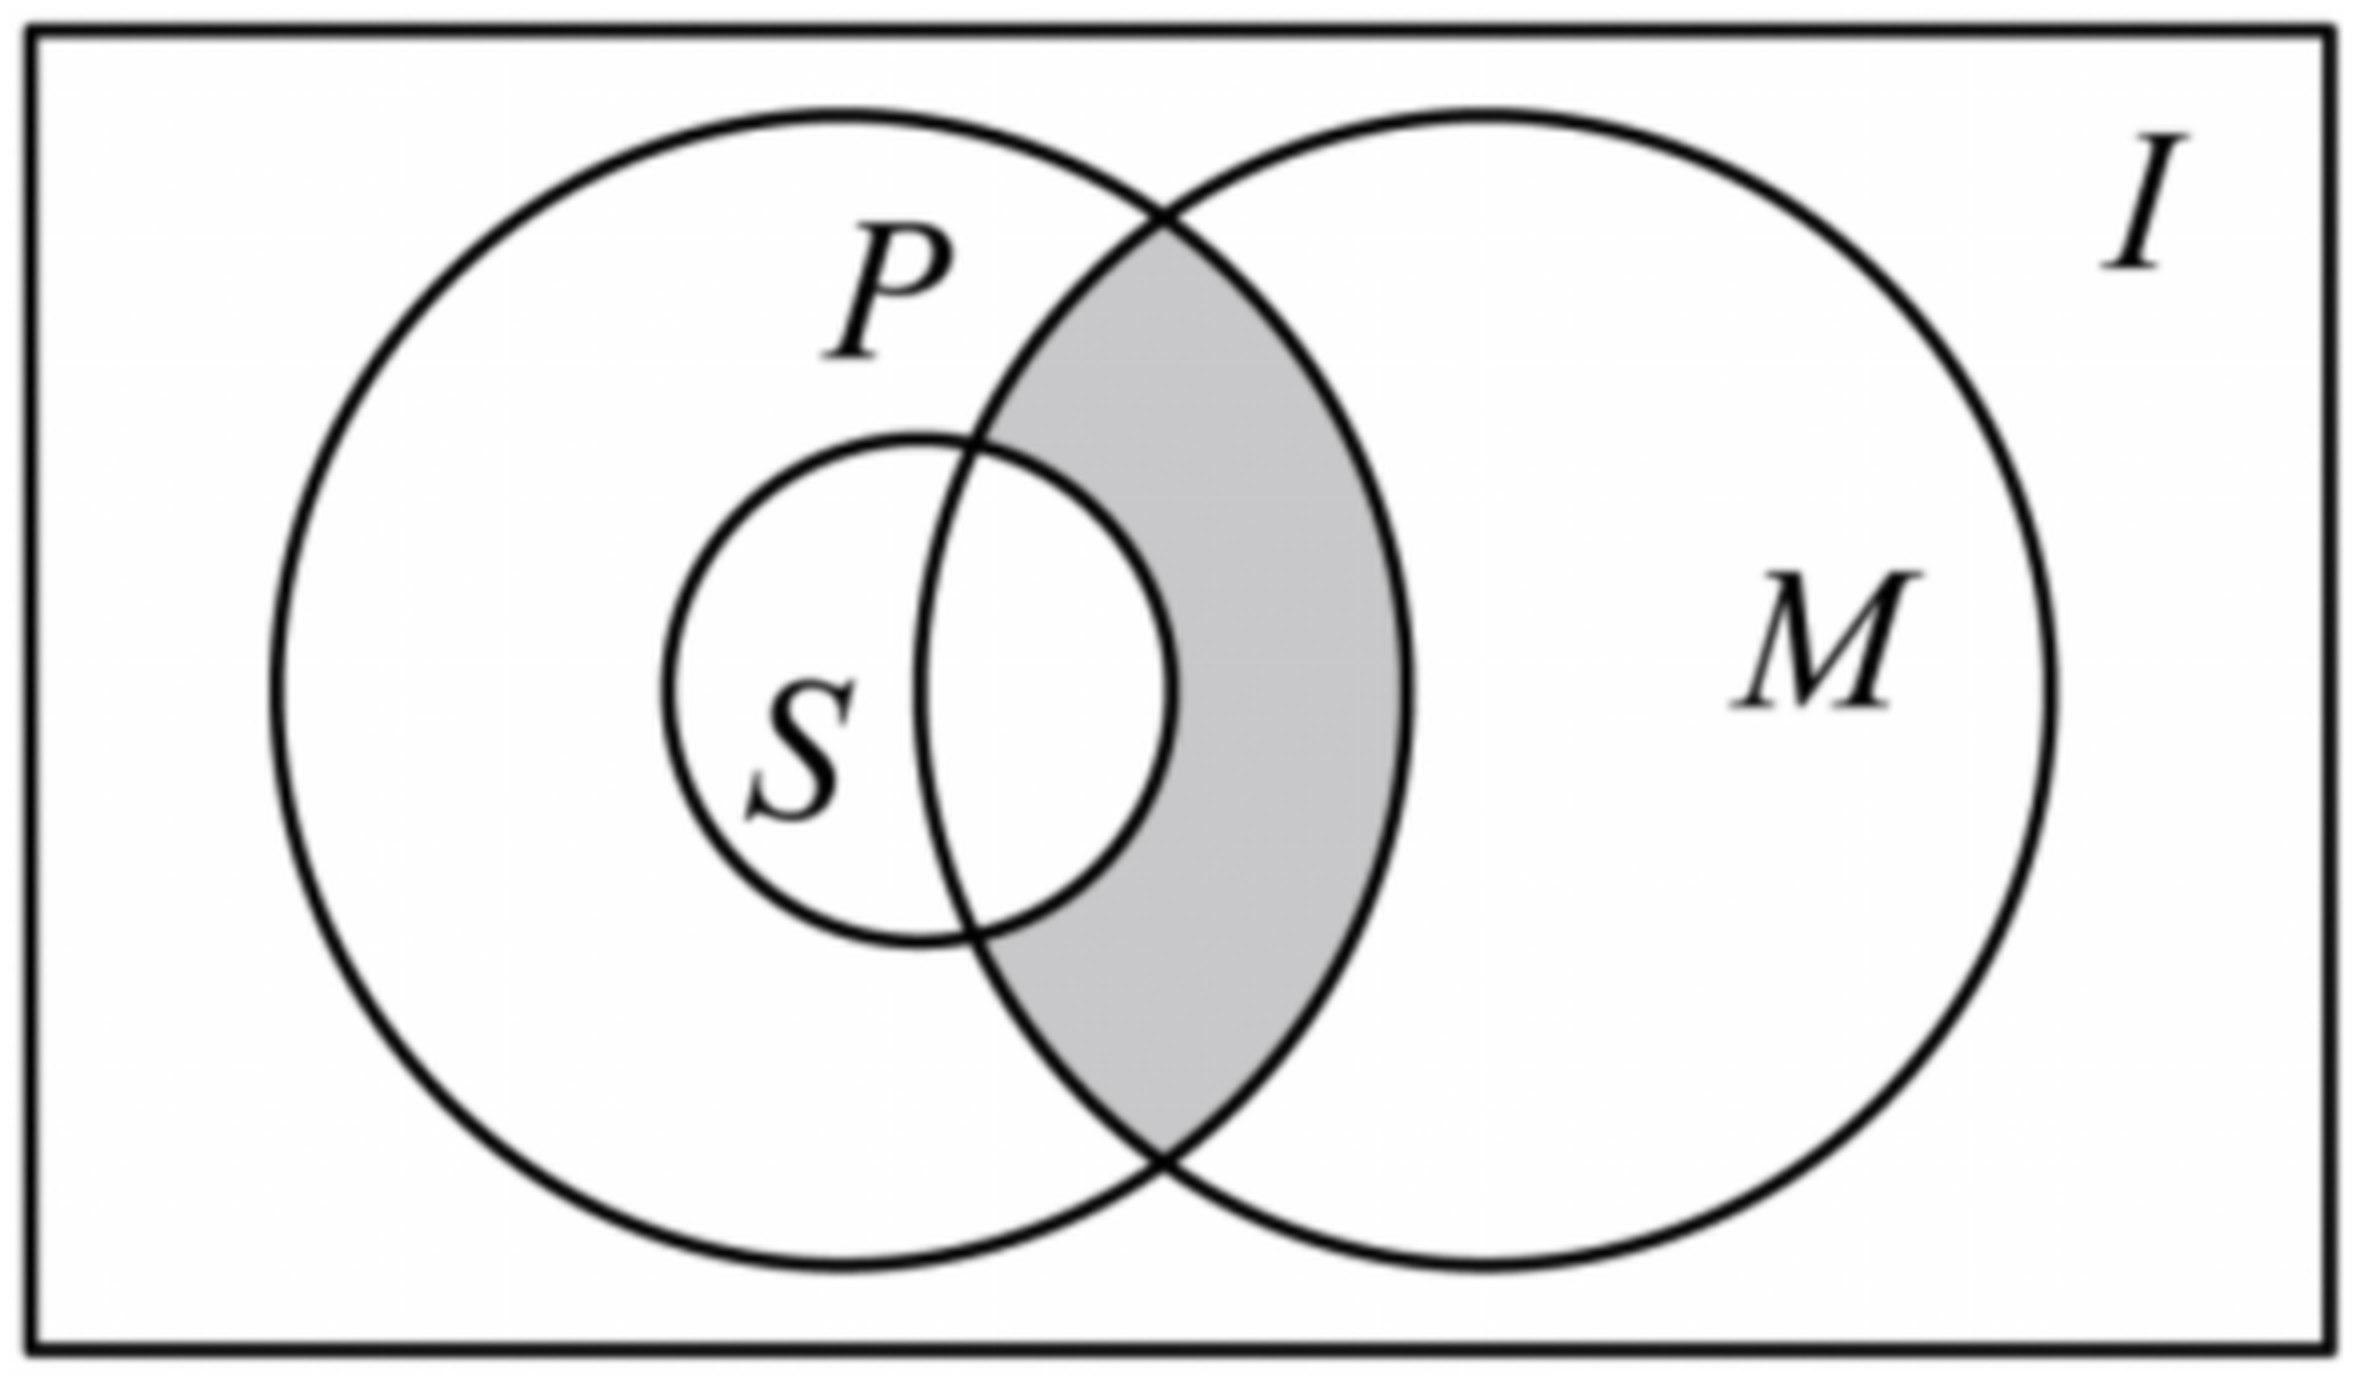
\includegraphics[width=0.46\textwidth]{figures/venn_MP_minus_S_h32.png}
\end{center}

\keepwithprev
A. $(M\cap P)\cap S$\qquad\qquad B. $(M\cap P)\cup S$

C. $(M\cap P)\cap\overline{S}$\qquad\qquad D. $(M\cap P)\cup\overline{S}$

\ans{$C$}

\ifanswer
\solbegin
\step{由 Venn 图得，集合表示 $M$、$P$ 的交集与 $S$ 的补集的交集，}
\step{即阴影部分所表示的集合是 $(M\cap P)\cap\overline{S}$. 故选 $C$.}
\solend

\fi

\item 若实数 $a$、$b$ 满足 $ab>0$，$a+2b=6$，则下列结论中错误的是\mbox{（\quad）}

\keepwithprev
A. $ab\leqslant\dfrac92$\qquad\qquad B. $a^2+4b^2\geqslant18$

C. $\dfrac1a+\dfrac2b$ 的最小值为 $\dfrac94$\qquad\qquad
D. $\dfrac{a^2}{a+1}+\dfrac{4b^2}{2b+1}$ 的最小值为 $\dfrac92$

\ans{$C$}

\ifanswer
\solbegin
\step{因为 $ab>0$，所以 $a$、$b$ 同号，又 $a+2b=6$，所以 $a$、$b$ 同正.}
\step{对于 $A$，由 $6=a+2b\geqslant2\sqrt{a\cdot2b}$ 得 $ab\leqslant\dfrac92$，故 $A$ 正确；}
\step{对于 $B$，由不等式 $\sqrt{\dfrac{m^2+n^2}2}\geqslant\dfrac{m+n}2$ 得
$\sqrt{\dfrac{a^2+(2b)^2}2}\geqslant\dfrac{a+2b}2=3$，}
\step{所以 $a^2+4b^2\geqslant18$，当且仅当 $a=2b=3$ 时取等号，故 $B$ 正确；}
\step{对于 $C$，$\dfrac1a+\dfrac2b
=\dfrac16\left(\dfrac1a+\dfrac2b\right)(a+2b)
=\dfrac16\left(5+\dfrac{2b}a+\dfrac{2a}b\right)$}
\step{$=\dfrac56+\dfrac13\left(\dfrac ba+\dfrac ab\right)
\geqslant\dfrac56+\dfrac13\times2\sqrt{\dfrac ba\cdot\dfrac ab}=\dfrac32$，}
\step{当且仅当 $\dfrac ba=\dfrac ab$，即 $a=b=2$ 时取等号，故 $C$ 错误；}
\step{对于 $D$，$\dfrac{a^2}{a+1}+\dfrac{4b^2}{2b+1}
=\dfrac{(a+1)^2-2(a+1)+1}{a+1}+\dfrac{(2b+1)^2-2(2b+1)+1}{2b+1}$}
\step{$=(a+1)-2+\dfrac1{a+1}+(2b+1)-2+\dfrac1{2b+1}
=(a+2b-2)+\dfrac1{a+1}+\dfrac1{2b+1}$}
\step{$=(6-2)+\dfrac{a+2b+2}{(a+1)(2b+1)}
=4+\dfrac8{(a+1)(2b+1)}$，}
\step{因为 $(a+1)(2b+1)\leqslant\left(\dfrac{a+1+2b+1}2\right)^2
=\left(\dfrac82\right)^2=16$，}
\step{当且仅当 $a+1=2b+1$，即 $a=2b=3$ 时取等号，}
\step{所以 $4+\dfrac8{(a+1)(2b+1)}\geqslant4+\dfrac8{16}=\dfrac92$，
故 $D$ 正确，其他几种方法同 12 题.}
\step{故选 $C$.}
\solend

\fi

% 注：本题的答案「D」原卷直接印在题干末尾的括号内，本稿按全稿惯例另提为 \ans{}。
\item 已知函数 $f(x)=x^2-2ax+a^2-1$，定义集合 $A=\{x\mid f(x)<0\}$. 若集合
$\{x\mid f(x)\in A\}=\varnothing$，则实数 $a$ 的取值范围是\mbox{（\quad）}

\keepwithprev
A. $(-3,-2)$\qquad B. $[-3,-2]$\qquad
C. $(-\infty,2)$\qquad D. $(-\infty,-2]$

\ans{$D$}

\item 非空集合 $A$ 具有如下性质：①若 $x$、$y\in A$，则 $\dfrac xy\in A$；
②若 $x$、$y\in A$，则 $x+y\in A$；

由此可知：下列判断中，错误的是\mbox{（\quad）}

\keepwithprev
A. $-1\notin A$\qquad\qquad B. $\dfrac{2025}{2026}\in A$

C. 若 $x$、$y\in A$，则 $xy\in A$\qquad\qquad
D. 若 $x$、$y\in A$，则 $x-y\in A$

\ans{$D$}

\ifanswer
\solbegin
\step{由题意得 $0\notin A$，$1\in A$，}
\step{对于 $A$，假设 $-1\in A$，则 $-1+1=0\in A$，矛盾，所以 $-1\notin A$，故 $A$ 正确；}
\step{对于 $B$，由 $1\in A$，得 $1+1=2\in A$，$2+1=3\in A$，…，$2025\in A$，$2026\in A$，}
\step{所以 $\dfrac{2025}{2026}\in A$，故 $B$ 正确；}
\step{对于 $C$，因为 $1\in A$，$x\in A$，所以 $\dfrac1x\in A$，
又因为 $y\in A$，所以 $\dfrac y{\frac1x}=xy\in A$，}
\step{故 $C$ 正确；}
\step{对于 $D$，因为 $1\in A$，$2\in A$，若 $x=1$，$y=2$，则 $x-y=-1\notin A$，故 $D$ 错误.}
\step{故选 $D$.}
\solend

\fi

\end{enumerate}

\bigsec{三、解答题}

\begin{enumerate}
\setcounter{enumi}{16}

\item 求下列关于实数 $x$ 的不等式的解集.

\begin{enumerate}[label=(\arabic*)]
\item $|2x+1|<5x-1$；
\item $\dfrac{(x-1)(x-3)(x-6)}{(x-2)(x-4)^2(x-5)}\geqslant0$.
\end{enumerate}

\ifanswer
\solbegin
\stepm{(1)}{因为不等式 $|2x+1|<5x-1$ 可化为 $-(5x-1)<2x+1<5x-1$，且 $5x-1>0$，}
\step{解得 $x>\dfrac23$，所以原不等式的解集为 $\left(\dfrac23,+\infty\right)$；}
\stepm{(2)}{不等式 $\dfrac{(x-1)(x-3)(x-6)}{(x-2)(x-4)^2(x-5)}\geqslant0$，}
\step{等价于 $(x-1)(x-3)(x-6)(x-2)(x-5)\geqslant0$，
且 $x-2\neq0$，$x-4\neq0$，$x-5\neq0$，}
\step{由“穿针引线法”，解得 $1\leqslant x<2$ 或 $3\leqslant x<4$ 或 $4<x<5$ 或 $x\geqslant6$，}
\step{所以不等式的解集为 $[1,2)\cup[3,4)\cup(4,5)\cup[6,+\infty)$.}
\solend

\fi

\ansspace[6]

\item 已知集合 $A=\left\{x\left|mx^2-mx+\dfrac{5m}2-6=0\right.\right\}\neq\varnothing$，
集合 $B=\{x\mid1<x<4$ 且 $x\in\Z\}$，$C=\{x\mid ax+3>0\}$；若 $A\cap B=A$.

\begin{enumerate}[label=(\arabic*)]
\item 求 $m$ 的取值范围.
\item 设 $m$ 的取值集合为 $D$，若 $C\cap D=\varnothing$，求 $m$ 的值及其对应 $a$ 的取值范围.
\end{enumerate}

\ans{略}

\ansspace[8]

\item 已知函数 $f(x)=x^2+(m-2)x+2m-1$.

\begin{enumerate}[label=(\arabic*)]
\item 若 $f(x)=0$ 的两根为 $x_1$、$x_2$，且 $|x_1-x_2|=2$，求实数 $m$ 的值；
\item 若函数 $y=f(x)$ 的图像在区间 $(0,1)$ 上与 $x$ 轴只有一个交点，
求实数 $m$ 的取值范围.
\end{enumerate}

\ifanswer
\solbegin
\stepm{(1)}{由题意得 $x_1+x_2=-(m-2)=2-m$，$x_1x_2=2m-1$，}
\step{由 $|x_1-x_2|=\sqrt{(x_1+x_2)^2-4x_1x_2}
=\sqrt{(2-m)^2-4(2m-1)}=2$，}
\step{化简得 $m^2-12m+4=0$，解得 $m=6\pm4\sqrt2$，故 $m=6\pm4\sqrt2$.}
\stepm{(2)}{当 $f(x)=0$ 只有一个根，且此根位于区间 $(0,1)$，}
\step{则 $\begin{cases}0<\dfrac{2-m}2<1\\[4pt]
\Delta=(m-2)^2-4(2m-1)=0\end{cases}$，
解得 $\begin{cases}0<m<2\\ m=6-2\sqrt7\text{ 或 }m=6+2\sqrt7\end{cases}$，}
\step{所以 $m=6-2\sqrt7$；}
\step{当 $f(x)=0$ 有两个根时，有一个根在区间 $(0,1)$ 内，且另一个根位于 $[0,1]$ 之外，}
\step{则 $\begin{cases}f(0)f(1)<0\\ \Delta=(m-2)^2-4(2m-1)>0\end{cases}$，
解得 $\begin{cases}\dfrac12<m<\dfrac23\\[4pt]
m<6-2\sqrt7\text{ 或 }m>6+2\sqrt7\end{cases}$，}
% 注：下一行原卷作「即 $\dfrac12<m<\dfrac32$」，按上一行方程组应为
%     $\dfrac12<m<\dfrac23$（同页最终答案也印证），照录未改，见文件头「原卷存疑」①。
\step{即 $\dfrac12<m<\dfrac32$；}
\step{当 $f(x)=0$ 有两个根位于区间 $[0,1]$ 内，且只有一个根在区间 $(0,1)$ 内，}
\step{则另一个根为 $0$ 时，得 $m=\dfrac12$，此时 $x_1+x_2=\dfrac32$，
解得另一个根 $x_2=\dfrac32>0$，故此种情况不符题意；}
\step{当 $f(x)=0$ 有两个根位于区间 $(0,1]$ 内，且只有一个根在区间 $(0,1)$ 内，}
\step{则另一个根为 $1$ 时，得 $m=\dfrac23$，此时 $x_1+x_2=\dfrac43$，
解得另一个根 $x_2=\dfrac13$，故此种情况符合题意；}
\step{综上所述，$m$ 的取值范围为
$\left(\dfrac12,\dfrac23\right]\cup\{6-2\sqrt7\}$.}
\solend

\fi

\ansspace[8]

\item 设集合 $A=\{a_1,a_2,a_3,a_4\}$，$B=\{b_1,b_2,b_3,b_4\}$，$C=\{2,3,4,6\}$，
新定义：集合 $A$ 中所有含 $k$ 个元素的子集中 $k$ 个元素之和组成的集合为“$k$ 元集和集”，
集合 $A$ 中所有含 $k$ 个元素的子集中最大元素减去剩余所有元素的和组成的集合为“$k$ 元差集”.

\begin{enumerate}[label=(\arabic*)]
\item 若 $A$ 的“$k$ 元集和集”为 $C$，求：集合 $A$.
\item 在 (1) 的条件下，若 $B$ 的“$k$ 元差集”为 $C$，求：所有满足条件的 $A\cap B$ 的真子集
个数之和.
\item 设 $b_1=a_1^2$，$b_2=a_2^2$，$b_3=a_3^2$，$b_4=a_4^2$，若 $A\cap B$ 为 $2$ 元集且
元素之和为 $10$ 且 $A$ 的“$2$ 元集和集”中最大元素不超过 $14$，求：所有满足条件的 $A$ 的
“$3$ 元差集”.
\end{enumerate}

\ifanswer
\solbegin
\stepm{(1)}{若 $A$ 的“$k$ 元集和集”为 $C$，$C=\{2,3,4,6\}$，则集合为 $\{-1,1,2,3\}$；}
\stepm{(2)}{$B$ 集合为 $\{5,3,0,-1\}$ 或 $\{9,3,1,0\}$ 或 $\{6,3,1,-1\}$，}
\step{故所有 $A\cap B$ 的真子集个数之和为 $13$；}
\stepm{(3)}{$b_1=a_1^2$，$b_2=a_2^2$，$b_3=a_3^2$，$b_4=a_4^2$，}
\step{若 $A\cap B$ 为 $2$ 元集且元素之和为 $10$，
且 $A$ 的“$2$ 元集和集”中最大元素不超过 $14$，}
% 注：下一行答案的第二个集合 $\{0,4,5,6\}$ 是 4 元集，而题问的却是「3 元差集」，
%     原卷如此，照录未改，见文件头「原卷存疑」③。
\step{则满足条件的 $A$ 的“$3$ 元差集” $\{1,3,5\}$ 或 $\{0,4,5,6\}$ 或 $\{2,4,5,8\}$.}
\solend

\fi

\ansspace[8]

\item 已知有限集 $X$、$Y$，定义集合 $X-Y=\{x\mid x\in X$ 且 $x\notin Y\}$，
$|X|$ 表示集合 $X$ 元素个数.

\begin{enumerate}[label=(\arabic*)]
\item 若 $X=\{1,2,3,4\}$，$Y=\{3,4,5\}$，写出集合 $X-Y$ 和 $Y-X$，以及
$|(X-Y)\cup(Y-X)|$ 的值；
\item 给定正整数 $n$，集合 $S=\{1,2,\cdots,n\}$，对于实数集的非空有限子集 $A$、$B$，
定义集合 $C=\{x\mid x=a+b,a\in A,b\in B\}$；

①求证：$|A-S|+|B-S|+|S-C|\geqslant1$；

②求 $|(A-S)\cup(S-A)|+|(B-S)\cup(S-B)|+|(C-S)\cup(S-C)|$ 的最小值.
\end{enumerate}

\ifanswer
\solbegin
\stepm{(1)}{由定义直接得 $X-Y=\{1,2\}$，$Y-X=\{5\}$，
$|(X-Y)\cup(Y-X)|=3$.}
% 注：下一句原卷作「显然 $|X|\geqslant0$」（按后文论证疑为 $|S|\geqslant0$），
%     照录未改，见文件头「原卷存疑」②。
\stepm{(2)}{①显然 $|X|\geqslant0$.}
\step{若 $A\cup B$ 中含有一个不在 $S$ 中的元素，则 $|A-S|+|B-S|\geqslant1$，
即 $|A-S|+|B-S|+|S-C|\geqslant1$.}
\step{若 $A\sub S$，且 $B\sub S$，则 $|A-S|=|B-S|=0$；}
\step{此时 $A$ 中最小的元素 $a\geqslant1$，$B$ 中最小的元素 $b\geqslant1$，
所以 $C$ 中最小的元素 $a+b\geqslant2$，所以 $1\notin C$.}
\step{因为 $S=\{1,2,\cdots,n\}$，所以 $|S-C|\geqslant1$，
即 $|A-S|+|B-S|+|S-C|\geqslant1$.}
\step{综上，$|A-S|+|B-S|+|S-C|\geqslant1$.}
\step{②由①得 $|A-S|+|B-S|+|S-C|\geqslant1$.}
\step{所以 $|(A-S)\cup(S-A)|+|(B-S)\cup(S-B)|+|(C-S)\cup(S-C)|$}
\step{$=|A-S|+|S-A|+|B-S|+|S-B|+|C-S|+|S-C|$}
\step{$\geqslant|S-A|+|S-B|+|C-S|+1$.}
\step{若 $A\cap S=\varnothing$，或 $B\cap S=\varnothing$，则 $|S-A|+|S-B|\geqslant n$.}
\step{若 $A\cap S\neq\varnothing$，且 $B\cap S\neq\varnothing$，
设 $A\cap S=\{a_1,a_2,\cdots,a_s\}$，$B\cap S=\{b_1,b_2,\cdots,b_t\}$，}
\step{且 $1\leqslant a_1<a_2<\cdots<a_s\leqslant n$，
$1\leqslant b_1<b_2<\cdots<b_t\leqslant n$，则 $|S-A|=n-s$，$|B-S|=n-t$.}
% 注：原卷的解析到此为止（第 10 页末），②的最小值并未给出，照录未补，
%     见文件头「原卷存疑」④。
\solend

\fi

\ansspace*[10]

\end{enumerate}

\end{document}
"
%
% 原始材料是微信公众号图文（公众号「魔都数学加油站」连载「27学年高一 32」，2026-09-25 发布，
% 原文标题「27学年高一32——2026-2027年上海市华师大二附中高一上周末作业4」），
% 正文为 10 张 PNG 页。**同一篇里各页分辨率不一致**（2560×3620 与 4762×6735 两档混排），
% 取 mmbiz.qpic.cn/<hash>/0 的原图档。原文本身就是一份**讲评版**——有的题下方印【解析】、
% 有的印【答案】，第 15 题的答案直接印在题干末尾的括号里。
% 试题文字、答案与解析均照原卷录入，未改内容。卷面的粉色斜水印属水印，未录入。
%
% ⚠ 卷首年份：本卷卷面印作「**2025-2026 年**」，与连载「27学年高一32」及公众号原文标题的
%   「2026-2027 年」**不一致**。经三人次分别把标题行裁出放大（4×—10×）独立判读，三次都读作
%   2025-2026，且校名作「华师大二附中」（无「东」字）、卷面亦无「上海市」三字。
%   按全稿「标题行照原卷」的口径，本稿照卷面排作「2025--2026 年…」——这是全稿唯一一份
%   年份不是 2026--2027 的卷子（其余 35 份均为 2026--2027）。
%
% 卷首标题：原卷印作「……年华师大二附中高一上周末作业 4」（公众号标题里的「上海市」
% 三字卷面标题行没有，本稿照卷面），年份区间按全稿惯例排 en dash，前缀照原卷保留「年」。
%
% 与原卷的排版差异（均已在 README「说明」中交代）：
%   ① 原文自**第 3 题**起（第 1、2 题未在该文中发布），故本稿题号亦自 3 起；
%   ② 原卷本就印有「一、填空题」「二、选择题」「三、解答题」三节标题，本稿照原卷分节，
%      只把标题改排成全稿统一的「大节标题」样式；
%   ③ 原卷第 6、8、9 题只印【答案】行（第 18 题的【答案】印作「略”），其余各题印【解析】，
%      第 15 题的答案直接印在题干末尾的括号内；本稿统一改为试卷版隐去、
%      答案版以 \ans{}／\ifanswer 块给出，两版彻底分离；
%   ④ 子集符号原卷两种并用：第 21(2)① 的 $A\sub S$、$B\sub S$ 带下划线，
%      第 3、10 题的 $(0,2)\subset(-\infty,3)$、$A\subset B$、$\overline{B}\subset\overline{A}$
%      作真包含，本稿分别照录为 $\sub$ 与 $\subset$；
%   ⑤ 补集符号原卷一律作上横线（$\overline{A}$、$\overline{B}$、$\overline{S}$），本稿照录；
%      空集原卷作「斜杠伸出圆外」的 $\varnothing$；
%   ⑥ 判别式记号原卷两种：第 4 题作粗体的 $\Delta$、第 11 题作细等宽的 $\triangle$，本稿照录；
%   ⑦ 数集记号原卷作斜体的 $R$、$Z$（第 4、18 题），本稿按全稿惯例统一写作 $\R$、$\Z$；
%   ⑧ 原卷填空的横线约两个字宽，本稿按全稿惯例统一排 \blankline[4.4em]；
%   ⑨ 原卷未印副标题，本稿按全稿惯例补出副标题「集合与常用逻辑用语」；
%   ⑩ 本卷只有第 13 题一图（韦恩图），原卷印在题干右侧，本稿移至题干之后；
%      图取原卷截图、4× LANCZOS 放大（figures/venn_MP_minus_S_h32.png）。
%
% 原卷存疑四处（均照抄原卷、未改，见源码中该处上方注释）：
%   ① 第 19(2)【解析】有「即 $\dfrac12<m<\dfrac32$」，按上一行的方程组应为
%      $\dfrac12<m<\dfrac23$（同页最终答案 $\left(\dfrac12,\dfrac23\right]$ 也印证）；
%   ② 第 21(2)① 首句作「显然 $|X|\geqslant0$」（按后文论证疑为 $|S|\geqslant0$）；
%   ③ 第 20(3) 的答案第二个集合 $\{0,4,5,6\}$ 是 4 元集，而题问的是「3 元差集」；
%   ④ 第 21(2)② 的解析**原卷就未写完**（第 10 页到「则 $|S-A|=n-s$，$|B-S|=n-t$」即止）。

\documentclass[a4paper,11pt]{article}
\usepackage{common}

\begin{document}

\examtitlest[3]{2025--2026 年华师大二附中高一上周末作业 4}{集合与常用逻辑用语}

\bigsec{一、填空题}

\begin{enumerate}
\setcounter{enumi}{2}

\item 设 $x$ 为实数，则“$x<3$”是“$x(x-2)<0$”的 \blankline[4.4em] 条件.

\ifanswer
\solbegin
\step{$x(x-2)<0$，解得 $0<x<2$，$(0,2)\subset(-\infty,3)$，}
\step{若 $x$ 属于“$x(x-2)<0$”，则属于“$x<3$”一定成立，即满足必要性，}
\step{若 $x$ 属于“$x<3$”，不一定满足“$x(x-2)<0$”，如 $x=-1$，即充分性不成立；}
\step{故“$x<3$”是“$x(x-2)<0$”的必要不充分条件.}
\solend

\fi

\item 若关于 $x$ 的不等式 $kx^2-kx+1>0$ 的解集为 $\R$，则实数 $k$ 的取值范围为
\blankline[4.4em].

\ifanswer
\solbegin
\step{①当 $k=0$ 时，不等式为 $1>0$ 恒成立，满足题意；}
\step{②当 $k\neq0$ 时，只要 $\begin{cases}k>0\\ \Delta=k^2-4k<0\end{cases}$，
解得 $0<k<4$；}
\step{所以不等式 $kx^2-kx+1>0$ 的解集为 $\R$，则实数 $k$ 的取值范围为 $[0,4)$.}
\solend

\fi

\item 已知 $1<a<3$，$-5<b<-2$，则 $\dfrac ab$ 的取值范围是 \blankline[4.4em].

\ifanswer
\solbegin
\step{因为 $-5<b<-2$，所以 $2<-b<5$，$\dfrac15<-\dfrac1b<\dfrac12$，又 $1<a<3$，}
\step{得 $\dfrac15<-\dfrac ab<\dfrac32$，则 $-\dfrac32<\dfrac ab<-\dfrac15$，
故 $\dfrac ab$ 的取值范围是 $\left(-\dfrac32,-\dfrac15\right)$.}
\solend

\fi

\item 关于 $x$ 的不等式 $\dfrac{ax-1}{x-a}>1$ 的解集为 $A$，且 $3\notin A$，
则实数 $a$ 的取值范围为 \blankline[4.4em].

\ans{$(-\infty,1]\cup[3,+\infty)$}

\item 若关于 $x$ 的不等式 $a\leqslant\dfrac34x^2-3x+4\leqslant b$ 的解集恰好是 $[a,b]$，
则 $b-a=$ \blankline[4.4em].

\ifanswer
\solbegin
\step{令 $f(x)=\dfrac34x^2-3x+4$，则 $f(x)$ 的对称轴为 $x=2$，}
\step{画出函数 $f(x)=\dfrac34x^2-3x+4=\dfrac34(x-2)^2+1$ 的图象，
得 $f(x)_{\min}=f(2)=1$，}
\step{由题意得 $a\leqslant1$，且 $f(a)=f(b)=b$，$a<b$，}
\step{由 $f(b)=b$ 得 $\dfrac34b^2-3b+4=b$，解得 $b=\dfrac43$（舍去）或 $b=4$，得 $b=4$，}
\step{由抛物线的对称轴为 $x=2$ 得 $a=0$，所以 $b-a=4$.}
\solend

\fi

\item 若关于 $x$ 的方程 $x^2-2kx+k+4=0$ 在 $[1,2]$ 上有解，则实数 $k$ 的取值范围为
\blankline[4.4em].

\ans{$\left[\dfrac83,5\right]$}

\item 记关于 $x$ 的方程 $x^2-2mx-2m+3=0$ 的两实根为 $x_1$、$x_2$，
则 $(x_1-2)^2+(x_2-2)^2$ 的最小值为 \blankline[4.4em].

\ans{$2$}

\item 若“$|mx^2-4x+3|\geqslant2$”的必要非充分条件是“$x\leqslant1$ 或 $x\geqslant4$”，
则实数 $m$ 的取值范围是 \blankline[4.4em].

\ifanswer
\solbegin
\step{记 $|mx^2-4x+3|\geqslant2$ 的解集为集合 $A$，
$B=\{x\mid x\leqslant1\text{ 或 }x\geqslant4\}$，}
\step{则 $\overline{A}$ 为 $|mx^2-4x+3|<2$ 的解集，$\overline{B}=\{x\mid1<x<4\}$；}
\step{因为 $B$ 是 $A$ 的必要非充分条件，所以 $A\subset B$，
得 $\overline{B}\subset\overline{A}$，}
\step{即对任意 $x\in(1,4)$，都有 $|mx^2-4x+3|<2$ 恒成立.}
\step{因为 $|mx^2-4x+3|<2$，$1<x<4$，所以 $-2<mx^2-4x+3<2$，}
\step{化简得
$-5\left(\dfrac1x\right)^2+4\left(\dfrac1x\right)
<m<-\left(\dfrac1x\right)^2+4\left(\dfrac1x\right)$；}
\step{令 $t=\dfrac1x$，$g(t)=-5t^2+4t$，$h(t)=-t^2+4t$，
且 $t\in\left(\dfrac14,1\right)$；}
\step{所以 $g(t)=-5t^2+4t=-5\left(t-\dfrac25\right)^2+\dfrac45$，
当 $t=\dfrac25$ 时，$g(t)$ 取得最大值 $\dfrac45$，}
\step{$h(t)=-t^2+4t=-(t-2)^2+4$，当 $t=\dfrac14$ 时，$h(t)$ 取得最小值，
即 $h(t)>h\left(\dfrac14\right)=\dfrac{15}{16}$；}
\step{因为对任意 $t\in\left(\dfrac14,1\right)$，$g(t)<m<h(t)$ 恒成立，
所以 $g\left(\dfrac25\right)<m\leqslant h\left(\dfrac14\right)$，}
\step{即 $\dfrac45<m\leqslant\dfrac{15}{16}$，
所以 $m$ 的取值范围是 $\left(\dfrac45,\dfrac{15}{16}\right]$.}
\solend

\fi

\item 已知关于 $x$ 的方程 $x^2+2(m-2)x+m^2-3m+3=0$ 有两个不相等的实数根 $x_1$、$x_2$，则

$\dfrac{mx_1}{x_1-1}+\dfrac{mx_2}{x_2-1}-\dfrac2{x_1+x_2-2}$ 的最大值为 \blankline[4.4em].

\ifanswer
\solbegin
\step{关于 $x$ 的方程 $x^2+2(m-2)x+m^2-3m+3=0$ 有两个不相等的实数根 $x_1$、$x_2$，}
\step{则 $\triangle=4(m-2)^2-4(m^2-3m+3)=-4m+4>0$，得 $m<1$，}
\step{且 $x_1+x_2=-2(m-2)$，$x_1x_2=m^2-3m+3$，}
\step{$\dfrac{mx_1}{x_1-1}+\dfrac{mx_2}{x_2-1}-\dfrac2{x_1+x_2-2}
=\dfrac{m[2x_1x_2-(x_1+x_2)]}{x_1x_2-(x_1+x_2)+1}+\dfrac1{m-1}$}
\step{$=\dfrac{2m(m-1)^2}{m^2-m}+\dfrac1{m-1}=2(m-1)+\dfrac1{m-1}$，}
\step{又因为 $m<1$，所以 $m-1<0$，则 $1-m>0$，}
\step{所以 $2(1-m)+\dfrac1{1-m}\geqslant2\sqrt{2(1-m)\cdot\dfrac1{1-m}}=2\sqrt2$，}
\step{当且仅当 $2(1-m)=\dfrac1{1-m}$ 时，即 $m=1-\dfrac{\sqrt2}2$ 时取等号，}
\step{所以 $2(m-1)+\dfrac1{m-1}\leqslant-2\sqrt2$，
即 $\dfrac{mx_1}{x_1-1}+\dfrac{mx_2}{x_2-1}-\dfrac2{x_1+x_2-2}$ 的最大值为 $-2\sqrt2$.}
\solend

\fi

\item 若正实数 $a$、$b$ 满足 $a+2b=ab$，则 $\dfrac4{a^2+2a}+\dfrac1{2b^2+b}$ 的最小值是
\blankline[4.4em].

\ifanswer
\solbegin
\stepm{法一}{由 $a+2b=ab$，得 $\dfrac2a+\dfrac1b=1$，}
\step{令 $x=\dfrac1a$，$y=\dfrac1b$，则 $x$、$y>0$，$2x+y=1$，$2x+1+y+2=4$，}
\step{所以 $\dfrac4{a^2+2a}+\dfrac1{2b^2+b}
=\dfrac4{\frac1{x^2}+\frac2x}+\dfrac1{\frac2{y^2}+\frac1y}
=\dfrac{4x^2}{2x+1}+\dfrac{y^2}{y+2}$（*）}
\step{$=\dfrac{(2x+1)^2-2(2x+1)+1}{2x+1}+\dfrac{(y+2)^2-4(y+2)+4}{y+2}$}
\step{$=2x-1+\dfrac1{2x+1}+y-2+\dfrac4{y+2}=\dfrac1{2x+1}+\dfrac4{y+2}-2$}
\step{$=\dfrac14\left(\dfrac1{2x+1}+\dfrac4{y+2}\right)(2x+1+y+2)-2$}
\step{$=\dfrac14\left[5+\dfrac{y+2}{2x+1}+\dfrac{4(2x+1)}{y+2}\right]-2
\geqslant\dfrac14(5+2\sqrt4)-2=\dfrac14$，}
\step{当且仅当 $\dfrac{y+2}{2x+1}=\dfrac{4(2x+1)}{y+2}$，
即 $x=\dfrac16$，$y=\dfrac23$ 时取等号，}
\step{故 $\dfrac4{a^2+2a}+\dfrac1{2b^2+b}$ 的最小值是 $\dfrac14$.}
\stepm{法二}{在法一（*）后，由权方和不等式，得
$\dfrac4{a^2+2a}+\dfrac1{2b^2+b}
=\dfrac{4x^2}{2x+1}+\dfrac{y^2}{y+2}
\geqslant\dfrac{(2x+y)^2}{2x+1+y+2}=\dfrac14$，}
\step{当且仅当……，故 $\dfrac4{a^2+2a}+\dfrac1{2b^2+b}$ 的最小值是 $\dfrac14$.}
\stepm{法三}{注意到
$\left(\dfrac{a+2}a+\dfrac{2b+1}b\right)\left(\dfrac4{a^2+2a}+\dfrac1{2b^2+b}\right)$}
\step{$\geqslant
\left(\sqrt{\dfrac{a+2}a\cdot\dfrac4{a^2+2a}}
+\sqrt{\dfrac{2b+1}b\cdot\dfrac1{2b^2+b}}\right)^2
=\left(\dfrac2a+\dfrac1b\right)^2$，}
\step{其中 $\dfrac{a+2}a+\dfrac{2b+1}b=3+\dfrac{a+2b}{ab}=4$，
$\dfrac2a+\dfrac1b=\dfrac{a+2b}{ab}=1$，}
\step{所以 $\dfrac4{a^2+2a}+\dfrac1{2b^2+b}\geqslant\dfrac14$，
当且仅当……，故 $\dfrac4{a^2+2a}+\dfrac1{2b^2+b}$ 的最小值是 $\dfrac14$.}
\solend

\fi

\end{enumerate}

\bigsec{二、选择题}

\begin{enumerate}
\setcounter{enumi}{12}

\item 如图，$I$ 为全集，$M$、$P$、$S$ 是 $I$ 的三个子集，则阴影部分所表示的集合是
\mbox{（\quad）}

\begin{center}
% 图取原卷截图、4× LANCZOS 放大（原卷把图印在题干右侧，本稿移至此处，见文件头⑩）。
% 矩形为全集 $I$，左大圆 $P$（内下方含小圆 $S$，其右侧伸入 $P$ 与 $M$ 的重叠区）、
% 右大圆 $M$；阴影是 $P$、$M$ 重叠的透镜形区域挖掉 $S$ 后剩下的部分（左缘呈弯月形）。
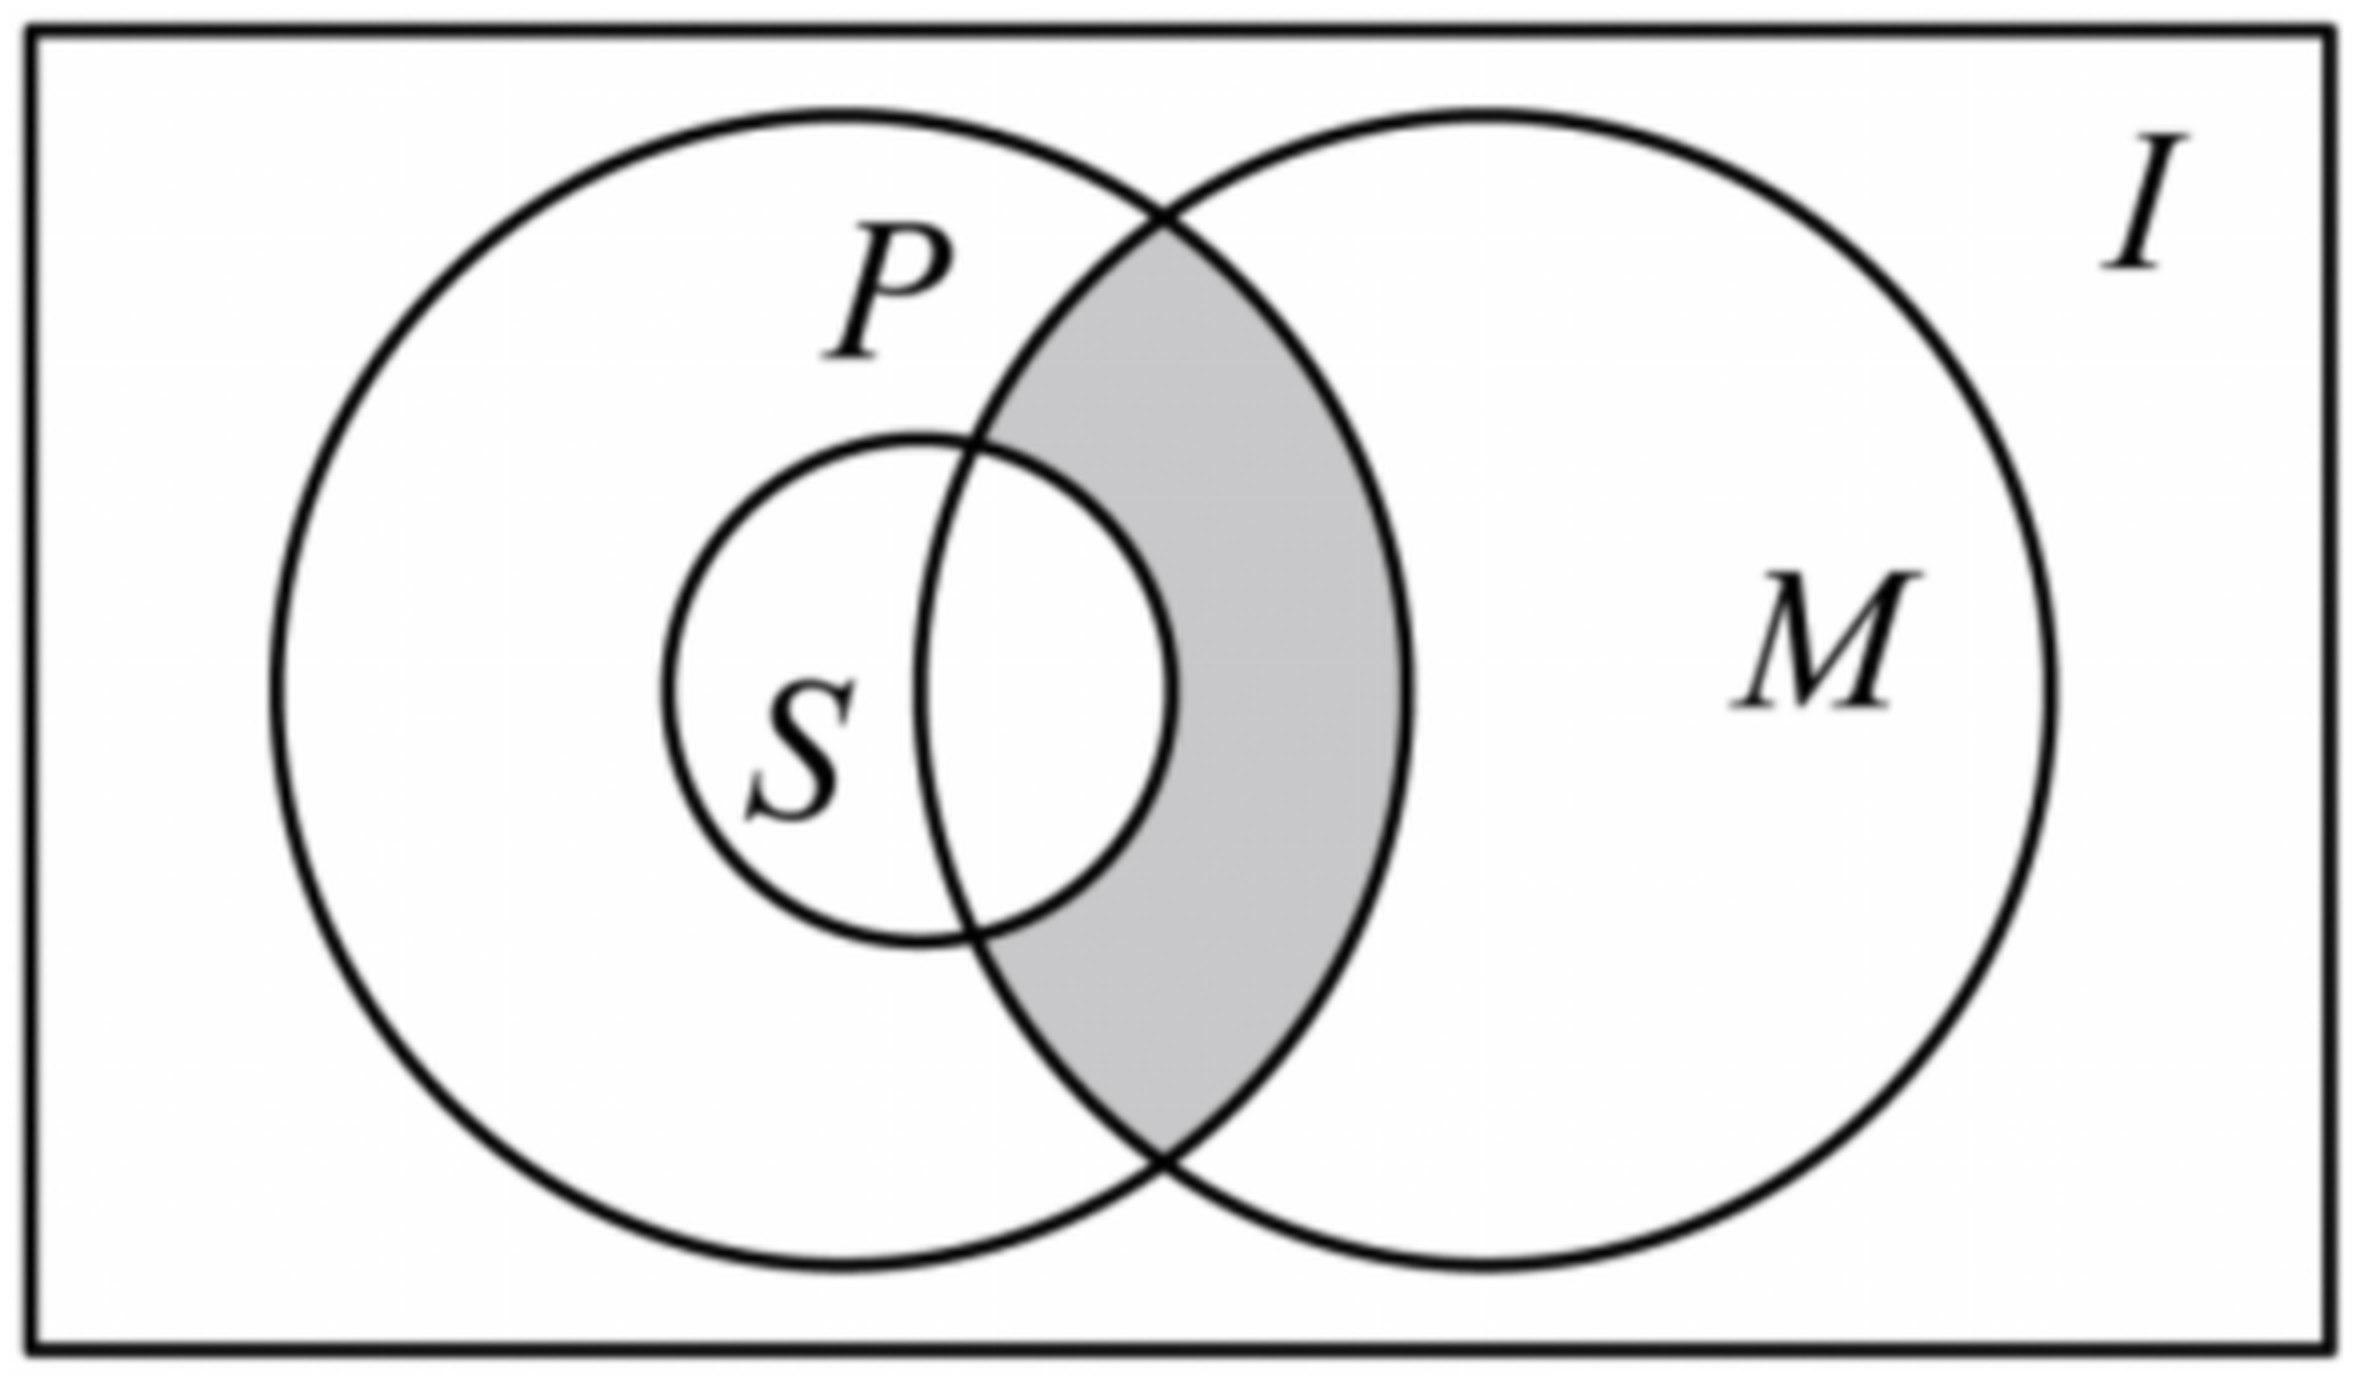
\includegraphics[width=0.46\textwidth]{figures/venn_MP_minus_S_h32.png}
\end{center}

\keepwithprev
A. $(M\cap P)\cap S$\qquad\qquad B. $(M\cap P)\cup S$

C. $(M\cap P)\cap\overline{S}$\qquad\qquad D. $(M\cap P)\cup\overline{S}$

\ans{$C$}

\ifanswer
\solbegin
\step{由 Venn 图得，集合表示 $M$、$P$ 的交集与 $S$ 的补集的交集，}
\step{即阴影部分所表示的集合是 $(M\cap P)\cap\overline{S}$. 故选 $C$.}
\solend

\fi

\item 若实数 $a$、$b$ 满足 $ab>0$，$a+2b=6$，则下列结论中错误的是\mbox{（\quad）}

\keepwithprev
A. $ab\leqslant\dfrac92$\qquad\qquad B. $a^2+4b^2\geqslant18$

C. $\dfrac1a+\dfrac2b$ 的最小值为 $\dfrac94$\qquad\qquad
D. $\dfrac{a^2}{a+1}+\dfrac{4b^2}{2b+1}$ 的最小值为 $\dfrac92$

\ans{$C$}

\ifanswer
\solbegin
\step{因为 $ab>0$，所以 $a$、$b$ 同号，又 $a+2b=6$，所以 $a$、$b$ 同正.}
\step{对于 $A$，由 $6=a+2b\geqslant2\sqrt{a\cdot2b}$ 得 $ab\leqslant\dfrac92$，故 $A$ 正确；}
\step{对于 $B$，由不等式 $\sqrt{\dfrac{m^2+n^2}2}\geqslant\dfrac{m+n}2$ 得
$\sqrt{\dfrac{a^2+(2b)^2}2}\geqslant\dfrac{a+2b}2=3$，}
\step{所以 $a^2+4b^2\geqslant18$，当且仅当 $a=2b=3$ 时取等号，故 $B$ 正确；}
\step{对于 $C$，$\dfrac1a+\dfrac2b
=\dfrac16\left(\dfrac1a+\dfrac2b\right)(a+2b)
=\dfrac16\left(5+\dfrac{2b}a+\dfrac{2a}b\right)$}
\step{$=\dfrac56+\dfrac13\left(\dfrac ba+\dfrac ab\right)
\geqslant\dfrac56+\dfrac13\times2\sqrt{\dfrac ba\cdot\dfrac ab}=\dfrac32$，}
\step{当且仅当 $\dfrac ba=\dfrac ab$，即 $a=b=2$ 时取等号，故 $C$ 错误；}
\step{对于 $D$，$\dfrac{a^2}{a+1}+\dfrac{4b^2}{2b+1}
=\dfrac{(a+1)^2-2(a+1)+1}{a+1}+\dfrac{(2b+1)^2-2(2b+1)+1}{2b+1}$}
\step{$=(a+1)-2+\dfrac1{a+1}+(2b+1)-2+\dfrac1{2b+1}
=(a+2b-2)+\dfrac1{a+1}+\dfrac1{2b+1}$}
\step{$=(6-2)+\dfrac{a+2b+2}{(a+1)(2b+1)}
=4+\dfrac8{(a+1)(2b+1)}$，}
\step{因为 $(a+1)(2b+1)\leqslant\left(\dfrac{a+1+2b+1}2\right)^2
=\left(\dfrac82\right)^2=16$，}
\step{当且仅当 $a+1=2b+1$，即 $a=2b=3$ 时取等号，}
\step{所以 $4+\dfrac8{(a+1)(2b+1)}\geqslant4+\dfrac8{16}=\dfrac92$，
故 $D$ 正确，其他几种方法同 12 题.}
\step{故选 $C$.}
\solend

\fi

% 注：本题的答案「D」原卷直接印在题干末尾的括号内，本稿按全稿惯例另提为 \ans{}。
\item 已知函数 $f(x)=x^2-2ax+a^2-1$，定义集合 $A=\{x\mid f(x)<0\}$. 若集合
$\{x\mid f(x)\in A\}=\varnothing$，则实数 $a$ 的取值范围是\mbox{（\quad）}

\keepwithprev
A. $(-3,-2)$\qquad B. $[-3,-2]$\qquad
C. $(-\infty,2)$\qquad D. $(-\infty,-2]$

\ans{$D$}

\item 非空集合 $A$ 具有如下性质：①若 $x$、$y\in A$，则 $\dfrac xy\in A$；
②若 $x$、$y\in A$，则 $x+y\in A$；

由此可知：下列判断中，错误的是\mbox{（\quad）}

\keepwithprev
A. $-1\notin A$\qquad\qquad B. $\dfrac{2025}{2026}\in A$

C. 若 $x$、$y\in A$，则 $xy\in A$\qquad\qquad
D. 若 $x$、$y\in A$，则 $x-y\in A$

\ans{$D$}

\ifanswer
\solbegin
\step{由题意得 $0\notin A$，$1\in A$，}
\step{对于 $A$，假设 $-1\in A$，则 $-1+1=0\in A$，矛盾，所以 $-1\notin A$，故 $A$ 正确；}
\step{对于 $B$，由 $1\in A$，得 $1+1=2\in A$，$2+1=3\in A$，…，$2025\in A$，$2026\in A$，}
\step{所以 $\dfrac{2025}{2026}\in A$，故 $B$ 正确；}
\step{对于 $C$，因为 $1\in A$，$x\in A$，所以 $\dfrac1x\in A$，
又因为 $y\in A$，所以 $\dfrac y{\frac1x}=xy\in A$，}
\step{故 $C$ 正确；}
\step{对于 $D$，因为 $1\in A$，$2\in A$，若 $x=1$，$y=2$，则 $x-y=-1\notin A$，故 $D$ 错误.}
\step{故选 $D$.}
\solend

\fi

\end{enumerate}

\bigsec{三、解答题}

\begin{enumerate}
\setcounter{enumi}{16}

\item 求下列关于实数 $x$ 的不等式的解集.

\begin{enumerate}[label=(\arabic*)]
\item $|2x+1|<5x-1$；
\item $\dfrac{(x-1)(x-3)(x-6)}{(x-2)(x-4)^2(x-5)}\geqslant0$.
\end{enumerate}

\ifanswer
\solbegin
\stepm{(1)}{因为不等式 $|2x+1|<5x-1$ 可化为 $-(5x-1)<2x+1<5x-1$，且 $5x-1>0$，}
\step{解得 $x>\dfrac23$，所以原不等式的解集为 $\left(\dfrac23,+\infty\right)$；}
\stepm{(2)}{不等式 $\dfrac{(x-1)(x-3)(x-6)}{(x-2)(x-4)^2(x-5)}\geqslant0$，}
\step{等价于 $(x-1)(x-3)(x-6)(x-2)(x-5)\geqslant0$，
且 $x-2\neq0$，$x-4\neq0$，$x-5\neq0$，}
\step{由“穿针引线法”，解得 $1\leqslant x<2$ 或 $3\leqslant x<4$ 或 $4<x<5$ 或 $x\geqslant6$，}
\step{所以不等式的解集为 $[1,2)\cup[3,4)\cup(4,5)\cup[6,+\infty)$.}
\solend

\fi

\ansspace[6]

\item 已知集合 $A=\left\{x\left|mx^2-mx+\dfrac{5m}2-6=0\right.\right\}\neq\varnothing$，
集合 $B=\{x\mid1<x<4$ 且 $x\in\Z\}$，$C=\{x\mid ax+3>0\}$；若 $A\cap B=A$.

\begin{enumerate}[label=(\arabic*)]
\item 求 $m$ 的取值范围.
\item 设 $m$ 的取值集合为 $D$，若 $C\cap D=\varnothing$，求 $m$ 的值及其对应 $a$ 的取值范围.
\end{enumerate}

\ans{略}

\ansspace[8]

\item 已知函数 $f(x)=x^2+(m-2)x+2m-1$.

\begin{enumerate}[label=(\arabic*)]
\item 若 $f(x)=0$ 的两根为 $x_1$、$x_2$，且 $|x_1-x_2|=2$，求实数 $m$ 的值；
\item 若函数 $y=f(x)$ 的图像在区间 $(0,1)$ 上与 $x$ 轴只有一个交点，
求实数 $m$ 的取值范围.
\end{enumerate}

\ifanswer
\solbegin
\stepm{(1)}{由题意得 $x_1+x_2=-(m-2)=2-m$，$x_1x_2=2m-1$，}
\step{由 $|x_1-x_2|=\sqrt{(x_1+x_2)^2-4x_1x_2}
=\sqrt{(2-m)^2-4(2m-1)}=2$，}
\step{化简得 $m^2-12m+4=0$，解得 $m=6\pm4\sqrt2$，故 $m=6\pm4\sqrt2$.}
\stepm{(2)}{当 $f(x)=0$ 只有一个根，且此根位于区间 $(0,1)$，}
\step{则 $\begin{cases}0<\dfrac{2-m}2<1\\[4pt]
\Delta=(m-2)^2-4(2m-1)=0\end{cases}$，
解得 $\begin{cases}0<m<2\\ m=6-2\sqrt7\text{ 或 }m=6+2\sqrt7\end{cases}$，}
\step{所以 $m=6-2\sqrt7$；}
\step{当 $f(x)=0$ 有两个根时，有一个根在区间 $(0,1)$ 内，且另一个根位于 $[0,1]$ 之外，}
\step{则 $\begin{cases}f(0)f(1)<0\\ \Delta=(m-2)^2-4(2m-1)>0\end{cases}$，
解得 $\begin{cases}\dfrac12<m<\dfrac23\\[4pt]
m<6-2\sqrt7\text{ 或 }m>6+2\sqrt7\end{cases}$，}
% 注：下一行原卷作「即 $\dfrac12<m<\dfrac32$」，按上一行方程组应为
%     $\dfrac12<m<\dfrac23$（同页最终答案也印证），照录未改，见文件头「原卷存疑」①。
\step{即 $\dfrac12<m<\dfrac32$；}
\step{当 $f(x)=0$ 有两个根位于区间 $[0,1]$ 内，且只有一个根在区间 $(0,1)$ 内，}
\step{则另一个根为 $0$ 时，得 $m=\dfrac12$，此时 $x_1+x_2=\dfrac32$，
解得另一个根 $x_2=\dfrac32>0$，故此种情况不符题意；}
\step{当 $f(x)=0$ 有两个根位于区间 $(0,1]$ 内，且只有一个根在区间 $(0,1)$ 内，}
\step{则另一个根为 $1$ 时，得 $m=\dfrac23$，此时 $x_1+x_2=\dfrac43$，
解得另一个根 $x_2=\dfrac13$，故此种情况符合题意；}
\step{综上所述，$m$ 的取值范围为
$\left(\dfrac12,\dfrac23\right]\cup\{6-2\sqrt7\}$.}
\solend

\fi

\ansspace[8]

\item 设集合 $A=\{a_1,a_2,a_3,a_4\}$，$B=\{b_1,b_2,b_3,b_4\}$，$C=\{2,3,4,6\}$，
新定义：集合 $A$ 中所有含 $k$ 个元素的子集中 $k$ 个元素之和组成的集合为“$k$ 元集和集”，
集合 $A$ 中所有含 $k$ 个元素的子集中最大元素减去剩余所有元素的和组成的集合为“$k$ 元差集”.

\begin{enumerate}[label=(\arabic*)]
\item 若 $A$ 的“$k$ 元集和集”为 $C$，求：集合 $A$.
\item 在 (1) 的条件下，若 $B$ 的“$k$ 元差集”为 $C$，求：所有满足条件的 $A\cap B$ 的真子集
个数之和.
\item 设 $b_1=a_1^2$，$b_2=a_2^2$，$b_3=a_3^2$，$b_4=a_4^2$，若 $A\cap B$ 为 $2$ 元集且
元素之和为 $10$ 且 $A$ 的“$2$ 元集和集”中最大元素不超过 $14$，求：所有满足条件的 $A$ 的
“$3$ 元差集”.
\end{enumerate}

\ifanswer
\solbegin
\stepm{(1)}{若 $A$ 的“$k$ 元集和集”为 $C$，$C=\{2,3,4,6\}$，则集合为 $\{-1,1,2,3\}$；}
\stepm{(2)}{$B$ 集合为 $\{5,3,0,-1\}$ 或 $\{9,3,1,0\}$ 或 $\{6,3,1,-1\}$，}
\step{故所有 $A\cap B$ 的真子集个数之和为 $13$；}
\stepm{(3)}{$b_1=a_1^2$，$b_2=a_2^2$，$b_3=a_3^2$，$b_4=a_4^2$，}
\step{若 $A\cap B$ 为 $2$ 元集且元素之和为 $10$，
且 $A$ 的“$2$ 元集和集”中最大元素不超过 $14$，}
% 注：下一行答案的第二个集合 $\{0,4,5,6\}$ 是 4 元集，而题问的却是「3 元差集」，
%     原卷如此，照录未改，见文件头「原卷存疑」③。
\step{则满足条件的 $A$ 的“$3$ 元差集” $\{1,3,5\}$ 或 $\{0,4,5,6\}$ 或 $\{2,4,5,8\}$.}
\solend

\fi

\ansspace[8]

\item 已知有限集 $X$、$Y$，定义集合 $X-Y=\{x\mid x\in X$ 且 $x\notin Y\}$，
$|X|$ 表示集合 $X$ 元素个数.

\begin{enumerate}[label=(\arabic*)]
\item 若 $X=\{1,2,3,4\}$，$Y=\{3,4,5\}$，写出集合 $X-Y$ 和 $Y-X$，以及
$|(X-Y)\cup(Y-X)|$ 的值；
\item 给定正整数 $n$，集合 $S=\{1,2,\cdots,n\}$，对于实数集的非空有限子集 $A$、$B$，
定义集合 $C=\{x\mid x=a+b,a\in A,b\in B\}$；

①求证：$|A-S|+|B-S|+|S-C|\geqslant1$；

②求 $|(A-S)\cup(S-A)|+|(B-S)\cup(S-B)|+|(C-S)\cup(S-C)|$ 的最小值.
\end{enumerate}

\ifanswer
\solbegin
\stepm{(1)}{由定义直接得 $X-Y=\{1,2\}$，$Y-X=\{5\}$，
$|(X-Y)\cup(Y-X)|=3$.}
% 注：下一句原卷作「显然 $|X|\geqslant0$」（按后文论证疑为 $|S|\geqslant0$），
%     照录未改，见文件头「原卷存疑」②。
\stepm{(2)}{①显然 $|X|\geqslant0$.}
\step{若 $A\cup B$ 中含有一个不在 $S$ 中的元素，则 $|A-S|+|B-S|\geqslant1$，
即 $|A-S|+|B-S|+|S-C|\geqslant1$.}
\step{若 $A\sub S$，且 $B\sub S$，则 $|A-S|=|B-S|=0$；}
\step{此时 $A$ 中最小的元素 $a\geqslant1$，$B$ 中最小的元素 $b\geqslant1$，
所以 $C$ 中最小的元素 $a+b\geqslant2$，所以 $1\notin C$.}
\step{因为 $S=\{1,2,\cdots,n\}$，所以 $|S-C|\geqslant1$，
即 $|A-S|+|B-S|+|S-C|\geqslant1$.}
\step{综上，$|A-S|+|B-S|+|S-C|\geqslant1$.}
\step{②由①得 $|A-S|+|B-S|+|S-C|\geqslant1$.}
\step{所以 $|(A-S)\cup(S-A)|+|(B-S)\cup(S-B)|+|(C-S)\cup(S-C)|$}
\step{$=|A-S|+|S-A|+|B-S|+|S-B|+|C-S|+|S-C|$}
\step{$\geqslant|S-A|+|S-B|+|C-S|+1$.}
\step{若 $A\cap S=\varnothing$，或 $B\cap S=\varnothing$，则 $|S-A|+|S-B|\geqslant n$.}
\step{若 $A\cap S\neq\varnothing$，且 $B\cap S\neq\varnothing$，
设 $A\cap S=\{a_1,a_2,\cdots,a_s\}$，$B\cap S=\{b_1,b_2,\cdots,b_t\}$，}
\step{且 $1\leqslant a_1<a_2<\cdots<a_s\leqslant n$，
$1\leqslant b_1<b_2<\cdots<b_t\leqslant n$，则 $|S-A|=n-s$，$|B-S|=n-t$.}
% 注：原卷的解析到此为止（第 10 页末），②的最小值并未给出，照录未补，
%     见文件头「原卷存疑」④。
\solend

\fi

\ansspace*[10]

\end{enumerate}

\end{document}
"
% 紧凑版：xelatex "\def\iscompact{1}% 高一32_华师大二附中_周末作业4.tex
%   —— 高一上数学「2026-2027 年华师大二附中高一上周末作业 4」（试卷版/答案版）
% 试卷版：xelatex 高一32_华师大二附中_周末作业4.tex
% 答案版：xelatex "\def\isanswer{1}% 高一32_华师大二附中_周末作业4.tex
%   —— 高一上数学「2026-2027 年华师大二附中高一上周末作业 4」（试卷版/答案版）
% 试卷版：xelatex 高一32_华师大二附中_周末作业4.tex
% 答案版：xelatex "\def\isanswer{1}\input{高一32_华师大二附中_周末作业4.tex}"
% 紧凑版：xelatex "\def\iscompact{1}\input{高一32_华师大二附中_周末作业4.tex}"
%
% 原始材料是微信公众号图文（公众号「魔都数学加油站」连载「27学年高一 32」，2026-09-25 发布，
% 原文标题「27学年高一32——2026-2027年上海市华师大二附中高一上周末作业4」），
% 正文为 10 张 PNG 页。**同一篇里各页分辨率不一致**（2560×3620 与 4762×6735 两档混排），
% 取 mmbiz.qpic.cn/<hash>/0 的原图档。原文本身就是一份**讲评版**——有的题下方印【解析】、
% 有的印【答案】，第 15 题的答案直接印在题干末尾的括号里。
% 试题文字、答案与解析均照原卷录入，未改内容。卷面的粉色斜水印属水印，未录入。
%
% ⚠ 卷首年份：本卷卷面印作「**2025-2026 年**」，与连载「27学年高一32」及公众号原文标题的
%   「2026-2027 年」**不一致**。经三人次分别把标题行裁出放大（4×—10×）独立判读，三次都读作
%   2025-2026，且校名作「华师大二附中」（无「东」字）、卷面亦无「上海市」三字。
%   按全稿「标题行照原卷」的口径，本稿照卷面排作「2025--2026 年…」——这是全稿唯一一份
%   年份不是 2026--2027 的卷子（其余 35 份均为 2026--2027）。
%
% 卷首标题：原卷印作「……年华师大二附中高一上周末作业 4」（公众号标题里的「上海市」
% 三字卷面标题行没有，本稿照卷面），年份区间按全稿惯例排 en dash，前缀照原卷保留「年」。
%
% 与原卷的排版差异（均已在 README「说明」中交代）：
%   ① 原文自**第 3 题**起（第 1、2 题未在该文中发布），故本稿题号亦自 3 起；
%   ② 原卷本就印有「一、填空题」「二、选择题」「三、解答题」三节标题，本稿照原卷分节，
%      只把标题改排成全稿统一的「大节标题」样式；
%   ③ 原卷第 6、8、9 题只印【答案】行（第 18 题的【答案】印作「略”），其余各题印【解析】，
%      第 15 题的答案直接印在题干末尾的括号内；本稿统一改为试卷版隐去、
%      答案版以 \ans{}／\ifanswer 块给出，两版彻底分离；
%   ④ 子集符号原卷两种并用：第 21(2)① 的 $A\sub S$、$B\sub S$ 带下划线，
%      第 3、10 题的 $(0,2)\subset(-\infty,3)$、$A\subset B$、$\overline{B}\subset\overline{A}$
%      作真包含，本稿分别照录为 $\sub$ 与 $\subset$；
%   ⑤ 补集符号原卷一律作上横线（$\overline{A}$、$\overline{B}$、$\overline{S}$），本稿照录；
%      空集原卷作「斜杠伸出圆外」的 $\varnothing$；
%   ⑥ 判别式记号原卷两种：第 4 题作粗体的 $\Delta$、第 11 题作细等宽的 $\triangle$，本稿照录；
%   ⑦ 数集记号原卷作斜体的 $R$、$Z$（第 4、18 题），本稿按全稿惯例统一写作 $\R$、$\Z$；
%   ⑧ 原卷填空的横线约两个字宽，本稿按全稿惯例统一排 \blankline[4.4em]；
%   ⑨ 原卷未印副标题，本稿按全稿惯例补出副标题「集合与常用逻辑用语」；
%   ⑩ 本卷只有第 13 题一图（韦恩图），原卷印在题干右侧，本稿移至题干之后；
%      图取原卷截图、4× LANCZOS 放大（figures/venn_MP_minus_S_h32.png）。
%
% 原卷存疑四处（均照抄原卷、未改，见源码中该处上方注释）：
%   ① 第 19(2)【解析】有「即 $\dfrac12<m<\dfrac32$」，按上一行的方程组应为
%      $\dfrac12<m<\dfrac23$（同页最终答案 $\left(\dfrac12,\dfrac23\right]$ 也印证）；
%   ② 第 21(2)① 首句作「显然 $|X|\geqslant0$」（按后文论证疑为 $|S|\geqslant0$）；
%   ③ 第 20(3) 的答案第二个集合 $\{0,4,5,6\}$ 是 4 元集，而题问的是「3 元差集」；
%   ④ 第 21(2)② 的解析**原卷就未写完**（第 10 页到「则 $|S-A|=n-s$，$|B-S|=n-t$」即止）。

\documentclass[a4paper,11pt]{article}
\usepackage{common}

\begin{document}

\examtitlest[3]{2025--2026 年华师大二附中高一上周末作业 4}{集合与常用逻辑用语}

\bigsec{一、填空题}

\begin{enumerate}
\setcounter{enumi}{2}

\item 设 $x$ 为实数，则“$x<3$”是“$x(x-2)<0$”的 \blankline[4.4em] 条件.

\ifanswer
\solbegin
\step{$x(x-2)<0$，解得 $0<x<2$，$(0,2)\subset(-\infty,3)$，}
\step{若 $x$ 属于“$x(x-2)<0$”，则属于“$x<3$”一定成立，即满足必要性，}
\step{若 $x$ 属于“$x<3$”，不一定满足“$x(x-2)<0$”，如 $x=-1$，即充分性不成立；}
\step{故“$x<3$”是“$x(x-2)<0$”的必要不充分条件.}
\solend

\fi

\item 若关于 $x$ 的不等式 $kx^2-kx+1>0$ 的解集为 $\R$，则实数 $k$ 的取值范围为
\blankline[4.4em].

\ifanswer
\solbegin
\step{①当 $k=0$ 时，不等式为 $1>0$ 恒成立，满足题意；}
\step{②当 $k\neq0$ 时，只要 $\begin{cases}k>0\\ \Delta=k^2-4k<0\end{cases}$，
解得 $0<k<4$；}
\step{所以不等式 $kx^2-kx+1>0$ 的解集为 $\R$，则实数 $k$ 的取值范围为 $[0,4)$.}
\solend

\fi

\item 已知 $1<a<3$，$-5<b<-2$，则 $\dfrac ab$ 的取值范围是 \blankline[4.4em].

\ifanswer
\solbegin
\step{因为 $-5<b<-2$，所以 $2<-b<5$，$\dfrac15<-\dfrac1b<\dfrac12$，又 $1<a<3$，}
\step{得 $\dfrac15<-\dfrac ab<\dfrac32$，则 $-\dfrac32<\dfrac ab<-\dfrac15$，
故 $\dfrac ab$ 的取值范围是 $\left(-\dfrac32,-\dfrac15\right)$.}
\solend

\fi

\item 关于 $x$ 的不等式 $\dfrac{ax-1}{x-a}>1$ 的解集为 $A$，且 $3\notin A$，
则实数 $a$ 的取值范围为 \blankline[4.4em].

\ans{$(-\infty,1]\cup[3,+\infty)$}

\item 若关于 $x$ 的不等式 $a\leqslant\dfrac34x^2-3x+4\leqslant b$ 的解集恰好是 $[a,b]$，
则 $b-a=$ \blankline[4.4em].

\ifanswer
\solbegin
\step{令 $f(x)=\dfrac34x^2-3x+4$，则 $f(x)$ 的对称轴为 $x=2$，}
\step{画出函数 $f(x)=\dfrac34x^2-3x+4=\dfrac34(x-2)^2+1$ 的图象，
得 $f(x)_{\min}=f(2)=1$，}
\step{由题意得 $a\leqslant1$，且 $f(a)=f(b)=b$，$a<b$，}
\step{由 $f(b)=b$ 得 $\dfrac34b^2-3b+4=b$，解得 $b=\dfrac43$（舍去）或 $b=4$，得 $b=4$，}
\step{由抛物线的对称轴为 $x=2$ 得 $a=0$，所以 $b-a=4$.}
\solend

\fi

\item 若关于 $x$ 的方程 $x^2-2kx+k+4=0$ 在 $[1,2]$ 上有解，则实数 $k$ 的取值范围为
\blankline[4.4em].

\ans{$\left[\dfrac83,5\right]$}

\item 记关于 $x$ 的方程 $x^2-2mx-2m+3=0$ 的两实根为 $x_1$、$x_2$，
则 $(x_1-2)^2+(x_2-2)^2$ 的最小值为 \blankline[4.4em].

\ans{$2$}

\item 若“$|mx^2-4x+3|\geqslant2$”的必要非充分条件是“$x\leqslant1$ 或 $x\geqslant4$”，
则实数 $m$ 的取值范围是 \blankline[4.4em].

\ifanswer
\solbegin
\step{记 $|mx^2-4x+3|\geqslant2$ 的解集为集合 $A$，
$B=\{x\mid x\leqslant1\text{ 或 }x\geqslant4\}$，}
\step{则 $\overline{A}$ 为 $|mx^2-4x+3|<2$ 的解集，$\overline{B}=\{x\mid1<x<4\}$；}
\step{因为 $B$ 是 $A$ 的必要非充分条件，所以 $A\subset B$，
得 $\overline{B}\subset\overline{A}$，}
\step{即对任意 $x\in(1,4)$，都有 $|mx^2-4x+3|<2$ 恒成立.}
\step{因为 $|mx^2-4x+3|<2$，$1<x<4$，所以 $-2<mx^2-4x+3<2$，}
\step{化简得
$-5\left(\dfrac1x\right)^2+4\left(\dfrac1x\right)
<m<-\left(\dfrac1x\right)^2+4\left(\dfrac1x\right)$；}
\step{令 $t=\dfrac1x$，$g(t)=-5t^2+4t$，$h(t)=-t^2+4t$，
且 $t\in\left(\dfrac14,1\right)$；}
\step{所以 $g(t)=-5t^2+4t=-5\left(t-\dfrac25\right)^2+\dfrac45$，
当 $t=\dfrac25$ 时，$g(t)$ 取得最大值 $\dfrac45$，}
\step{$h(t)=-t^2+4t=-(t-2)^2+4$，当 $t=\dfrac14$ 时，$h(t)$ 取得最小值，
即 $h(t)>h\left(\dfrac14\right)=\dfrac{15}{16}$；}
\step{因为对任意 $t\in\left(\dfrac14,1\right)$，$g(t)<m<h(t)$ 恒成立，
所以 $g\left(\dfrac25\right)<m\leqslant h\left(\dfrac14\right)$，}
\step{即 $\dfrac45<m\leqslant\dfrac{15}{16}$，
所以 $m$ 的取值范围是 $\left(\dfrac45,\dfrac{15}{16}\right]$.}
\solend

\fi

\item 已知关于 $x$ 的方程 $x^2+2(m-2)x+m^2-3m+3=0$ 有两个不相等的实数根 $x_1$、$x_2$，则

$\dfrac{mx_1}{x_1-1}+\dfrac{mx_2}{x_2-1}-\dfrac2{x_1+x_2-2}$ 的最大值为 \blankline[4.4em].

\ifanswer
\solbegin
\step{关于 $x$ 的方程 $x^2+2(m-2)x+m^2-3m+3=0$ 有两个不相等的实数根 $x_1$、$x_2$，}
\step{则 $\triangle=4(m-2)^2-4(m^2-3m+3)=-4m+4>0$，得 $m<1$，}
\step{且 $x_1+x_2=-2(m-2)$，$x_1x_2=m^2-3m+3$，}
\step{$\dfrac{mx_1}{x_1-1}+\dfrac{mx_2}{x_2-1}-\dfrac2{x_1+x_2-2}
=\dfrac{m[2x_1x_2-(x_1+x_2)]}{x_1x_2-(x_1+x_2)+1}+\dfrac1{m-1}$}
\step{$=\dfrac{2m(m-1)^2}{m^2-m}+\dfrac1{m-1}=2(m-1)+\dfrac1{m-1}$，}
\step{又因为 $m<1$，所以 $m-1<0$，则 $1-m>0$，}
\step{所以 $2(1-m)+\dfrac1{1-m}\geqslant2\sqrt{2(1-m)\cdot\dfrac1{1-m}}=2\sqrt2$，}
\step{当且仅当 $2(1-m)=\dfrac1{1-m}$ 时，即 $m=1-\dfrac{\sqrt2}2$ 时取等号，}
\step{所以 $2(m-1)+\dfrac1{m-1}\leqslant-2\sqrt2$，
即 $\dfrac{mx_1}{x_1-1}+\dfrac{mx_2}{x_2-1}-\dfrac2{x_1+x_2-2}$ 的最大值为 $-2\sqrt2$.}
\solend

\fi

\item 若正实数 $a$、$b$ 满足 $a+2b=ab$，则 $\dfrac4{a^2+2a}+\dfrac1{2b^2+b}$ 的最小值是
\blankline[4.4em].

\ifanswer
\solbegin
\stepm{法一}{由 $a+2b=ab$，得 $\dfrac2a+\dfrac1b=1$，}
\step{令 $x=\dfrac1a$，$y=\dfrac1b$，则 $x$、$y>0$，$2x+y=1$，$2x+1+y+2=4$，}
\step{所以 $\dfrac4{a^2+2a}+\dfrac1{2b^2+b}
=\dfrac4{\frac1{x^2}+\frac2x}+\dfrac1{\frac2{y^2}+\frac1y}
=\dfrac{4x^2}{2x+1}+\dfrac{y^2}{y+2}$（*）}
\step{$=\dfrac{(2x+1)^2-2(2x+1)+1}{2x+1}+\dfrac{(y+2)^2-4(y+2)+4}{y+2}$}
\step{$=2x-1+\dfrac1{2x+1}+y-2+\dfrac4{y+2}=\dfrac1{2x+1}+\dfrac4{y+2}-2$}
\step{$=\dfrac14\left(\dfrac1{2x+1}+\dfrac4{y+2}\right)(2x+1+y+2)-2$}
\step{$=\dfrac14\left[5+\dfrac{y+2}{2x+1}+\dfrac{4(2x+1)}{y+2}\right]-2
\geqslant\dfrac14(5+2\sqrt4)-2=\dfrac14$，}
\step{当且仅当 $\dfrac{y+2}{2x+1}=\dfrac{4(2x+1)}{y+2}$，
即 $x=\dfrac16$，$y=\dfrac23$ 时取等号，}
\step{故 $\dfrac4{a^2+2a}+\dfrac1{2b^2+b}$ 的最小值是 $\dfrac14$.}
\stepm{法二}{在法一（*）后，由权方和不等式，得
$\dfrac4{a^2+2a}+\dfrac1{2b^2+b}
=\dfrac{4x^2}{2x+1}+\dfrac{y^2}{y+2}
\geqslant\dfrac{(2x+y)^2}{2x+1+y+2}=\dfrac14$，}
\step{当且仅当……，故 $\dfrac4{a^2+2a}+\dfrac1{2b^2+b}$ 的最小值是 $\dfrac14$.}
\stepm{法三}{注意到
$\left(\dfrac{a+2}a+\dfrac{2b+1}b\right)\left(\dfrac4{a^2+2a}+\dfrac1{2b^2+b}\right)$}
\step{$\geqslant
\left(\sqrt{\dfrac{a+2}a\cdot\dfrac4{a^2+2a}}
+\sqrt{\dfrac{2b+1}b\cdot\dfrac1{2b^2+b}}\right)^2
=\left(\dfrac2a+\dfrac1b\right)^2$，}
\step{其中 $\dfrac{a+2}a+\dfrac{2b+1}b=3+\dfrac{a+2b}{ab}=4$，
$\dfrac2a+\dfrac1b=\dfrac{a+2b}{ab}=1$，}
\step{所以 $\dfrac4{a^2+2a}+\dfrac1{2b^2+b}\geqslant\dfrac14$，
当且仅当……，故 $\dfrac4{a^2+2a}+\dfrac1{2b^2+b}$ 的最小值是 $\dfrac14$.}
\solend

\fi

\end{enumerate}

\bigsec{二、选择题}

\begin{enumerate}
\setcounter{enumi}{12}

\item 如图，$I$ 为全集，$M$、$P$、$S$ 是 $I$ 的三个子集，则阴影部分所表示的集合是
\mbox{（\quad）}

\begin{center}
% 图取原卷截图、4× LANCZOS 放大（原卷把图印在题干右侧，本稿移至此处，见文件头⑩）。
% 矩形为全集 $I$，左大圆 $P$（内下方含小圆 $S$，其右侧伸入 $P$ 与 $M$ 的重叠区）、
% 右大圆 $M$；阴影是 $P$、$M$ 重叠的透镜形区域挖掉 $S$ 后剩下的部分（左缘呈弯月形）。
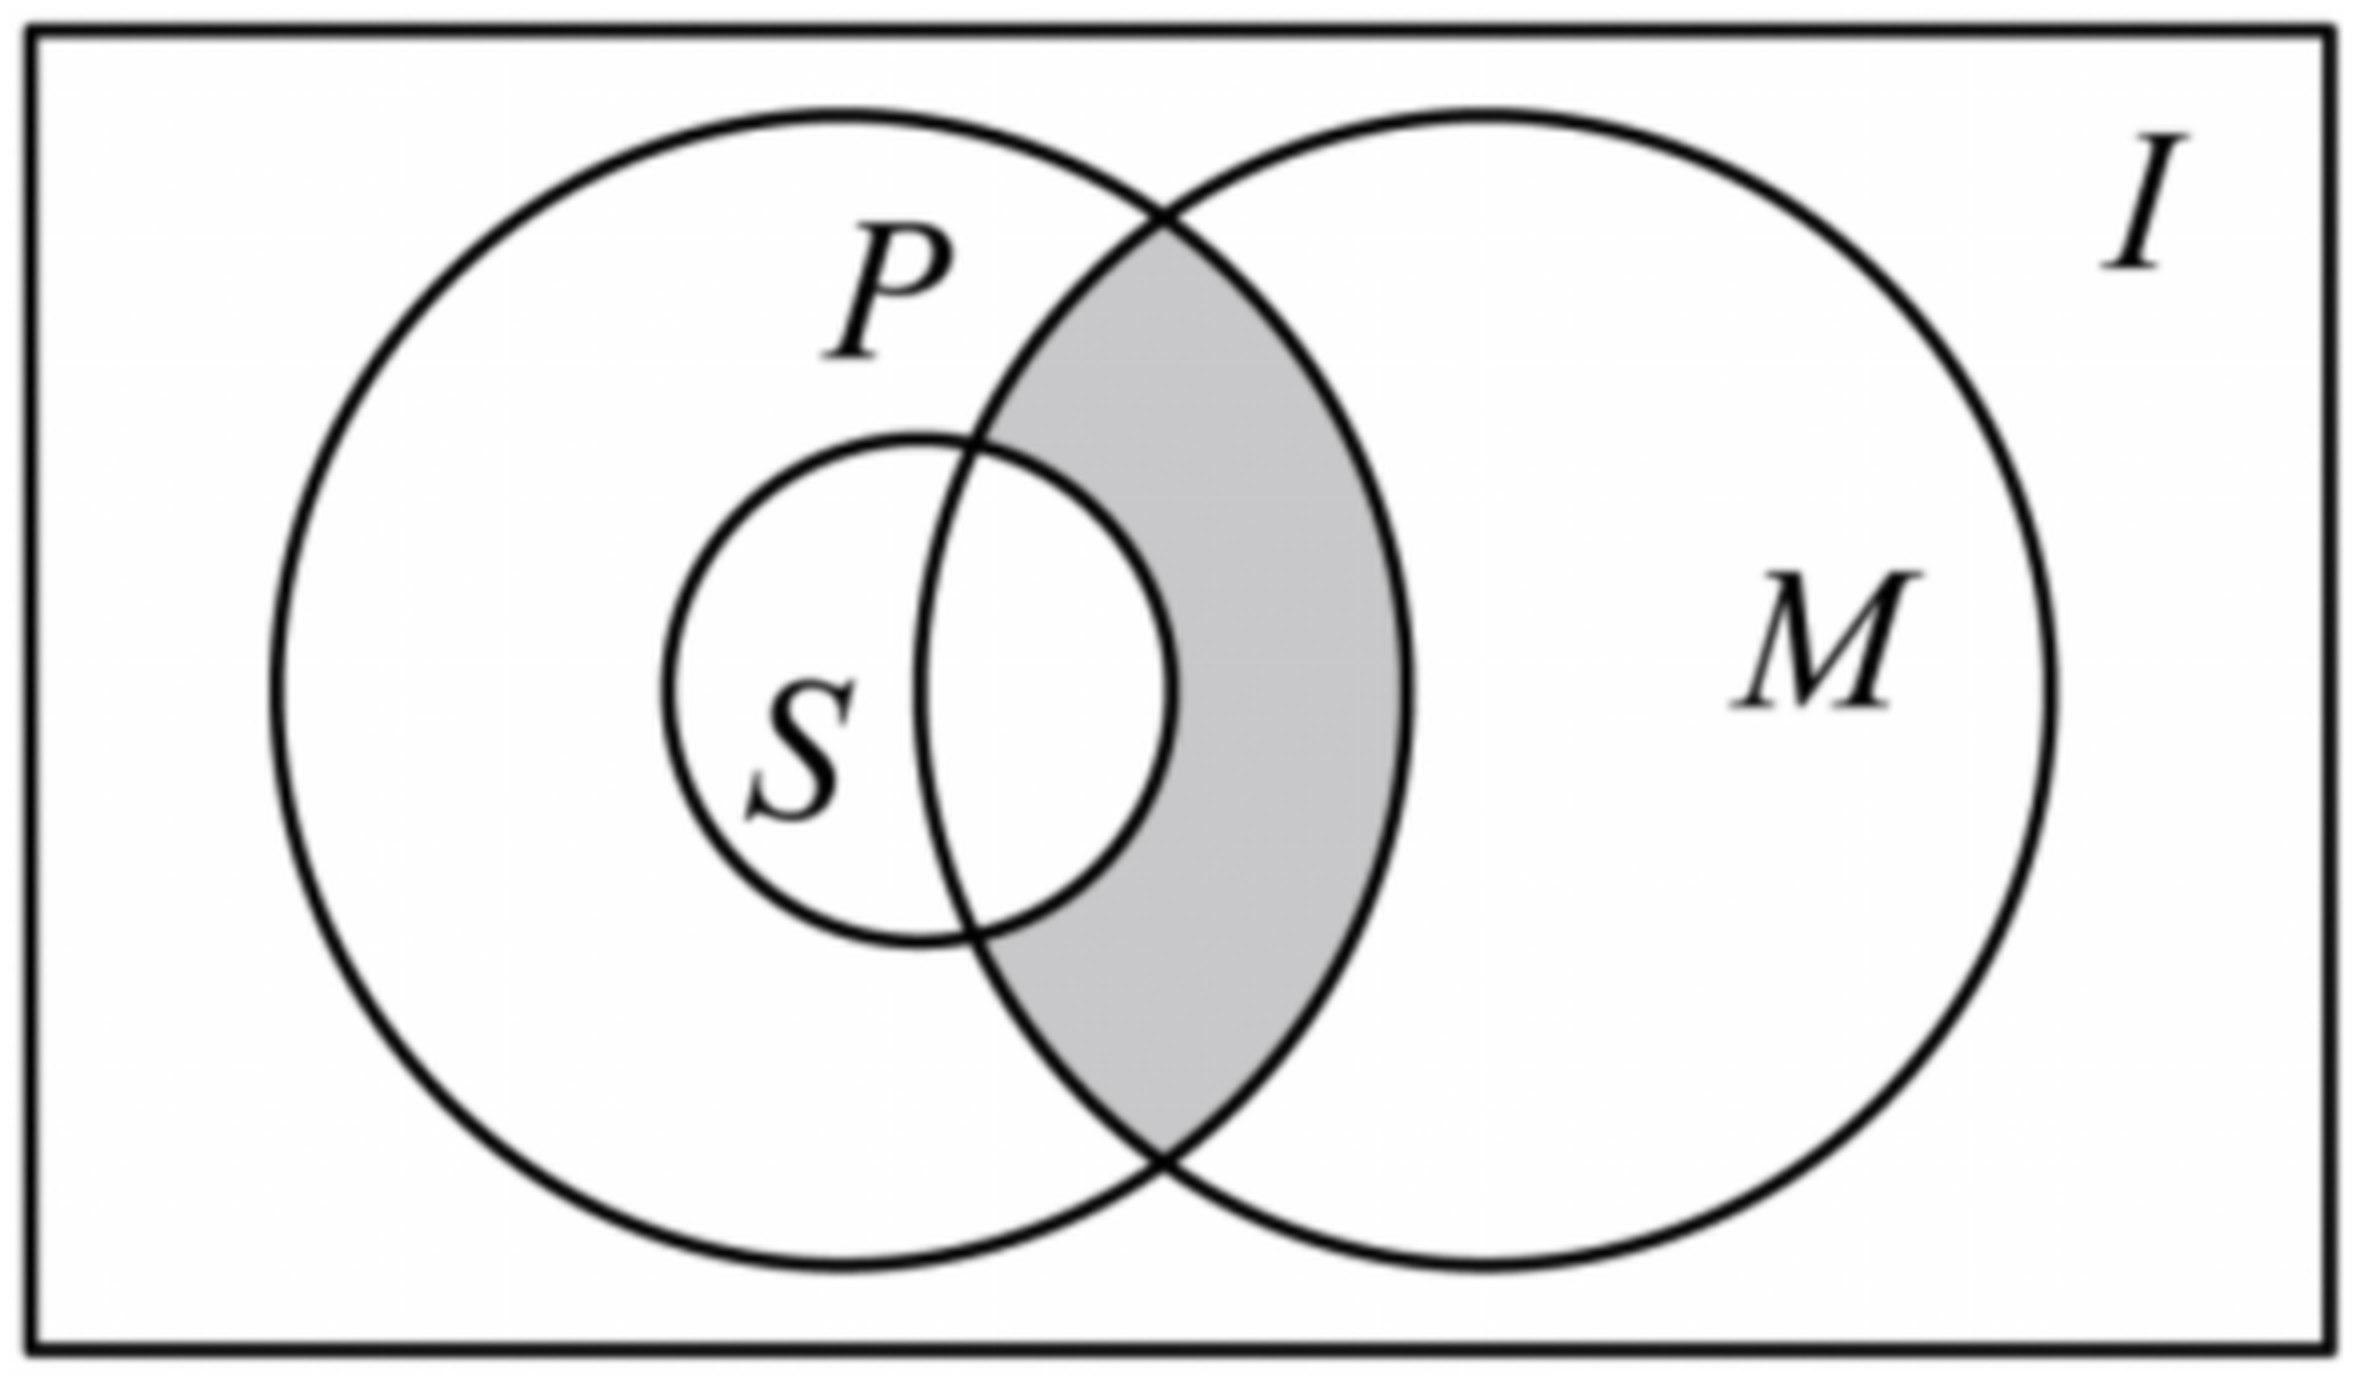
\includegraphics[width=0.46\textwidth]{figures/venn_MP_minus_S_h32.png}
\end{center}

\keepwithprev
A. $(M\cap P)\cap S$\qquad\qquad B. $(M\cap P)\cup S$

C. $(M\cap P)\cap\overline{S}$\qquad\qquad D. $(M\cap P)\cup\overline{S}$

\ans{$C$}

\ifanswer
\solbegin
\step{由 Venn 图得，集合表示 $M$、$P$ 的交集与 $S$ 的补集的交集，}
\step{即阴影部分所表示的集合是 $(M\cap P)\cap\overline{S}$. 故选 $C$.}
\solend

\fi

\item 若实数 $a$、$b$ 满足 $ab>0$，$a+2b=6$，则下列结论中错误的是\mbox{（\quad）}

\keepwithprev
A. $ab\leqslant\dfrac92$\qquad\qquad B. $a^2+4b^2\geqslant18$

C. $\dfrac1a+\dfrac2b$ 的最小值为 $\dfrac94$\qquad\qquad
D. $\dfrac{a^2}{a+1}+\dfrac{4b^2}{2b+1}$ 的最小值为 $\dfrac92$

\ans{$C$}

\ifanswer
\solbegin
\step{因为 $ab>0$，所以 $a$、$b$ 同号，又 $a+2b=6$，所以 $a$、$b$ 同正.}
\step{对于 $A$，由 $6=a+2b\geqslant2\sqrt{a\cdot2b}$ 得 $ab\leqslant\dfrac92$，故 $A$ 正确；}
\step{对于 $B$，由不等式 $\sqrt{\dfrac{m^2+n^2}2}\geqslant\dfrac{m+n}2$ 得
$\sqrt{\dfrac{a^2+(2b)^2}2}\geqslant\dfrac{a+2b}2=3$，}
\step{所以 $a^2+4b^2\geqslant18$，当且仅当 $a=2b=3$ 时取等号，故 $B$ 正确；}
\step{对于 $C$，$\dfrac1a+\dfrac2b
=\dfrac16\left(\dfrac1a+\dfrac2b\right)(a+2b)
=\dfrac16\left(5+\dfrac{2b}a+\dfrac{2a}b\right)$}
\step{$=\dfrac56+\dfrac13\left(\dfrac ba+\dfrac ab\right)
\geqslant\dfrac56+\dfrac13\times2\sqrt{\dfrac ba\cdot\dfrac ab}=\dfrac32$，}
\step{当且仅当 $\dfrac ba=\dfrac ab$，即 $a=b=2$ 时取等号，故 $C$ 错误；}
\step{对于 $D$，$\dfrac{a^2}{a+1}+\dfrac{4b^2}{2b+1}
=\dfrac{(a+1)^2-2(a+1)+1}{a+1}+\dfrac{(2b+1)^2-2(2b+1)+1}{2b+1}$}
\step{$=(a+1)-2+\dfrac1{a+1}+(2b+1)-2+\dfrac1{2b+1}
=(a+2b-2)+\dfrac1{a+1}+\dfrac1{2b+1}$}
\step{$=(6-2)+\dfrac{a+2b+2}{(a+1)(2b+1)}
=4+\dfrac8{(a+1)(2b+1)}$，}
\step{因为 $(a+1)(2b+1)\leqslant\left(\dfrac{a+1+2b+1}2\right)^2
=\left(\dfrac82\right)^2=16$，}
\step{当且仅当 $a+1=2b+1$，即 $a=2b=3$ 时取等号，}
\step{所以 $4+\dfrac8{(a+1)(2b+1)}\geqslant4+\dfrac8{16}=\dfrac92$，
故 $D$ 正确，其他几种方法同 12 题.}
\step{故选 $C$.}
\solend

\fi

% 注：本题的答案「D」原卷直接印在题干末尾的括号内，本稿按全稿惯例另提为 \ans{}。
\item 已知函数 $f(x)=x^2-2ax+a^2-1$，定义集合 $A=\{x\mid f(x)<0\}$. 若集合
$\{x\mid f(x)\in A\}=\varnothing$，则实数 $a$ 的取值范围是\mbox{（\quad）}

\keepwithprev
A. $(-3,-2)$\qquad B. $[-3,-2]$\qquad
C. $(-\infty,2)$\qquad D. $(-\infty,-2]$

\ans{$D$}

\item 非空集合 $A$ 具有如下性质：①若 $x$、$y\in A$，则 $\dfrac xy\in A$；
②若 $x$、$y\in A$，则 $x+y\in A$；

由此可知：下列判断中，错误的是\mbox{（\quad）}

\keepwithprev
A. $-1\notin A$\qquad\qquad B. $\dfrac{2025}{2026}\in A$

C. 若 $x$、$y\in A$，则 $xy\in A$\qquad\qquad
D. 若 $x$、$y\in A$，则 $x-y\in A$

\ans{$D$}

\ifanswer
\solbegin
\step{由题意得 $0\notin A$，$1\in A$，}
\step{对于 $A$，假设 $-1\in A$，则 $-1+1=0\in A$，矛盾，所以 $-1\notin A$，故 $A$ 正确；}
\step{对于 $B$，由 $1\in A$，得 $1+1=2\in A$，$2+1=3\in A$，…，$2025\in A$，$2026\in A$，}
\step{所以 $\dfrac{2025}{2026}\in A$，故 $B$ 正确；}
\step{对于 $C$，因为 $1\in A$，$x\in A$，所以 $\dfrac1x\in A$，
又因为 $y\in A$，所以 $\dfrac y{\frac1x}=xy\in A$，}
\step{故 $C$ 正确；}
\step{对于 $D$，因为 $1\in A$，$2\in A$，若 $x=1$，$y=2$，则 $x-y=-1\notin A$，故 $D$ 错误.}
\step{故选 $D$.}
\solend

\fi

\end{enumerate}

\bigsec{三、解答题}

\begin{enumerate}
\setcounter{enumi}{16}

\item 求下列关于实数 $x$ 的不等式的解集.

\begin{enumerate}[label=(\arabic*)]
\item $|2x+1|<5x-1$；
\item $\dfrac{(x-1)(x-3)(x-6)}{(x-2)(x-4)^2(x-5)}\geqslant0$.
\end{enumerate}

\ifanswer
\solbegin
\stepm{(1)}{因为不等式 $|2x+1|<5x-1$ 可化为 $-(5x-1)<2x+1<5x-1$，且 $5x-1>0$，}
\step{解得 $x>\dfrac23$，所以原不等式的解集为 $\left(\dfrac23,+\infty\right)$；}
\stepm{(2)}{不等式 $\dfrac{(x-1)(x-3)(x-6)}{(x-2)(x-4)^2(x-5)}\geqslant0$，}
\step{等价于 $(x-1)(x-3)(x-6)(x-2)(x-5)\geqslant0$，
且 $x-2\neq0$，$x-4\neq0$，$x-5\neq0$，}
\step{由“穿针引线法”，解得 $1\leqslant x<2$ 或 $3\leqslant x<4$ 或 $4<x<5$ 或 $x\geqslant6$，}
\step{所以不等式的解集为 $[1,2)\cup[3,4)\cup(4,5)\cup[6,+\infty)$.}
\solend

\fi

\ansspace[6]

\item 已知集合 $A=\left\{x\left|mx^2-mx+\dfrac{5m}2-6=0\right.\right\}\neq\varnothing$，
集合 $B=\{x\mid1<x<4$ 且 $x\in\Z\}$，$C=\{x\mid ax+3>0\}$；若 $A\cap B=A$.

\begin{enumerate}[label=(\arabic*)]
\item 求 $m$ 的取值范围.
\item 设 $m$ 的取值集合为 $D$，若 $C\cap D=\varnothing$，求 $m$ 的值及其对应 $a$ 的取值范围.
\end{enumerate}

\ans{略}

\ansspace[8]

\item 已知函数 $f(x)=x^2+(m-2)x+2m-1$.

\begin{enumerate}[label=(\arabic*)]
\item 若 $f(x)=0$ 的两根为 $x_1$、$x_2$，且 $|x_1-x_2|=2$，求实数 $m$ 的值；
\item 若函数 $y=f(x)$ 的图像在区间 $(0,1)$ 上与 $x$ 轴只有一个交点，
求实数 $m$ 的取值范围.
\end{enumerate}

\ifanswer
\solbegin
\stepm{(1)}{由题意得 $x_1+x_2=-(m-2)=2-m$，$x_1x_2=2m-1$，}
\step{由 $|x_1-x_2|=\sqrt{(x_1+x_2)^2-4x_1x_2}
=\sqrt{(2-m)^2-4(2m-1)}=2$，}
\step{化简得 $m^2-12m+4=0$，解得 $m=6\pm4\sqrt2$，故 $m=6\pm4\sqrt2$.}
\stepm{(2)}{当 $f(x)=0$ 只有一个根，且此根位于区间 $(0,1)$，}
\step{则 $\begin{cases}0<\dfrac{2-m}2<1\\[4pt]
\Delta=(m-2)^2-4(2m-1)=0\end{cases}$，
解得 $\begin{cases}0<m<2\\ m=6-2\sqrt7\text{ 或 }m=6+2\sqrt7\end{cases}$，}
\step{所以 $m=6-2\sqrt7$；}
\step{当 $f(x)=0$ 有两个根时，有一个根在区间 $(0,1)$ 内，且另一个根位于 $[0,1]$ 之外，}
\step{则 $\begin{cases}f(0)f(1)<0\\ \Delta=(m-2)^2-4(2m-1)>0\end{cases}$，
解得 $\begin{cases}\dfrac12<m<\dfrac23\\[4pt]
m<6-2\sqrt7\text{ 或 }m>6+2\sqrt7\end{cases}$，}
% 注：下一行原卷作「即 $\dfrac12<m<\dfrac32$」，按上一行方程组应为
%     $\dfrac12<m<\dfrac23$（同页最终答案也印证），照录未改，见文件头「原卷存疑」①。
\step{即 $\dfrac12<m<\dfrac32$；}
\step{当 $f(x)=0$ 有两个根位于区间 $[0,1]$ 内，且只有一个根在区间 $(0,1)$ 内，}
\step{则另一个根为 $0$ 时，得 $m=\dfrac12$，此时 $x_1+x_2=\dfrac32$，
解得另一个根 $x_2=\dfrac32>0$，故此种情况不符题意；}
\step{当 $f(x)=0$ 有两个根位于区间 $(0,1]$ 内，且只有一个根在区间 $(0,1)$ 内，}
\step{则另一个根为 $1$ 时，得 $m=\dfrac23$，此时 $x_1+x_2=\dfrac43$，
解得另一个根 $x_2=\dfrac13$，故此种情况符合题意；}
\step{综上所述，$m$ 的取值范围为
$\left(\dfrac12,\dfrac23\right]\cup\{6-2\sqrt7\}$.}
\solend

\fi

\ansspace[8]

\item 设集合 $A=\{a_1,a_2,a_3,a_4\}$，$B=\{b_1,b_2,b_3,b_4\}$，$C=\{2,3,4,6\}$，
新定义：集合 $A$ 中所有含 $k$ 个元素的子集中 $k$ 个元素之和组成的集合为“$k$ 元集和集”，
集合 $A$ 中所有含 $k$ 个元素的子集中最大元素减去剩余所有元素的和组成的集合为“$k$ 元差集”.

\begin{enumerate}[label=(\arabic*)]
\item 若 $A$ 的“$k$ 元集和集”为 $C$，求：集合 $A$.
\item 在 (1) 的条件下，若 $B$ 的“$k$ 元差集”为 $C$，求：所有满足条件的 $A\cap B$ 的真子集
个数之和.
\item 设 $b_1=a_1^2$，$b_2=a_2^2$，$b_3=a_3^2$，$b_4=a_4^2$，若 $A\cap B$ 为 $2$ 元集且
元素之和为 $10$ 且 $A$ 的“$2$ 元集和集”中最大元素不超过 $14$，求：所有满足条件的 $A$ 的
“$3$ 元差集”.
\end{enumerate}

\ifanswer
\solbegin
\stepm{(1)}{若 $A$ 的“$k$ 元集和集”为 $C$，$C=\{2,3,4,6\}$，则集合为 $\{-1,1,2,3\}$；}
\stepm{(2)}{$B$ 集合为 $\{5,3,0,-1\}$ 或 $\{9,3,1,0\}$ 或 $\{6,3,1,-1\}$，}
\step{故所有 $A\cap B$ 的真子集个数之和为 $13$；}
\stepm{(3)}{$b_1=a_1^2$，$b_2=a_2^2$，$b_3=a_3^2$，$b_4=a_4^2$，}
\step{若 $A\cap B$ 为 $2$ 元集且元素之和为 $10$，
且 $A$ 的“$2$ 元集和集”中最大元素不超过 $14$，}
% 注：下一行答案的第二个集合 $\{0,4,5,6\}$ 是 4 元集，而题问的却是「3 元差集」，
%     原卷如此，照录未改，见文件头「原卷存疑」③。
\step{则满足条件的 $A$ 的“$3$ 元差集” $\{1,3,5\}$ 或 $\{0,4,5,6\}$ 或 $\{2,4,5,8\}$.}
\solend

\fi

\ansspace[8]

\item 已知有限集 $X$、$Y$，定义集合 $X-Y=\{x\mid x\in X$ 且 $x\notin Y\}$，
$|X|$ 表示集合 $X$ 元素个数.

\begin{enumerate}[label=(\arabic*)]
\item 若 $X=\{1,2,3,4\}$，$Y=\{3,4,5\}$，写出集合 $X-Y$ 和 $Y-X$，以及
$|(X-Y)\cup(Y-X)|$ 的值；
\item 给定正整数 $n$，集合 $S=\{1,2,\cdots,n\}$，对于实数集的非空有限子集 $A$、$B$，
定义集合 $C=\{x\mid x=a+b,a\in A,b\in B\}$；

①求证：$|A-S|+|B-S|+|S-C|\geqslant1$；

②求 $|(A-S)\cup(S-A)|+|(B-S)\cup(S-B)|+|(C-S)\cup(S-C)|$ 的最小值.
\end{enumerate}

\ifanswer
\solbegin
\stepm{(1)}{由定义直接得 $X-Y=\{1,2\}$，$Y-X=\{5\}$，
$|(X-Y)\cup(Y-X)|=3$.}
% 注：下一句原卷作「显然 $|X|\geqslant0$」（按后文论证疑为 $|S|\geqslant0$），
%     照录未改，见文件头「原卷存疑」②。
\stepm{(2)}{①显然 $|X|\geqslant0$.}
\step{若 $A\cup B$ 中含有一个不在 $S$ 中的元素，则 $|A-S|+|B-S|\geqslant1$，
即 $|A-S|+|B-S|+|S-C|\geqslant1$.}
\step{若 $A\sub S$，且 $B\sub S$，则 $|A-S|=|B-S|=0$；}
\step{此时 $A$ 中最小的元素 $a\geqslant1$，$B$ 中最小的元素 $b\geqslant1$，
所以 $C$ 中最小的元素 $a+b\geqslant2$，所以 $1\notin C$.}
\step{因为 $S=\{1,2,\cdots,n\}$，所以 $|S-C|\geqslant1$，
即 $|A-S|+|B-S|+|S-C|\geqslant1$.}
\step{综上，$|A-S|+|B-S|+|S-C|\geqslant1$.}
\step{②由①得 $|A-S|+|B-S|+|S-C|\geqslant1$.}
\step{所以 $|(A-S)\cup(S-A)|+|(B-S)\cup(S-B)|+|(C-S)\cup(S-C)|$}
\step{$=|A-S|+|S-A|+|B-S|+|S-B|+|C-S|+|S-C|$}
\step{$\geqslant|S-A|+|S-B|+|C-S|+1$.}
\step{若 $A\cap S=\varnothing$，或 $B\cap S=\varnothing$，则 $|S-A|+|S-B|\geqslant n$.}
\step{若 $A\cap S\neq\varnothing$，且 $B\cap S\neq\varnothing$，
设 $A\cap S=\{a_1,a_2,\cdots,a_s\}$，$B\cap S=\{b_1,b_2,\cdots,b_t\}$，}
\step{且 $1\leqslant a_1<a_2<\cdots<a_s\leqslant n$，
$1\leqslant b_1<b_2<\cdots<b_t\leqslant n$，则 $|S-A|=n-s$，$|B-S|=n-t$.}
% 注：原卷的解析到此为止（第 10 页末），②的最小值并未给出，照录未补，
%     见文件头「原卷存疑」④。
\solend

\fi

\ansspace*[10]

\end{enumerate}

\end{document}
"
% 紧凑版：xelatex "\def\iscompact{1}% 高一32_华师大二附中_周末作业4.tex
%   —— 高一上数学「2026-2027 年华师大二附中高一上周末作业 4」（试卷版/答案版）
% 试卷版：xelatex 高一32_华师大二附中_周末作业4.tex
% 答案版：xelatex "\def\isanswer{1}\input{高一32_华师大二附中_周末作业4.tex}"
% 紧凑版：xelatex "\def\iscompact{1}\input{高一32_华师大二附中_周末作业4.tex}"
%
% 原始材料是微信公众号图文（公众号「魔都数学加油站」连载「27学年高一 32」，2026-09-25 发布，
% 原文标题「27学年高一32——2026-2027年上海市华师大二附中高一上周末作业4」），
% 正文为 10 张 PNG 页。**同一篇里各页分辨率不一致**（2560×3620 与 4762×6735 两档混排），
% 取 mmbiz.qpic.cn/<hash>/0 的原图档。原文本身就是一份**讲评版**——有的题下方印【解析】、
% 有的印【答案】，第 15 题的答案直接印在题干末尾的括号里。
% 试题文字、答案与解析均照原卷录入，未改内容。卷面的粉色斜水印属水印，未录入。
%
% ⚠ 卷首年份：本卷卷面印作「**2025-2026 年**」，与连载「27学年高一32」及公众号原文标题的
%   「2026-2027 年」**不一致**。经三人次分别把标题行裁出放大（4×—10×）独立判读，三次都读作
%   2025-2026，且校名作「华师大二附中」（无「东」字）、卷面亦无「上海市」三字。
%   按全稿「标题行照原卷」的口径，本稿照卷面排作「2025--2026 年…」——这是全稿唯一一份
%   年份不是 2026--2027 的卷子（其余 35 份均为 2026--2027）。
%
% 卷首标题：原卷印作「……年华师大二附中高一上周末作业 4」（公众号标题里的「上海市」
% 三字卷面标题行没有，本稿照卷面），年份区间按全稿惯例排 en dash，前缀照原卷保留「年」。
%
% 与原卷的排版差异（均已在 README「说明」中交代）：
%   ① 原文自**第 3 题**起（第 1、2 题未在该文中发布），故本稿题号亦自 3 起；
%   ② 原卷本就印有「一、填空题」「二、选择题」「三、解答题」三节标题，本稿照原卷分节，
%      只把标题改排成全稿统一的「大节标题」样式；
%   ③ 原卷第 6、8、9 题只印【答案】行（第 18 题的【答案】印作「略”），其余各题印【解析】，
%      第 15 题的答案直接印在题干末尾的括号内；本稿统一改为试卷版隐去、
%      答案版以 \ans{}／\ifanswer 块给出，两版彻底分离；
%   ④ 子集符号原卷两种并用：第 21(2)① 的 $A\sub S$、$B\sub S$ 带下划线，
%      第 3、10 题的 $(0,2)\subset(-\infty,3)$、$A\subset B$、$\overline{B}\subset\overline{A}$
%      作真包含，本稿分别照录为 $\sub$ 与 $\subset$；
%   ⑤ 补集符号原卷一律作上横线（$\overline{A}$、$\overline{B}$、$\overline{S}$），本稿照录；
%      空集原卷作「斜杠伸出圆外」的 $\varnothing$；
%   ⑥ 判别式记号原卷两种：第 4 题作粗体的 $\Delta$、第 11 题作细等宽的 $\triangle$，本稿照录；
%   ⑦ 数集记号原卷作斜体的 $R$、$Z$（第 4、18 题），本稿按全稿惯例统一写作 $\R$、$\Z$；
%   ⑧ 原卷填空的横线约两个字宽，本稿按全稿惯例统一排 \blankline[4.4em]；
%   ⑨ 原卷未印副标题，本稿按全稿惯例补出副标题「集合与常用逻辑用语」；
%   ⑩ 本卷只有第 13 题一图（韦恩图），原卷印在题干右侧，本稿移至题干之后；
%      图取原卷截图、4× LANCZOS 放大（figures/venn_MP_minus_S_h32.png）。
%
% 原卷存疑四处（均照抄原卷、未改，见源码中该处上方注释）：
%   ① 第 19(2)【解析】有「即 $\dfrac12<m<\dfrac32$」，按上一行的方程组应为
%      $\dfrac12<m<\dfrac23$（同页最终答案 $\left(\dfrac12,\dfrac23\right]$ 也印证）；
%   ② 第 21(2)① 首句作「显然 $|X|\geqslant0$」（按后文论证疑为 $|S|\geqslant0$）；
%   ③ 第 20(3) 的答案第二个集合 $\{0,4,5,6\}$ 是 4 元集，而题问的是「3 元差集」；
%   ④ 第 21(2)② 的解析**原卷就未写完**（第 10 页到「则 $|S-A|=n-s$，$|B-S|=n-t$」即止）。

\documentclass[a4paper,11pt]{article}
\usepackage{common}

\begin{document}

\examtitlest[3]{2025--2026 年华师大二附中高一上周末作业 4}{集合与常用逻辑用语}

\bigsec{一、填空题}

\begin{enumerate}
\setcounter{enumi}{2}

\item 设 $x$ 为实数，则“$x<3$”是“$x(x-2)<0$”的 \blankline[4.4em] 条件.

\ifanswer
\solbegin
\step{$x(x-2)<0$，解得 $0<x<2$，$(0,2)\subset(-\infty,3)$，}
\step{若 $x$ 属于“$x(x-2)<0$”，则属于“$x<3$”一定成立，即满足必要性，}
\step{若 $x$ 属于“$x<3$”，不一定满足“$x(x-2)<0$”，如 $x=-1$，即充分性不成立；}
\step{故“$x<3$”是“$x(x-2)<0$”的必要不充分条件.}
\solend

\fi

\item 若关于 $x$ 的不等式 $kx^2-kx+1>0$ 的解集为 $\R$，则实数 $k$ 的取值范围为
\blankline[4.4em].

\ifanswer
\solbegin
\step{①当 $k=0$ 时，不等式为 $1>0$ 恒成立，满足题意；}
\step{②当 $k\neq0$ 时，只要 $\begin{cases}k>0\\ \Delta=k^2-4k<0\end{cases}$，
解得 $0<k<4$；}
\step{所以不等式 $kx^2-kx+1>0$ 的解集为 $\R$，则实数 $k$ 的取值范围为 $[0,4)$.}
\solend

\fi

\item 已知 $1<a<3$，$-5<b<-2$，则 $\dfrac ab$ 的取值范围是 \blankline[4.4em].

\ifanswer
\solbegin
\step{因为 $-5<b<-2$，所以 $2<-b<5$，$\dfrac15<-\dfrac1b<\dfrac12$，又 $1<a<3$，}
\step{得 $\dfrac15<-\dfrac ab<\dfrac32$，则 $-\dfrac32<\dfrac ab<-\dfrac15$，
故 $\dfrac ab$ 的取值范围是 $\left(-\dfrac32,-\dfrac15\right)$.}
\solend

\fi

\item 关于 $x$ 的不等式 $\dfrac{ax-1}{x-a}>1$ 的解集为 $A$，且 $3\notin A$，
则实数 $a$ 的取值范围为 \blankline[4.4em].

\ans{$(-\infty,1]\cup[3,+\infty)$}

\item 若关于 $x$ 的不等式 $a\leqslant\dfrac34x^2-3x+4\leqslant b$ 的解集恰好是 $[a,b]$，
则 $b-a=$ \blankline[4.4em].

\ifanswer
\solbegin
\step{令 $f(x)=\dfrac34x^2-3x+4$，则 $f(x)$ 的对称轴为 $x=2$，}
\step{画出函数 $f(x)=\dfrac34x^2-3x+4=\dfrac34(x-2)^2+1$ 的图象，
得 $f(x)_{\min}=f(2)=1$，}
\step{由题意得 $a\leqslant1$，且 $f(a)=f(b)=b$，$a<b$，}
\step{由 $f(b)=b$ 得 $\dfrac34b^2-3b+4=b$，解得 $b=\dfrac43$（舍去）或 $b=4$，得 $b=4$，}
\step{由抛物线的对称轴为 $x=2$ 得 $a=0$，所以 $b-a=4$.}
\solend

\fi

\item 若关于 $x$ 的方程 $x^2-2kx+k+4=0$ 在 $[1,2]$ 上有解，则实数 $k$ 的取值范围为
\blankline[4.4em].

\ans{$\left[\dfrac83,5\right]$}

\item 记关于 $x$ 的方程 $x^2-2mx-2m+3=0$ 的两实根为 $x_1$、$x_2$，
则 $(x_1-2)^2+(x_2-2)^2$ 的最小值为 \blankline[4.4em].

\ans{$2$}

\item 若“$|mx^2-4x+3|\geqslant2$”的必要非充分条件是“$x\leqslant1$ 或 $x\geqslant4$”，
则实数 $m$ 的取值范围是 \blankline[4.4em].

\ifanswer
\solbegin
\step{记 $|mx^2-4x+3|\geqslant2$ 的解集为集合 $A$，
$B=\{x\mid x\leqslant1\text{ 或 }x\geqslant4\}$，}
\step{则 $\overline{A}$ 为 $|mx^2-4x+3|<2$ 的解集，$\overline{B}=\{x\mid1<x<4\}$；}
\step{因为 $B$ 是 $A$ 的必要非充分条件，所以 $A\subset B$，
得 $\overline{B}\subset\overline{A}$，}
\step{即对任意 $x\in(1,4)$，都有 $|mx^2-4x+3|<2$ 恒成立.}
\step{因为 $|mx^2-4x+3|<2$，$1<x<4$，所以 $-2<mx^2-4x+3<2$，}
\step{化简得
$-5\left(\dfrac1x\right)^2+4\left(\dfrac1x\right)
<m<-\left(\dfrac1x\right)^2+4\left(\dfrac1x\right)$；}
\step{令 $t=\dfrac1x$，$g(t)=-5t^2+4t$，$h(t)=-t^2+4t$，
且 $t\in\left(\dfrac14,1\right)$；}
\step{所以 $g(t)=-5t^2+4t=-5\left(t-\dfrac25\right)^2+\dfrac45$，
当 $t=\dfrac25$ 时，$g(t)$ 取得最大值 $\dfrac45$，}
\step{$h(t)=-t^2+4t=-(t-2)^2+4$，当 $t=\dfrac14$ 时，$h(t)$ 取得最小值，
即 $h(t)>h\left(\dfrac14\right)=\dfrac{15}{16}$；}
\step{因为对任意 $t\in\left(\dfrac14,1\right)$，$g(t)<m<h(t)$ 恒成立，
所以 $g\left(\dfrac25\right)<m\leqslant h\left(\dfrac14\right)$，}
\step{即 $\dfrac45<m\leqslant\dfrac{15}{16}$，
所以 $m$ 的取值范围是 $\left(\dfrac45,\dfrac{15}{16}\right]$.}
\solend

\fi

\item 已知关于 $x$ 的方程 $x^2+2(m-2)x+m^2-3m+3=0$ 有两个不相等的实数根 $x_1$、$x_2$，则

$\dfrac{mx_1}{x_1-1}+\dfrac{mx_2}{x_2-1}-\dfrac2{x_1+x_2-2}$ 的最大值为 \blankline[4.4em].

\ifanswer
\solbegin
\step{关于 $x$ 的方程 $x^2+2(m-2)x+m^2-3m+3=0$ 有两个不相等的实数根 $x_1$、$x_2$，}
\step{则 $\triangle=4(m-2)^2-4(m^2-3m+3)=-4m+4>0$，得 $m<1$，}
\step{且 $x_1+x_2=-2(m-2)$，$x_1x_2=m^2-3m+3$，}
\step{$\dfrac{mx_1}{x_1-1}+\dfrac{mx_2}{x_2-1}-\dfrac2{x_1+x_2-2}
=\dfrac{m[2x_1x_2-(x_1+x_2)]}{x_1x_2-(x_1+x_2)+1}+\dfrac1{m-1}$}
\step{$=\dfrac{2m(m-1)^2}{m^2-m}+\dfrac1{m-1}=2(m-1)+\dfrac1{m-1}$，}
\step{又因为 $m<1$，所以 $m-1<0$，则 $1-m>0$，}
\step{所以 $2(1-m)+\dfrac1{1-m}\geqslant2\sqrt{2(1-m)\cdot\dfrac1{1-m}}=2\sqrt2$，}
\step{当且仅当 $2(1-m)=\dfrac1{1-m}$ 时，即 $m=1-\dfrac{\sqrt2}2$ 时取等号，}
\step{所以 $2(m-1)+\dfrac1{m-1}\leqslant-2\sqrt2$，
即 $\dfrac{mx_1}{x_1-1}+\dfrac{mx_2}{x_2-1}-\dfrac2{x_1+x_2-2}$ 的最大值为 $-2\sqrt2$.}
\solend

\fi

\item 若正实数 $a$、$b$ 满足 $a+2b=ab$，则 $\dfrac4{a^2+2a}+\dfrac1{2b^2+b}$ 的最小值是
\blankline[4.4em].

\ifanswer
\solbegin
\stepm{法一}{由 $a+2b=ab$，得 $\dfrac2a+\dfrac1b=1$，}
\step{令 $x=\dfrac1a$，$y=\dfrac1b$，则 $x$、$y>0$，$2x+y=1$，$2x+1+y+2=4$，}
\step{所以 $\dfrac4{a^2+2a}+\dfrac1{2b^2+b}
=\dfrac4{\frac1{x^2}+\frac2x}+\dfrac1{\frac2{y^2}+\frac1y}
=\dfrac{4x^2}{2x+1}+\dfrac{y^2}{y+2}$（*）}
\step{$=\dfrac{(2x+1)^2-2(2x+1)+1}{2x+1}+\dfrac{(y+2)^2-4(y+2)+4}{y+2}$}
\step{$=2x-1+\dfrac1{2x+1}+y-2+\dfrac4{y+2}=\dfrac1{2x+1}+\dfrac4{y+2}-2$}
\step{$=\dfrac14\left(\dfrac1{2x+1}+\dfrac4{y+2}\right)(2x+1+y+2)-2$}
\step{$=\dfrac14\left[5+\dfrac{y+2}{2x+1}+\dfrac{4(2x+1)}{y+2}\right]-2
\geqslant\dfrac14(5+2\sqrt4)-2=\dfrac14$，}
\step{当且仅当 $\dfrac{y+2}{2x+1}=\dfrac{4(2x+1)}{y+2}$，
即 $x=\dfrac16$，$y=\dfrac23$ 时取等号，}
\step{故 $\dfrac4{a^2+2a}+\dfrac1{2b^2+b}$ 的最小值是 $\dfrac14$.}
\stepm{法二}{在法一（*）后，由权方和不等式，得
$\dfrac4{a^2+2a}+\dfrac1{2b^2+b}
=\dfrac{4x^2}{2x+1}+\dfrac{y^2}{y+2}
\geqslant\dfrac{(2x+y)^2}{2x+1+y+2}=\dfrac14$，}
\step{当且仅当……，故 $\dfrac4{a^2+2a}+\dfrac1{2b^2+b}$ 的最小值是 $\dfrac14$.}
\stepm{法三}{注意到
$\left(\dfrac{a+2}a+\dfrac{2b+1}b\right)\left(\dfrac4{a^2+2a}+\dfrac1{2b^2+b}\right)$}
\step{$\geqslant
\left(\sqrt{\dfrac{a+2}a\cdot\dfrac4{a^2+2a}}
+\sqrt{\dfrac{2b+1}b\cdot\dfrac1{2b^2+b}}\right)^2
=\left(\dfrac2a+\dfrac1b\right)^2$，}
\step{其中 $\dfrac{a+2}a+\dfrac{2b+1}b=3+\dfrac{a+2b}{ab}=4$，
$\dfrac2a+\dfrac1b=\dfrac{a+2b}{ab}=1$，}
\step{所以 $\dfrac4{a^2+2a}+\dfrac1{2b^2+b}\geqslant\dfrac14$，
当且仅当……，故 $\dfrac4{a^2+2a}+\dfrac1{2b^2+b}$ 的最小值是 $\dfrac14$.}
\solend

\fi

\end{enumerate}

\bigsec{二、选择题}

\begin{enumerate}
\setcounter{enumi}{12}

\item 如图，$I$ 为全集，$M$、$P$、$S$ 是 $I$ 的三个子集，则阴影部分所表示的集合是
\mbox{（\quad）}

\begin{center}
% 图取原卷截图、4× LANCZOS 放大（原卷把图印在题干右侧，本稿移至此处，见文件头⑩）。
% 矩形为全集 $I$，左大圆 $P$（内下方含小圆 $S$，其右侧伸入 $P$ 与 $M$ 的重叠区）、
% 右大圆 $M$；阴影是 $P$、$M$ 重叠的透镜形区域挖掉 $S$ 后剩下的部分（左缘呈弯月形）。
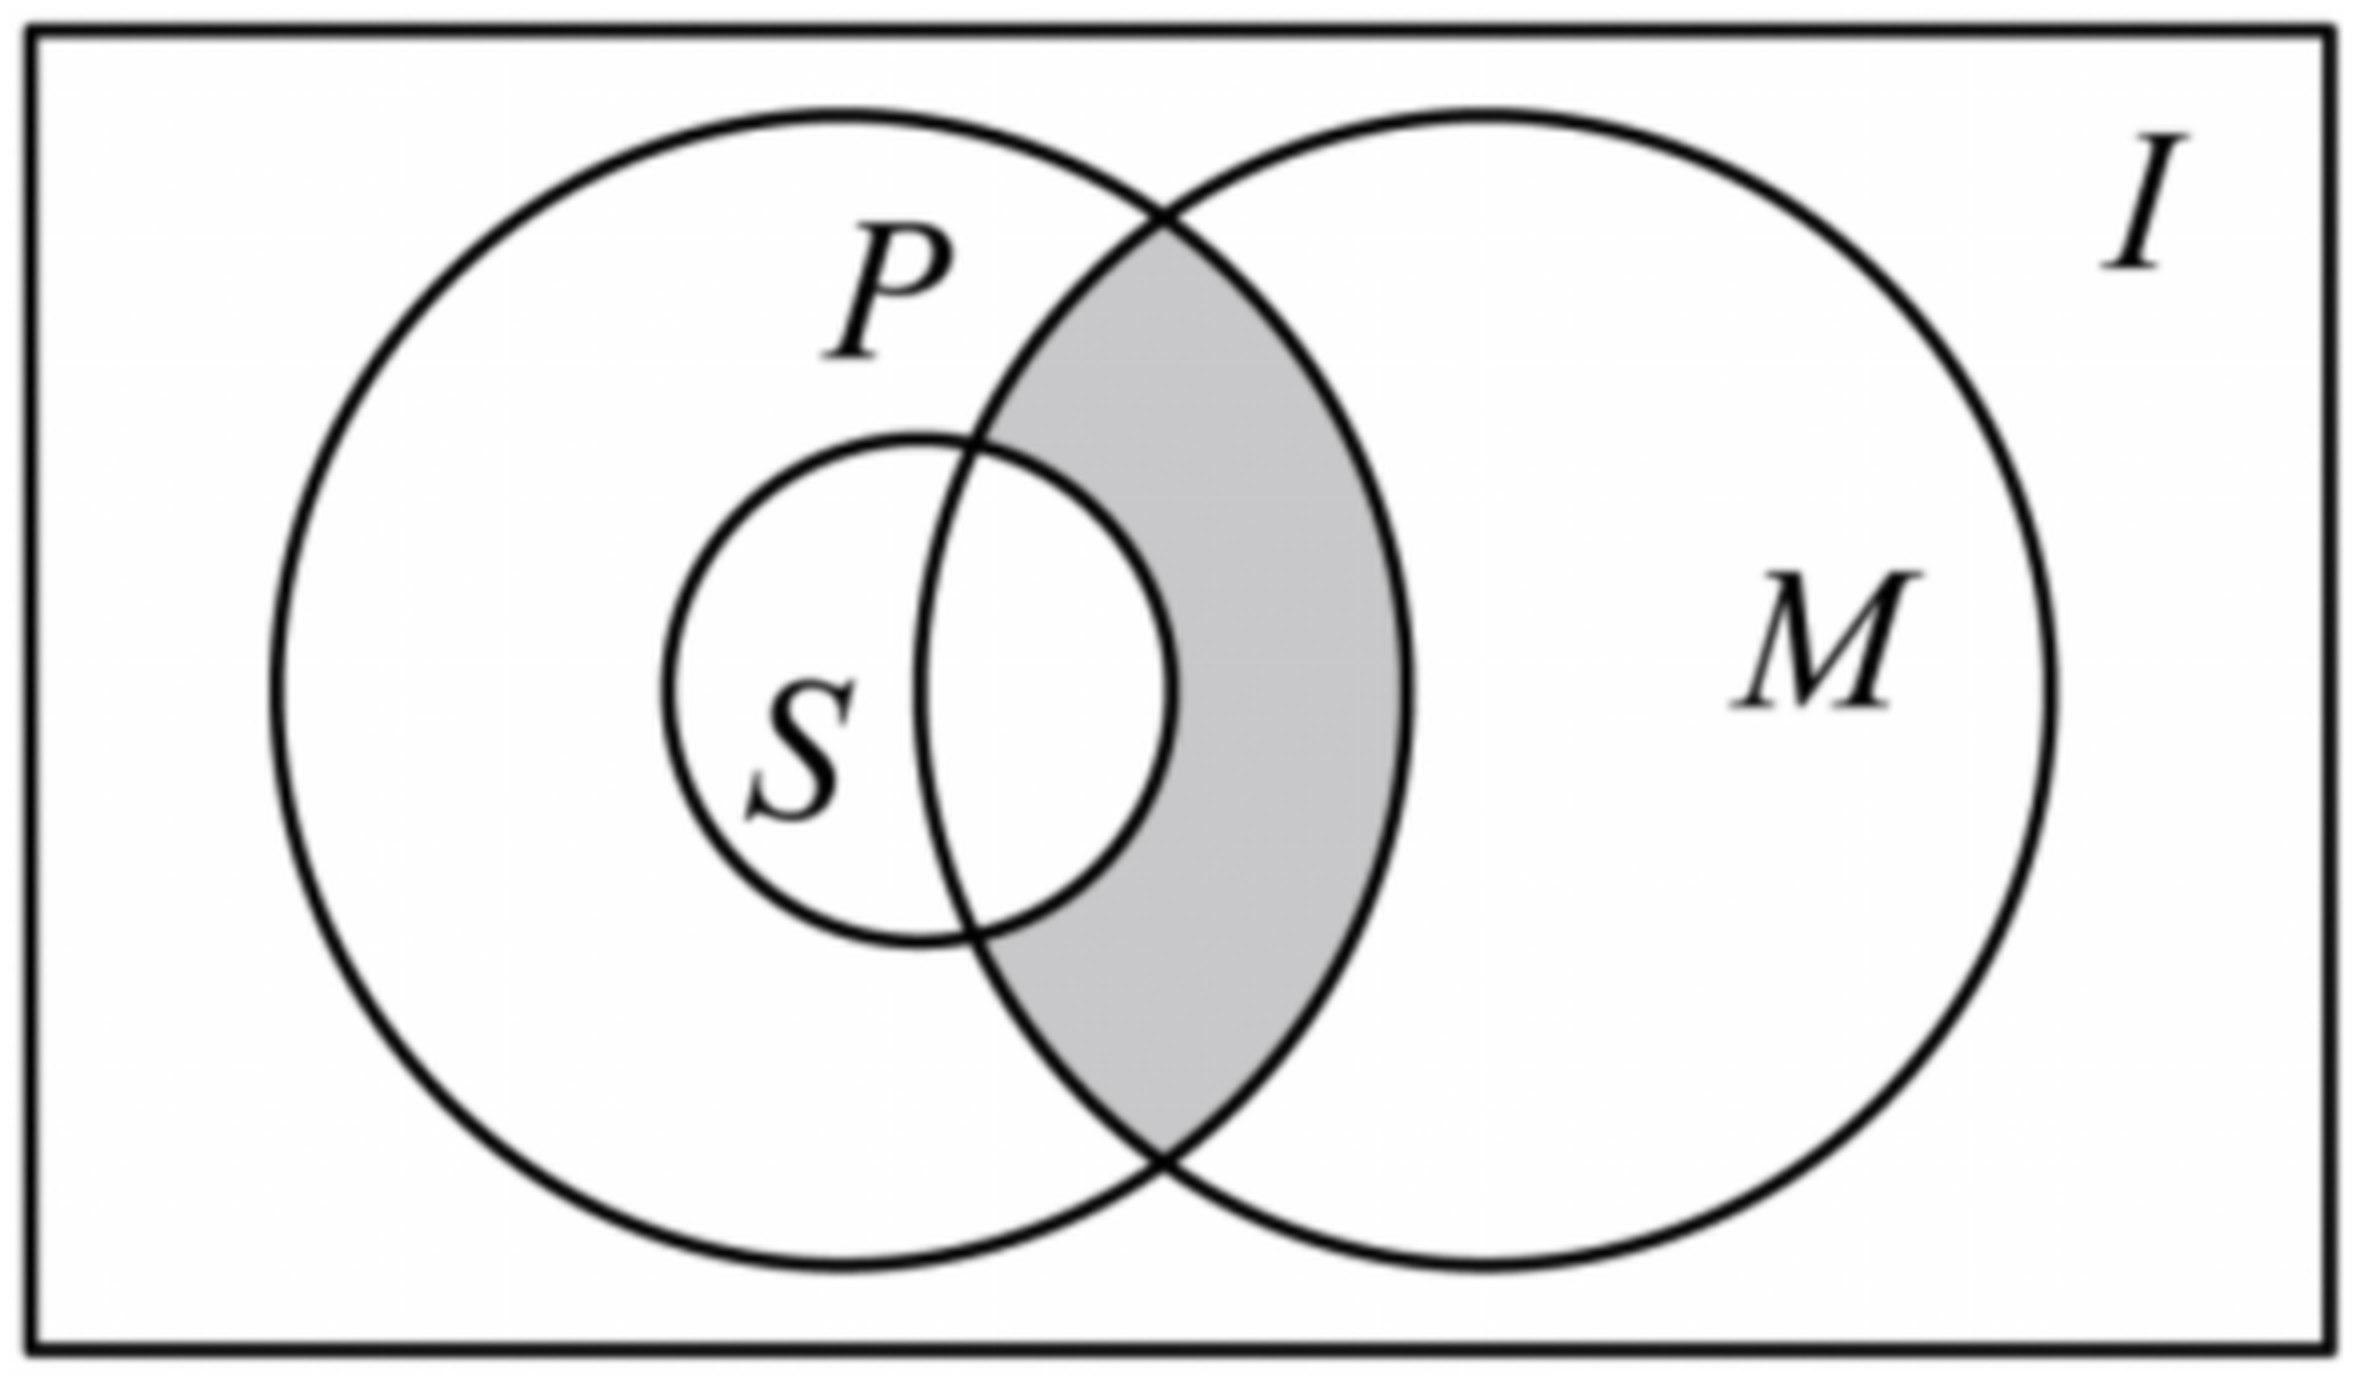
\includegraphics[width=0.46\textwidth]{figures/venn_MP_minus_S_h32.png}
\end{center}

\keepwithprev
A. $(M\cap P)\cap S$\qquad\qquad B. $(M\cap P)\cup S$

C. $(M\cap P)\cap\overline{S}$\qquad\qquad D. $(M\cap P)\cup\overline{S}$

\ans{$C$}

\ifanswer
\solbegin
\step{由 Venn 图得，集合表示 $M$、$P$ 的交集与 $S$ 的补集的交集，}
\step{即阴影部分所表示的集合是 $(M\cap P)\cap\overline{S}$. 故选 $C$.}
\solend

\fi

\item 若实数 $a$、$b$ 满足 $ab>0$，$a+2b=6$，则下列结论中错误的是\mbox{（\quad）}

\keepwithprev
A. $ab\leqslant\dfrac92$\qquad\qquad B. $a^2+4b^2\geqslant18$

C. $\dfrac1a+\dfrac2b$ 的最小值为 $\dfrac94$\qquad\qquad
D. $\dfrac{a^2}{a+1}+\dfrac{4b^2}{2b+1}$ 的最小值为 $\dfrac92$

\ans{$C$}

\ifanswer
\solbegin
\step{因为 $ab>0$，所以 $a$、$b$ 同号，又 $a+2b=6$，所以 $a$、$b$ 同正.}
\step{对于 $A$，由 $6=a+2b\geqslant2\sqrt{a\cdot2b}$ 得 $ab\leqslant\dfrac92$，故 $A$ 正确；}
\step{对于 $B$，由不等式 $\sqrt{\dfrac{m^2+n^2}2}\geqslant\dfrac{m+n}2$ 得
$\sqrt{\dfrac{a^2+(2b)^2}2}\geqslant\dfrac{a+2b}2=3$，}
\step{所以 $a^2+4b^2\geqslant18$，当且仅当 $a=2b=3$ 时取等号，故 $B$ 正确；}
\step{对于 $C$，$\dfrac1a+\dfrac2b
=\dfrac16\left(\dfrac1a+\dfrac2b\right)(a+2b)
=\dfrac16\left(5+\dfrac{2b}a+\dfrac{2a}b\right)$}
\step{$=\dfrac56+\dfrac13\left(\dfrac ba+\dfrac ab\right)
\geqslant\dfrac56+\dfrac13\times2\sqrt{\dfrac ba\cdot\dfrac ab}=\dfrac32$，}
\step{当且仅当 $\dfrac ba=\dfrac ab$，即 $a=b=2$ 时取等号，故 $C$ 错误；}
\step{对于 $D$，$\dfrac{a^2}{a+1}+\dfrac{4b^2}{2b+1}
=\dfrac{(a+1)^2-2(a+1)+1}{a+1}+\dfrac{(2b+1)^2-2(2b+1)+1}{2b+1}$}
\step{$=(a+1)-2+\dfrac1{a+1}+(2b+1)-2+\dfrac1{2b+1}
=(a+2b-2)+\dfrac1{a+1}+\dfrac1{2b+1}$}
\step{$=(6-2)+\dfrac{a+2b+2}{(a+1)(2b+1)}
=4+\dfrac8{(a+1)(2b+1)}$，}
\step{因为 $(a+1)(2b+1)\leqslant\left(\dfrac{a+1+2b+1}2\right)^2
=\left(\dfrac82\right)^2=16$，}
\step{当且仅当 $a+1=2b+1$，即 $a=2b=3$ 时取等号，}
\step{所以 $4+\dfrac8{(a+1)(2b+1)}\geqslant4+\dfrac8{16}=\dfrac92$，
故 $D$ 正确，其他几种方法同 12 题.}
\step{故选 $C$.}
\solend

\fi

% 注：本题的答案「D」原卷直接印在题干末尾的括号内，本稿按全稿惯例另提为 \ans{}。
\item 已知函数 $f(x)=x^2-2ax+a^2-1$，定义集合 $A=\{x\mid f(x)<0\}$. 若集合
$\{x\mid f(x)\in A\}=\varnothing$，则实数 $a$ 的取值范围是\mbox{（\quad）}

\keepwithprev
A. $(-3,-2)$\qquad B. $[-3,-2]$\qquad
C. $(-\infty,2)$\qquad D. $(-\infty,-2]$

\ans{$D$}

\item 非空集合 $A$ 具有如下性质：①若 $x$、$y\in A$，则 $\dfrac xy\in A$；
②若 $x$、$y\in A$，则 $x+y\in A$；

由此可知：下列判断中，错误的是\mbox{（\quad）}

\keepwithprev
A. $-1\notin A$\qquad\qquad B. $\dfrac{2025}{2026}\in A$

C. 若 $x$、$y\in A$，则 $xy\in A$\qquad\qquad
D. 若 $x$、$y\in A$，则 $x-y\in A$

\ans{$D$}

\ifanswer
\solbegin
\step{由题意得 $0\notin A$，$1\in A$，}
\step{对于 $A$，假设 $-1\in A$，则 $-1+1=0\in A$，矛盾，所以 $-1\notin A$，故 $A$ 正确；}
\step{对于 $B$，由 $1\in A$，得 $1+1=2\in A$，$2+1=3\in A$，…，$2025\in A$，$2026\in A$，}
\step{所以 $\dfrac{2025}{2026}\in A$，故 $B$ 正确；}
\step{对于 $C$，因为 $1\in A$，$x\in A$，所以 $\dfrac1x\in A$，
又因为 $y\in A$，所以 $\dfrac y{\frac1x}=xy\in A$，}
\step{故 $C$ 正确；}
\step{对于 $D$，因为 $1\in A$，$2\in A$，若 $x=1$，$y=2$，则 $x-y=-1\notin A$，故 $D$ 错误.}
\step{故选 $D$.}
\solend

\fi

\end{enumerate}

\bigsec{三、解答题}

\begin{enumerate}
\setcounter{enumi}{16}

\item 求下列关于实数 $x$ 的不等式的解集.

\begin{enumerate}[label=(\arabic*)]
\item $|2x+1|<5x-1$；
\item $\dfrac{(x-1)(x-3)(x-6)}{(x-2)(x-4)^2(x-5)}\geqslant0$.
\end{enumerate}

\ifanswer
\solbegin
\stepm{(1)}{因为不等式 $|2x+1|<5x-1$ 可化为 $-(5x-1)<2x+1<5x-1$，且 $5x-1>0$，}
\step{解得 $x>\dfrac23$，所以原不等式的解集为 $\left(\dfrac23,+\infty\right)$；}
\stepm{(2)}{不等式 $\dfrac{(x-1)(x-3)(x-6)}{(x-2)(x-4)^2(x-5)}\geqslant0$，}
\step{等价于 $(x-1)(x-3)(x-6)(x-2)(x-5)\geqslant0$，
且 $x-2\neq0$，$x-4\neq0$，$x-5\neq0$，}
\step{由“穿针引线法”，解得 $1\leqslant x<2$ 或 $3\leqslant x<4$ 或 $4<x<5$ 或 $x\geqslant6$，}
\step{所以不等式的解集为 $[1,2)\cup[3,4)\cup(4,5)\cup[6,+\infty)$.}
\solend

\fi

\ansspace[6]

\item 已知集合 $A=\left\{x\left|mx^2-mx+\dfrac{5m}2-6=0\right.\right\}\neq\varnothing$，
集合 $B=\{x\mid1<x<4$ 且 $x\in\Z\}$，$C=\{x\mid ax+3>0\}$；若 $A\cap B=A$.

\begin{enumerate}[label=(\arabic*)]
\item 求 $m$ 的取值范围.
\item 设 $m$ 的取值集合为 $D$，若 $C\cap D=\varnothing$，求 $m$ 的值及其对应 $a$ 的取值范围.
\end{enumerate}

\ans{略}

\ansspace[8]

\item 已知函数 $f(x)=x^2+(m-2)x+2m-1$.

\begin{enumerate}[label=(\arabic*)]
\item 若 $f(x)=0$ 的两根为 $x_1$、$x_2$，且 $|x_1-x_2|=2$，求实数 $m$ 的值；
\item 若函数 $y=f(x)$ 的图像在区间 $(0,1)$ 上与 $x$ 轴只有一个交点，
求实数 $m$ 的取值范围.
\end{enumerate}

\ifanswer
\solbegin
\stepm{(1)}{由题意得 $x_1+x_2=-(m-2)=2-m$，$x_1x_2=2m-1$，}
\step{由 $|x_1-x_2|=\sqrt{(x_1+x_2)^2-4x_1x_2}
=\sqrt{(2-m)^2-4(2m-1)}=2$，}
\step{化简得 $m^2-12m+4=0$，解得 $m=6\pm4\sqrt2$，故 $m=6\pm4\sqrt2$.}
\stepm{(2)}{当 $f(x)=0$ 只有一个根，且此根位于区间 $(0,1)$，}
\step{则 $\begin{cases}0<\dfrac{2-m}2<1\\[4pt]
\Delta=(m-2)^2-4(2m-1)=0\end{cases}$，
解得 $\begin{cases}0<m<2\\ m=6-2\sqrt7\text{ 或 }m=6+2\sqrt7\end{cases}$，}
\step{所以 $m=6-2\sqrt7$；}
\step{当 $f(x)=0$ 有两个根时，有一个根在区间 $(0,1)$ 内，且另一个根位于 $[0,1]$ 之外，}
\step{则 $\begin{cases}f(0)f(1)<0\\ \Delta=(m-2)^2-4(2m-1)>0\end{cases}$，
解得 $\begin{cases}\dfrac12<m<\dfrac23\\[4pt]
m<6-2\sqrt7\text{ 或 }m>6+2\sqrt7\end{cases}$，}
% 注：下一行原卷作「即 $\dfrac12<m<\dfrac32$」，按上一行方程组应为
%     $\dfrac12<m<\dfrac23$（同页最终答案也印证），照录未改，见文件头「原卷存疑」①。
\step{即 $\dfrac12<m<\dfrac32$；}
\step{当 $f(x)=0$ 有两个根位于区间 $[0,1]$ 内，且只有一个根在区间 $(0,1)$ 内，}
\step{则另一个根为 $0$ 时，得 $m=\dfrac12$，此时 $x_1+x_2=\dfrac32$，
解得另一个根 $x_2=\dfrac32>0$，故此种情况不符题意；}
\step{当 $f(x)=0$ 有两个根位于区间 $(0,1]$ 内，且只有一个根在区间 $(0,1)$ 内，}
\step{则另一个根为 $1$ 时，得 $m=\dfrac23$，此时 $x_1+x_2=\dfrac43$，
解得另一个根 $x_2=\dfrac13$，故此种情况符合题意；}
\step{综上所述，$m$ 的取值范围为
$\left(\dfrac12,\dfrac23\right]\cup\{6-2\sqrt7\}$.}
\solend

\fi

\ansspace[8]

\item 设集合 $A=\{a_1,a_2,a_3,a_4\}$，$B=\{b_1,b_2,b_3,b_4\}$，$C=\{2,3,4,6\}$，
新定义：集合 $A$ 中所有含 $k$ 个元素的子集中 $k$ 个元素之和组成的集合为“$k$ 元集和集”，
集合 $A$ 中所有含 $k$ 个元素的子集中最大元素减去剩余所有元素的和组成的集合为“$k$ 元差集”.

\begin{enumerate}[label=(\arabic*)]
\item 若 $A$ 的“$k$ 元集和集”为 $C$，求：集合 $A$.
\item 在 (1) 的条件下，若 $B$ 的“$k$ 元差集”为 $C$，求：所有满足条件的 $A\cap B$ 的真子集
个数之和.
\item 设 $b_1=a_1^2$，$b_2=a_2^2$，$b_3=a_3^2$，$b_4=a_4^2$，若 $A\cap B$ 为 $2$ 元集且
元素之和为 $10$ 且 $A$ 的“$2$ 元集和集”中最大元素不超过 $14$，求：所有满足条件的 $A$ 的
“$3$ 元差集”.
\end{enumerate}

\ifanswer
\solbegin
\stepm{(1)}{若 $A$ 的“$k$ 元集和集”为 $C$，$C=\{2,3,4,6\}$，则集合为 $\{-1,1,2,3\}$；}
\stepm{(2)}{$B$ 集合为 $\{5,3,0,-1\}$ 或 $\{9,3,1,0\}$ 或 $\{6,3,1,-1\}$，}
\step{故所有 $A\cap B$ 的真子集个数之和为 $13$；}
\stepm{(3)}{$b_1=a_1^2$，$b_2=a_2^2$，$b_3=a_3^2$，$b_4=a_4^2$，}
\step{若 $A\cap B$ 为 $2$ 元集且元素之和为 $10$，
且 $A$ 的“$2$ 元集和集”中最大元素不超过 $14$，}
% 注：下一行答案的第二个集合 $\{0,4,5,6\}$ 是 4 元集，而题问的却是「3 元差集」，
%     原卷如此，照录未改，见文件头「原卷存疑」③。
\step{则满足条件的 $A$ 的“$3$ 元差集” $\{1,3,5\}$ 或 $\{0,4,5,6\}$ 或 $\{2,4,5,8\}$.}
\solend

\fi

\ansspace[8]

\item 已知有限集 $X$、$Y$，定义集合 $X-Y=\{x\mid x\in X$ 且 $x\notin Y\}$，
$|X|$ 表示集合 $X$ 元素个数.

\begin{enumerate}[label=(\arabic*)]
\item 若 $X=\{1,2,3,4\}$，$Y=\{3,4,5\}$，写出集合 $X-Y$ 和 $Y-X$，以及
$|(X-Y)\cup(Y-X)|$ 的值；
\item 给定正整数 $n$，集合 $S=\{1,2,\cdots,n\}$，对于实数集的非空有限子集 $A$、$B$，
定义集合 $C=\{x\mid x=a+b,a\in A,b\in B\}$；

①求证：$|A-S|+|B-S|+|S-C|\geqslant1$；

②求 $|(A-S)\cup(S-A)|+|(B-S)\cup(S-B)|+|(C-S)\cup(S-C)|$ 的最小值.
\end{enumerate}

\ifanswer
\solbegin
\stepm{(1)}{由定义直接得 $X-Y=\{1,2\}$，$Y-X=\{5\}$，
$|(X-Y)\cup(Y-X)|=3$.}
% 注：下一句原卷作「显然 $|X|\geqslant0$」（按后文论证疑为 $|S|\geqslant0$），
%     照录未改，见文件头「原卷存疑」②。
\stepm{(2)}{①显然 $|X|\geqslant0$.}
\step{若 $A\cup B$ 中含有一个不在 $S$ 中的元素，则 $|A-S|+|B-S|\geqslant1$，
即 $|A-S|+|B-S|+|S-C|\geqslant1$.}
\step{若 $A\sub S$，且 $B\sub S$，则 $|A-S|=|B-S|=0$；}
\step{此时 $A$ 中最小的元素 $a\geqslant1$，$B$ 中最小的元素 $b\geqslant1$，
所以 $C$ 中最小的元素 $a+b\geqslant2$，所以 $1\notin C$.}
\step{因为 $S=\{1,2,\cdots,n\}$，所以 $|S-C|\geqslant1$，
即 $|A-S|+|B-S|+|S-C|\geqslant1$.}
\step{综上，$|A-S|+|B-S|+|S-C|\geqslant1$.}
\step{②由①得 $|A-S|+|B-S|+|S-C|\geqslant1$.}
\step{所以 $|(A-S)\cup(S-A)|+|(B-S)\cup(S-B)|+|(C-S)\cup(S-C)|$}
\step{$=|A-S|+|S-A|+|B-S|+|S-B|+|C-S|+|S-C|$}
\step{$\geqslant|S-A|+|S-B|+|C-S|+1$.}
\step{若 $A\cap S=\varnothing$，或 $B\cap S=\varnothing$，则 $|S-A|+|S-B|\geqslant n$.}
\step{若 $A\cap S\neq\varnothing$，且 $B\cap S\neq\varnothing$，
设 $A\cap S=\{a_1,a_2,\cdots,a_s\}$，$B\cap S=\{b_1,b_2,\cdots,b_t\}$，}
\step{且 $1\leqslant a_1<a_2<\cdots<a_s\leqslant n$，
$1\leqslant b_1<b_2<\cdots<b_t\leqslant n$，则 $|S-A|=n-s$，$|B-S|=n-t$.}
% 注：原卷的解析到此为止（第 10 页末），②的最小值并未给出，照录未补，
%     见文件头「原卷存疑」④。
\solend

\fi

\ansspace*[10]

\end{enumerate}

\end{document}
"
%
% 原始材料是微信公众号图文（公众号「魔都数学加油站」连载「27学年高一 32」，2026-09-25 发布，
% 原文标题「27学年高一32——2026-2027年上海市华师大二附中高一上周末作业4」），
% 正文为 10 张 PNG 页。**同一篇里各页分辨率不一致**（2560×3620 与 4762×6735 两档混排），
% 取 mmbiz.qpic.cn/<hash>/0 的原图档。原文本身就是一份**讲评版**——有的题下方印【解析】、
% 有的印【答案】，第 15 题的答案直接印在题干末尾的括号里。
% 试题文字、答案与解析均照原卷录入，未改内容。卷面的粉色斜水印属水印，未录入。
%
% ⚠ 卷首年份：本卷卷面印作「**2025-2026 年**」，与连载「27学年高一32」及公众号原文标题的
%   「2026-2027 年」**不一致**。经三人次分别把标题行裁出放大（4×—10×）独立判读，三次都读作
%   2025-2026，且校名作「华师大二附中」（无「东」字）、卷面亦无「上海市」三字。
%   按全稿「标题行照原卷」的口径，本稿照卷面排作「2025--2026 年…」——这是全稿唯一一份
%   年份不是 2026--2027 的卷子（其余 35 份均为 2026--2027）。
%
% 卷首标题：原卷印作「……年华师大二附中高一上周末作业 4」（公众号标题里的「上海市」
% 三字卷面标题行没有，本稿照卷面），年份区间按全稿惯例排 en dash，前缀照原卷保留「年」。
%
% 与原卷的排版差异（均已在 README「说明」中交代）：
%   ① 原文自**第 3 题**起（第 1、2 题未在该文中发布），故本稿题号亦自 3 起；
%   ② 原卷本就印有「一、填空题」「二、选择题」「三、解答题」三节标题，本稿照原卷分节，
%      只把标题改排成全稿统一的「大节标题」样式；
%   ③ 原卷第 6、8、9 题只印【答案】行（第 18 题的【答案】印作「略”），其余各题印【解析】，
%      第 15 题的答案直接印在题干末尾的括号内；本稿统一改为试卷版隐去、
%      答案版以 \ans{}／\ifanswer 块给出，两版彻底分离；
%   ④ 子集符号原卷两种并用：第 21(2)① 的 $A\sub S$、$B\sub S$ 带下划线，
%      第 3、10 题的 $(0,2)\subset(-\infty,3)$、$A\subset B$、$\overline{B}\subset\overline{A}$
%      作真包含，本稿分别照录为 $\sub$ 与 $\subset$；
%   ⑤ 补集符号原卷一律作上横线（$\overline{A}$、$\overline{B}$、$\overline{S}$），本稿照录；
%      空集原卷作「斜杠伸出圆外」的 $\varnothing$；
%   ⑥ 判别式记号原卷两种：第 4 题作粗体的 $\Delta$、第 11 题作细等宽的 $\triangle$，本稿照录；
%   ⑦ 数集记号原卷作斜体的 $R$、$Z$（第 4、18 题），本稿按全稿惯例统一写作 $\R$、$\Z$；
%   ⑧ 原卷填空的横线约两个字宽，本稿按全稿惯例统一排 \blankline[4.4em]；
%   ⑨ 原卷未印副标题，本稿按全稿惯例补出副标题「集合与常用逻辑用语」；
%   ⑩ 本卷只有第 13 题一图（韦恩图），原卷印在题干右侧，本稿移至题干之后；
%      图取原卷截图、4× LANCZOS 放大（figures/venn_MP_minus_S_h32.png）。
%
% 原卷存疑四处（均照抄原卷、未改，见源码中该处上方注释）：
%   ① 第 19(2)【解析】有「即 $\dfrac12<m<\dfrac32$」，按上一行的方程组应为
%      $\dfrac12<m<\dfrac23$（同页最终答案 $\left(\dfrac12,\dfrac23\right]$ 也印证）；
%   ② 第 21(2)① 首句作「显然 $|X|\geqslant0$」（按后文论证疑为 $|S|\geqslant0$）；
%   ③ 第 20(3) 的答案第二个集合 $\{0,4,5,6\}$ 是 4 元集，而题问的是「3 元差集」；
%   ④ 第 21(2)② 的解析**原卷就未写完**（第 10 页到「则 $|S-A|=n-s$，$|B-S|=n-t$」即止）。

\documentclass[a4paper,11pt]{article}
\usepackage{common}

\begin{document}

\examtitlest[3]{2025--2026 年华师大二附中高一上周末作业 4}{集合与常用逻辑用语}

\bigsec{一、填空题}

\begin{enumerate}
\setcounter{enumi}{2}

\item 设 $x$ 为实数，则“$x<3$”是“$x(x-2)<0$”的 \blankline[4.4em] 条件.

\ifanswer
\solbegin
\step{$x(x-2)<0$，解得 $0<x<2$，$(0,2)\subset(-\infty,3)$，}
\step{若 $x$ 属于“$x(x-2)<0$”，则属于“$x<3$”一定成立，即满足必要性，}
\step{若 $x$ 属于“$x<3$”，不一定满足“$x(x-2)<0$”，如 $x=-1$，即充分性不成立；}
\step{故“$x<3$”是“$x(x-2)<0$”的必要不充分条件.}
\solend

\fi

\item 若关于 $x$ 的不等式 $kx^2-kx+1>0$ 的解集为 $\R$，则实数 $k$ 的取值范围为
\blankline[4.4em].

\ifanswer
\solbegin
\step{①当 $k=0$ 时，不等式为 $1>0$ 恒成立，满足题意；}
\step{②当 $k\neq0$ 时，只要 $\begin{cases}k>0\\ \Delta=k^2-4k<0\end{cases}$，
解得 $0<k<4$；}
\step{所以不等式 $kx^2-kx+1>0$ 的解集为 $\R$，则实数 $k$ 的取值范围为 $[0,4)$.}
\solend

\fi

\item 已知 $1<a<3$，$-5<b<-2$，则 $\dfrac ab$ 的取值范围是 \blankline[4.4em].

\ifanswer
\solbegin
\step{因为 $-5<b<-2$，所以 $2<-b<5$，$\dfrac15<-\dfrac1b<\dfrac12$，又 $1<a<3$，}
\step{得 $\dfrac15<-\dfrac ab<\dfrac32$，则 $-\dfrac32<\dfrac ab<-\dfrac15$，
故 $\dfrac ab$ 的取值范围是 $\left(-\dfrac32,-\dfrac15\right)$.}
\solend

\fi

\item 关于 $x$ 的不等式 $\dfrac{ax-1}{x-a}>1$ 的解集为 $A$，且 $3\notin A$，
则实数 $a$ 的取值范围为 \blankline[4.4em].

\ans{$(-\infty,1]\cup[3,+\infty)$}

\item 若关于 $x$ 的不等式 $a\leqslant\dfrac34x^2-3x+4\leqslant b$ 的解集恰好是 $[a,b]$，
则 $b-a=$ \blankline[4.4em].

\ifanswer
\solbegin
\step{令 $f(x)=\dfrac34x^2-3x+4$，则 $f(x)$ 的对称轴为 $x=2$，}
\step{画出函数 $f(x)=\dfrac34x^2-3x+4=\dfrac34(x-2)^2+1$ 的图象，
得 $f(x)_{\min}=f(2)=1$，}
\step{由题意得 $a\leqslant1$，且 $f(a)=f(b)=b$，$a<b$，}
\step{由 $f(b)=b$ 得 $\dfrac34b^2-3b+4=b$，解得 $b=\dfrac43$（舍去）或 $b=4$，得 $b=4$，}
\step{由抛物线的对称轴为 $x=2$ 得 $a=0$，所以 $b-a=4$.}
\solend

\fi

\item 若关于 $x$ 的方程 $x^2-2kx+k+4=0$ 在 $[1,2]$ 上有解，则实数 $k$ 的取值范围为
\blankline[4.4em].

\ans{$\left[\dfrac83,5\right]$}

\item 记关于 $x$ 的方程 $x^2-2mx-2m+3=0$ 的两实根为 $x_1$、$x_2$，
则 $(x_1-2)^2+(x_2-2)^2$ 的最小值为 \blankline[4.4em].

\ans{$2$}

\item 若“$|mx^2-4x+3|\geqslant2$”的必要非充分条件是“$x\leqslant1$ 或 $x\geqslant4$”，
则实数 $m$ 的取值范围是 \blankline[4.4em].

\ifanswer
\solbegin
\step{记 $|mx^2-4x+3|\geqslant2$ 的解集为集合 $A$，
$B=\{x\mid x\leqslant1\text{ 或 }x\geqslant4\}$，}
\step{则 $\overline{A}$ 为 $|mx^2-4x+3|<2$ 的解集，$\overline{B}=\{x\mid1<x<4\}$；}
\step{因为 $B$ 是 $A$ 的必要非充分条件，所以 $A\subset B$，
得 $\overline{B}\subset\overline{A}$，}
\step{即对任意 $x\in(1,4)$，都有 $|mx^2-4x+3|<2$ 恒成立.}
\step{因为 $|mx^2-4x+3|<2$，$1<x<4$，所以 $-2<mx^2-4x+3<2$，}
\step{化简得
$-5\left(\dfrac1x\right)^2+4\left(\dfrac1x\right)
<m<-\left(\dfrac1x\right)^2+4\left(\dfrac1x\right)$；}
\step{令 $t=\dfrac1x$，$g(t)=-5t^2+4t$，$h(t)=-t^2+4t$，
且 $t\in\left(\dfrac14,1\right)$；}
\step{所以 $g(t)=-5t^2+4t=-5\left(t-\dfrac25\right)^2+\dfrac45$，
当 $t=\dfrac25$ 时，$g(t)$ 取得最大值 $\dfrac45$，}
\step{$h(t)=-t^2+4t=-(t-2)^2+4$，当 $t=\dfrac14$ 时，$h(t)$ 取得最小值，
即 $h(t)>h\left(\dfrac14\right)=\dfrac{15}{16}$；}
\step{因为对任意 $t\in\left(\dfrac14,1\right)$，$g(t)<m<h(t)$ 恒成立，
所以 $g\left(\dfrac25\right)<m\leqslant h\left(\dfrac14\right)$，}
\step{即 $\dfrac45<m\leqslant\dfrac{15}{16}$，
所以 $m$ 的取值范围是 $\left(\dfrac45,\dfrac{15}{16}\right]$.}
\solend

\fi

\item 已知关于 $x$ 的方程 $x^2+2(m-2)x+m^2-3m+3=0$ 有两个不相等的实数根 $x_1$、$x_2$，则

$\dfrac{mx_1}{x_1-1}+\dfrac{mx_2}{x_2-1}-\dfrac2{x_1+x_2-2}$ 的最大值为 \blankline[4.4em].

\ifanswer
\solbegin
\step{关于 $x$ 的方程 $x^2+2(m-2)x+m^2-3m+3=0$ 有两个不相等的实数根 $x_1$、$x_2$，}
\step{则 $\triangle=4(m-2)^2-4(m^2-3m+3)=-4m+4>0$，得 $m<1$，}
\step{且 $x_1+x_2=-2(m-2)$，$x_1x_2=m^2-3m+3$，}
\step{$\dfrac{mx_1}{x_1-1}+\dfrac{mx_2}{x_2-1}-\dfrac2{x_1+x_2-2}
=\dfrac{m[2x_1x_2-(x_1+x_2)]}{x_1x_2-(x_1+x_2)+1}+\dfrac1{m-1}$}
\step{$=\dfrac{2m(m-1)^2}{m^2-m}+\dfrac1{m-1}=2(m-1)+\dfrac1{m-1}$，}
\step{又因为 $m<1$，所以 $m-1<0$，则 $1-m>0$，}
\step{所以 $2(1-m)+\dfrac1{1-m}\geqslant2\sqrt{2(1-m)\cdot\dfrac1{1-m}}=2\sqrt2$，}
\step{当且仅当 $2(1-m)=\dfrac1{1-m}$ 时，即 $m=1-\dfrac{\sqrt2}2$ 时取等号，}
\step{所以 $2(m-1)+\dfrac1{m-1}\leqslant-2\sqrt2$，
即 $\dfrac{mx_1}{x_1-1}+\dfrac{mx_2}{x_2-1}-\dfrac2{x_1+x_2-2}$ 的最大值为 $-2\sqrt2$.}
\solend

\fi

\item 若正实数 $a$、$b$ 满足 $a+2b=ab$，则 $\dfrac4{a^2+2a}+\dfrac1{2b^2+b}$ 的最小值是
\blankline[4.4em].

\ifanswer
\solbegin
\stepm{法一}{由 $a+2b=ab$，得 $\dfrac2a+\dfrac1b=1$，}
\step{令 $x=\dfrac1a$，$y=\dfrac1b$，则 $x$、$y>0$，$2x+y=1$，$2x+1+y+2=4$，}
\step{所以 $\dfrac4{a^2+2a}+\dfrac1{2b^2+b}
=\dfrac4{\frac1{x^2}+\frac2x}+\dfrac1{\frac2{y^2}+\frac1y}
=\dfrac{4x^2}{2x+1}+\dfrac{y^2}{y+2}$（*）}
\step{$=\dfrac{(2x+1)^2-2(2x+1)+1}{2x+1}+\dfrac{(y+2)^2-4(y+2)+4}{y+2}$}
\step{$=2x-1+\dfrac1{2x+1}+y-2+\dfrac4{y+2}=\dfrac1{2x+1}+\dfrac4{y+2}-2$}
\step{$=\dfrac14\left(\dfrac1{2x+1}+\dfrac4{y+2}\right)(2x+1+y+2)-2$}
\step{$=\dfrac14\left[5+\dfrac{y+2}{2x+1}+\dfrac{4(2x+1)}{y+2}\right]-2
\geqslant\dfrac14(5+2\sqrt4)-2=\dfrac14$，}
\step{当且仅当 $\dfrac{y+2}{2x+1}=\dfrac{4(2x+1)}{y+2}$，
即 $x=\dfrac16$，$y=\dfrac23$ 时取等号，}
\step{故 $\dfrac4{a^2+2a}+\dfrac1{2b^2+b}$ 的最小值是 $\dfrac14$.}
\stepm{法二}{在法一（*）后，由权方和不等式，得
$\dfrac4{a^2+2a}+\dfrac1{2b^2+b}
=\dfrac{4x^2}{2x+1}+\dfrac{y^2}{y+2}
\geqslant\dfrac{(2x+y)^2}{2x+1+y+2}=\dfrac14$，}
\step{当且仅当……，故 $\dfrac4{a^2+2a}+\dfrac1{2b^2+b}$ 的最小值是 $\dfrac14$.}
\stepm{法三}{注意到
$\left(\dfrac{a+2}a+\dfrac{2b+1}b\right)\left(\dfrac4{a^2+2a}+\dfrac1{2b^2+b}\right)$}
\step{$\geqslant
\left(\sqrt{\dfrac{a+2}a\cdot\dfrac4{a^2+2a}}
+\sqrt{\dfrac{2b+1}b\cdot\dfrac1{2b^2+b}}\right)^2
=\left(\dfrac2a+\dfrac1b\right)^2$，}
\step{其中 $\dfrac{a+2}a+\dfrac{2b+1}b=3+\dfrac{a+2b}{ab}=4$，
$\dfrac2a+\dfrac1b=\dfrac{a+2b}{ab}=1$，}
\step{所以 $\dfrac4{a^2+2a}+\dfrac1{2b^2+b}\geqslant\dfrac14$，
当且仅当……，故 $\dfrac4{a^2+2a}+\dfrac1{2b^2+b}$ 的最小值是 $\dfrac14$.}
\solend

\fi

\end{enumerate}

\bigsec{二、选择题}

\begin{enumerate}
\setcounter{enumi}{12}

\item 如图，$I$ 为全集，$M$、$P$、$S$ 是 $I$ 的三个子集，则阴影部分所表示的集合是
\mbox{（\quad）}

\begin{center}
% 图取原卷截图、4× LANCZOS 放大（原卷把图印在题干右侧，本稿移至此处，见文件头⑩）。
% 矩形为全集 $I$，左大圆 $P$（内下方含小圆 $S$，其右侧伸入 $P$ 与 $M$ 的重叠区）、
% 右大圆 $M$；阴影是 $P$、$M$ 重叠的透镜形区域挖掉 $S$ 后剩下的部分（左缘呈弯月形）。
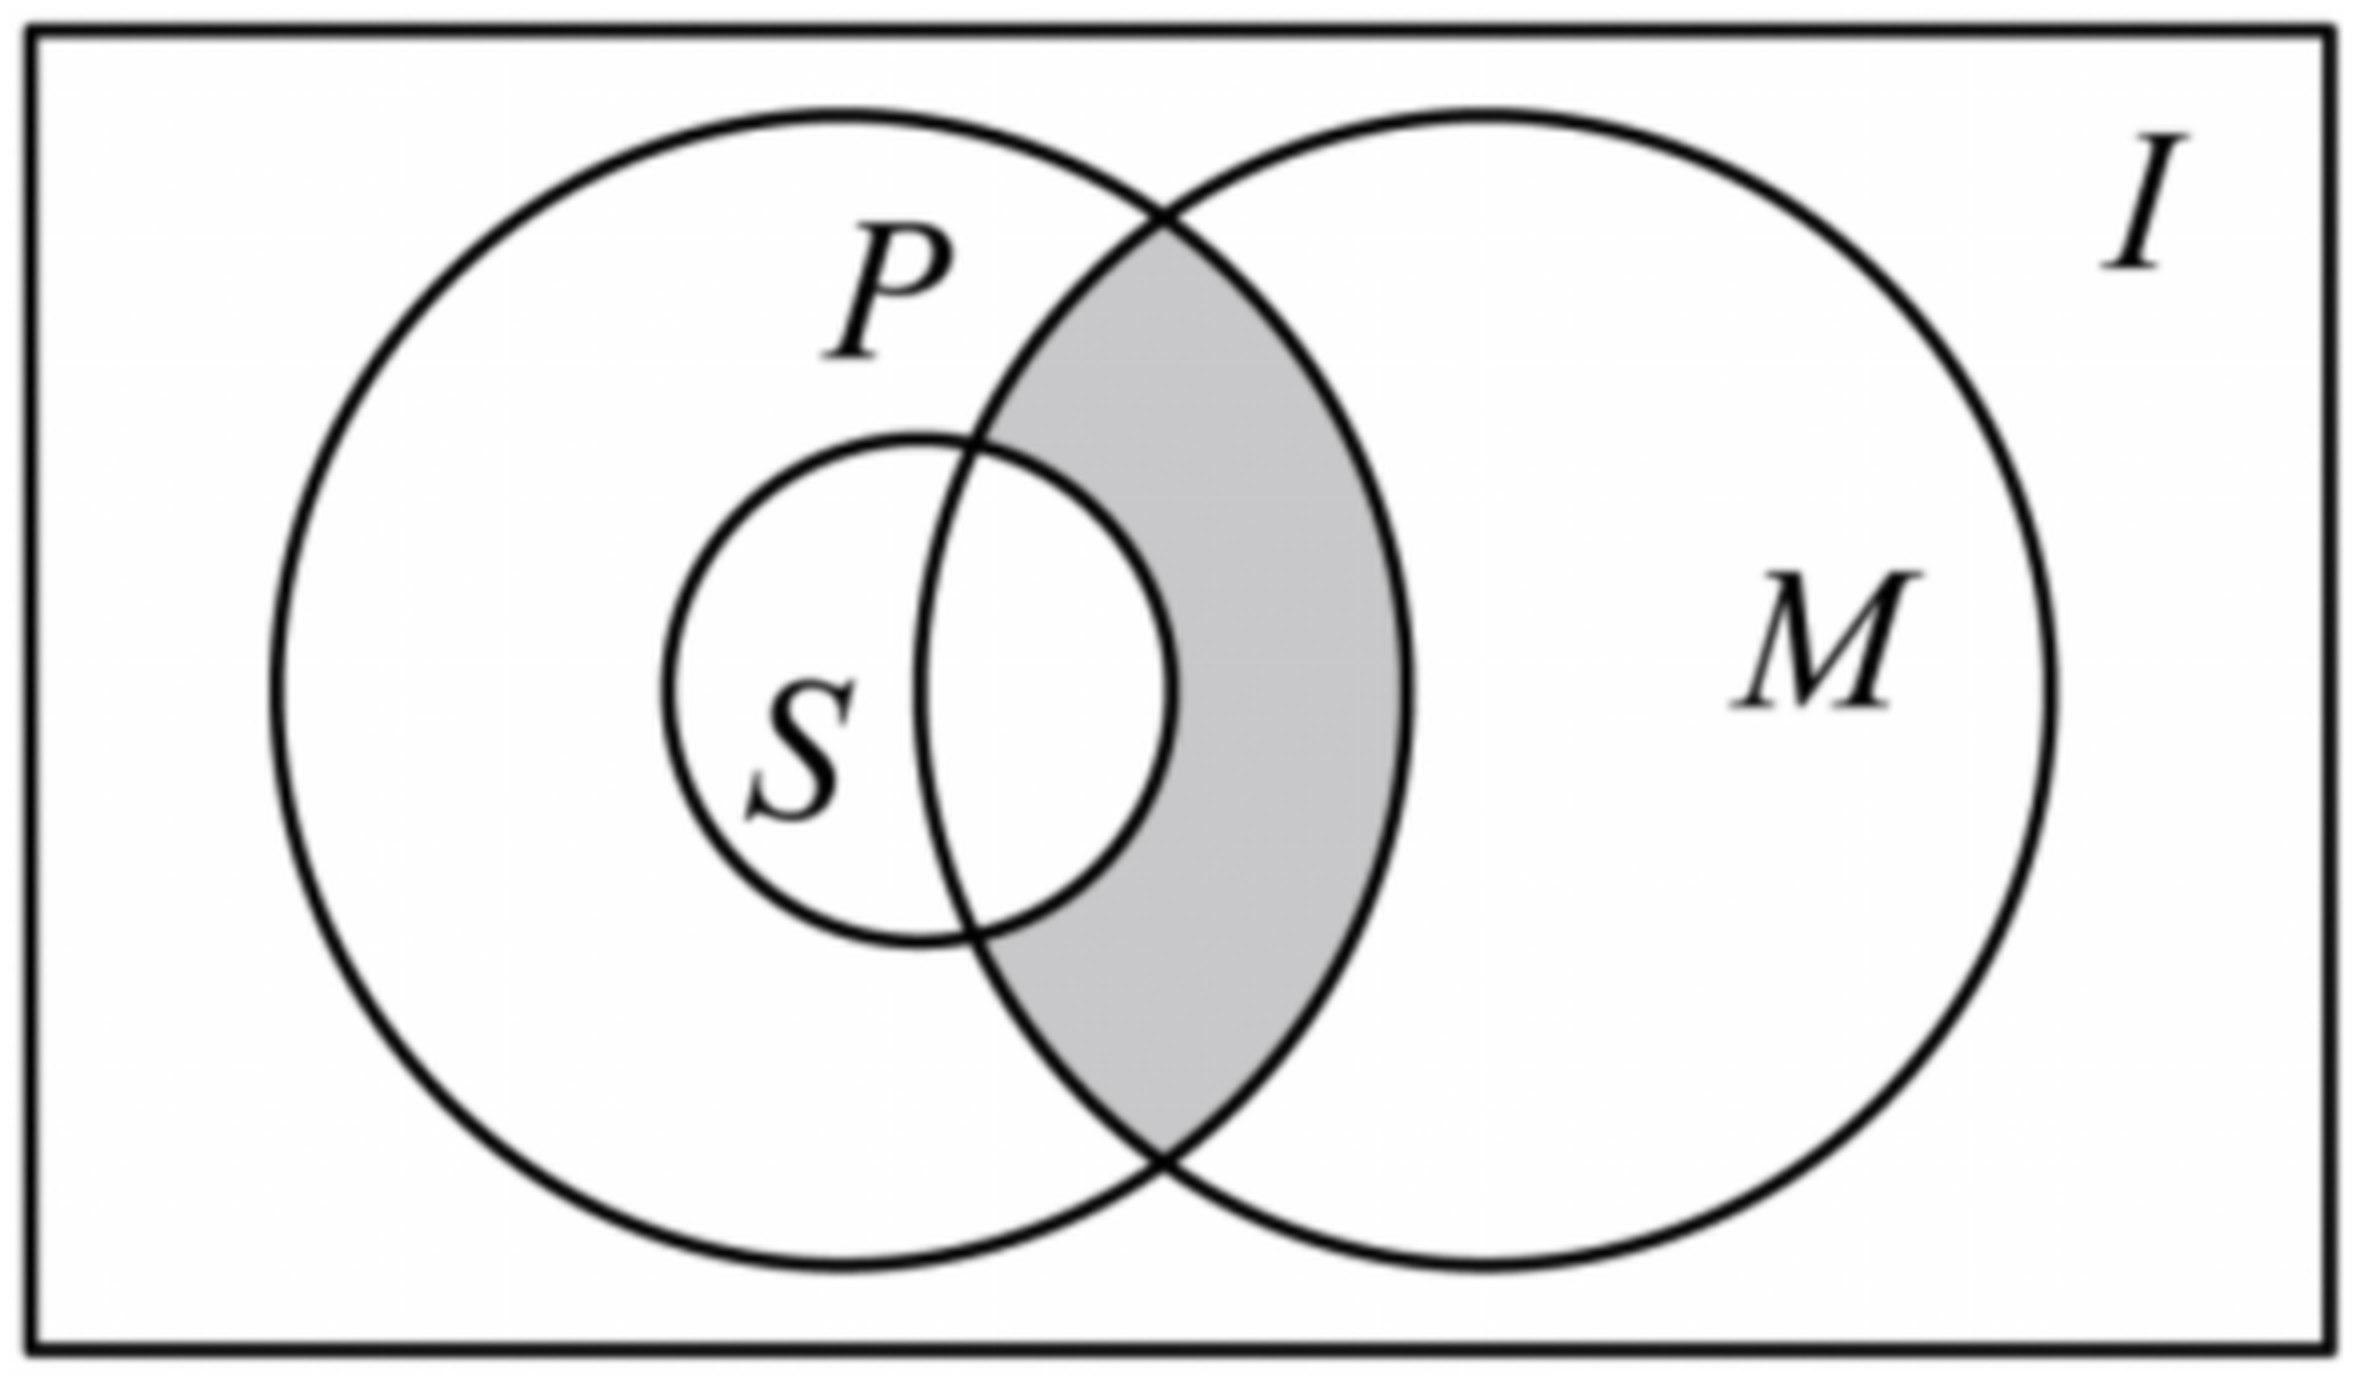
\includegraphics[width=0.46\textwidth]{figures/venn_MP_minus_S_h32.png}
\end{center}

\keepwithprev
A. $(M\cap P)\cap S$\qquad\qquad B. $(M\cap P)\cup S$

C. $(M\cap P)\cap\overline{S}$\qquad\qquad D. $(M\cap P)\cup\overline{S}$

\ans{$C$}

\ifanswer
\solbegin
\step{由 Venn 图得，集合表示 $M$、$P$ 的交集与 $S$ 的补集的交集，}
\step{即阴影部分所表示的集合是 $(M\cap P)\cap\overline{S}$. 故选 $C$.}
\solend

\fi

\item 若实数 $a$、$b$ 满足 $ab>0$，$a+2b=6$，则下列结论中错误的是\mbox{（\quad）}

\keepwithprev
A. $ab\leqslant\dfrac92$\qquad\qquad B. $a^2+4b^2\geqslant18$

C. $\dfrac1a+\dfrac2b$ 的最小值为 $\dfrac94$\qquad\qquad
D. $\dfrac{a^2}{a+1}+\dfrac{4b^2}{2b+1}$ 的最小值为 $\dfrac92$

\ans{$C$}

\ifanswer
\solbegin
\step{因为 $ab>0$，所以 $a$、$b$ 同号，又 $a+2b=6$，所以 $a$、$b$ 同正.}
\step{对于 $A$，由 $6=a+2b\geqslant2\sqrt{a\cdot2b}$ 得 $ab\leqslant\dfrac92$，故 $A$ 正确；}
\step{对于 $B$，由不等式 $\sqrt{\dfrac{m^2+n^2}2}\geqslant\dfrac{m+n}2$ 得
$\sqrt{\dfrac{a^2+(2b)^2}2}\geqslant\dfrac{a+2b}2=3$，}
\step{所以 $a^2+4b^2\geqslant18$，当且仅当 $a=2b=3$ 时取等号，故 $B$ 正确；}
\step{对于 $C$，$\dfrac1a+\dfrac2b
=\dfrac16\left(\dfrac1a+\dfrac2b\right)(a+2b)
=\dfrac16\left(5+\dfrac{2b}a+\dfrac{2a}b\right)$}
\step{$=\dfrac56+\dfrac13\left(\dfrac ba+\dfrac ab\right)
\geqslant\dfrac56+\dfrac13\times2\sqrt{\dfrac ba\cdot\dfrac ab}=\dfrac32$，}
\step{当且仅当 $\dfrac ba=\dfrac ab$，即 $a=b=2$ 时取等号，故 $C$ 错误；}
\step{对于 $D$，$\dfrac{a^2}{a+1}+\dfrac{4b^2}{2b+1}
=\dfrac{(a+1)^2-2(a+1)+1}{a+1}+\dfrac{(2b+1)^2-2(2b+1)+1}{2b+1}$}
\step{$=(a+1)-2+\dfrac1{a+1}+(2b+1)-2+\dfrac1{2b+1}
=(a+2b-2)+\dfrac1{a+1}+\dfrac1{2b+1}$}
\step{$=(6-2)+\dfrac{a+2b+2}{(a+1)(2b+1)}
=4+\dfrac8{(a+1)(2b+1)}$，}
\step{因为 $(a+1)(2b+1)\leqslant\left(\dfrac{a+1+2b+1}2\right)^2
=\left(\dfrac82\right)^2=16$，}
\step{当且仅当 $a+1=2b+1$，即 $a=2b=3$ 时取等号，}
\step{所以 $4+\dfrac8{(a+1)(2b+1)}\geqslant4+\dfrac8{16}=\dfrac92$，
故 $D$ 正确，其他几种方法同 12 题.}
\step{故选 $C$.}
\solend

\fi

% 注：本题的答案「D」原卷直接印在题干末尾的括号内，本稿按全稿惯例另提为 \ans{}。
\item 已知函数 $f(x)=x^2-2ax+a^2-1$，定义集合 $A=\{x\mid f(x)<0\}$. 若集合
$\{x\mid f(x)\in A\}=\varnothing$，则实数 $a$ 的取值范围是\mbox{（\quad）}

\keepwithprev
A. $(-3,-2)$\qquad B. $[-3,-2]$\qquad
C. $(-\infty,2)$\qquad D. $(-\infty,-2]$

\ans{$D$}

\item 非空集合 $A$ 具有如下性质：①若 $x$、$y\in A$，则 $\dfrac xy\in A$；
②若 $x$、$y\in A$，则 $x+y\in A$；

由此可知：下列判断中，错误的是\mbox{（\quad）}

\keepwithprev
A. $-1\notin A$\qquad\qquad B. $\dfrac{2025}{2026}\in A$

C. 若 $x$、$y\in A$，则 $xy\in A$\qquad\qquad
D. 若 $x$、$y\in A$，则 $x-y\in A$

\ans{$D$}

\ifanswer
\solbegin
\step{由题意得 $0\notin A$，$1\in A$，}
\step{对于 $A$，假设 $-1\in A$，则 $-1+1=0\in A$，矛盾，所以 $-1\notin A$，故 $A$ 正确；}
\step{对于 $B$，由 $1\in A$，得 $1+1=2\in A$，$2+1=3\in A$，…，$2025\in A$，$2026\in A$，}
\step{所以 $\dfrac{2025}{2026}\in A$，故 $B$ 正确；}
\step{对于 $C$，因为 $1\in A$，$x\in A$，所以 $\dfrac1x\in A$，
又因为 $y\in A$，所以 $\dfrac y{\frac1x}=xy\in A$，}
\step{故 $C$ 正确；}
\step{对于 $D$，因为 $1\in A$，$2\in A$，若 $x=1$，$y=2$，则 $x-y=-1\notin A$，故 $D$ 错误.}
\step{故选 $D$.}
\solend

\fi

\end{enumerate}

\bigsec{三、解答题}

\begin{enumerate}
\setcounter{enumi}{16}

\item 求下列关于实数 $x$ 的不等式的解集.

\begin{enumerate}[label=(\arabic*)]
\item $|2x+1|<5x-1$；
\item $\dfrac{(x-1)(x-3)(x-6)}{(x-2)(x-4)^2(x-5)}\geqslant0$.
\end{enumerate}

\ifanswer
\solbegin
\stepm{(1)}{因为不等式 $|2x+1|<5x-1$ 可化为 $-(5x-1)<2x+1<5x-1$，且 $5x-1>0$，}
\step{解得 $x>\dfrac23$，所以原不等式的解集为 $\left(\dfrac23,+\infty\right)$；}
\stepm{(2)}{不等式 $\dfrac{(x-1)(x-3)(x-6)}{(x-2)(x-4)^2(x-5)}\geqslant0$，}
\step{等价于 $(x-1)(x-3)(x-6)(x-2)(x-5)\geqslant0$，
且 $x-2\neq0$，$x-4\neq0$，$x-5\neq0$，}
\step{由“穿针引线法”，解得 $1\leqslant x<2$ 或 $3\leqslant x<4$ 或 $4<x<5$ 或 $x\geqslant6$，}
\step{所以不等式的解集为 $[1,2)\cup[3,4)\cup(4,5)\cup[6,+\infty)$.}
\solend

\fi

\ansspace[6]

\item 已知集合 $A=\left\{x\left|mx^2-mx+\dfrac{5m}2-6=0\right.\right\}\neq\varnothing$，
集合 $B=\{x\mid1<x<4$ 且 $x\in\Z\}$，$C=\{x\mid ax+3>0\}$；若 $A\cap B=A$.

\begin{enumerate}[label=(\arabic*)]
\item 求 $m$ 的取值范围.
\item 设 $m$ 的取值集合为 $D$，若 $C\cap D=\varnothing$，求 $m$ 的值及其对应 $a$ 的取值范围.
\end{enumerate}

\ans{略}

\ansspace[8]

\item 已知函数 $f(x)=x^2+(m-2)x+2m-1$.

\begin{enumerate}[label=(\arabic*)]
\item 若 $f(x)=0$ 的两根为 $x_1$、$x_2$，且 $|x_1-x_2|=2$，求实数 $m$ 的值；
\item 若函数 $y=f(x)$ 的图像在区间 $(0,1)$ 上与 $x$ 轴只有一个交点，
求实数 $m$ 的取值范围.
\end{enumerate}

\ifanswer
\solbegin
\stepm{(1)}{由题意得 $x_1+x_2=-(m-2)=2-m$，$x_1x_2=2m-1$，}
\step{由 $|x_1-x_2|=\sqrt{(x_1+x_2)^2-4x_1x_2}
=\sqrt{(2-m)^2-4(2m-1)}=2$，}
\step{化简得 $m^2-12m+4=0$，解得 $m=6\pm4\sqrt2$，故 $m=6\pm4\sqrt2$.}
\stepm{(2)}{当 $f(x)=0$ 只有一个根，且此根位于区间 $(0,1)$，}
\step{则 $\begin{cases}0<\dfrac{2-m}2<1\\[4pt]
\Delta=(m-2)^2-4(2m-1)=0\end{cases}$，
解得 $\begin{cases}0<m<2\\ m=6-2\sqrt7\text{ 或 }m=6+2\sqrt7\end{cases}$，}
\step{所以 $m=6-2\sqrt7$；}
\step{当 $f(x)=0$ 有两个根时，有一个根在区间 $(0,1)$ 内，且另一个根位于 $[0,1]$ 之外，}
\step{则 $\begin{cases}f(0)f(1)<0\\ \Delta=(m-2)^2-4(2m-1)>0\end{cases}$，
解得 $\begin{cases}\dfrac12<m<\dfrac23\\[4pt]
m<6-2\sqrt7\text{ 或 }m>6+2\sqrt7\end{cases}$，}
% 注：下一行原卷作「即 $\dfrac12<m<\dfrac32$」，按上一行方程组应为
%     $\dfrac12<m<\dfrac23$（同页最终答案也印证），照录未改，见文件头「原卷存疑」①。
\step{即 $\dfrac12<m<\dfrac32$；}
\step{当 $f(x)=0$ 有两个根位于区间 $[0,1]$ 内，且只有一个根在区间 $(0,1)$ 内，}
\step{则另一个根为 $0$ 时，得 $m=\dfrac12$，此时 $x_1+x_2=\dfrac32$，
解得另一个根 $x_2=\dfrac32>0$，故此种情况不符题意；}
\step{当 $f(x)=0$ 有两个根位于区间 $(0,1]$ 内，且只有一个根在区间 $(0,1)$ 内，}
\step{则另一个根为 $1$ 时，得 $m=\dfrac23$，此时 $x_1+x_2=\dfrac43$，
解得另一个根 $x_2=\dfrac13$，故此种情况符合题意；}
\step{综上所述，$m$ 的取值范围为
$\left(\dfrac12,\dfrac23\right]\cup\{6-2\sqrt7\}$.}
\solend

\fi

\ansspace[8]

\item 设集合 $A=\{a_1,a_2,a_3,a_4\}$，$B=\{b_1,b_2,b_3,b_4\}$，$C=\{2,3,4,6\}$，
新定义：集合 $A$ 中所有含 $k$ 个元素的子集中 $k$ 个元素之和组成的集合为“$k$ 元集和集”，
集合 $A$ 中所有含 $k$ 个元素的子集中最大元素减去剩余所有元素的和组成的集合为“$k$ 元差集”.

\begin{enumerate}[label=(\arabic*)]
\item 若 $A$ 的“$k$ 元集和集”为 $C$，求：集合 $A$.
\item 在 (1) 的条件下，若 $B$ 的“$k$ 元差集”为 $C$，求：所有满足条件的 $A\cap B$ 的真子集
个数之和.
\item 设 $b_1=a_1^2$，$b_2=a_2^2$，$b_3=a_3^2$，$b_4=a_4^2$，若 $A\cap B$ 为 $2$ 元集且
元素之和为 $10$ 且 $A$ 的“$2$ 元集和集”中最大元素不超过 $14$，求：所有满足条件的 $A$ 的
“$3$ 元差集”.
\end{enumerate}

\ifanswer
\solbegin
\stepm{(1)}{若 $A$ 的“$k$ 元集和集”为 $C$，$C=\{2,3,4,6\}$，则集合为 $\{-1,1,2,3\}$；}
\stepm{(2)}{$B$ 集合为 $\{5,3,0,-1\}$ 或 $\{9,3,1,0\}$ 或 $\{6,3,1,-1\}$，}
\step{故所有 $A\cap B$ 的真子集个数之和为 $13$；}
\stepm{(3)}{$b_1=a_1^2$，$b_2=a_2^2$，$b_3=a_3^2$，$b_4=a_4^2$，}
\step{若 $A\cap B$ 为 $2$ 元集且元素之和为 $10$，
且 $A$ 的“$2$ 元集和集”中最大元素不超过 $14$，}
% 注：下一行答案的第二个集合 $\{0,4,5,6\}$ 是 4 元集，而题问的却是「3 元差集」，
%     原卷如此，照录未改，见文件头「原卷存疑」③。
\step{则满足条件的 $A$ 的“$3$ 元差集” $\{1,3,5\}$ 或 $\{0,4,5,6\}$ 或 $\{2,4,5,8\}$.}
\solend

\fi

\ansspace[8]

\item 已知有限集 $X$、$Y$，定义集合 $X-Y=\{x\mid x\in X$ 且 $x\notin Y\}$，
$|X|$ 表示集合 $X$ 元素个数.

\begin{enumerate}[label=(\arabic*)]
\item 若 $X=\{1,2,3,4\}$，$Y=\{3,4,5\}$，写出集合 $X-Y$ 和 $Y-X$，以及
$|(X-Y)\cup(Y-X)|$ 的值；
\item 给定正整数 $n$，集合 $S=\{1,2,\cdots,n\}$，对于实数集的非空有限子集 $A$、$B$，
定义集合 $C=\{x\mid x=a+b,a\in A,b\in B\}$；

①求证：$|A-S|+|B-S|+|S-C|\geqslant1$；

②求 $|(A-S)\cup(S-A)|+|(B-S)\cup(S-B)|+|(C-S)\cup(S-C)|$ 的最小值.
\end{enumerate}

\ifanswer
\solbegin
\stepm{(1)}{由定义直接得 $X-Y=\{1,2\}$，$Y-X=\{5\}$，
$|(X-Y)\cup(Y-X)|=3$.}
% 注：下一句原卷作「显然 $|X|\geqslant0$」（按后文论证疑为 $|S|\geqslant0$），
%     照录未改，见文件头「原卷存疑」②。
\stepm{(2)}{①显然 $|X|\geqslant0$.}
\step{若 $A\cup B$ 中含有一个不在 $S$ 中的元素，则 $|A-S|+|B-S|\geqslant1$，
即 $|A-S|+|B-S|+|S-C|\geqslant1$.}
\step{若 $A\sub S$，且 $B\sub S$，则 $|A-S|=|B-S|=0$；}
\step{此时 $A$ 中最小的元素 $a\geqslant1$，$B$ 中最小的元素 $b\geqslant1$，
所以 $C$ 中最小的元素 $a+b\geqslant2$，所以 $1\notin C$.}
\step{因为 $S=\{1,2,\cdots,n\}$，所以 $|S-C|\geqslant1$，
即 $|A-S|+|B-S|+|S-C|\geqslant1$.}
\step{综上，$|A-S|+|B-S|+|S-C|\geqslant1$.}
\step{②由①得 $|A-S|+|B-S|+|S-C|\geqslant1$.}
\step{所以 $|(A-S)\cup(S-A)|+|(B-S)\cup(S-B)|+|(C-S)\cup(S-C)|$}
\step{$=|A-S|+|S-A|+|B-S|+|S-B|+|C-S|+|S-C|$}
\step{$\geqslant|S-A|+|S-B|+|C-S|+1$.}
\step{若 $A\cap S=\varnothing$，或 $B\cap S=\varnothing$，则 $|S-A|+|S-B|\geqslant n$.}
\step{若 $A\cap S\neq\varnothing$，且 $B\cap S\neq\varnothing$，
设 $A\cap S=\{a_1,a_2,\cdots,a_s\}$，$B\cap S=\{b_1,b_2,\cdots,b_t\}$，}
\step{且 $1\leqslant a_1<a_2<\cdots<a_s\leqslant n$，
$1\leqslant b_1<b_2<\cdots<b_t\leqslant n$，则 $|S-A|=n-s$，$|B-S|=n-t$.}
% 注：原卷的解析到此为止（第 10 页末），②的最小值并未给出，照录未补，
%     见文件头「原卷存疑」④。
\solend

\fi

\ansspace*[10]

\end{enumerate}

\end{document}
"
%
% 原始材料是微信公众号图文（公众号「魔都数学加油站」连载「27学年高一 32」，2026-09-25 发布，
% 原文标题「27学年高一32——2026-2027年上海市华师大二附中高一上周末作业4」），
% 正文为 10 张 PNG 页。**同一篇里各页分辨率不一致**（2560×3620 与 4762×6735 两档混排），
% 取 mmbiz.qpic.cn/<hash>/0 的原图档。原文本身就是一份**讲评版**——有的题下方印【解析】、
% 有的印【答案】，第 15 题的答案直接印在题干末尾的括号里。
% 试题文字、答案与解析均照原卷录入，未改内容。卷面的粉色斜水印属水印，未录入。
%
% ⚠ 卷首年份：本卷卷面印作「**2025-2026 年**」，与连载「27学年高一32」及公众号原文标题的
%   「2026-2027 年」**不一致**。经三人次分别把标题行裁出放大（4×—10×）独立判读，三次都读作
%   2025-2026，且校名作「华师大二附中」（无「东」字）、卷面亦无「上海市」三字。
%   按全稿「标题行照原卷」的口径，本稿照卷面排作「2025--2026 年…」——这是全稿唯一一份
%   年份不是 2026--2027 的卷子（其余 35 份均为 2026--2027）。
%
% 卷首标题：原卷印作「……年华师大二附中高一上周末作业 4」（公众号标题里的「上海市」
% 三字卷面标题行没有，本稿照卷面），年份区间按全稿惯例排 en dash，前缀照原卷保留「年」。
%
% 与原卷的排版差异（均已在 README「说明」中交代）：
%   ① 原文自**第 3 题**起（第 1、2 题未在该文中发布），故本稿题号亦自 3 起；
%   ② 原卷本就印有「一、填空题」「二、选择题」「三、解答题」三节标题，本稿照原卷分节，
%      只把标题改排成全稿统一的「大节标题」样式；
%   ③ 原卷第 6、8、9 题只印【答案】行（第 18 题的【答案】印作「略”），其余各题印【解析】，
%      第 15 题的答案直接印在题干末尾的括号内；本稿统一改为试卷版隐去、
%      答案版以 \ans{}／\ifanswer 块给出，两版彻底分离；
%   ④ 子集符号原卷两种并用：第 21(2)① 的 $A\sub S$、$B\sub S$ 带下划线，
%      第 3、10 题的 $(0,2)\subset(-\infty,3)$、$A\subset B$、$\overline{B}\subset\overline{A}$
%      作真包含，本稿分别照录为 $\sub$ 与 $\subset$；
%   ⑤ 补集符号原卷一律作上横线（$\overline{A}$、$\overline{B}$、$\overline{S}$），本稿照录；
%      空集原卷作「斜杠伸出圆外」的 $\varnothing$；
%   ⑥ 判别式记号原卷两种：第 4 题作粗体的 $\Delta$、第 11 题作细等宽的 $\triangle$，本稿照录；
%   ⑦ 数集记号原卷作斜体的 $R$、$Z$（第 4、18 题），本稿按全稿惯例统一写作 $\R$、$\Z$；
%   ⑧ 原卷填空的横线约两个字宽，本稿按全稿惯例统一排 \blankline[4.4em]；
%   ⑨ 原卷未印副标题，本稿按全稿惯例补出副标题「集合与常用逻辑用语」；
%   ⑩ 本卷只有第 13 题一图（韦恩图），原卷印在题干右侧，本稿移至题干之后；
%      图取原卷截图、4× LANCZOS 放大（figures/venn_MP_minus_S_h32.png）。
%
% 原卷存疑四处（均照抄原卷、未改，见源码中该处上方注释）：
%   ① 第 19(2)【解析】有「即 $\dfrac12<m<\dfrac32$」，按上一行的方程组应为
%      $\dfrac12<m<\dfrac23$（同页最终答案 $\left(\dfrac12,\dfrac23\right]$ 也印证）；
%   ② 第 21(2)① 首句作「显然 $|X|\geqslant0$」（按后文论证疑为 $|S|\geqslant0$）；
%   ③ 第 20(3) 的答案第二个集合 $\{0,4,5,6\}$ 是 4 元集，而题问的是「3 元差集」；
%   ④ 第 21(2)② 的解析**原卷就未写完**（第 10 页到「则 $|S-A|=n-s$，$|B-S|=n-t$」即止）。

\documentclass[a4paper,11pt]{article}
\usepackage{common}

\begin{document}

\examtitlest[3]{2025--2026 年华师大二附中高一上周末作业 4}{集合与常用逻辑用语}

\bigsec{一、填空题}

\begin{enumerate}
\setcounter{enumi}{2}

\item 设 $x$ 为实数，则“$x<3$”是“$x(x-2)<0$”的 \blankline[4.4em] 条件.

\ifanswer
\solbegin
\step{$x(x-2)<0$，解得 $0<x<2$，$(0,2)\subset(-\infty,3)$，}
\step{若 $x$ 属于“$x(x-2)<0$”，则属于“$x<3$”一定成立，即满足必要性，}
\step{若 $x$ 属于“$x<3$”，不一定满足“$x(x-2)<0$”，如 $x=-1$，即充分性不成立；}
\step{故“$x<3$”是“$x(x-2)<0$”的必要不充分条件.}
\solend

\fi

\item 若关于 $x$ 的不等式 $kx^2-kx+1>0$ 的解集为 $\R$，则实数 $k$ 的取值范围为
\blankline[4.4em].

\ifanswer
\solbegin
\step{①当 $k=0$ 时，不等式为 $1>0$ 恒成立，满足题意；}
\step{②当 $k\neq0$ 时，只要 $\begin{cases}k>0\\ \Delta=k^2-4k<0\end{cases}$，
解得 $0<k<4$；}
\step{所以不等式 $kx^2-kx+1>0$ 的解集为 $\R$，则实数 $k$ 的取值范围为 $[0,4)$.}
\solend

\fi

\item 已知 $1<a<3$，$-5<b<-2$，则 $\dfrac ab$ 的取值范围是 \blankline[4.4em].

\ifanswer
\solbegin
\step{因为 $-5<b<-2$，所以 $2<-b<5$，$\dfrac15<-\dfrac1b<\dfrac12$，又 $1<a<3$，}
\step{得 $\dfrac15<-\dfrac ab<\dfrac32$，则 $-\dfrac32<\dfrac ab<-\dfrac15$，
故 $\dfrac ab$ 的取值范围是 $\left(-\dfrac32,-\dfrac15\right)$.}
\solend

\fi

\item 关于 $x$ 的不等式 $\dfrac{ax-1}{x-a}>1$ 的解集为 $A$，且 $3\notin A$，
则实数 $a$ 的取值范围为 \blankline[4.4em].

\ans{$(-\infty,1]\cup[3,+\infty)$}

\item 若关于 $x$ 的不等式 $a\leqslant\dfrac34x^2-3x+4\leqslant b$ 的解集恰好是 $[a,b]$，
则 $b-a=$ \blankline[4.4em].

\ifanswer
\solbegin
\step{令 $f(x)=\dfrac34x^2-3x+4$，则 $f(x)$ 的对称轴为 $x=2$，}
\step{画出函数 $f(x)=\dfrac34x^2-3x+4=\dfrac34(x-2)^2+1$ 的图象，
得 $f(x)_{\min}=f(2)=1$，}
\step{由题意得 $a\leqslant1$，且 $f(a)=f(b)=b$，$a<b$，}
\step{由 $f(b)=b$ 得 $\dfrac34b^2-3b+4=b$，解得 $b=\dfrac43$（舍去）或 $b=4$，得 $b=4$，}
\step{由抛物线的对称轴为 $x=2$ 得 $a=0$，所以 $b-a=4$.}
\solend

\fi

\item 若关于 $x$ 的方程 $x^2-2kx+k+4=0$ 在 $[1,2]$ 上有解，则实数 $k$ 的取值范围为
\blankline[4.4em].

\ans{$\left[\dfrac83,5\right]$}

\item 记关于 $x$ 的方程 $x^2-2mx-2m+3=0$ 的两实根为 $x_1$、$x_2$，
则 $(x_1-2)^2+(x_2-2)^2$ 的最小值为 \blankline[4.4em].

\ans{$2$}

\item 若“$|mx^2-4x+3|\geqslant2$”的必要非充分条件是“$x\leqslant1$ 或 $x\geqslant4$”，
则实数 $m$ 的取值范围是 \blankline[4.4em].

\ifanswer
\solbegin
\step{记 $|mx^2-4x+3|\geqslant2$ 的解集为集合 $A$，
$B=\{x\mid x\leqslant1\text{ 或 }x\geqslant4\}$，}
\step{则 $\overline{A}$ 为 $|mx^2-4x+3|<2$ 的解集，$\overline{B}=\{x\mid1<x<4\}$；}
\step{因为 $B$ 是 $A$ 的必要非充分条件，所以 $A\subset B$，
得 $\overline{B}\subset\overline{A}$，}
\step{即对任意 $x\in(1,4)$，都有 $|mx^2-4x+3|<2$ 恒成立.}
\step{因为 $|mx^2-4x+3|<2$，$1<x<4$，所以 $-2<mx^2-4x+3<2$，}
\step{化简得
$-5\left(\dfrac1x\right)^2+4\left(\dfrac1x\right)
<m<-\left(\dfrac1x\right)^2+4\left(\dfrac1x\right)$；}
\step{令 $t=\dfrac1x$，$g(t)=-5t^2+4t$，$h(t)=-t^2+4t$，
且 $t\in\left(\dfrac14,1\right)$；}
\step{所以 $g(t)=-5t^2+4t=-5\left(t-\dfrac25\right)^2+\dfrac45$，
当 $t=\dfrac25$ 时，$g(t)$ 取得最大值 $\dfrac45$，}
\step{$h(t)=-t^2+4t=-(t-2)^2+4$，当 $t=\dfrac14$ 时，$h(t)$ 取得最小值，
即 $h(t)>h\left(\dfrac14\right)=\dfrac{15}{16}$；}
\step{因为对任意 $t\in\left(\dfrac14,1\right)$，$g(t)<m<h(t)$ 恒成立，
所以 $g\left(\dfrac25\right)<m\leqslant h\left(\dfrac14\right)$，}
\step{即 $\dfrac45<m\leqslant\dfrac{15}{16}$，
所以 $m$ 的取值范围是 $\left(\dfrac45,\dfrac{15}{16}\right]$.}
\solend

\fi

\item 已知关于 $x$ 的方程 $x^2+2(m-2)x+m^2-3m+3=0$ 有两个不相等的实数根 $x_1$、$x_2$，则

$\dfrac{mx_1}{x_1-1}+\dfrac{mx_2}{x_2-1}-\dfrac2{x_1+x_2-2}$ 的最大值为 \blankline[4.4em].

\ifanswer
\solbegin
\step{关于 $x$ 的方程 $x^2+2(m-2)x+m^2-3m+3=0$ 有两个不相等的实数根 $x_1$、$x_2$，}
\step{则 $\triangle=4(m-2)^2-4(m^2-3m+3)=-4m+4>0$，得 $m<1$，}
\step{且 $x_1+x_2=-2(m-2)$，$x_1x_2=m^2-3m+3$，}
\step{$\dfrac{mx_1}{x_1-1}+\dfrac{mx_2}{x_2-1}-\dfrac2{x_1+x_2-2}
=\dfrac{m[2x_1x_2-(x_1+x_2)]}{x_1x_2-(x_1+x_2)+1}+\dfrac1{m-1}$}
\step{$=\dfrac{2m(m-1)^2}{m^2-m}+\dfrac1{m-1}=2(m-1)+\dfrac1{m-1}$，}
\step{又因为 $m<1$，所以 $m-1<0$，则 $1-m>0$，}
\step{所以 $2(1-m)+\dfrac1{1-m}\geqslant2\sqrt{2(1-m)\cdot\dfrac1{1-m}}=2\sqrt2$，}
\step{当且仅当 $2(1-m)=\dfrac1{1-m}$ 时，即 $m=1-\dfrac{\sqrt2}2$ 时取等号，}
\step{所以 $2(m-1)+\dfrac1{m-1}\leqslant-2\sqrt2$，
即 $\dfrac{mx_1}{x_1-1}+\dfrac{mx_2}{x_2-1}-\dfrac2{x_1+x_2-2}$ 的最大值为 $-2\sqrt2$.}
\solend

\fi

\item 若正实数 $a$、$b$ 满足 $a+2b=ab$，则 $\dfrac4{a^2+2a}+\dfrac1{2b^2+b}$ 的最小值是
\blankline[4.4em].

\ifanswer
\solbegin
\stepm{法一}{由 $a+2b=ab$，得 $\dfrac2a+\dfrac1b=1$，}
\step{令 $x=\dfrac1a$，$y=\dfrac1b$，则 $x$、$y>0$，$2x+y=1$，$2x+1+y+2=4$，}
\step{所以 $\dfrac4{a^2+2a}+\dfrac1{2b^2+b}
=\dfrac4{\frac1{x^2}+\frac2x}+\dfrac1{\frac2{y^2}+\frac1y}
=\dfrac{4x^2}{2x+1}+\dfrac{y^2}{y+2}$（*）}
\step{$=\dfrac{(2x+1)^2-2(2x+1)+1}{2x+1}+\dfrac{(y+2)^2-4(y+2)+4}{y+2}$}
\step{$=2x-1+\dfrac1{2x+1}+y-2+\dfrac4{y+2}=\dfrac1{2x+1}+\dfrac4{y+2}-2$}
\step{$=\dfrac14\left(\dfrac1{2x+1}+\dfrac4{y+2}\right)(2x+1+y+2)-2$}
\step{$=\dfrac14\left[5+\dfrac{y+2}{2x+1}+\dfrac{4(2x+1)}{y+2}\right]-2
\geqslant\dfrac14(5+2\sqrt4)-2=\dfrac14$，}
\step{当且仅当 $\dfrac{y+2}{2x+1}=\dfrac{4(2x+1)}{y+2}$，
即 $x=\dfrac16$，$y=\dfrac23$ 时取等号，}
\step{故 $\dfrac4{a^2+2a}+\dfrac1{2b^2+b}$ 的最小值是 $\dfrac14$.}
\stepm{法二}{在法一（*）后，由权方和不等式，得
$\dfrac4{a^2+2a}+\dfrac1{2b^2+b}
=\dfrac{4x^2}{2x+1}+\dfrac{y^2}{y+2}
\geqslant\dfrac{(2x+y)^2}{2x+1+y+2}=\dfrac14$，}
\step{当且仅当……，故 $\dfrac4{a^2+2a}+\dfrac1{2b^2+b}$ 的最小值是 $\dfrac14$.}
\stepm{法三}{注意到
$\left(\dfrac{a+2}a+\dfrac{2b+1}b\right)\left(\dfrac4{a^2+2a}+\dfrac1{2b^2+b}\right)$}
\step{$\geqslant
\left(\sqrt{\dfrac{a+2}a\cdot\dfrac4{a^2+2a}}
+\sqrt{\dfrac{2b+1}b\cdot\dfrac1{2b^2+b}}\right)^2
=\left(\dfrac2a+\dfrac1b\right)^2$，}
\step{其中 $\dfrac{a+2}a+\dfrac{2b+1}b=3+\dfrac{a+2b}{ab}=4$，
$\dfrac2a+\dfrac1b=\dfrac{a+2b}{ab}=1$，}
\step{所以 $\dfrac4{a^2+2a}+\dfrac1{2b^2+b}\geqslant\dfrac14$，
当且仅当……，故 $\dfrac4{a^2+2a}+\dfrac1{2b^2+b}$ 的最小值是 $\dfrac14$.}
\solend

\fi

\end{enumerate}

\bigsec{二、选择题}

\begin{enumerate}
\setcounter{enumi}{12}

\item 如图，$I$ 为全集，$M$、$P$、$S$ 是 $I$ 的三个子集，则阴影部分所表示的集合是
\mbox{（\quad）}

\begin{center}
% 图取原卷截图、4× LANCZOS 放大（原卷把图印在题干右侧，本稿移至此处，见文件头⑩）。
% 矩形为全集 $I$，左大圆 $P$（内下方含小圆 $S$，其右侧伸入 $P$ 与 $M$ 的重叠区）、
% 右大圆 $M$；阴影是 $P$、$M$ 重叠的透镜形区域挖掉 $S$ 后剩下的部分（左缘呈弯月形）。
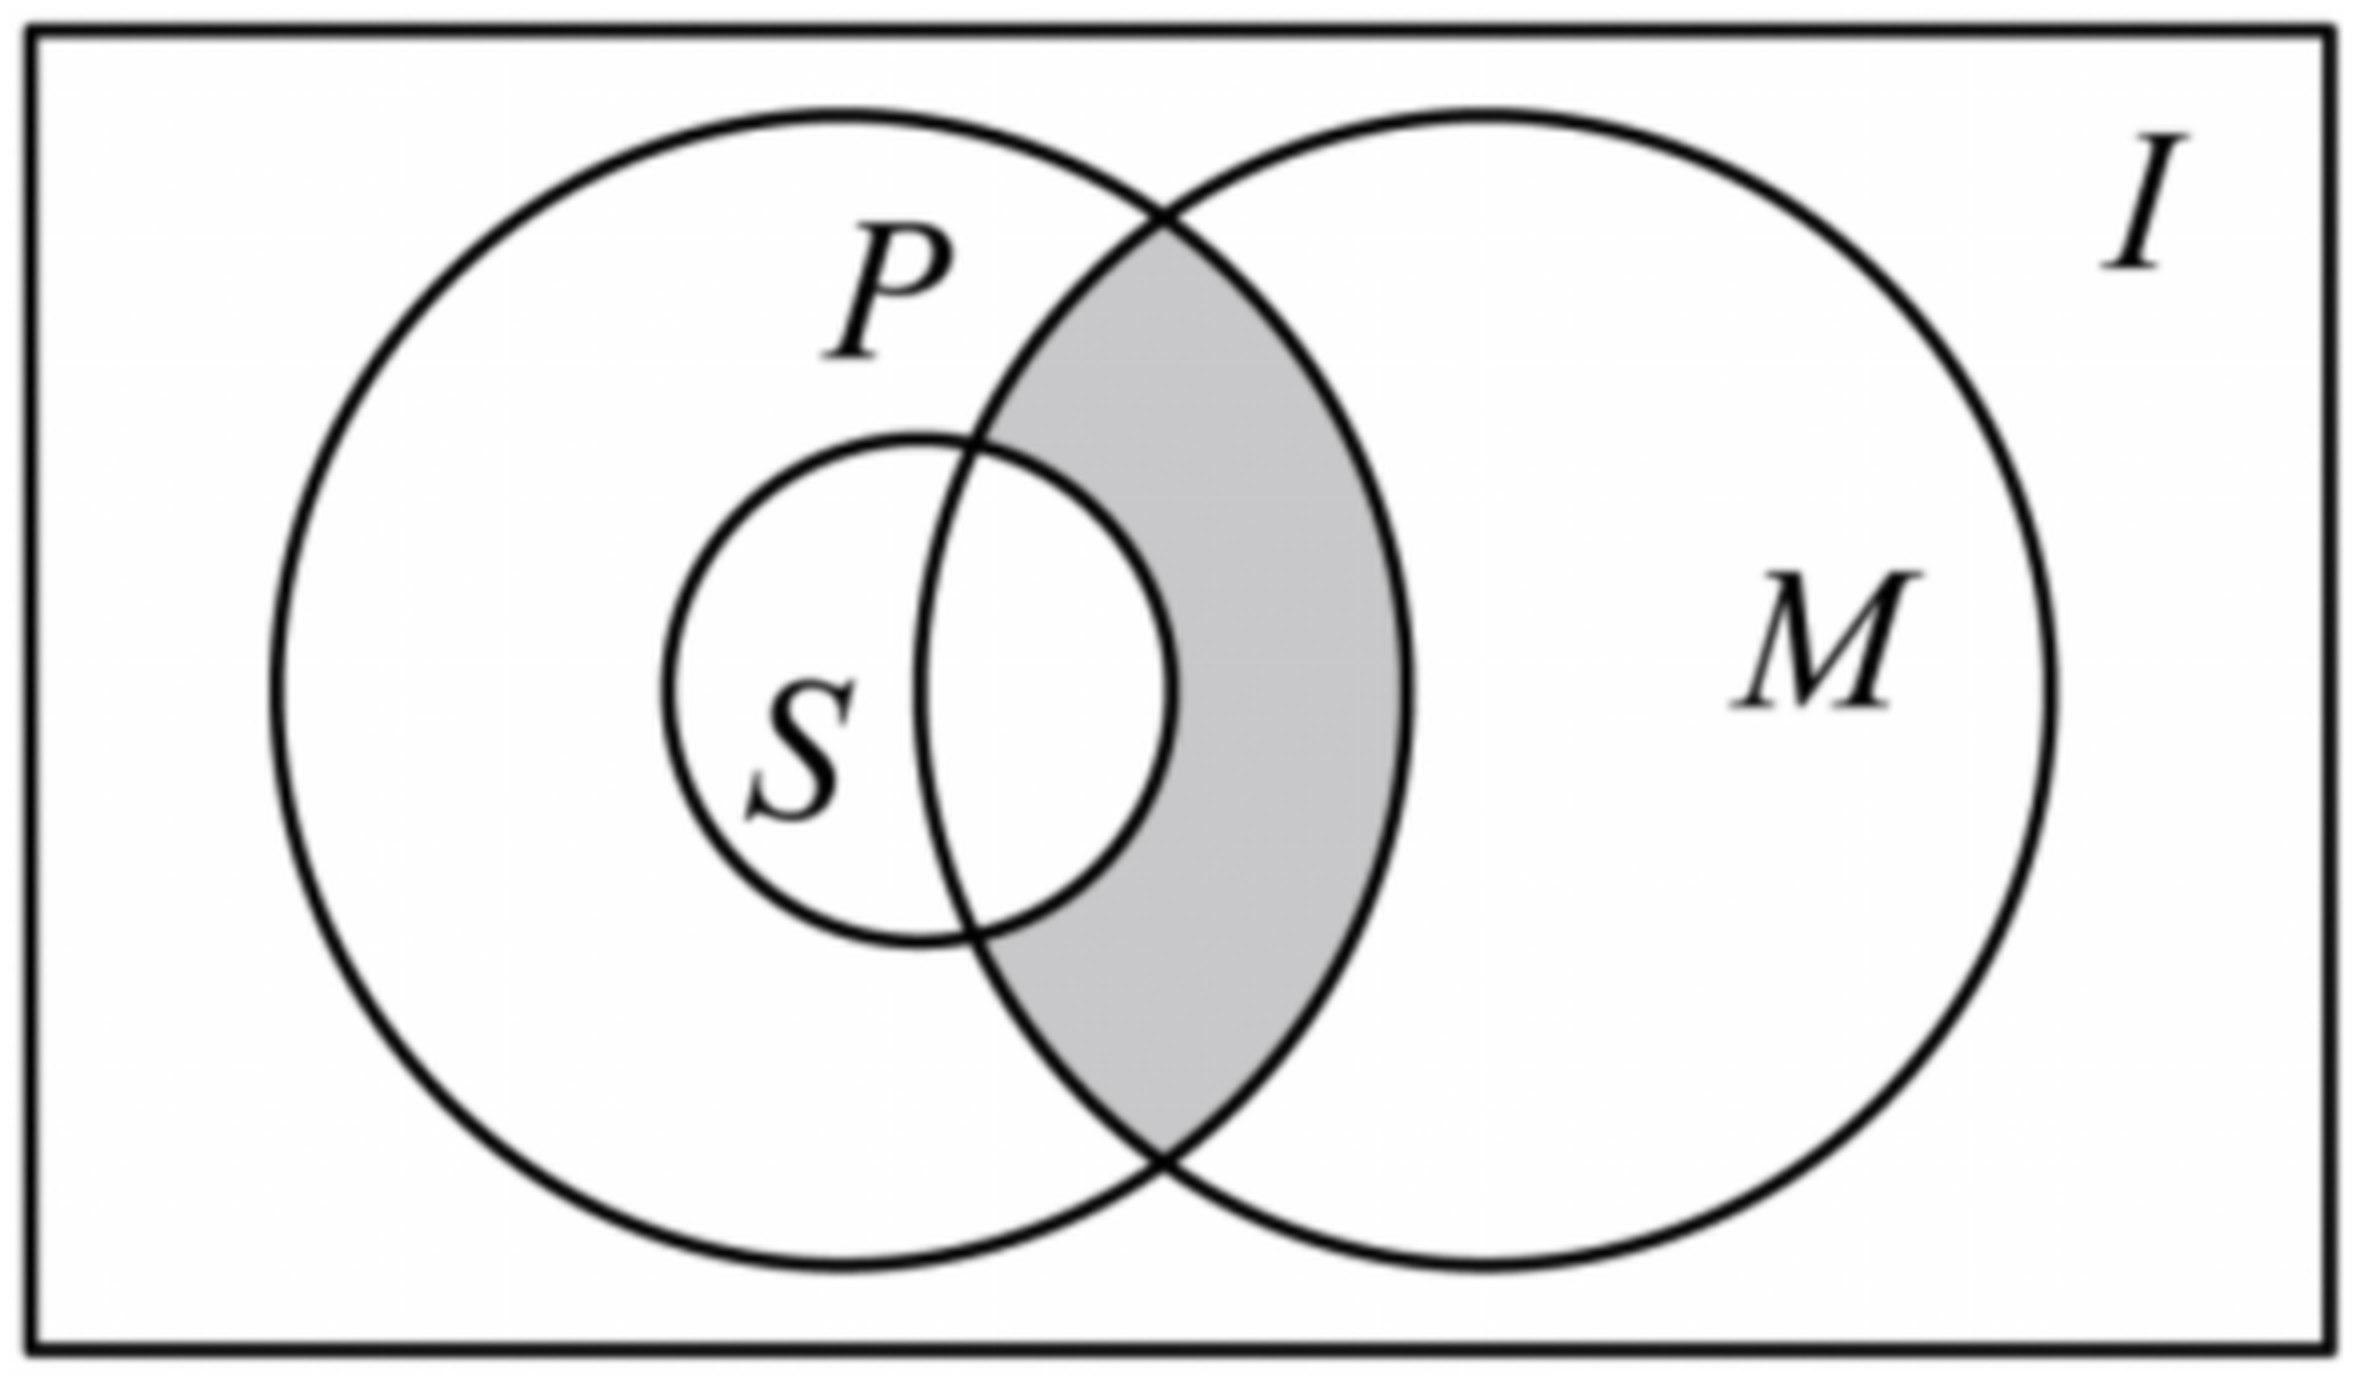
\includegraphics[width=0.46\textwidth]{figures/venn_MP_minus_S_h32.png}
\end{center}

\keepwithprev
A. $(M\cap P)\cap S$\qquad\qquad B. $(M\cap P)\cup S$

C. $(M\cap P)\cap\overline{S}$\qquad\qquad D. $(M\cap P)\cup\overline{S}$

\ans{$C$}

\ifanswer
\solbegin
\step{由 Venn 图得，集合表示 $M$、$P$ 的交集与 $S$ 的补集的交集，}
\step{即阴影部分所表示的集合是 $(M\cap P)\cap\overline{S}$. 故选 $C$.}
\solend

\fi

\item 若实数 $a$、$b$ 满足 $ab>0$，$a+2b=6$，则下列结论中错误的是\mbox{（\quad）}

\keepwithprev
A. $ab\leqslant\dfrac92$\qquad\qquad B. $a^2+4b^2\geqslant18$

C. $\dfrac1a+\dfrac2b$ 的最小值为 $\dfrac94$\qquad\qquad
D. $\dfrac{a^2}{a+1}+\dfrac{4b^2}{2b+1}$ 的最小值为 $\dfrac92$

\ans{$C$}

\ifanswer
\solbegin
\step{因为 $ab>0$，所以 $a$、$b$ 同号，又 $a+2b=6$，所以 $a$、$b$ 同正.}
\step{对于 $A$，由 $6=a+2b\geqslant2\sqrt{a\cdot2b}$ 得 $ab\leqslant\dfrac92$，故 $A$ 正确；}
\step{对于 $B$，由不等式 $\sqrt{\dfrac{m^2+n^2}2}\geqslant\dfrac{m+n}2$ 得
$\sqrt{\dfrac{a^2+(2b)^2}2}\geqslant\dfrac{a+2b}2=3$，}
\step{所以 $a^2+4b^2\geqslant18$，当且仅当 $a=2b=3$ 时取等号，故 $B$ 正确；}
\step{对于 $C$，$\dfrac1a+\dfrac2b
=\dfrac16\left(\dfrac1a+\dfrac2b\right)(a+2b)
=\dfrac16\left(5+\dfrac{2b}a+\dfrac{2a}b\right)$}
\step{$=\dfrac56+\dfrac13\left(\dfrac ba+\dfrac ab\right)
\geqslant\dfrac56+\dfrac13\times2\sqrt{\dfrac ba\cdot\dfrac ab}=\dfrac32$，}
\step{当且仅当 $\dfrac ba=\dfrac ab$，即 $a=b=2$ 时取等号，故 $C$ 错误；}
\step{对于 $D$，$\dfrac{a^2}{a+1}+\dfrac{4b^2}{2b+1}
=\dfrac{(a+1)^2-2(a+1)+1}{a+1}+\dfrac{(2b+1)^2-2(2b+1)+1}{2b+1}$}
\step{$=(a+1)-2+\dfrac1{a+1}+(2b+1)-2+\dfrac1{2b+1}
=(a+2b-2)+\dfrac1{a+1}+\dfrac1{2b+1}$}
\step{$=(6-2)+\dfrac{a+2b+2}{(a+1)(2b+1)}
=4+\dfrac8{(a+1)(2b+1)}$，}
\step{因为 $(a+1)(2b+1)\leqslant\left(\dfrac{a+1+2b+1}2\right)^2
=\left(\dfrac82\right)^2=16$，}
\step{当且仅当 $a+1=2b+1$，即 $a=2b=3$ 时取等号，}
\step{所以 $4+\dfrac8{(a+1)(2b+1)}\geqslant4+\dfrac8{16}=\dfrac92$，
故 $D$ 正确，其他几种方法同 12 题.}
\step{故选 $C$.}
\solend

\fi

% 注：本题的答案「D」原卷直接印在题干末尾的括号内，本稿按全稿惯例另提为 \ans{}。
\item 已知函数 $f(x)=x^2-2ax+a^2-1$，定义集合 $A=\{x\mid f(x)<0\}$. 若集合
$\{x\mid f(x)\in A\}=\varnothing$，则实数 $a$ 的取值范围是\mbox{（\quad）}

\keepwithprev
A. $(-3,-2)$\qquad B. $[-3,-2]$\qquad
C. $(-\infty,2)$\qquad D. $(-\infty,-2]$

\ans{$D$}

\item 非空集合 $A$ 具有如下性质：①若 $x$、$y\in A$，则 $\dfrac xy\in A$；
②若 $x$、$y\in A$，则 $x+y\in A$；

由此可知：下列判断中，错误的是\mbox{（\quad）}

\keepwithprev
A. $-1\notin A$\qquad\qquad B. $\dfrac{2025}{2026}\in A$

C. 若 $x$、$y\in A$，则 $xy\in A$\qquad\qquad
D. 若 $x$、$y\in A$，则 $x-y\in A$

\ans{$D$}

\ifanswer
\solbegin
\step{由题意得 $0\notin A$，$1\in A$，}
\step{对于 $A$，假设 $-1\in A$，则 $-1+1=0\in A$，矛盾，所以 $-1\notin A$，故 $A$ 正确；}
\step{对于 $B$，由 $1\in A$，得 $1+1=2\in A$，$2+1=3\in A$，…，$2025\in A$，$2026\in A$，}
\step{所以 $\dfrac{2025}{2026}\in A$，故 $B$ 正确；}
\step{对于 $C$，因为 $1\in A$，$x\in A$，所以 $\dfrac1x\in A$，
又因为 $y\in A$，所以 $\dfrac y{\frac1x}=xy\in A$，}
\step{故 $C$ 正确；}
\step{对于 $D$，因为 $1\in A$，$2\in A$，若 $x=1$，$y=2$，则 $x-y=-1\notin A$，故 $D$ 错误.}
\step{故选 $D$.}
\solend

\fi

\end{enumerate}

\bigsec{三、解答题}

\begin{enumerate}
\setcounter{enumi}{16}

\item 求下列关于实数 $x$ 的不等式的解集.

\begin{enumerate}[label=(\arabic*)]
\item $|2x+1|<5x-1$；
\item $\dfrac{(x-1)(x-3)(x-6)}{(x-2)(x-4)^2(x-5)}\geqslant0$.
\end{enumerate}

\ifanswer
\solbegin
\stepm{(1)}{因为不等式 $|2x+1|<5x-1$ 可化为 $-(5x-1)<2x+1<5x-1$，且 $5x-1>0$，}
\step{解得 $x>\dfrac23$，所以原不等式的解集为 $\left(\dfrac23,+\infty\right)$；}
\stepm{(2)}{不等式 $\dfrac{(x-1)(x-3)(x-6)}{(x-2)(x-4)^2(x-5)}\geqslant0$，}
\step{等价于 $(x-1)(x-3)(x-6)(x-2)(x-5)\geqslant0$，
且 $x-2\neq0$，$x-4\neq0$，$x-5\neq0$，}
\step{由“穿针引线法”，解得 $1\leqslant x<2$ 或 $3\leqslant x<4$ 或 $4<x<5$ 或 $x\geqslant6$，}
\step{所以不等式的解集为 $[1,2)\cup[3,4)\cup(4,5)\cup[6,+\infty)$.}
\solend

\fi

\ansspace[6]

\item 已知集合 $A=\left\{x\left|mx^2-mx+\dfrac{5m}2-6=0\right.\right\}\neq\varnothing$，
集合 $B=\{x\mid1<x<4$ 且 $x\in\Z\}$，$C=\{x\mid ax+3>0\}$；若 $A\cap B=A$.

\begin{enumerate}[label=(\arabic*)]
\item 求 $m$ 的取值范围.
\item 设 $m$ 的取值集合为 $D$，若 $C\cap D=\varnothing$，求 $m$ 的值及其对应 $a$ 的取值范围.
\end{enumerate}

\ans{略}

\ansspace[8]

\item 已知函数 $f(x)=x^2+(m-2)x+2m-1$.

\begin{enumerate}[label=(\arabic*)]
\item 若 $f(x)=0$ 的两根为 $x_1$、$x_2$，且 $|x_1-x_2|=2$，求实数 $m$ 的值；
\item 若函数 $y=f(x)$ 的图像在区间 $(0,1)$ 上与 $x$ 轴只有一个交点，
求实数 $m$ 的取值范围.
\end{enumerate}

\ifanswer
\solbegin
\stepm{(1)}{由题意得 $x_1+x_2=-(m-2)=2-m$，$x_1x_2=2m-1$，}
\step{由 $|x_1-x_2|=\sqrt{(x_1+x_2)^2-4x_1x_2}
=\sqrt{(2-m)^2-4(2m-1)}=2$，}
\step{化简得 $m^2-12m+4=0$，解得 $m=6\pm4\sqrt2$，故 $m=6\pm4\sqrt2$.}
\stepm{(2)}{当 $f(x)=0$ 只有一个根，且此根位于区间 $(0,1)$，}
\step{则 $\begin{cases}0<\dfrac{2-m}2<1\\[4pt]
\Delta=(m-2)^2-4(2m-1)=0\end{cases}$，
解得 $\begin{cases}0<m<2\\ m=6-2\sqrt7\text{ 或 }m=6+2\sqrt7\end{cases}$，}
\step{所以 $m=6-2\sqrt7$；}
\step{当 $f(x)=0$ 有两个根时，有一个根在区间 $(0,1)$ 内，且另一个根位于 $[0,1]$ 之外，}
\step{则 $\begin{cases}f(0)f(1)<0\\ \Delta=(m-2)^2-4(2m-1)>0\end{cases}$，
解得 $\begin{cases}\dfrac12<m<\dfrac23\\[4pt]
m<6-2\sqrt7\text{ 或 }m>6+2\sqrt7\end{cases}$，}
% 注：下一行原卷作「即 $\dfrac12<m<\dfrac32$」，按上一行方程组应为
%     $\dfrac12<m<\dfrac23$（同页最终答案也印证），照录未改，见文件头「原卷存疑」①。
\step{即 $\dfrac12<m<\dfrac32$；}
\step{当 $f(x)=0$ 有两个根位于区间 $[0,1]$ 内，且只有一个根在区间 $(0,1)$ 内，}
\step{则另一个根为 $0$ 时，得 $m=\dfrac12$，此时 $x_1+x_2=\dfrac32$，
解得另一个根 $x_2=\dfrac32>0$，故此种情况不符题意；}
\step{当 $f(x)=0$ 有两个根位于区间 $(0,1]$ 内，且只有一个根在区间 $(0,1)$ 内，}
\step{则另一个根为 $1$ 时，得 $m=\dfrac23$，此时 $x_1+x_2=\dfrac43$，
解得另一个根 $x_2=\dfrac13$，故此种情况符合题意；}
\step{综上所述，$m$ 的取值范围为
$\left(\dfrac12,\dfrac23\right]\cup\{6-2\sqrt7\}$.}
\solend

\fi

\ansspace[8]

\item 设集合 $A=\{a_1,a_2,a_3,a_4\}$，$B=\{b_1,b_2,b_3,b_4\}$，$C=\{2,3,4,6\}$，
新定义：集合 $A$ 中所有含 $k$ 个元素的子集中 $k$ 个元素之和组成的集合为“$k$ 元集和集”，
集合 $A$ 中所有含 $k$ 个元素的子集中最大元素减去剩余所有元素的和组成的集合为“$k$ 元差集”.

\begin{enumerate}[label=(\arabic*)]
\item 若 $A$ 的“$k$ 元集和集”为 $C$，求：集合 $A$.
\item 在 (1) 的条件下，若 $B$ 的“$k$ 元差集”为 $C$，求：所有满足条件的 $A\cap B$ 的真子集
个数之和.
\item 设 $b_1=a_1^2$，$b_2=a_2^2$，$b_3=a_3^2$，$b_4=a_4^2$，若 $A\cap B$ 为 $2$ 元集且
元素之和为 $10$ 且 $A$ 的“$2$ 元集和集”中最大元素不超过 $14$，求：所有满足条件的 $A$ 的
“$3$ 元差集”.
\end{enumerate}

\ifanswer
\solbegin
\stepm{(1)}{若 $A$ 的“$k$ 元集和集”为 $C$，$C=\{2,3,4,6\}$，则集合为 $\{-1,1,2,3\}$；}
\stepm{(2)}{$B$ 集合为 $\{5,3,0,-1\}$ 或 $\{9,3,1,0\}$ 或 $\{6,3,1,-1\}$，}
\step{故所有 $A\cap B$ 的真子集个数之和为 $13$；}
\stepm{(3)}{$b_1=a_1^2$，$b_2=a_2^2$，$b_3=a_3^2$，$b_4=a_4^2$，}
\step{若 $A\cap B$ 为 $2$ 元集且元素之和为 $10$，
且 $A$ 的“$2$ 元集和集”中最大元素不超过 $14$，}
% 注：下一行答案的第二个集合 $\{0,4,5,6\}$ 是 4 元集，而题问的却是「3 元差集」，
%     原卷如此，照录未改，见文件头「原卷存疑」③。
\step{则满足条件的 $A$ 的“$3$ 元差集” $\{1,3,5\}$ 或 $\{0,4,5,6\}$ 或 $\{2,4,5,8\}$.}
\solend

\fi

\ansspace[8]

\item 已知有限集 $X$、$Y$，定义集合 $X-Y=\{x\mid x\in X$ 且 $x\notin Y\}$，
$|X|$ 表示集合 $X$ 元素个数.

\begin{enumerate}[label=(\arabic*)]
\item 若 $X=\{1,2,3,4\}$，$Y=\{3,4,5\}$，写出集合 $X-Y$ 和 $Y-X$，以及
$|(X-Y)\cup(Y-X)|$ 的值；
\item 给定正整数 $n$，集合 $S=\{1,2,\cdots,n\}$，对于实数集的非空有限子集 $A$、$B$，
定义集合 $C=\{x\mid x=a+b,a\in A,b\in B\}$；

①求证：$|A-S|+|B-S|+|S-C|\geqslant1$；

②求 $|(A-S)\cup(S-A)|+|(B-S)\cup(S-B)|+|(C-S)\cup(S-C)|$ 的最小值.
\end{enumerate}

\ifanswer
\solbegin
\stepm{(1)}{由定义直接得 $X-Y=\{1,2\}$，$Y-X=\{5\}$，
$|(X-Y)\cup(Y-X)|=3$.}
% 注：下一句原卷作「显然 $|X|\geqslant0$」（按后文论证疑为 $|S|\geqslant0$），
%     照录未改，见文件头「原卷存疑」②。
\stepm{(2)}{①显然 $|X|\geqslant0$.}
\step{若 $A\cup B$ 中含有一个不在 $S$ 中的元素，则 $|A-S|+|B-S|\geqslant1$，
即 $|A-S|+|B-S|+|S-C|\geqslant1$.}
\step{若 $A\sub S$，且 $B\sub S$，则 $|A-S|=|B-S|=0$；}
\step{此时 $A$ 中最小的元素 $a\geqslant1$，$B$ 中最小的元素 $b\geqslant1$，
所以 $C$ 中最小的元素 $a+b\geqslant2$，所以 $1\notin C$.}
\step{因为 $S=\{1,2,\cdots,n\}$，所以 $|S-C|\geqslant1$，
即 $|A-S|+|B-S|+|S-C|\geqslant1$.}
\step{综上，$|A-S|+|B-S|+|S-C|\geqslant1$.}
\step{②由①得 $|A-S|+|B-S|+|S-C|\geqslant1$.}
\step{所以 $|(A-S)\cup(S-A)|+|(B-S)\cup(S-B)|+|(C-S)\cup(S-C)|$}
\step{$=|A-S|+|S-A|+|B-S|+|S-B|+|C-S|+|S-C|$}
\step{$\geqslant|S-A|+|S-B|+|C-S|+1$.}
\step{若 $A\cap S=\varnothing$，或 $B\cap S=\varnothing$，则 $|S-A|+|S-B|\geqslant n$.}
\step{若 $A\cap S\neq\varnothing$，且 $B\cap S\neq\varnothing$，
设 $A\cap S=\{a_1,a_2,\cdots,a_s\}$，$B\cap S=\{b_1,b_2,\cdots,b_t\}$，}
\step{且 $1\leqslant a_1<a_2<\cdots<a_s\leqslant n$，
$1\leqslant b_1<b_2<\cdots<b_t\leqslant n$，则 $|S-A|=n-s$，$|B-S|=n-t$.}
% 注：原卷的解析到此为止（第 10 页末），②的最小值并未给出，照录未补，
%     见文件头「原卷存疑」④。
\solend

\fi

\ansspace*[10]

\end{enumerate}

\end{document}
"
% 紧凑版：xelatex "\def\iscompact{1}% 高一32_华师大二附中_周末作业4.tex
%   —— 高一上数学「2026-2027 年华师大二附中高一上周末作业 4」（试卷版/答案版）
% 试卷版：xelatex 高一32_华师大二附中_周末作业4.tex
% 答案版：xelatex "\def\isanswer{1}% 高一32_华师大二附中_周末作业4.tex
%   —— 高一上数学「2026-2027 年华师大二附中高一上周末作业 4」（试卷版/答案版）
% 试卷版：xelatex 高一32_华师大二附中_周末作业4.tex
% 答案版：xelatex "\def\isanswer{1}% 高一32_华师大二附中_周末作业4.tex
%   —— 高一上数学「2026-2027 年华师大二附中高一上周末作业 4」（试卷版/答案版）
% 试卷版：xelatex 高一32_华师大二附中_周末作业4.tex
% 答案版：xelatex "\def\isanswer{1}\input{高一32_华师大二附中_周末作业4.tex}"
% 紧凑版：xelatex "\def\iscompact{1}\input{高一32_华师大二附中_周末作业4.tex}"
%
% 原始材料是微信公众号图文（公众号「魔都数学加油站」连载「27学年高一 32」，2026-09-25 发布，
% 原文标题「27学年高一32——2026-2027年上海市华师大二附中高一上周末作业4」），
% 正文为 10 张 PNG 页。**同一篇里各页分辨率不一致**（2560×3620 与 4762×6735 两档混排），
% 取 mmbiz.qpic.cn/<hash>/0 的原图档。原文本身就是一份**讲评版**——有的题下方印【解析】、
% 有的印【答案】，第 15 题的答案直接印在题干末尾的括号里。
% 试题文字、答案与解析均照原卷录入，未改内容。卷面的粉色斜水印属水印，未录入。
%
% ⚠ 卷首年份：本卷卷面印作「**2025-2026 年**」，与连载「27学年高一32」及公众号原文标题的
%   「2026-2027 年」**不一致**。经三人次分别把标题行裁出放大（4×—10×）独立判读，三次都读作
%   2025-2026，且校名作「华师大二附中」（无「东」字）、卷面亦无「上海市」三字。
%   按全稿「标题行照原卷」的口径，本稿照卷面排作「2025--2026 年…」——这是全稿唯一一份
%   年份不是 2026--2027 的卷子（其余 35 份均为 2026--2027）。
%
% 卷首标题：原卷印作「……年华师大二附中高一上周末作业 4」（公众号标题里的「上海市」
% 三字卷面标题行没有，本稿照卷面），年份区间按全稿惯例排 en dash，前缀照原卷保留「年」。
%
% 与原卷的排版差异（均已在 README「说明」中交代）：
%   ① 原文自**第 3 题**起（第 1、2 题未在该文中发布），故本稿题号亦自 3 起；
%   ② 原卷本就印有「一、填空题」「二、选择题」「三、解答题」三节标题，本稿照原卷分节，
%      只把标题改排成全稿统一的「大节标题」样式；
%   ③ 原卷第 6、8、9 题只印【答案】行（第 18 题的【答案】印作「略”），其余各题印【解析】，
%      第 15 题的答案直接印在题干末尾的括号内；本稿统一改为试卷版隐去、
%      答案版以 \ans{}／\ifanswer 块给出，两版彻底分离；
%   ④ 子集符号原卷两种并用：第 21(2)① 的 $A\sub S$、$B\sub S$ 带下划线，
%      第 3、10 题的 $(0,2)\subset(-\infty,3)$、$A\subset B$、$\overline{B}\subset\overline{A}$
%      作真包含，本稿分别照录为 $\sub$ 与 $\subset$；
%   ⑤ 补集符号原卷一律作上横线（$\overline{A}$、$\overline{B}$、$\overline{S}$），本稿照录；
%      空集原卷作「斜杠伸出圆外」的 $\varnothing$；
%   ⑥ 判别式记号原卷两种：第 4 题作粗体的 $\Delta$、第 11 题作细等宽的 $\triangle$，本稿照录；
%   ⑦ 数集记号原卷作斜体的 $R$、$Z$（第 4、18 题），本稿按全稿惯例统一写作 $\R$、$\Z$；
%   ⑧ 原卷填空的横线约两个字宽，本稿按全稿惯例统一排 \blankline[4.4em]；
%   ⑨ 原卷未印副标题，本稿按全稿惯例补出副标题「集合与常用逻辑用语」；
%   ⑩ 本卷只有第 13 题一图（韦恩图），原卷印在题干右侧，本稿移至题干之后；
%      图取原卷截图、4× LANCZOS 放大（figures/venn_MP_minus_S_h32.png）。
%
% 原卷存疑四处（均照抄原卷、未改，见源码中该处上方注释）：
%   ① 第 19(2)【解析】有「即 $\dfrac12<m<\dfrac32$」，按上一行的方程组应为
%      $\dfrac12<m<\dfrac23$（同页最终答案 $\left(\dfrac12,\dfrac23\right]$ 也印证）；
%   ② 第 21(2)① 首句作「显然 $|X|\geqslant0$」（按后文论证疑为 $|S|\geqslant0$）；
%   ③ 第 20(3) 的答案第二个集合 $\{0,4,5,6\}$ 是 4 元集，而题问的是「3 元差集」；
%   ④ 第 21(2)② 的解析**原卷就未写完**（第 10 页到「则 $|S-A|=n-s$，$|B-S|=n-t$」即止）。

\documentclass[a4paper,11pt]{article}
\usepackage{common}

\begin{document}

\examtitlest[3]{2025--2026 年华师大二附中高一上周末作业 4}{集合与常用逻辑用语}

\bigsec{一、填空题}

\begin{enumerate}
\setcounter{enumi}{2}

\item 设 $x$ 为实数，则“$x<3$”是“$x(x-2)<0$”的 \blankline[4.4em] 条件.

\ifanswer
\solbegin
\step{$x(x-2)<0$，解得 $0<x<2$，$(0,2)\subset(-\infty,3)$，}
\step{若 $x$ 属于“$x(x-2)<0$”，则属于“$x<3$”一定成立，即满足必要性，}
\step{若 $x$ 属于“$x<3$”，不一定满足“$x(x-2)<0$”，如 $x=-1$，即充分性不成立；}
\step{故“$x<3$”是“$x(x-2)<0$”的必要不充分条件.}
\solend

\fi

\item 若关于 $x$ 的不等式 $kx^2-kx+1>0$ 的解集为 $\R$，则实数 $k$ 的取值范围为
\blankline[4.4em].

\ifanswer
\solbegin
\step{①当 $k=0$ 时，不等式为 $1>0$ 恒成立，满足题意；}
\step{②当 $k\neq0$ 时，只要 $\begin{cases}k>0\\ \Delta=k^2-4k<0\end{cases}$，
解得 $0<k<4$；}
\step{所以不等式 $kx^2-kx+1>0$ 的解集为 $\R$，则实数 $k$ 的取值范围为 $[0,4)$.}
\solend

\fi

\item 已知 $1<a<3$，$-5<b<-2$，则 $\dfrac ab$ 的取值范围是 \blankline[4.4em].

\ifanswer
\solbegin
\step{因为 $-5<b<-2$，所以 $2<-b<5$，$\dfrac15<-\dfrac1b<\dfrac12$，又 $1<a<3$，}
\step{得 $\dfrac15<-\dfrac ab<\dfrac32$，则 $-\dfrac32<\dfrac ab<-\dfrac15$，
故 $\dfrac ab$ 的取值范围是 $\left(-\dfrac32,-\dfrac15\right)$.}
\solend

\fi

\item 关于 $x$ 的不等式 $\dfrac{ax-1}{x-a}>1$ 的解集为 $A$，且 $3\notin A$，
则实数 $a$ 的取值范围为 \blankline[4.4em].

\ans{$(-\infty,1]\cup[3,+\infty)$}

\item 若关于 $x$ 的不等式 $a\leqslant\dfrac34x^2-3x+4\leqslant b$ 的解集恰好是 $[a,b]$，
则 $b-a=$ \blankline[4.4em].

\ifanswer
\solbegin
\step{令 $f(x)=\dfrac34x^2-3x+4$，则 $f(x)$ 的对称轴为 $x=2$，}
\step{画出函数 $f(x)=\dfrac34x^2-3x+4=\dfrac34(x-2)^2+1$ 的图象，
得 $f(x)_{\min}=f(2)=1$，}
\step{由题意得 $a\leqslant1$，且 $f(a)=f(b)=b$，$a<b$，}
\step{由 $f(b)=b$ 得 $\dfrac34b^2-3b+4=b$，解得 $b=\dfrac43$（舍去）或 $b=4$，得 $b=4$，}
\step{由抛物线的对称轴为 $x=2$ 得 $a=0$，所以 $b-a=4$.}
\solend

\fi

\item 若关于 $x$ 的方程 $x^2-2kx+k+4=0$ 在 $[1,2]$ 上有解，则实数 $k$ 的取值范围为
\blankline[4.4em].

\ans{$\left[\dfrac83,5\right]$}

\item 记关于 $x$ 的方程 $x^2-2mx-2m+3=0$ 的两实根为 $x_1$、$x_2$，
则 $(x_1-2)^2+(x_2-2)^2$ 的最小值为 \blankline[4.4em].

\ans{$2$}

\item 若“$|mx^2-4x+3|\geqslant2$”的必要非充分条件是“$x\leqslant1$ 或 $x\geqslant4$”，
则实数 $m$ 的取值范围是 \blankline[4.4em].

\ifanswer
\solbegin
\step{记 $|mx^2-4x+3|\geqslant2$ 的解集为集合 $A$，
$B=\{x\mid x\leqslant1\text{ 或 }x\geqslant4\}$，}
\step{则 $\overline{A}$ 为 $|mx^2-4x+3|<2$ 的解集，$\overline{B}=\{x\mid1<x<4\}$；}
\step{因为 $B$ 是 $A$ 的必要非充分条件，所以 $A\subset B$，
得 $\overline{B}\subset\overline{A}$，}
\step{即对任意 $x\in(1,4)$，都有 $|mx^2-4x+3|<2$ 恒成立.}
\step{因为 $|mx^2-4x+3|<2$，$1<x<4$，所以 $-2<mx^2-4x+3<2$，}
\step{化简得
$-5\left(\dfrac1x\right)^2+4\left(\dfrac1x\right)
<m<-\left(\dfrac1x\right)^2+4\left(\dfrac1x\right)$；}
\step{令 $t=\dfrac1x$，$g(t)=-5t^2+4t$，$h(t)=-t^2+4t$，
且 $t\in\left(\dfrac14,1\right)$；}
\step{所以 $g(t)=-5t^2+4t=-5\left(t-\dfrac25\right)^2+\dfrac45$，
当 $t=\dfrac25$ 时，$g(t)$ 取得最大值 $\dfrac45$，}
\step{$h(t)=-t^2+4t=-(t-2)^2+4$，当 $t=\dfrac14$ 时，$h(t)$ 取得最小值，
即 $h(t)>h\left(\dfrac14\right)=\dfrac{15}{16}$；}
\step{因为对任意 $t\in\left(\dfrac14,1\right)$，$g(t)<m<h(t)$ 恒成立，
所以 $g\left(\dfrac25\right)<m\leqslant h\left(\dfrac14\right)$，}
\step{即 $\dfrac45<m\leqslant\dfrac{15}{16}$，
所以 $m$ 的取值范围是 $\left(\dfrac45,\dfrac{15}{16}\right]$.}
\solend

\fi

\item 已知关于 $x$ 的方程 $x^2+2(m-2)x+m^2-3m+3=0$ 有两个不相等的实数根 $x_1$、$x_2$，则

$\dfrac{mx_1}{x_1-1}+\dfrac{mx_2}{x_2-1}-\dfrac2{x_1+x_2-2}$ 的最大值为 \blankline[4.4em].

\ifanswer
\solbegin
\step{关于 $x$ 的方程 $x^2+2(m-2)x+m^2-3m+3=0$ 有两个不相等的实数根 $x_1$、$x_2$，}
\step{则 $\triangle=4(m-2)^2-4(m^2-3m+3)=-4m+4>0$，得 $m<1$，}
\step{且 $x_1+x_2=-2(m-2)$，$x_1x_2=m^2-3m+3$，}
\step{$\dfrac{mx_1}{x_1-1}+\dfrac{mx_2}{x_2-1}-\dfrac2{x_1+x_2-2}
=\dfrac{m[2x_1x_2-(x_1+x_2)]}{x_1x_2-(x_1+x_2)+1}+\dfrac1{m-1}$}
\step{$=\dfrac{2m(m-1)^2}{m^2-m}+\dfrac1{m-1}=2(m-1)+\dfrac1{m-1}$，}
\step{又因为 $m<1$，所以 $m-1<0$，则 $1-m>0$，}
\step{所以 $2(1-m)+\dfrac1{1-m}\geqslant2\sqrt{2(1-m)\cdot\dfrac1{1-m}}=2\sqrt2$，}
\step{当且仅当 $2(1-m)=\dfrac1{1-m}$ 时，即 $m=1-\dfrac{\sqrt2}2$ 时取等号，}
\step{所以 $2(m-1)+\dfrac1{m-1}\leqslant-2\sqrt2$，
即 $\dfrac{mx_1}{x_1-1}+\dfrac{mx_2}{x_2-1}-\dfrac2{x_1+x_2-2}$ 的最大值为 $-2\sqrt2$.}
\solend

\fi

\item 若正实数 $a$、$b$ 满足 $a+2b=ab$，则 $\dfrac4{a^2+2a}+\dfrac1{2b^2+b}$ 的最小值是
\blankline[4.4em].

\ifanswer
\solbegin
\stepm{法一}{由 $a+2b=ab$，得 $\dfrac2a+\dfrac1b=1$，}
\step{令 $x=\dfrac1a$，$y=\dfrac1b$，则 $x$、$y>0$，$2x+y=1$，$2x+1+y+2=4$，}
\step{所以 $\dfrac4{a^2+2a}+\dfrac1{2b^2+b}
=\dfrac4{\frac1{x^2}+\frac2x}+\dfrac1{\frac2{y^2}+\frac1y}
=\dfrac{4x^2}{2x+1}+\dfrac{y^2}{y+2}$（*）}
\step{$=\dfrac{(2x+1)^2-2(2x+1)+1}{2x+1}+\dfrac{(y+2)^2-4(y+2)+4}{y+2}$}
\step{$=2x-1+\dfrac1{2x+1}+y-2+\dfrac4{y+2}=\dfrac1{2x+1}+\dfrac4{y+2}-2$}
\step{$=\dfrac14\left(\dfrac1{2x+1}+\dfrac4{y+2}\right)(2x+1+y+2)-2$}
\step{$=\dfrac14\left[5+\dfrac{y+2}{2x+1}+\dfrac{4(2x+1)}{y+2}\right]-2
\geqslant\dfrac14(5+2\sqrt4)-2=\dfrac14$，}
\step{当且仅当 $\dfrac{y+2}{2x+1}=\dfrac{4(2x+1)}{y+2}$，
即 $x=\dfrac16$，$y=\dfrac23$ 时取等号，}
\step{故 $\dfrac4{a^2+2a}+\dfrac1{2b^2+b}$ 的最小值是 $\dfrac14$.}
\stepm{法二}{在法一（*）后，由权方和不等式，得
$\dfrac4{a^2+2a}+\dfrac1{2b^2+b}
=\dfrac{4x^2}{2x+1}+\dfrac{y^2}{y+2}
\geqslant\dfrac{(2x+y)^2}{2x+1+y+2}=\dfrac14$，}
\step{当且仅当……，故 $\dfrac4{a^2+2a}+\dfrac1{2b^2+b}$ 的最小值是 $\dfrac14$.}
\stepm{法三}{注意到
$\left(\dfrac{a+2}a+\dfrac{2b+1}b\right)\left(\dfrac4{a^2+2a}+\dfrac1{2b^2+b}\right)$}
\step{$\geqslant
\left(\sqrt{\dfrac{a+2}a\cdot\dfrac4{a^2+2a}}
+\sqrt{\dfrac{2b+1}b\cdot\dfrac1{2b^2+b}}\right)^2
=\left(\dfrac2a+\dfrac1b\right)^2$，}
\step{其中 $\dfrac{a+2}a+\dfrac{2b+1}b=3+\dfrac{a+2b}{ab}=4$，
$\dfrac2a+\dfrac1b=\dfrac{a+2b}{ab}=1$，}
\step{所以 $\dfrac4{a^2+2a}+\dfrac1{2b^2+b}\geqslant\dfrac14$，
当且仅当……，故 $\dfrac4{a^2+2a}+\dfrac1{2b^2+b}$ 的最小值是 $\dfrac14$.}
\solend

\fi

\end{enumerate}

\bigsec{二、选择题}

\begin{enumerate}
\setcounter{enumi}{12}

\item 如图，$I$ 为全集，$M$、$P$、$S$ 是 $I$ 的三个子集，则阴影部分所表示的集合是
\mbox{（\quad）}

\begin{center}
% 图取原卷截图、4× LANCZOS 放大（原卷把图印在题干右侧，本稿移至此处，见文件头⑩）。
% 矩形为全集 $I$，左大圆 $P$（内下方含小圆 $S$，其右侧伸入 $P$ 与 $M$ 的重叠区）、
% 右大圆 $M$；阴影是 $P$、$M$ 重叠的透镜形区域挖掉 $S$ 后剩下的部分（左缘呈弯月形）。
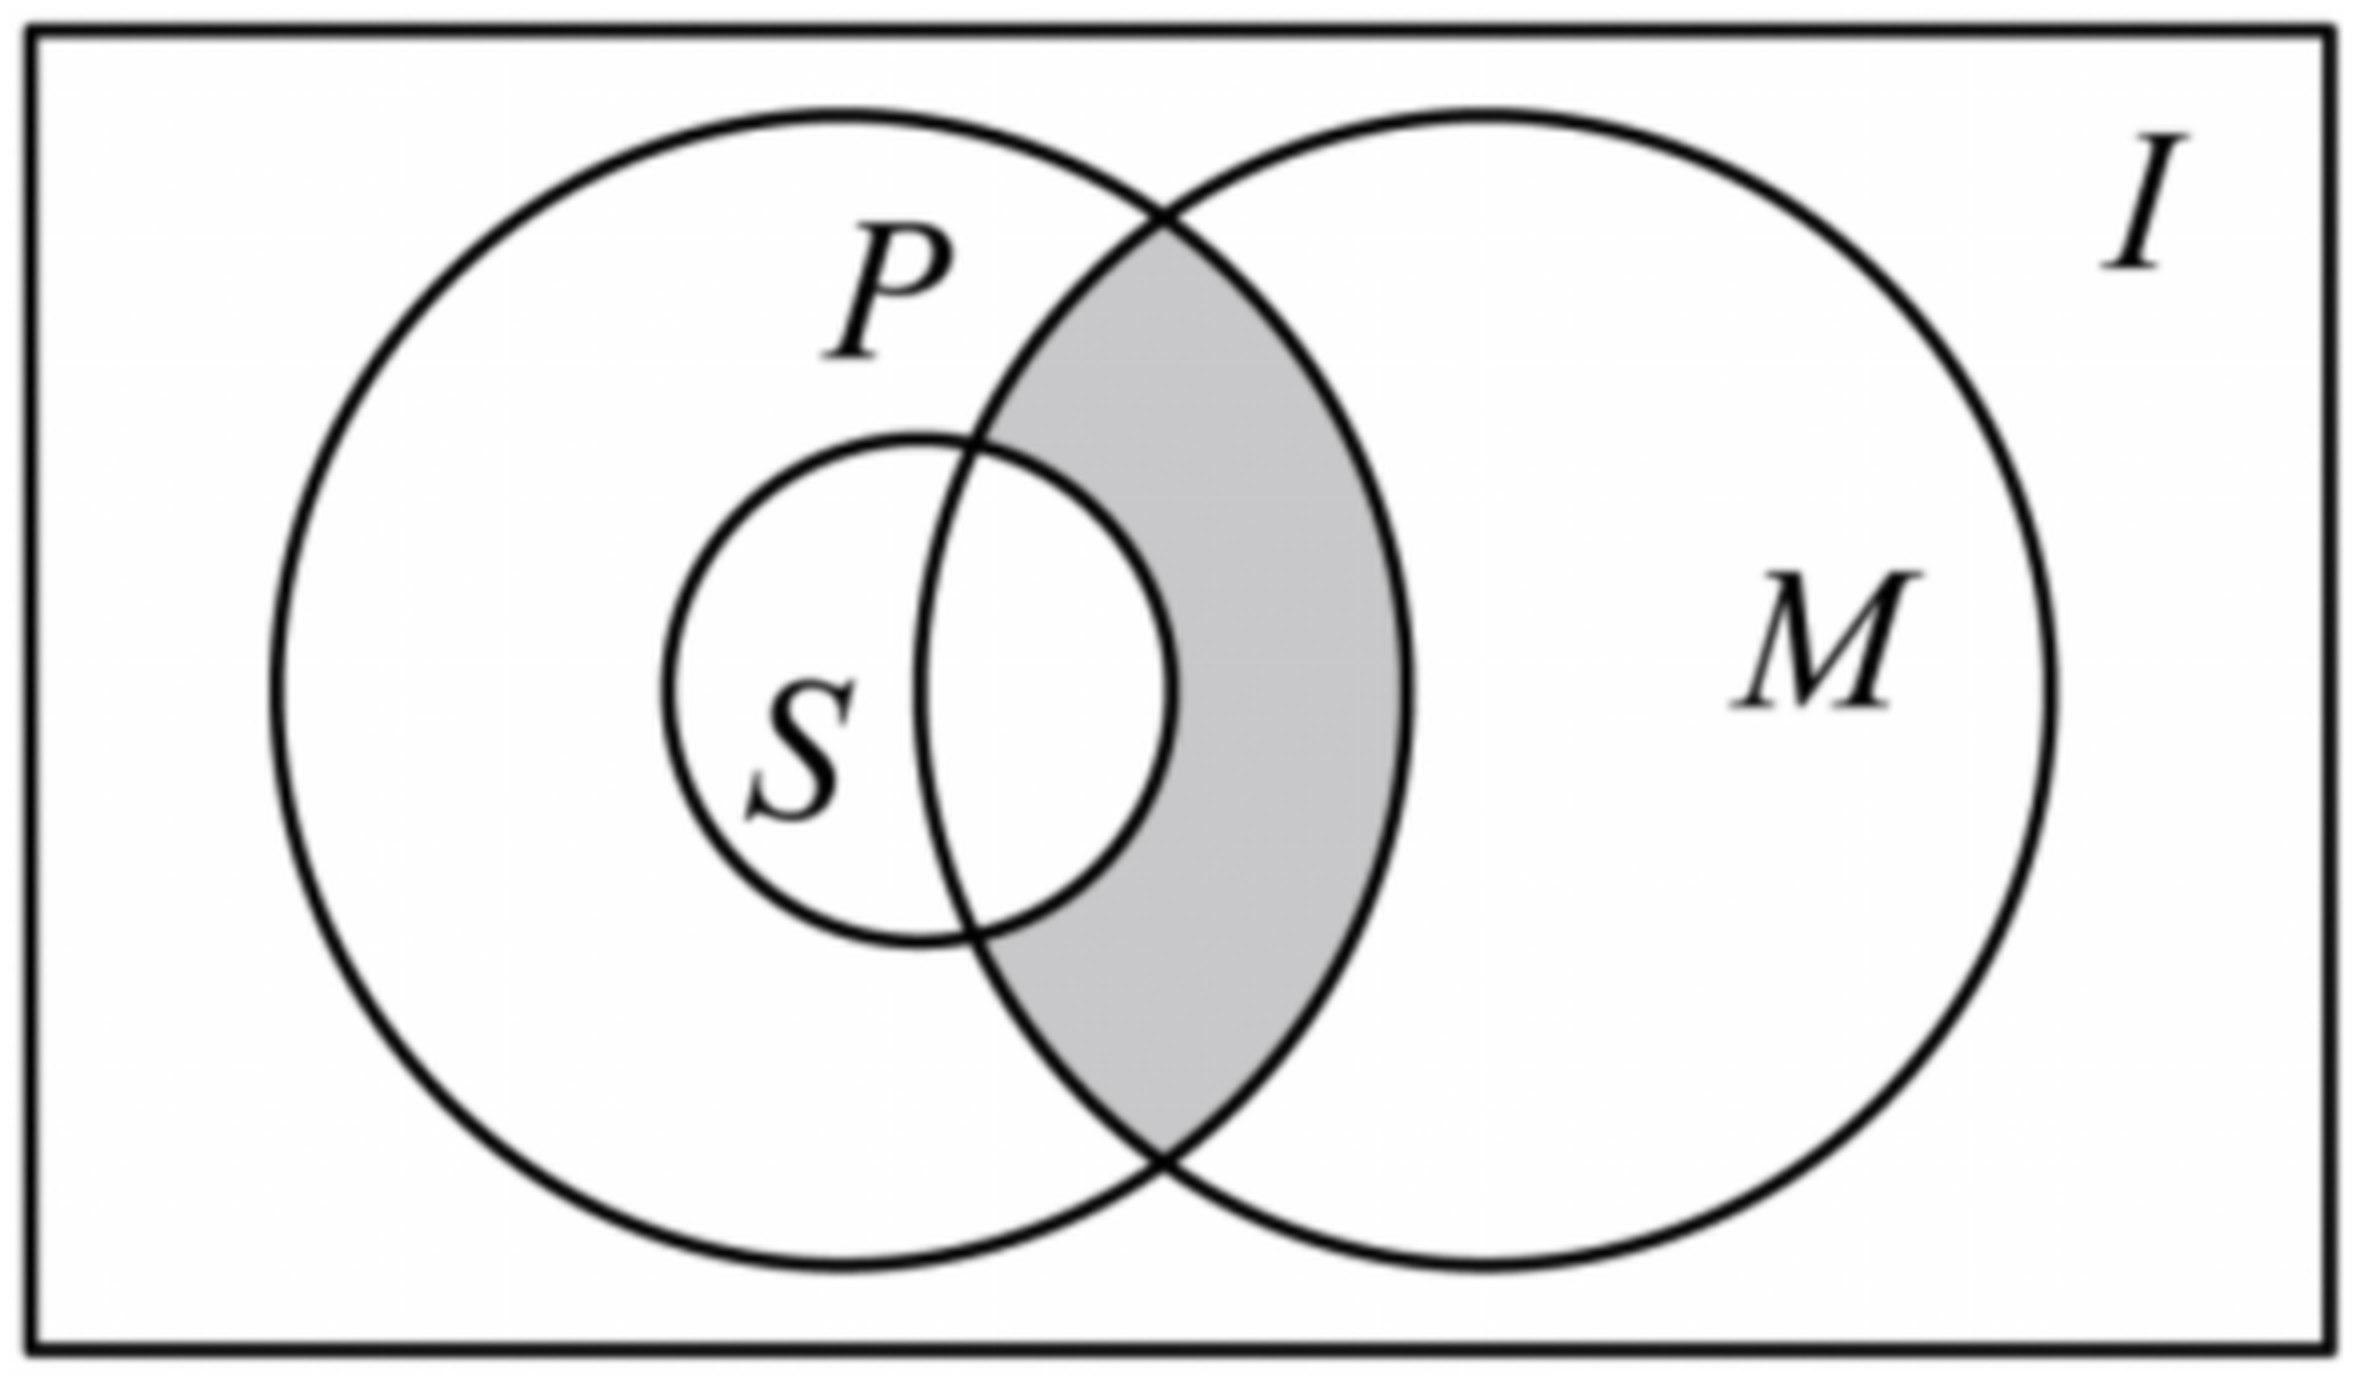
\includegraphics[width=0.46\textwidth]{figures/venn_MP_minus_S_h32.png}
\end{center}

\keepwithprev
A. $(M\cap P)\cap S$\qquad\qquad B. $(M\cap P)\cup S$

C. $(M\cap P)\cap\overline{S}$\qquad\qquad D. $(M\cap P)\cup\overline{S}$

\ans{$C$}

\ifanswer
\solbegin
\step{由 Venn 图得，集合表示 $M$、$P$ 的交集与 $S$ 的补集的交集，}
\step{即阴影部分所表示的集合是 $(M\cap P)\cap\overline{S}$. 故选 $C$.}
\solend

\fi

\item 若实数 $a$、$b$ 满足 $ab>0$，$a+2b=6$，则下列结论中错误的是\mbox{（\quad）}

\keepwithprev
A. $ab\leqslant\dfrac92$\qquad\qquad B. $a^2+4b^2\geqslant18$

C. $\dfrac1a+\dfrac2b$ 的最小值为 $\dfrac94$\qquad\qquad
D. $\dfrac{a^2}{a+1}+\dfrac{4b^2}{2b+1}$ 的最小值为 $\dfrac92$

\ans{$C$}

\ifanswer
\solbegin
\step{因为 $ab>0$，所以 $a$、$b$ 同号，又 $a+2b=6$，所以 $a$、$b$ 同正.}
\step{对于 $A$，由 $6=a+2b\geqslant2\sqrt{a\cdot2b}$ 得 $ab\leqslant\dfrac92$，故 $A$ 正确；}
\step{对于 $B$，由不等式 $\sqrt{\dfrac{m^2+n^2}2}\geqslant\dfrac{m+n}2$ 得
$\sqrt{\dfrac{a^2+(2b)^2}2}\geqslant\dfrac{a+2b}2=3$，}
\step{所以 $a^2+4b^2\geqslant18$，当且仅当 $a=2b=3$ 时取等号，故 $B$ 正确；}
\step{对于 $C$，$\dfrac1a+\dfrac2b
=\dfrac16\left(\dfrac1a+\dfrac2b\right)(a+2b)
=\dfrac16\left(5+\dfrac{2b}a+\dfrac{2a}b\right)$}
\step{$=\dfrac56+\dfrac13\left(\dfrac ba+\dfrac ab\right)
\geqslant\dfrac56+\dfrac13\times2\sqrt{\dfrac ba\cdot\dfrac ab}=\dfrac32$，}
\step{当且仅当 $\dfrac ba=\dfrac ab$，即 $a=b=2$ 时取等号，故 $C$ 错误；}
\step{对于 $D$，$\dfrac{a^2}{a+1}+\dfrac{4b^2}{2b+1}
=\dfrac{(a+1)^2-2(a+1)+1}{a+1}+\dfrac{(2b+1)^2-2(2b+1)+1}{2b+1}$}
\step{$=(a+1)-2+\dfrac1{a+1}+(2b+1)-2+\dfrac1{2b+1}
=(a+2b-2)+\dfrac1{a+1}+\dfrac1{2b+1}$}
\step{$=(6-2)+\dfrac{a+2b+2}{(a+1)(2b+1)}
=4+\dfrac8{(a+1)(2b+1)}$，}
\step{因为 $(a+1)(2b+1)\leqslant\left(\dfrac{a+1+2b+1}2\right)^2
=\left(\dfrac82\right)^2=16$，}
\step{当且仅当 $a+1=2b+1$，即 $a=2b=3$ 时取等号，}
\step{所以 $4+\dfrac8{(a+1)(2b+1)}\geqslant4+\dfrac8{16}=\dfrac92$，
故 $D$ 正确，其他几种方法同 12 题.}
\step{故选 $C$.}
\solend

\fi

% 注：本题的答案「D」原卷直接印在题干末尾的括号内，本稿按全稿惯例另提为 \ans{}。
\item 已知函数 $f(x)=x^2-2ax+a^2-1$，定义集合 $A=\{x\mid f(x)<0\}$. 若集合
$\{x\mid f(x)\in A\}=\varnothing$，则实数 $a$ 的取值范围是\mbox{（\quad）}

\keepwithprev
A. $(-3,-2)$\qquad B. $[-3,-2]$\qquad
C. $(-\infty,2)$\qquad D. $(-\infty,-2]$

\ans{$D$}

\item 非空集合 $A$ 具有如下性质：①若 $x$、$y\in A$，则 $\dfrac xy\in A$；
②若 $x$、$y\in A$，则 $x+y\in A$；

由此可知：下列判断中，错误的是\mbox{（\quad）}

\keepwithprev
A. $-1\notin A$\qquad\qquad B. $\dfrac{2025}{2026}\in A$

C. 若 $x$、$y\in A$，则 $xy\in A$\qquad\qquad
D. 若 $x$、$y\in A$，则 $x-y\in A$

\ans{$D$}

\ifanswer
\solbegin
\step{由题意得 $0\notin A$，$1\in A$，}
\step{对于 $A$，假设 $-1\in A$，则 $-1+1=0\in A$，矛盾，所以 $-1\notin A$，故 $A$ 正确；}
\step{对于 $B$，由 $1\in A$，得 $1+1=2\in A$，$2+1=3\in A$，…，$2025\in A$，$2026\in A$，}
\step{所以 $\dfrac{2025}{2026}\in A$，故 $B$ 正确；}
\step{对于 $C$，因为 $1\in A$，$x\in A$，所以 $\dfrac1x\in A$，
又因为 $y\in A$，所以 $\dfrac y{\frac1x}=xy\in A$，}
\step{故 $C$ 正确；}
\step{对于 $D$，因为 $1\in A$，$2\in A$，若 $x=1$，$y=2$，则 $x-y=-1\notin A$，故 $D$ 错误.}
\step{故选 $D$.}
\solend

\fi

\end{enumerate}

\bigsec{三、解答题}

\begin{enumerate}
\setcounter{enumi}{16}

\item 求下列关于实数 $x$ 的不等式的解集.

\begin{enumerate}[label=(\arabic*)]
\item $|2x+1|<5x-1$；
\item $\dfrac{(x-1)(x-3)(x-6)}{(x-2)(x-4)^2(x-5)}\geqslant0$.
\end{enumerate}

\ifanswer
\solbegin
\stepm{(1)}{因为不等式 $|2x+1|<5x-1$ 可化为 $-(5x-1)<2x+1<5x-1$，且 $5x-1>0$，}
\step{解得 $x>\dfrac23$，所以原不等式的解集为 $\left(\dfrac23,+\infty\right)$；}
\stepm{(2)}{不等式 $\dfrac{(x-1)(x-3)(x-6)}{(x-2)(x-4)^2(x-5)}\geqslant0$，}
\step{等价于 $(x-1)(x-3)(x-6)(x-2)(x-5)\geqslant0$，
且 $x-2\neq0$，$x-4\neq0$，$x-5\neq0$，}
\step{由“穿针引线法”，解得 $1\leqslant x<2$ 或 $3\leqslant x<4$ 或 $4<x<5$ 或 $x\geqslant6$，}
\step{所以不等式的解集为 $[1,2)\cup[3,4)\cup(4,5)\cup[6,+\infty)$.}
\solend

\fi

\ansspace[6]

\item 已知集合 $A=\left\{x\left|mx^2-mx+\dfrac{5m}2-6=0\right.\right\}\neq\varnothing$，
集合 $B=\{x\mid1<x<4$ 且 $x\in\Z\}$，$C=\{x\mid ax+3>0\}$；若 $A\cap B=A$.

\begin{enumerate}[label=(\arabic*)]
\item 求 $m$ 的取值范围.
\item 设 $m$ 的取值集合为 $D$，若 $C\cap D=\varnothing$，求 $m$ 的值及其对应 $a$ 的取值范围.
\end{enumerate}

\ans{略}

\ansspace[8]

\item 已知函数 $f(x)=x^2+(m-2)x+2m-1$.

\begin{enumerate}[label=(\arabic*)]
\item 若 $f(x)=0$ 的两根为 $x_1$、$x_2$，且 $|x_1-x_2|=2$，求实数 $m$ 的值；
\item 若函数 $y=f(x)$ 的图像在区间 $(0,1)$ 上与 $x$ 轴只有一个交点，
求实数 $m$ 的取值范围.
\end{enumerate}

\ifanswer
\solbegin
\stepm{(1)}{由题意得 $x_1+x_2=-(m-2)=2-m$，$x_1x_2=2m-1$，}
\step{由 $|x_1-x_2|=\sqrt{(x_1+x_2)^2-4x_1x_2}
=\sqrt{(2-m)^2-4(2m-1)}=2$，}
\step{化简得 $m^2-12m+4=0$，解得 $m=6\pm4\sqrt2$，故 $m=6\pm4\sqrt2$.}
\stepm{(2)}{当 $f(x)=0$ 只有一个根，且此根位于区间 $(0,1)$，}
\step{则 $\begin{cases}0<\dfrac{2-m}2<1\\[4pt]
\Delta=(m-2)^2-4(2m-1)=0\end{cases}$，
解得 $\begin{cases}0<m<2\\ m=6-2\sqrt7\text{ 或 }m=6+2\sqrt7\end{cases}$，}
\step{所以 $m=6-2\sqrt7$；}
\step{当 $f(x)=0$ 有两个根时，有一个根在区间 $(0,1)$ 内，且另一个根位于 $[0,1]$ 之外，}
\step{则 $\begin{cases}f(0)f(1)<0\\ \Delta=(m-2)^2-4(2m-1)>0\end{cases}$，
解得 $\begin{cases}\dfrac12<m<\dfrac23\\[4pt]
m<6-2\sqrt7\text{ 或 }m>6+2\sqrt7\end{cases}$，}
% 注：下一行原卷作「即 $\dfrac12<m<\dfrac32$」，按上一行方程组应为
%     $\dfrac12<m<\dfrac23$（同页最终答案也印证），照录未改，见文件头「原卷存疑」①。
\step{即 $\dfrac12<m<\dfrac32$；}
\step{当 $f(x)=0$ 有两个根位于区间 $[0,1]$ 内，且只有一个根在区间 $(0,1)$ 内，}
\step{则另一个根为 $0$ 时，得 $m=\dfrac12$，此时 $x_1+x_2=\dfrac32$，
解得另一个根 $x_2=\dfrac32>0$，故此种情况不符题意；}
\step{当 $f(x)=0$ 有两个根位于区间 $(0,1]$ 内，且只有一个根在区间 $(0,1)$ 内，}
\step{则另一个根为 $1$ 时，得 $m=\dfrac23$，此时 $x_1+x_2=\dfrac43$，
解得另一个根 $x_2=\dfrac13$，故此种情况符合题意；}
\step{综上所述，$m$ 的取值范围为
$\left(\dfrac12,\dfrac23\right]\cup\{6-2\sqrt7\}$.}
\solend

\fi

\ansspace[8]

\item 设集合 $A=\{a_1,a_2,a_3,a_4\}$，$B=\{b_1,b_2,b_3,b_4\}$，$C=\{2,3,4,6\}$，
新定义：集合 $A$ 中所有含 $k$ 个元素的子集中 $k$ 个元素之和组成的集合为“$k$ 元集和集”，
集合 $A$ 中所有含 $k$ 个元素的子集中最大元素减去剩余所有元素的和组成的集合为“$k$ 元差集”.

\begin{enumerate}[label=(\arabic*)]
\item 若 $A$ 的“$k$ 元集和集”为 $C$，求：集合 $A$.
\item 在 (1) 的条件下，若 $B$ 的“$k$ 元差集”为 $C$，求：所有满足条件的 $A\cap B$ 的真子集
个数之和.
\item 设 $b_1=a_1^2$，$b_2=a_2^2$，$b_3=a_3^2$，$b_4=a_4^2$，若 $A\cap B$ 为 $2$ 元集且
元素之和为 $10$ 且 $A$ 的“$2$ 元集和集”中最大元素不超过 $14$，求：所有满足条件的 $A$ 的
“$3$ 元差集”.
\end{enumerate}

\ifanswer
\solbegin
\stepm{(1)}{若 $A$ 的“$k$ 元集和集”为 $C$，$C=\{2,3,4,6\}$，则集合为 $\{-1,1,2,3\}$；}
\stepm{(2)}{$B$ 集合为 $\{5,3,0,-1\}$ 或 $\{9,3,1,0\}$ 或 $\{6,3,1,-1\}$，}
\step{故所有 $A\cap B$ 的真子集个数之和为 $13$；}
\stepm{(3)}{$b_1=a_1^2$，$b_2=a_2^2$，$b_3=a_3^2$，$b_4=a_4^2$，}
\step{若 $A\cap B$ 为 $2$ 元集且元素之和为 $10$，
且 $A$ 的“$2$ 元集和集”中最大元素不超过 $14$，}
% 注：下一行答案的第二个集合 $\{0,4,5,6\}$ 是 4 元集，而题问的却是「3 元差集」，
%     原卷如此，照录未改，见文件头「原卷存疑」③。
\step{则满足条件的 $A$ 的“$3$ 元差集” $\{1,3,5\}$ 或 $\{0,4,5,6\}$ 或 $\{2,4,5,8\}$.}
\solend

\fi

\ansspace[8]

\item 已知有限集 $X$、$Y$，定义集合 $X-Y=\{x\mid x\in X$ 且 $x\notin Y\}$，
$|X|$ 表示集合 $X$ 元素个数.

\begin{enumerate}[label=(\arabic*)]
\item 若 $X=\{1,2,3,4\}$，$Y=\{3,4,5\}$，写出集合 $X-Y$ 和 $Y-X$，以及
$|(X-Y)\cup(Y-X)|$ 的值；
\item 给定正整数 $n$，集合 $S=\{1,2,\cdots,n\}$，对于实数集的非空有限子集 $A$、$B$，
定义集合 $C=\{x\mid x=a+b,a\in A,b\in B\}$；

①求证：$|A-S|+|B-S|+|S-C|\geqslant1$；

②求 $|(A-S)\cup(S-A)|+|(B-S)\cup(S-B)|+|(C-S)\cup(S-C)|$ 的最小值.
\end{enumerate}

\ifanswer
\solbegin
\stepm{(1)}{由定义直接得 $X-Y=\{1,2\}$，$Y-X=\{5\}$，
$|(X-Y)\cup(Y-X)|=3$.}
% 注：下一句原卷作「显然 $|X|\geqslant0$」（按后文论证疑为 $|S|\geqslant0$），
%     照录未改，见文件头「原卷存疑」②。
\stepm{(2)}{①显然 $|X|\geqslant0$.}
\step{若 $A\cup B$ 中含有一个不在 $S$ 中的元素，则 $|A-S|+|B-S|\geqslant1$，
即 $|A-S|+|B-S|+|S-C|\geqslant1$.}
\step{若 $A\sub S$，且 $B\sub S$，则 $|A-S|=|B-S|=0$；}
\step{此时 $A$ 中最小的元素 $a\geqslant1$，$B$ 中最小的元素 $b\geqslant1$，
所以 $C$ 中最小的元素 $a+b\geqslant2$，所以 $1\notin C$.}
\step{因为 $S=\{1,2,\cdots,n\}$，所以 $|S-C|\geqslant1$，
即 $|A-S|+|B-S|+|S-C|\geqslant1$.}
\step{综上，$|A-S|+|B-S|+|S-C|\geqslant1$.}
\step{②由①得 $|A-S|+|B-S|+|S-C|\geqslant1$.}
\step{所以 $|(A-S)\cup(S-A)|+|(B-S)\cup(S-B)|+|(C-S)\cup(S-C)|$}
\step{$=|A-S|+|S-A|+|B-S|+|S-B|+|C-S|+|S-C|$}
\step{$\geqslant|S-A|+|S-B|+|C-S|+1$.}
\step{若 $A\cap S=\varnothing$，或 $B\cap S=\varnothing$，则 $|S-A|+|S-B|\geqslant n$.}
\step{若 $A\cap S\neq\varnothing$，且 $B\cap S\neq\varnothing$，
设 $A\cap S=\{a_1,a_2,\cdots,a_s\}$，$B\cap S=\{b_1,b_2,\cdots,b_t\}$，}
\step{且 $1\leqslant a_1<a_2<\cdots<a_s\leqslant n$，
$1\leqslant b_1<b_2<\cdots<b_t\leqslant n$，则 $|S-A|=n-s$，$|B-S|=n-t$.}
% 注：原卷的解析到此为止（第 10 页末），②的最小值并未给出，照录未补，
%     见文件头「原卷存疑」④。
\solend

\fi

\ansspace*[10]

\end{enumerate}

\end{document}
"
% 紧凑版：xelatex "\def\iscompact{1}% 高一32_华师大二附中_周末作业4.tex
%   —— 高一上数学「2026-2027 年华师大二附中高一上周末作业 4」（试卷版/答案版）
% 试卷版：xelatex 高一32_华师大二附中_周末作业4.tex
% 答案版：xelatex "\def\isanswer{1}\input{高一32_华师大二附中_周末作业4.tex}"
% 紧凑版：xelatex "\def\iscompact{1}\input{高一32_华师大二附中_周末作业4.tex}"
%
% 原始材料是微信公众号图文（公众号「魔都数学加油站」连载「27学年高一 32」，2026-09-25 发布，
% 原文标题「27学年高一32——2026-2027年上海市华师大二附中高一上周末作业4」），
% 正文为 10 张 PNG 页。**同一篇里各页分辨率不一致**（2560×3620 与 4762×6735 两档混排），
% 取 mmbiz.qpic.cn/<hash>/0 的原图档。原文本身就是一份**讲评版**——有的题下方印【解析】、
% 有的印【答案】，第 15 题的答案直接印在题干末尾的括号里。
% 试题文字、答案与解析均照原卷录入，未改内容。卷面的粉色斜水印属水印，未录入。
%
% ⚠ 卷首年份：本卷卷面印作「**2025-2026 年**」，与连载「27学年高一32」及公众号原文标题的
%   「2026-2027 年」**不一致**。经三人次分别把标题行裁出放大（4×—10×）独立判读，三次都读作
%   2025-2026，且校名作「华师大二附中」（无「东」字）、卷面亦无「上海市」三字。
%   按全稿「标题行照原卷」的口径，本稿照卷面排作「2025--2026 年…」——这是全稿唯一一份
%   年份不是 2026--2027 的卷子（其余 35 份均为 2026--2027）。
%
% 卷首标题：原卷印作「……年华师大二附中高一上周末作业 4」（公众号标题里的「上海市」
% 三字卷面标题行没有，本稿照卷面），年份区间按全稿惯例排 en dash，前缀照原卷保留「年」。
%
% 与原卷的排版差异（均已在 README「说明」中交代）：
%   ① 原文自**第 3 题**起（第 1、2 题未在该文中发布），故本稿题号亦自 3 起；
%   ② 原卷本就印有「一、填空题」「二、选择题」「三、解答题」三节标题，本稿照原卷分节，
%      只把标题改排成全稿统一的「大节标题」样式；
%   ③ 原卷第 6、8、9 题只印【答案】行（第 18 题的【答案】印作「略”），其余各题印【解析】，
%      第 15 题的答案直接印在题干末尾的括号内；本稿统一改为试卷版隐去、
%      答案版以 \ans{}／\ifanswer 块给出，两版彻底分离；
%   ④ 子集符号原卷两种并用：第 21(2)① 的 $A\sub S$、$B\sub S$ 带下划线，
%      第 3、10 题的 $(0,2)\subset(-\infty,3)$、$A\subset B$、$\overline{B}\subset\overline{A}$
%      作真包含，本稿分别照录为 $\sub$ 与 $\subset$；
%   ⑤ 补集符号原卷一律作上横线（$\overline{A}$、$\overline{B}$、$\overline{S}$），本稿照录；
%      空集原卷作「斜杠伸出圆外」的 $\varnothing$；
%   ⑥ 判别式记号原卷两种：第 4 题作粗体的 $\Delta$、第 11 题作细等宽的 $\triangle$，本稿照录；
%   ⑦ 数集记号原卷作斜体的 $R$、$Z$（第 4、18 题），本稿按全稿惯例统一写作 $\R$、$\Z$；
%   ⑧ 原卷填空的横线约两个字宽，本稿按全稿惯例统一排 \blankline[4.4em]；
%   ⑨ 原卷未印副标题，本稿按全稿惯例补出副标题「集合与常用逻辑用语」；
%   ⑩ 本卷只有第 13 题一图（韦恩图），原卷印在题干右侧，本稿移至题干之后；
%      图取原卷截图、4× LANCZOS 放大（figures/venn_MP_minus_S_h32.png）。
%
% 原卷存疑四处（均照抄原卷、未改，见源码中该处上方注释）：
%   ① 第 19(2)【解析】有「即 $\dfrac12<m<\dfrac32$」，按上一行的方程组应为
%      $\dfrac12<m<\dfrac23$（同页最终答案 $\left(\dfrac12,\dfrac23\right]$ 也印证）；
%   ② 第 21(2)① 首句作「显然 $|X|\geqslant0$」（按后文论证疑为 $|S|\geqslant0$）；
%   ③ 第 20(3) 的答案第二个集合 $\{0,4,5,6\}$ 是 4 元集，而题问的是「3 元差集」；
%   ④ 第 21(2)② 的解析**原卷就未写完**（第 10 页到「则 $|S-A|=n-s$，$|B-S|=n-t$」即止）。

\documentclass[a4paper,11pt]{article}
\usepackage{common}

\begin{document}

\examtitlest[3]{2025--2026 年华师大二附中高一上周末作业 4}{集合与常用逻辑用语}

\bigsec{一、填空题}

\begin{enumerate}
\setcounter{enumi}{2}

\item 设 $x$ 为实数，则“$x<3$”是“$x(x-2)<0$”的 \blankline[4.4em] 条件.

\ifanswer
\solbegin
\step{$x(x-2)<0$，解得 $0<x<2$，$(0,2)\subset(-\infty,3)$，}
\step{若 $x$ 属于“$x(x-2)<0$”，则属于“$x<3$”一定成立，即满足必要性，}
\step{若 $x$ 属于“$x<3$”，不一定满足“$x(x-2)<0$”，如 $x=-1$，即充分性不成立；}
\step{故“$x<3$”是“$x(x-2)<0$”的必要不充分条件.}
\solend

\fi

\item 若关于 $x$ 的不等式 $kx^2-kx+1>0$ 的解集为 $\R$，则实数 $k$ 的取值范围为
\blankline[4.4em].

\ifanswer
\solbegin
\step{①当 $k=0$ 时，不等式为 $1>0$ 恒成立，满足题意；}
\step{②当 $k\neq0$ 时，只要 $\begin{cases}k>0\\ \Delta=k^2-4k<0\end{cases}$，
解得 $0<k<4$；}
\step{所以不等式 $kx^2-kx+1>0$ 的解集为 $\R$，则实数 $k$ 的取值范围为 $[0,4)$.}
\solend

\fi

\item 已知 $1<a<3$，$-5<b<-2$，则 $\dfrac ab$ 的取值范围是 \blankline[4.4em].

\ifanswer
\solbegin
\step{因为 $-5<b<-2$，所以 $2<-b<5$，$\dfrac15<-\dfrac1b<\dfrac12$，又 $1<a<3$，}
\step{得 $\dfrac15<-\dfrac ab<\dfrac32$，则 $-\dfrac32<\dfrac ab<-\dfrac15$，
故 $\dfrac ab$ 的取值范围是 $\left(-\dfrac32,-\dfrac15\right)$.}
\solend

\fi

\item 关于 $x$ 的不等式 $\dfrac{ax-1}{x-a}>1$ 的解集为 $A$，且 $3\notin A$，
则实数 $a$ 的取值范围为 \blankline[4.4em].

\ans{$(-\infty,1]\cup[3,+\infty)$}

\item 若关于 $x$ 的不等式 $a\leqslant\dfrac34x^2-3x+4\leqslant b$ 的解集恰好是 $[a,b]$，
则 $b-a=$ \blankline[4.4em].

\ifanswer
\solbegin
\step{令 $f(x)=\dfrac34x^2-3x+4$，则 $f(x)$ 的对称轴为 $x=2$，}
\step{画出函数 $f(x)=\dfrac34x^2-3x+4=\dfrac34(x-2)^2+1$ 的图象，
得 $f(x)_{\min}=f(2)=1$，}
\step{由题意得 $a\leqslant1$，且 $f(a)=f(b)=b$，$a<b$，}
\step{由 $f(b)=b$ 得 $\dfrac34b^2-3b+4=b$，解得 $b=\dfrac43$（舍去）或 $b=4$，得 $b=4$，}
\step{由抛物线的对称轴为 $x=2$ 得 $a=0$，所以 $b-a=4$.}
\solend

\fi

\item 若关于 $x$ 的方程 $x^2-2kx+k+4=0$ 在 $[1,2]$ 上有解，则实数 $k$ 的取值范围为
\blankline[4.4em].

\ans{$\left[\dfrac83,5\right]$}

\item 记关于 $x$ 的方程 $x^2-2mx-2m+3=0$ 的两实根为 $x_1$、$x_2$，
则 $(x_1-2)^2+(x_2-2)^2$ 的最小值为 \blankline[4.4em].

\ans{$2$}

\item 若“$|mx^2-4x+3|\geqslant2$”的必要非充分条件是“$x\leqslant1$ 或 $x\geqslant4$”，
则实数 $m$ 的取值范围是 \blankline[4.4em].

\ifanswer
\solbegin
\step{记 $|mx^2-4x+3|\geqslant2$ 的解集为集合 $A$，
$B=\{x\mid x\leqslant1\text{ 或 }x\geqslant4\}$，}
\step{则 $\overline{A}$ 为 $|mx^2-4x+3|<2$ 的解集，$\overline{B}=\{x\mid1<x<4\}$；}
\step{因为 $B$ 是 $A$ 的必要非充分条件，所以 $A\subset B$，
得 $\overline{B}\subset\overline{A}$，}
\step{即对任意 $x\in(1,4)$，都有 $|mx^2-4x+3|<2$ 恒成立.}
\step{因为 $|mx^2-4x+3|<2$，$1<x<4$，所以 $-2<mx^2-4x+3<2$，}
\step{化简得
$-5\left(\dfrac1x\right)^2+4\left(\dfrac1x\right)
<m<-\left(\dfrac1x\right)^2+4\left(\dfrac1x\right)$；}
\step{令 $t=\dfrac1x$，$g(t)=-5t^2+4t$，$h(t)=-t^2+4t$，
且 $t\in\left(\dfrac14,1\right)$；}
\step{所以 $g(t)=-5t^2+4t=-5\left(t-\dfrac25\right)^2+\dfrac45$，
当 $t=\dfrac25$ 时，$g(t)$ 取得最大值 $\dfrac45$，}
\step{$h(t)=-t^2+4t=-(t-2)^2+4$，当 $t=\dfrac14$ 时，$h(t)$ 取得最小值，
即 $h(t)>h\left(\dfrac14\right)=\dfrac{15}{16}$；}
\step{因为对任意 $t\in\left(\dfrac14,1\right)$，$g(t)<m<h(t)$ 恒成立，
所以 $g\left(\dfrac25\right)<m\leqslant h\left(\dfrac14\right)$，}
\step{即 $\dfrac45<m\leqslant\dfrac{15}{16}$，
所以 $m$ 的取值范围是 $\left(\dfrac45,\dfrac{15}{16}\right]$.}
\solend

\fi

\item 已知关于 $x$ 的方程 $x^2+2(m-2)x+m^2-3m+3=0$ 有两个不相等的实数根 $x_1$、$x_2$，则

$\dfrac{mx_1}{x_1-1}+\dfrac{mx_2}{x_2-1}-\dfrac2{x_1+x_2-2}$ 的最大值为 \blankline[4.4em].

\ifanswer
\solbegin
\step{关于 $x$ 的方程 $x^2+2(m-2)x+m^2-3m+3=0$ 有两个不相等的实数根 $x_1$、$x_2$，}
\step{则 $\triangle=4(m-2)^2-4(m^2-3m+3)=-4m+4>0$，得 $m<1$，}
\step{且 $x_1+x_2=-2(m-2)$，$x_1x_2=m^2-3m+3$，}
\step{$\dfrac{mx_1}{x_1-1}+\dfrac{mx_2}{x_2-1}-\dfrac2{x_1+x_2-2}
=\dfrac{m[2x_1x_2-(x_1+x_2)]}{x_1x_2-(x_1+x_2)+1}+\dfrac1{m-1}$}
\step{$=\dfrac{2m(m-1)^2}{m^2-m}+\dfrac1{m-1}=2(m-1)+\dfrac1{m-1}$，}
\step{又因为 $m<1$，所以 $m-1<0$，则 $1-m>0$，}
\step{所以 $2(1-m)+\dfrac1{1-m}\geqslant2\sqrt{2(1-m)\cdot\dfrac1{1-m}}=2\sqrt2$，}
\step{当且仅当 $2(1-m)=\dfrac1{1-m}$ 时，即 $m=1-\dfrac{\sqrt2}2$ 时取等号，}
\step{所以 $2(m-1)+\dfrac1{m-1}\leqslant-2\sqrt2$，
即 $\dfrac{mx_1}{x_1-1}+\dfrac{mx_2}{x_2-1}-\dfrac2{x_1+x_2-2}$ 的最大值为 $-2\sqrt2$.}
\solend

\fi

\item 若正实数 $a$、$b$ 满足 $a+2b=ab$，则 $\dfrac4{a^2+2a}+\dfrac1{2b^2+b}$ 的最小值是
\blankline[4.4em].

\ifanswer
\solbegin
\stepm{法一}{由 $a+2b=ab$，得 $\dfrac2a+\dfrac1b=1$，}
\step{令 $x=\dfrac1a$，$y=\dfrac1b$，则 $x$、$y>0$，$2x+y=1$，$2x+1+y+2=4$，}
\step{所以 $\dfrac4{a^2+2a}+\dfrac1{2b^2+b}
=\dfrac4{\frac1{x^2}+\frac2x}+\dfrac1{\frac2{y^2}+\frac1y}
=\dfrac{4x^2}{2x+1}+\dfrac{y^2}{y+2}$（*）}
\step{$=\dfrac{(2x+1)^2-2(2x+1)+1}{2x+1}+\dfrac{(y+2)^2-4(y+2)+4}{y+2}$}
\step{$=2x-1+\dfrac1{2x+1}+y-2+\dfrac4{y+2}=\dfrac1{2x+1}+\dfrac4{y+2}-2$}
\step{$=\dfrac14\left(\dfrac1{2x+1}+\dfrac4{y+2}\right)(2x+1+y+2)-2$}
\step{$=\dfrac14\left[5+\dfrac{y+2}{2x+1}+\dfrac{4(2x+1)}{y+2}\right]-2
\geqslant\dfrac14(5+2\sqrt4)-2=\dfrac14$，}
\step{当且仅当 $\dfrac{y+2}{2x+1}=\dfrac{4(2x+1)}{y+2}$，
即 $x=\dfrac16$，$y=\dfrac23$ 时取等号，}
\step{故 $\dfrac4{a^2+2a}+\dfrac1{2b^2+b}$ 的最小值是 $\dfrac14$.}
\stepm{法二}{在法一（*）后，由权方和不等式，得
$\dfrac4{a^2+2a}+\dfrac1{2b^2+b}
=\dfrac{4x^2}{2x+1}+\dfrac{y^2}{y+2}
\geqslant\dfrac{(2x+y)^2}{2x+1+y+2}=\dfrac14$，}
\step{当且仅当……，故 $\dfrac4{a^2+2a}+\dfrac1{2b^2+b}$ 的最小值是 $\dfrac14$.}
\stepm{法三}{注意到
$\left(\dfrac{a+2}a+\dfrac{2b+1}b\right)\left(\dfrac4{a^2+2a}+\dfrac1{2b^2+b}\right)$}
\step{$\geqslant
\left(\sqrt{\dfrac{a+2}a\cdot\dfrac4{a^2+2a}}
+\sqrt{\dfrac{2b+1}b\cdot\dfrac1{2b^2+b}}\right)^2
=\left(\dfrac2a+\dfrac1b\right)^2$，}
\step{其中 $\dfrac{a+2}a+\dfrac{2b+1}b=3+\dfrac{a+2b}{ab}=4$，
$\dfrac2a+\dfrac1b=\dfrac{a+2b}{ab}=1$，}
\step{所以 $\dfrac4{a^2+2a}+\dfrac1{2b^2+b}\geqslant\dfrac14$，
当且仅当……，故 $\dfrac4{a^2+2a}+\dfrac1{2b^2+b}$ 的最小值是 $\dfrac14$.}
\solend

\fi

\end{enumerate}

\bigsec{二、选择题}

\begin{enumerate}
\setcounter{enumi}{12}

\item 如图，$I$ 为全集，$M$、$P$、$S$ 是 $I$ 的三个子集，则阴影部分所表示的集合是
\mbox{（\quad）}

\begin{center}
% 图取原卷截图、4× LANCZOS 放大（原卷把图印在题干右侧，本稿移至此处，见文件头⑩）。
% 矩形为全集 $I$，左大圆 $P$（内下方含小圆 $S$，其右侧伸入 $P$ 与 $M$ 的重叠区）、
% 右大圆 $M$；阴影是 $P$、$M$ 重叠的透镜形区域挖掉 $S$ 后剩下的部分（左缘呈弯月形）。
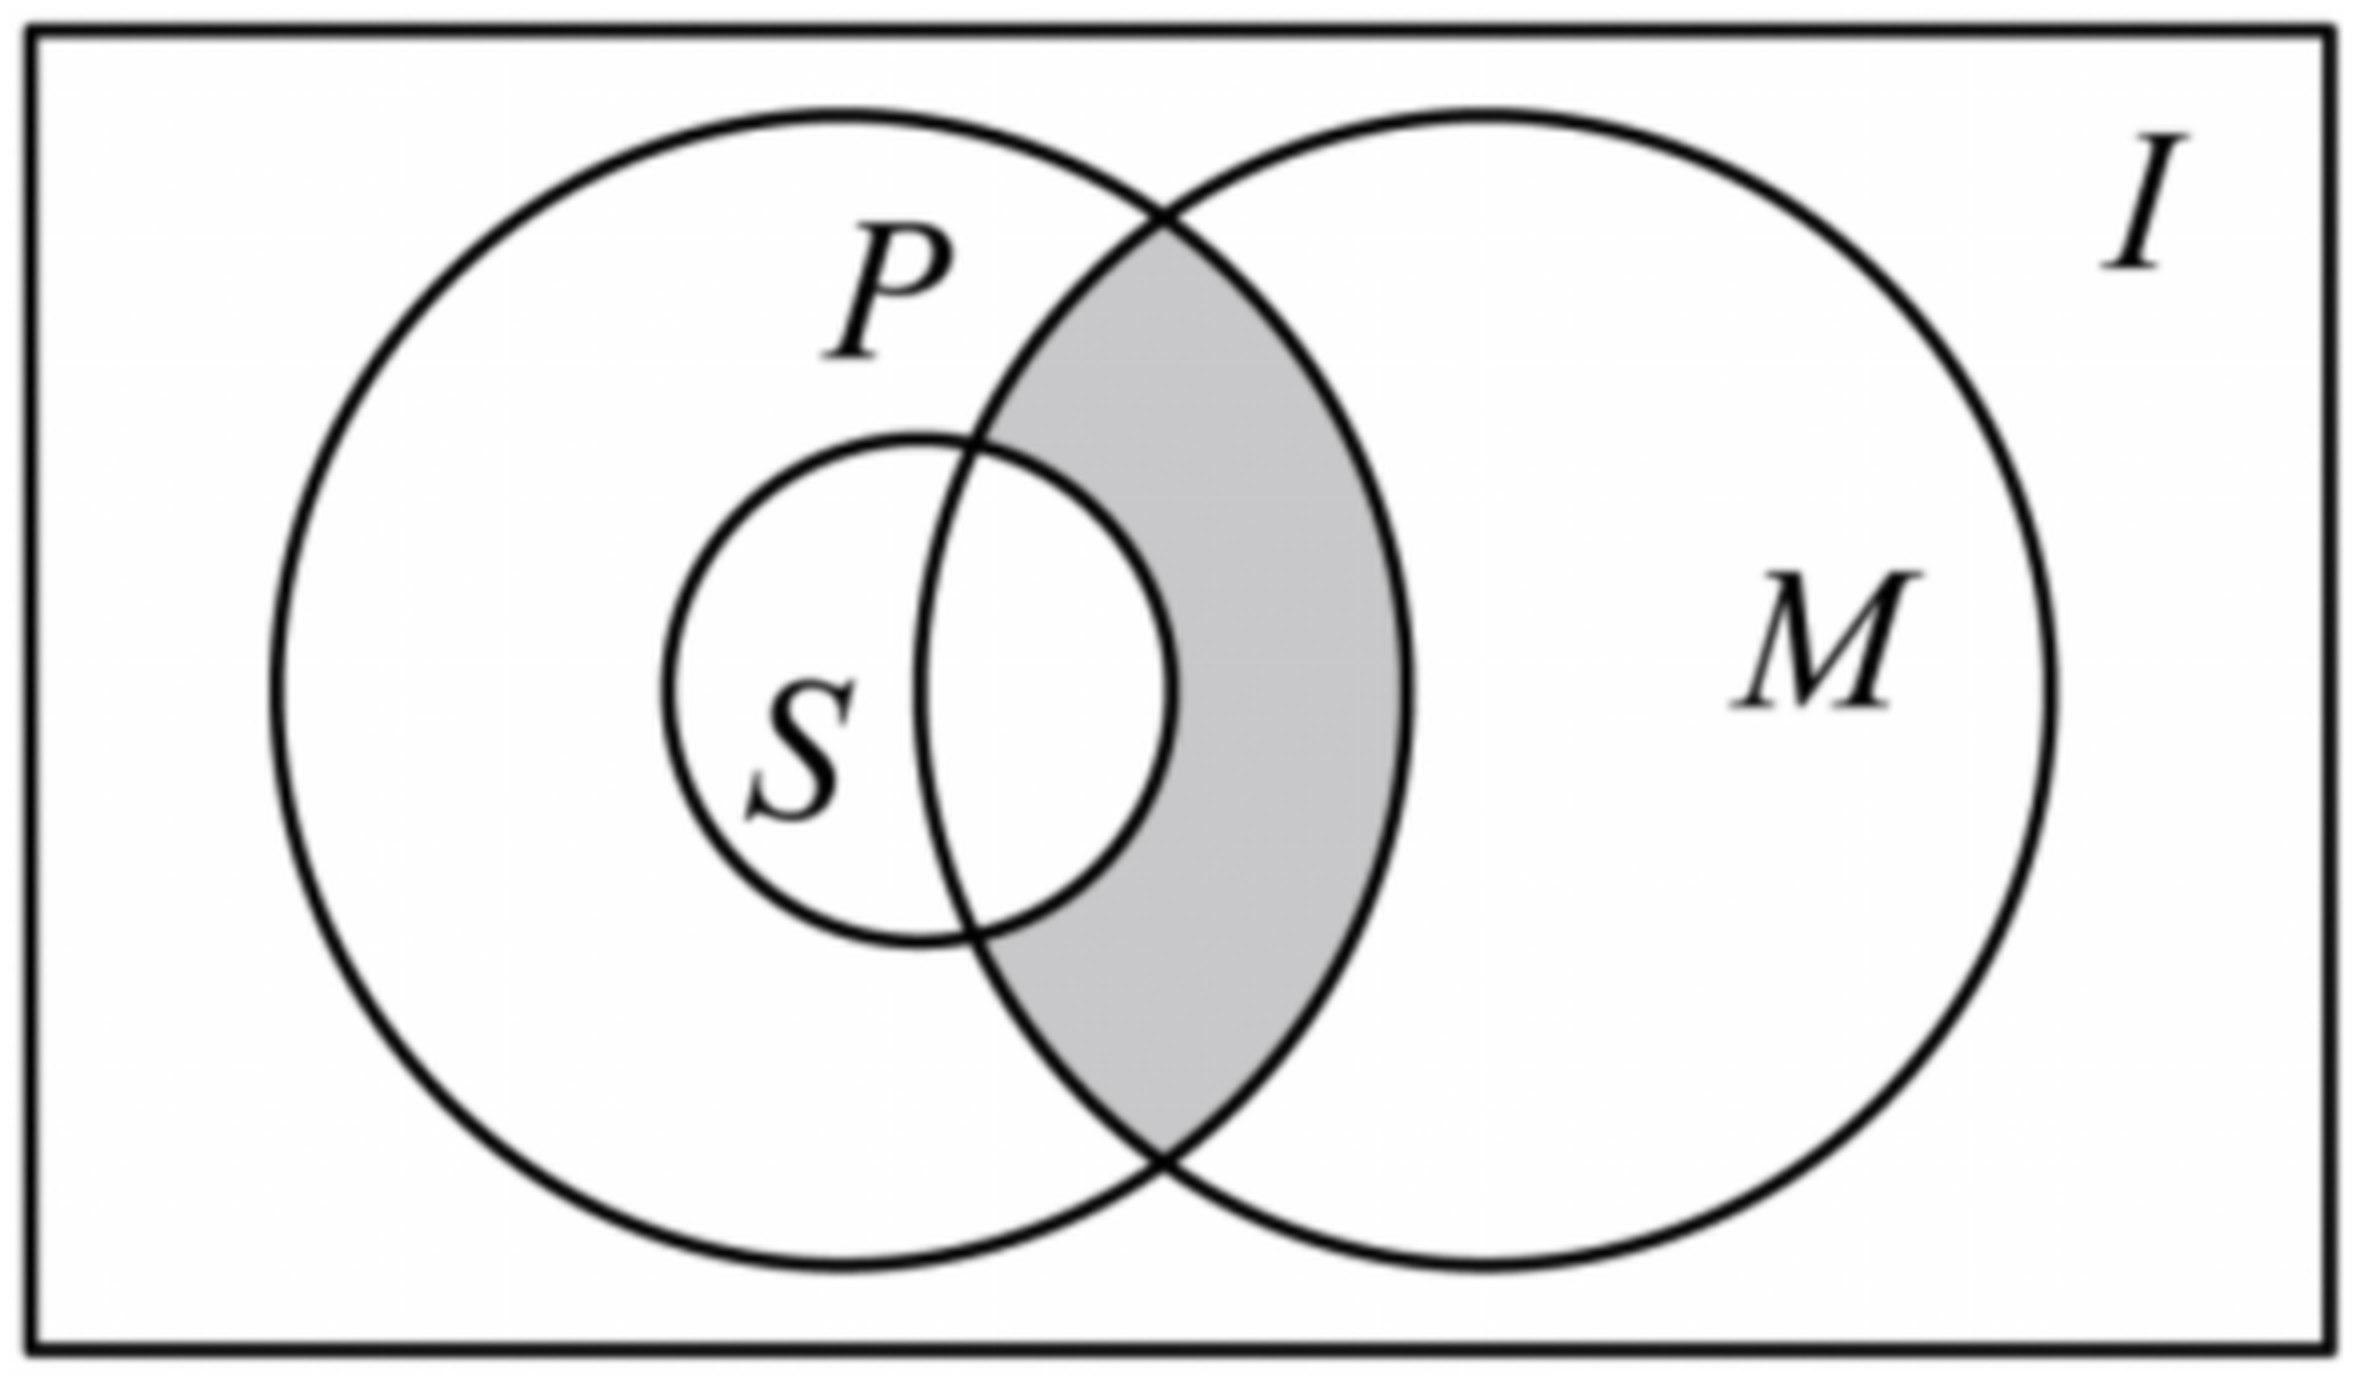
\includegraphics[width=0.46\textwidth]{figures/venn_MP_minus_S_h32.png}
\end{center}

\keepwithprev
A. $(M\cap P)\cap S$\qquad\qquad B. $(M\cap P)\cup S$

C. $(M\cap P)\cap\overline{S}$\qquad\qquad D. $(M\cap P)\cup\overline{S}$

\ans{$C$}

\ifanswer
\solbegin
\step{由 Venn 图得，集合表示 $M$、$P$ 的交集与 $S$ 的补集的交集，}
\step{即阴影部分所表示的集合是 $(M\cap P)\cap\overline{S}$. 故选 $C$.}
\solend

\fi

\item 若实数 $a$、$b$ 满足 $ab>0$，$a+2b=6$，则下列结论中错误的是\mbox{（\quad）}

\keepwithprev
A. $ab\leqslant\dfrac92$\qquad\qquad B. $a^2+4b^2\geqslant18$

C. $\dfrac1a+\dfrac2b$ 的最小值为 $\dfrac94$\qquad\qquad
D. $\dfrac{a^2}{a+1}+\dfrac{4b^2}{2b+1}$ 的最小值为 $\dfrac92$

\ans{$C$}

\ifanswer
\solbegin
\step{因为 $ab>0$，所以 $a$、$b$ 同号，又 $a+2b=6$，所以 $a$、$b$ 同正.}
\step{对于 $A$，由 $6=a+2b\geqslant2\sqrt{a\cdot2b}$ 得 $ab\leqslant\dfrac92$，故 $A$ 正确；}
\step{对于 $B$，由不等式 $\sqrt{\dfrac{m^2+n^2}2}\geqslant\dfrac{m+n}2$ 得
$\sqrt{\dfrac{a^2+(2b)^2}2}\geqslant\dfrac{a+2b}2=3$，}
\step{所以 $a^2+4b^2\geqslant18$，当且仅当 $a=2b=3$ 时取等号，故 $B$ 正确；}
\step{对于 $C$，$\dfrac1a+\dfrac2b
=\dfrac16\left(\dfrac1a+\dfrac2b\right)(a+2b)
=\dfrac16\left(5+\dfrac{2b}a+\dfrac{2a}b\right)$}
\step{$=\dfrac56+\dfrac13\left(\dfrac ba+\dfrac ab\right)
\geqslant\dfrac56+\dfrac13\times2\sqrt{\dfrac ba\cdot\dfrac ab}=\dfrac32$，}
\step{当且仅当 $\dfrac ba=\dfrac ab$，即 $a=b=2$ 时取等号，故 $C$ 错误；}
\step{对于 $D$，$\dfrac{a^2}{a+1}+\dfrac{4b^2}{2b+1}
=\dfrac{(a+1)^2-2(a+1)+1}{a+1}+\dfrac{(2b+1)^2-2(2b+1)+1}{2b+1}$}
\step{$=(a+1)-2+\dfrac1{a+1}+(2b+1)-2+\dfrac1{2b+1}
=(a+2b-2)+\dfrac1{a+1}+\dfrac1{2b+1}$}
\step{$=(6-2)+\dfrac{a+2b+2}{(a+1)(2b+1)}
=4+\dfrac8{(a+1)(2b+1)}$，}
\step{因为 $(a+1)(2b+1)\leqslant\left(\dfrac{a+1+2b+1}2\right)^2
=\left(\dfrac82\right)^2=16$，}
\step{当且仅当 $a+1=2b+1$，即 $a=2b=3$ 时取等号，}
\step{所以 $4+\dfrac8{(a+1)(2b+1)}\geqslant4+\dfrac8{16}=\dfrac92$，
故 $D$ 正确，其他几种方法同 12 题.}
\step{故选 $C$.}
\solend

\fi

% 注：本题的答案「D」原卷直接印在题干末尾的括号内，本稿按全稿惯例另提为 \ans{}。
\item 已知函数 $f(x)=x^2-2ax+a^2-1$，定义集合 $A=\{x\mid f(x)<0\}$. 若集合
$\{x\mid f(x)\in A\}=\varnothing$，则实数 $a$ 的取值范围是\mbox{（\quad）}

\keepwithprev
A. $(-3,-2)$\qquad B. $[-3,-2]$\qquad
C. $(-\infty,2)$\qquad D. $(-\infty,-2]$

\ans{$D$}

\item 非空集合 $A$ 具有如下性质：①若 $x$、$y\in A$，则 $\dfrac xy\in A$；
②若 $x$、$y\in A$，则 $x+y\in A$；

由此可知：下列判断中，错误的是\mbox{（\quad）}

\keepwithprev
A. $-1\notin A$\qquad\qquad B. $\dfrac{2025}{2026}\in A$

C. 若 $x$、$y\in A$，则 $xy\in A$\qquad\qquad
D. 若 $x$、$y\in A$，则 $x-y\in A$

\ans{$D$}

\ifanswer
\solbegin
\step{由题意得 $0\notin A$，$1\in A$，}
\step{对于 $A$，假设 $-1\in A$，则 $-1+1=0\in A$，矛盾，所以 $-1\notin A$，故 $A$ 正确；}
\step{对于 $B$，由 $1\in A$，得 $1+1=2\in A$，$2+1=3\in A$，…，$2025\in A$，$2026\in A$，}
\step{所以 $\dfrac{2025}{2026}\in A$，故 $B$ 正确；}
\step{对于 $C$，因为 $1\in A$，$x\in A$，所以 $\dfrac1x\in A$，
又因为 $y\in A$，所以 $\dfrac y{\frac1x}=xy\in A$，}
\step{故 $C$ 正确；}
\step{对于 $D$，因为 $1\in A$，$2\in A$，若 $x=1$，$y=2$，则 $x-y=-1\notin A$，故 $D$ 错误.}
\step{故选 $D$.}
\solend

\fi

\end{enumerate}

\bigsec{三、解答题}

\begin{enumerate}
\setcounter{enumi}{16}

\item 求下列关于实数 $x$ 的不等式的解集.

\begin{enumerate}[label=(\arabic*)]
\item $|2x+1|<5x-1$；
\item $\dfrac{(x-1)(x-3)(x-6)}{(x-2)(x-4)^2(x-5)}\geqslant0$.
\end{enumerate}

\ifanswer
\solbegin
\stepm{(1)}{因为不等式 $|2x+1|<5x-1$ 可化为 $-(5x-1)<2x+1<5x-1$，且 $5x-1>0$，}
\step{解得 $x>\dfrac23$，所以原不等式的解集为 $\left(\dfrac23,+\infty\right)$；}
\stepm{(2)}{不等式 $\dfrac{(x-1)(x-3)(x-6)}{(x-2)(x-4)^2(x-5)}\geqslant0$，}
\step{等价于 $(x-1)(x-3)(x-6)(x-2)(x-5)\geqslant0$，
且 $x-2\neq0$，$x-4\neq0$，$x-5\neq0$，}
\step{由“穿针引线法”，解得 $1\leqslant x<2$ 或 $3\leqslant x<4$ 或 $4<x<5$ 或 $x\geqslant6$，}
\step{所以不等式的解集为 $[1,2)\cup[3,4)\cup(4,5)\cup[6,+\infty)$.}
\solend

\fi

\ansspace[6]

\item 已知集合 $A=\left\{x\left|mx^2-mx+\dfrac{5m}2-6=0\right.\right\}\neq\varnothing$，
集合 $B=\{x\mid1<x<4$ 且 $x\in\Z\}$，$C=\{x\mid ax+3>0\}$；若 $A\cap B=A$.

\begin{enumerate}[label=(\arabic*)]
\item 求 $m$ 的取值范围.
\item 设 $m$ 的取值集合为 $D$，若 $C\cap D=\varnothing$，求 $m$ 的值及其对应 $a$ 的取值范围.
\end{enumerate}

\ans{略}

\ansspace[8]

\item 已知函数 $f(x)=x^2+(m-2)x+2m-1$.

\begin{enumerate}[label=(\arabic*)]
\item 若 $f(x)=0$ 的两根为 $x_1$、$x_2$，且 $|x_1-x_2|=2$，求实数 $m$ 的值；
\item 若函数 $y=f(x)$ 的图像在区间 $(0,1)$ 上与 $x$ 轴只有一个交点，
求实数 $m$ 的取值范围.
\end{enumerate}

\ifanswer
\solbegin
\stepm{(1)}{由题意得 $x_1+x_2=-(m-2)=2-m$，$x_1x_2=2m-1$，}
\step{由 $|x_1-x_2|=\sqrt{(x_1+x_2)^2-4x_1x_2}
=\sqrt{(2-m)^2-4(2m-1)}=2$，}
\step{化简得 $m^2-12m+4=0$，解得 $m=6\pm4\sqrt2$，故 $m=6\pm4\sqrt2$.}
\stepm{(2)}{当 $f(x)=0$ 只有一个根，且此根位于区间 $(0,1)$，}
\step{则 $\begin{cases}0<\dfrac{2-m}2<1\\[4pt]
\Delta=(m-2)^2-4(2m-1)=0\end{cases}$，
解得 $\begin{cases}0<m<2\\ m=6-2\sqrt7\text{ 或 }m=6+2\sqrt7\end{cases}$，}
\step{所以 $m=6-2\sqrt7$；}
\step{当 $f(x)=0$ 有两个根时，有一个根在区间 $(0,1)$ 内，且另一个根位于 $[0,1]$ 之外，}
\step{则 $\begin{cases}f(0)f(1)<0\\ \Delta=(m-2)^2-4(2m-1)>0\end{cases}$，
解得 $\begin{cases}\dfrac12<m<\dfrac23\\[4pt]
m<6-2\sqrt7\text{ 或 }m>6+2\sqrt7\end{cases}$，}
% 注：下一行原卷作「即 $\dfrac12<m<\dfrac32$」，按上一行方程组应为
%     $\dfrac12<m<\dfrac23$（同页最终答案也印证），照录未改，见文件头「原卷存疑」①。
\step{即 $\dfrac12<m<\dfrac32$；}
\step{当 $f(x)=0$ 有两个根位于区间 $[0,1]$ 内，且只有一个根在区间 $(0,1)$ 内，}
\step{则另一个根为 $0$ 时，得 $m=\dfrac12$，此时 $x_1+x_2=\dfrac32$，
解得另一个根 $x_2=\dfrac32>0$，故此种情况不符题意；}
\step{当 $f(x)=0$ 有两个根位于区间 $(0,1]$ 内，且只有一个根在区间 $(0,1)$ 内，}
\step{则另一个根为 $1$ 时，得 $m=\dfrac23$，此时 $x_1+x_2=\dfrac43$，
解得另一个根 $x_2=\dfrac13$，故此种情况符合题意；}
\step{综上所述，$m$ 的取值范围为
$\left(\dfrac12,\dfrac23\right]\cup\{6-2\sqrt7\}$.}
\solend

\fi

\ansspace[8]

\item 设集合 $A=\{a_1,a_2,a_3,a_4\}$，$B=\{b_1,b_2,b_3,b_4\}$，$C=\{2,3,4,6\}$，
新定义：集合 $A$ 中所有含 $k$ 个元素的子集中 $k$ 个元素之和组成的集合为“$k$ 元集和集”，
集合 $A$ 中所有含 $k$ 个元素的子集中最大元素减去剩余所有元素的和组成的集合为“$k$ 元差集”.

\begin{enumerate}[label=(\arabic*)]
\item 若 $A$ 的“$k$ 元集和集”为 $C$，求：集合 $A$.
\item 在 (1) 的条件下，若 $B$ 的“$k$ 元差集”为 $C$，求：所有满足条件的 $A\cap B$ 的真子集
个数之和.
\item 设 $b_1=a_1^2$，$b_2=a_2^2$，$b_3=a_3^2$，$b_4=a_4^2$，若 $A\cap B$ 为 $2$ 元集且
元素之和为 $10$ 且 $A$ 的“$2$ 元集和集”中最大元素不超过 $14$，求：所有满足条件的 $A$ 的
“$3$ 元差集”.
\end{enumerate}

\ifanswer
\solbegin
\stepm{(1)}{若 $A$ 的“$k$ 元集和集”为 $C$，$C=\{2,3,4,6\}$，则集合为 $\{-1,1,2,3\}$；}
\stepm{(2)}{$B$ 集合为 $\{5,3,0,-1\}$ 或 $\{9,3,1,0\}$ 或 $\{6,3,1,-1\}$，}
\step{故所有 $A\cap B$ 的真子集个数之和为 $13$；}
\stepm{(3)}{$b_1=a_1^2$，$b_2=a_2^2$，$b_3=a_3^2$，$b_4=a_4^2$，}
\step{若 $A\cap B$ 为 $2$ 元集且元素之和为 $10$，
且 $A$ 的“$2$ 元集和集”中最大元素不超过 $14$，}
% 注：下一行答案的第二个集合 $\{0,4,5,6\}$ 是 4 元集，而题问的却是「3 元差集」，
%     原卷如此，照录未改，见文件头「原卷存疑」③。
\step{则满足条件的 $A$ 的“$3$ 元差集” $\{1,3,5\}$ 或 $\{0,4,5,6\}$ 或 $\{2,4,5,8\}$.}
\solend

\fi

\ansspace[8]

\item 已知有限集 $X$、$Y$，定义集合 $X-Y=\{x\mid x\in X$ 且 $x\notin Y\}$，
$|X|$ 表示集合 $X$ 元素个数.

\begin{enumerate}[label=(\arabic*)]
\item 若 $X=\{1,2,3,4\}$，$Y=\{3,4,5\}$，写出集合 $X-Y$ 和 $Y-X$，以及
$|(X-Y)\cup(Y-X)|$ 的值；
\item 给定正整数 $n$，集合 $S=\{1,2,\cdots,n\}$，对于实数集的非空有限子集 $A$、$B$，
定义集合 $C=\{x\mid x=a+b,a\in A,b\in B\}$；

①求证：$|A-S|+|B-S|+|S-C|\geqslant1$；

②求 $|(A-S)\cup(S-A)|+|(B-S)\cup(S-B)|+|(C-S)\cup(S-C)|$ 的最小值.
\end{enumerate}

\ifanswer
\solbegin
\stepm{(1)}{由定义直接得 $X-Y=\{1,2\}$，$Y-X=\{5\}$，
$|(X-Y)\cup(Y-X)|=3$.}
% 注：下一句原卷作「显然 $|X|\geqslant0$」（按后文论证疑为 $|S|\geqslant0$），
%     照录未改，见文件头「原卷存疑」②。
\stepm{(2)}{①显然 $|X|\geqslant0$.}
\step{若 $A\cup B$ 中含有一个不在 $S$ 中的元素，则 $|A-S|+|B-S|\geqslant1$，
即 $|A-S|+|B-S|+|S-C|\geqslant1$.}
\step{若 $A\sub S$，且 $B\sub S$，则 $|A-S|=|B-S|=0$；}
\step{此时 $A$ 中最小的元素 $a\geqslant1$，$B$ 中最小的元素 $b\geqslant1$，
所以 $C$ 中最小的元素 $a+b\geqslant2$，所以 $1\notin C$.}
\step{因为 $S=\{1,2,\cdots,n\}$，所以 $|S-C|\geqslant1$，
即 $|A-S|+|B-S|+|S-C|\geqslant1$.}
\step{综上，$|A-S|+|B-S|+|S-C|\geqslant1$.}
\step{②由①得 $|A-S|+|B-S|+|S-C|\geqslant1$.}
\step{所以 $|(A-S)\cup(S-A)|+|(B-S)\cup(S-B)|+|(C-S)\cup(S-C)|$}
\step{$=|A-S|+|S-A|+|B-S|+|S-B|+|C-S|+|S-C|$}
\step{$\geqslant|S-A|+|S-B|+|C-S|+1$.}
\step{若 $A\cap S=\varnothing$，或 $B\cap S=\varnothing$，则 $|S-A|+|S-B|\geqslant n$.}
\step{若 $A\cap S\neq\varnothing$，且 $B\cap S\neq\varnothing$，
设 $A\cap S=\{a_1,a_2,\cdots,a_s\}$，$B\cap S=\{b_1,b_2,\cdots,b_t\}$，}
\step{且 $1\leqslant a_1<a_2<\cdots<a_s\leqslant n$，
$1\leqslant b_1<b_2<\cdots<b_t\leqslant n$，则 $|S-A|=n-s$，$|B-S|=n-t$.}
% 注：原卷的解析到此为止（第 10 页末），②的最小值并未给出，照录未补，
%     见文件头「原卷存疑」④。
\solend

\fi

\ansspace*[10]

\end{enumerate}

\end{document}
"
%
% 原始材料是微信公众号图文（公众号「魔都数学加油站」连载「27学年高一 32」，2026-09-25 发布，
% 原文标题「27学年高一32——2026-2027年上海市华师大二附中高一上周末作业4」），
% 正文为 10 张 PNG 页。**同一篇里各页分辨率不一致**（2560×3620 与 4762×6735 两档混排），
% 取 mmbiz.qpic.cn/<hash>/0 的原图档。原文本身就是一份**讲评版**——有的题下方印【解析】、
% 有的印【答案】，第 15 题的答案直接印在题干末尾的括号里。
% 试题文字、答案与解析均照原卷录入，未改内容。卷面的粉色斜水印属水印，未录入。
%
% ⚠ 卷首年份：本卷卷面印作「**2025-2026 年**」，与连载「27学年高一32」及公众号原文标题的
%   「2026-2027 年」**不一致**。经三人次分别把标题行裁出放大（4×—10×）独立判读，三次都读作
%   2025-2026，且校名作「华师大二附中」（无「东」字）、卷面亦无「上海市」三字。
%   按全稿「标题行照原卷」的口径，本稿照卷面排作「2025--2026 年…」——这是全稿唯一一份
%   年份不是 2026--2027 的卷子（其余 35 份均为 2026--2027）。
%
% 卷首标题：原卷印作「……年华师大二附中高一上周末作业 4」（公众号标题里的「上海市」
% 三字卷面标题行没有，本稿照卷面），年份区间按全稿惯例排 en dash，前缀照原卷保留「年」。
%
% 与原卷的排版差异（均已在 README「说明」中交代）：
%   ① 原文自**第 3 题**起（第 1、2 题未在该文中发布），故本稿题号亦自 3 起；
%   ② 原卷本就印有「一、填空题」「二、选择题」「三、解答题」三节标题，本稿照原卷分节，
%      只把标题改排成全稿统一的「大节标题」样式；
%   ③ 原卷第 6、8、9 题只印【答案】行（第 18 题的【答案】印作「略”），其余各题印【解析】，
%      第 15 题的答案直接印在题干末尾的括号内；本稿统一改为试卷版隐去、
%      答案版以 \ans{}／\ifanswer 块给出，两版彻底分离；
%   ④ 子集符号原卷两种并用：第 21(2)① 的 $A\sub S$、$B\sub S$ 带下划线，
%      第 3、10 题的 $(0,2)\subset(-\infty,3)$、$A\subset B$、$\overline{B}\subset\overline{A}$
%      作真包含，本稿分别照录为 $\sub$ 与 $\subset$；
%   ⑤ 补集符号原卷一律作上横线（$\overline{A}$、$\overline{B}$、$\overline{S}$），本稿照录；
%      空集原卷作「斜杠伸出圆外」的 $\varnothing$；
%   ⑥ 判别式记号原卷两种：第 4 题作粗体的 $\Delta$、第 11 题作细等宽的 $\triangle$，本稿照录；
%   ⑦ 数集记号原卷作斜体的 $R$、$Z$（第 4、18 题），本稿按全稿惯例统一写作 $\R$、$\Z$；
%   ⑧ 原卷填空的横线约两个字宽，本稿按全稿惯例统一排 \blankline[4.4em]；
%   ⑨ 原卷未印副标题，本稿按全稿惯例补出副标题「集合与常用逻辑用语」；
%   ⑩ 本卷只有第 13 题一图（韦恩图），原卷印在题干右侧，本稿移至题干之后；
%      图取原卷截图、4× LANCZOS 放大（figures/venn_MP_minus_S_h32.png）。
%
% 原卷存疑四处（均照抄原卷、未改，见源码中该处上方注释）：
%   ① 第 19(2)【解析】有「即 $\dfrac12<m<\dfrac32$」，按上一行的方程组应为
%      $\dfrac12<m<\dfrac23$（同页最终答案 $\left(\dfrac12,\dfrac23\right]$ 也印证）；
%   ② 第 21(2)① 首句作「显然 $|X|\geqslant0$」（按后文论证疑为 $|S|\geqslant0$）；
%   ③ 第 20(3) 的答案第二个集合 $\{0,4,5,6\}$ 是 4 元集，而题问的是「3 元差集」；
%   ④ 第 21(2)② 的解析**原卷就未写完**（第 10 页到「则 $|S-A|=n-s$，$|B-S|=n-t$」即止）。

\documentclass[a4paper,11pt]{article}
\usepackage{common}

\begin{document}

\examtitlest[3]{2025--2026 年华师大二附中高一上周末作业 4}{集合与常用逻辑用语}

\bigsec{一、填空题}

\begin{enumerate}
\setcounter{enumi}{2}

\item 设 $x$ 为实数，则“$x<3$”是“$x(x-2)<0$”的 \blankline[4.4em] 条件.

\ifanswer
\solbegin
\step{$x(x-2)<0$，解得 $0<x<2$，$(0,2)\subset(-\infty,3)$，}
\step{若 $x$ 属于“$x(x-2)<0$”，则属于“$x<3$”一定成立，即满足必要性，}
\step{若 $x$ 属于“$x<3$”，不一定满足“$x(x-2)<0$”，如 $x=-1$，即充分性不成立；}
\step{故“$x<3$”是“$x(x-2)<0$”的必要不充分条件.}
\solend

\fi

\item 若关于 $x$ 的不等式 $kx^2-kx+1>0$ 的解集为 $\R$，则实数 $k$ 的取值范围为
\blankline[4.4em].

\ifanswer
\solbegin
\step{①当 $k=0$ 时，不等式为 $1>0$ 恒成立，满足题意；}
\step{②当 $k\neq0$ 时，只要 $\begin{cases}k>0\\ \Delta=k^2-4k<0\end{cases}$，
解得 $0<k<4$；}
\step{所以不等式 $kx^2-kx+1>0$ 的解集为 $\R$，则实数 $k$ 的取值范围为 $[0,4)$.}
\solend

\fi

\item 已知 $1<a<3$，$-5<b<-2$，则 $\dfrac ab$ 的取值范围是 \blankline[4.4em].

\ifanswer
\solbegin
\step{因为 $-5<b<-2$，所以 $2<-b<5$，$\dfrac15<-\dfrac1b<\dfrac12$，又 $1<a<3$，}
\step{得 $\dfrac15<-\dfrac ab<\dfrac32$，则 $-\dfrac32<\dfrac ab<-\dfrac15$，
故 $\dfrac ab$ 的取值范围是 $\left(-\dfrac32,-\dfrac15\right)$.}
\solend

\fi

\item 关于 $x$ 的不等式 $\dfrac{ax-1}{x-a}>1$ 的解集为 $A$，且 $3\notin A$，
则实数 $a$ 的取值范围为 \blankline[4.4em].

\ans{$(-\infty,1]\cup[3,+\infty)$}

\item 若关于 $x$ 的不等式 $a\leqslant\dfrac34x^2-3x+4\leqslant b$ 的解集恰好是 $[a,b]$，
则 $b-a=$ \blankline[4.4em].

\ifanswer
\solbegin
\step{令 $f(x)=\dfrac34x^2-3x+4$，则 $f(x)$ 的对称轴为 $x=2$，}
\step{画出函数 $f(x)=\dfrac34x^2-3x+4=\dfrac34(x-2)^2+1$ 的图象，
得 $f(x)_{\min}=f(2)=1$，}
\step{由题意得 $a\leqslant1$，且 $f(a)=f(b)=b$，$a<b$，}
\step{由 $f(b)=b$ 得 $\dfrac34b^2-3b+4=b$，解得 $b=\dfrac43$（舍去）或 $b=4$，得 $b=4$，}
\step{由抛物线的对称轴为 $x=2$ 得 $a=0$，所以 $b-a=4$.}
\solend

\fi

\item 若关于 $x$ 的方程 $x^2-2kx+k+4=0$ 在 $[1,2]$ 上有解，则实数 $k$ 的取值范围为
\blankline[4.4em].

\ans{$\left[\dfrac83,5\right]$}

\item 记关于 $x$ 的方程 $x^2-2mx-2m+3=0$ 的两实根为 $x_1$、$x_2$，
则 $(x_1-2)^2+(x_2-2)^2$ 的最小值为 \blankline[4.4em].

\ans{$2$}

\item 若“$|mx^2-4x+3|\geqslant2$”的必要非充分条件是“$x\leqslant1$ 或 $x\geqslant4$”，
则实数 $m$ 的取值范围是 \blankline[4.4em].

\ifanswer
\solbegin
\step{记 $|mx^2-4x+3|\geqslant2$ 的解集为集合 $A$，
$B=\{x\mid x\leqslant1\text{ 或 }x\geqslant4\}$，}
\step{则 $\overline{A}$ 为 $|mx^2-4x+3|<2$ 的解集，$\overline{B}=\{x\mid1<x<4\}$；}
\step{因为 $B$ 是 $A$ 的必要非充分条件，所以 $A\subset B$，
得 $\overline{B}\subset\overline{A}$，}
\step{即对任意 $x\in(1,4)$，都有 $|mx^2-4x+3|<2$ 恒成立.}
\step{因为 $|mx^2-4x+3|<2$，$1<x<4$，所以 $-2<mx^2-4x+3<2$，}
\step{化简得
$-5\left(\dfrac1x\right)^2+4\left(\dfrac1x\right)
<m<-\left(\dfrac1x\right)^2+4\left(\dfrac1x\right)$；}
\step{令 $t=\dfrac1x$，$g(t)=-5t^2+4t$，$h(t)=-t^2+4t$，
且 $t\in\left(\dfrac14,1\right)$；}
\step{所以 $g(t)=-5t^2+4t=-5\left(t-\dfrac25\right)^2+\dfrac45$，
当 $t=\dfrac25$ 时，$g(t)$ 取得最大值 $\dfrac45$，}
\step{$h(t)=-t^2+4t=-(t-2)^2+4$，当 $t=\dfrac14$ 时，$h(t)$ 取得最小值，
即 $h(t)>h\left(\dfrac14\right)=\dfrac{15}{16}$；}
\step{因为对任意 $t\in\left(\dfrac14,1\right)$，$g(t)<m<h(t)$ 恒成立，
所以 $g\left(\dfrac25\right)<m\leqslant h\left(\dfrac14\right)$，}
\step{即 $\dfrac45<m\leqslant\dfrac{15}{16}$，
所以 $m$ 的取值范围是 $\left(\dfrac45,\dfrac{15}{16}\right]$.}
\solend

\fi

\item 已知关于 $x$ 的方程 $x^2+2(m-2)x+m^2-3m+3=0$ 有两个不相等的实数根 $x_1$、$x_2$，则

$\dfrac{mx_1}{x_1-1}+\dfrac{mx_2}{x_2-1}-\dfrac2{x_1+x_2-2}$ 的最大值为 \blankline[4.4em].

\ifanswer
\solbegin
\step{关于 $x$ 的方程 $x^2+2(m-2)x+m^2-3m+3=0$ 有两个不相等的实数根 $x_1$、$x_2$，}
\step{则 $\triangle=4(m-2)^2-4(m^2-3m+3)=-4m+4>0$，得 $m<1$，}
\step{且 $x_1+x_2=-2(m-2)$，$x_1x_2=m^2-3m+3$，}
\step{$\dfrac{mx_1}{x_1-1}+\dfrac{mx_2}{x_2-1}-\dfrac2{x_1+x_2-2}
=\dfrac{m[2x_1x_2-(x_1+x_2)]}{x_1x_2-(x_1+x_2)+1}+\dfrac1{m-1}$}
\step{$=\dfrac{2m(m-1)^2}{m^2-m}+\dfrac1{m-1}=2(m-1)+\dfrac1{m-1}$，}
\step{又因为 $m<1$，所以 $m-1<0$，则 $1-m>0$，}
\step{所以 $2(1-m)+\dfrac1{1-m}\geqslant2\sqrt{2(1-m)\cdot\dfrac1{1-m}}=2\sqrt2$，}
\step{当且仅当 $2(1-m)=\dfrac1{1-m}$ 时，即 $m=1-\dfrac{\sqrt2}2$ 时取等号，}
\step{所以 $2(m-1)+\dfrac1{m-1}\leqslant-2\sqrt2$，
即 $\dfrac{mx_1}{x_1-1}+\dfrac{mx_2}{x_2-1}-\dfrac2{x_1+x_2-2}$ 的最大值为 $-2\sqrt2$.}
\solend

\fi

\item 若正实数 $a$、$b$ 满足 $a+2b=ab$，则 $\dfrac4{a^2+2a}+\dfrac1{2b^2+b}$ 的最小值是
\blankline[4.4em].

\ifanswer
\solbegin
\stepm{法一}{由 $a+2b=ab$，得 $\dfrac2a+\dfrac1b=1$，}
\step{令 $x=\dfrac1a$，$y=\dfrac1b$，则 $x$、$y>0$，$2x+y=1$，$2x+1+y+2=4$，}
\step{所以 $\dfrac4{a^2+2a}+\dfrac1{2b^2+b}
=\dfrac4{\frac1{x^2}+\frac2x}+\dfrac1{\frac2{y^2}+\frac1y}
=\dfrac{4x^2}{2x+1}+\dfrac{y^2}{y+2}$（*）}
\step{$=\dfrac{(2x+1)^2-2(2x+1)+1}{2x+1}+\dfrac{(y+2)^2-4(y+2)+4}{y+2}$}
\step{$=2x-1+\dfrac1{2x+1}+y-2+\dfrac4{y+2}=\dfrac1{2x+1}+\dfrac4{y+2}-2$}
\step{$=\dfrac14\left(\dfrac1{2x+1}+\dfrac4{y+2}\right)(2x+1+y+2)-2$}
\step{$=\dfrac14\left[5+\dfrac{y+2}{2x+1}+\dfrac{4(2x+1)}{y+2}\right]-2
\geqslant\dfrac14(5+2\sqrt4)-2=\dfrac14$，}
\step{当且仅当 $\dfrac{y+2}{2x+1}=\dfrac{4(2x+1)}{y+2}$，
即 $x=\dfrac16$，$y=\dfrac23$ 时取等号，}
\step{故 $\dfrac4{a^2+2a}+\dfrac1{2b^2+b}$ 的最小值是 $\dfrac14$.}
\stepm{法二}{在法一（*）后，由权方和不等式，得
$\dfrac4{a^2+2a}+\dfrac1{2b^2+b}
=\dfrac{4x^2}{2x+1}+\dfrac{y^2}{y+2}
\geqslant\dfrac{(2x+y)^2}{2x+1+y+2}=\dfrac14$，}
\step{当且仅当……，故 $\dfrac4{a^2+2a}+\dfrac1{2b^2+b}$ 的最小值是 $\dfrac14$.}
\stepm{法三}{注意到
$\left(\dfrac{a+2}a+\dfrac{2b+1}b\right)\left(\dfrac4{a^2+2a}+\dfrac1{2b^2+b}\right)$}
\step{$\geqslant
\left(\sqrt{\dfrac{a+2}a\cdot\dfrac4{a^2+2a}}
+\sqrt{\dfrac{2b+1}b\cdot\dfrac1{2b^2+b}}\right)^2
=\left(\dfrac2a+\dfrac1b\right)^2$，}
\step{其中 $\dfrac{a+2}a+\dfrac{2b+1}b=3+\dfrac{a+2b}{ab}=4$，
$\dfrac2a+\dfrac1b=\dfrac{a+2b}{ab}=1$，}
\step{所以 $\dfrac4{a^2+2a}+\dfrac1{2b^2+b}\geqslant\dfrac14$，
当且仅当……，故 $\dfrac4{a^2+2a}+\dfrac1{2b^2+b}$ 的最小值是 $\dfrac14$.}
\solend

\fi

\end{enumerate}

\bigsec{二、选择题}

\begin{enumerate}
\setcounter{enumi}{12}

\item 如图，$I$ 为全集，$M$、$P$、$S$ 是 $I$ 的三个子集，则阴影部分所表示的集合是
\mbox{（\quad）}

\begin{center}
% 图取原卷截图、4× LANCZOS 放大（原卷把图印在题干右侧，本稿移至此处，见文件头⑩）。
% 矩形为全集 $I$，左大圆 $P$（内下方含小圆 $S$，其右侧伸入 $P$ 与 $M$ 的重叠区）、
% 右大圆 $M$；阴影是 $P$、$M$ 重叠的透镜形区域挖掉 $S$ 后剩下的部分（左缘呈弯月形）。
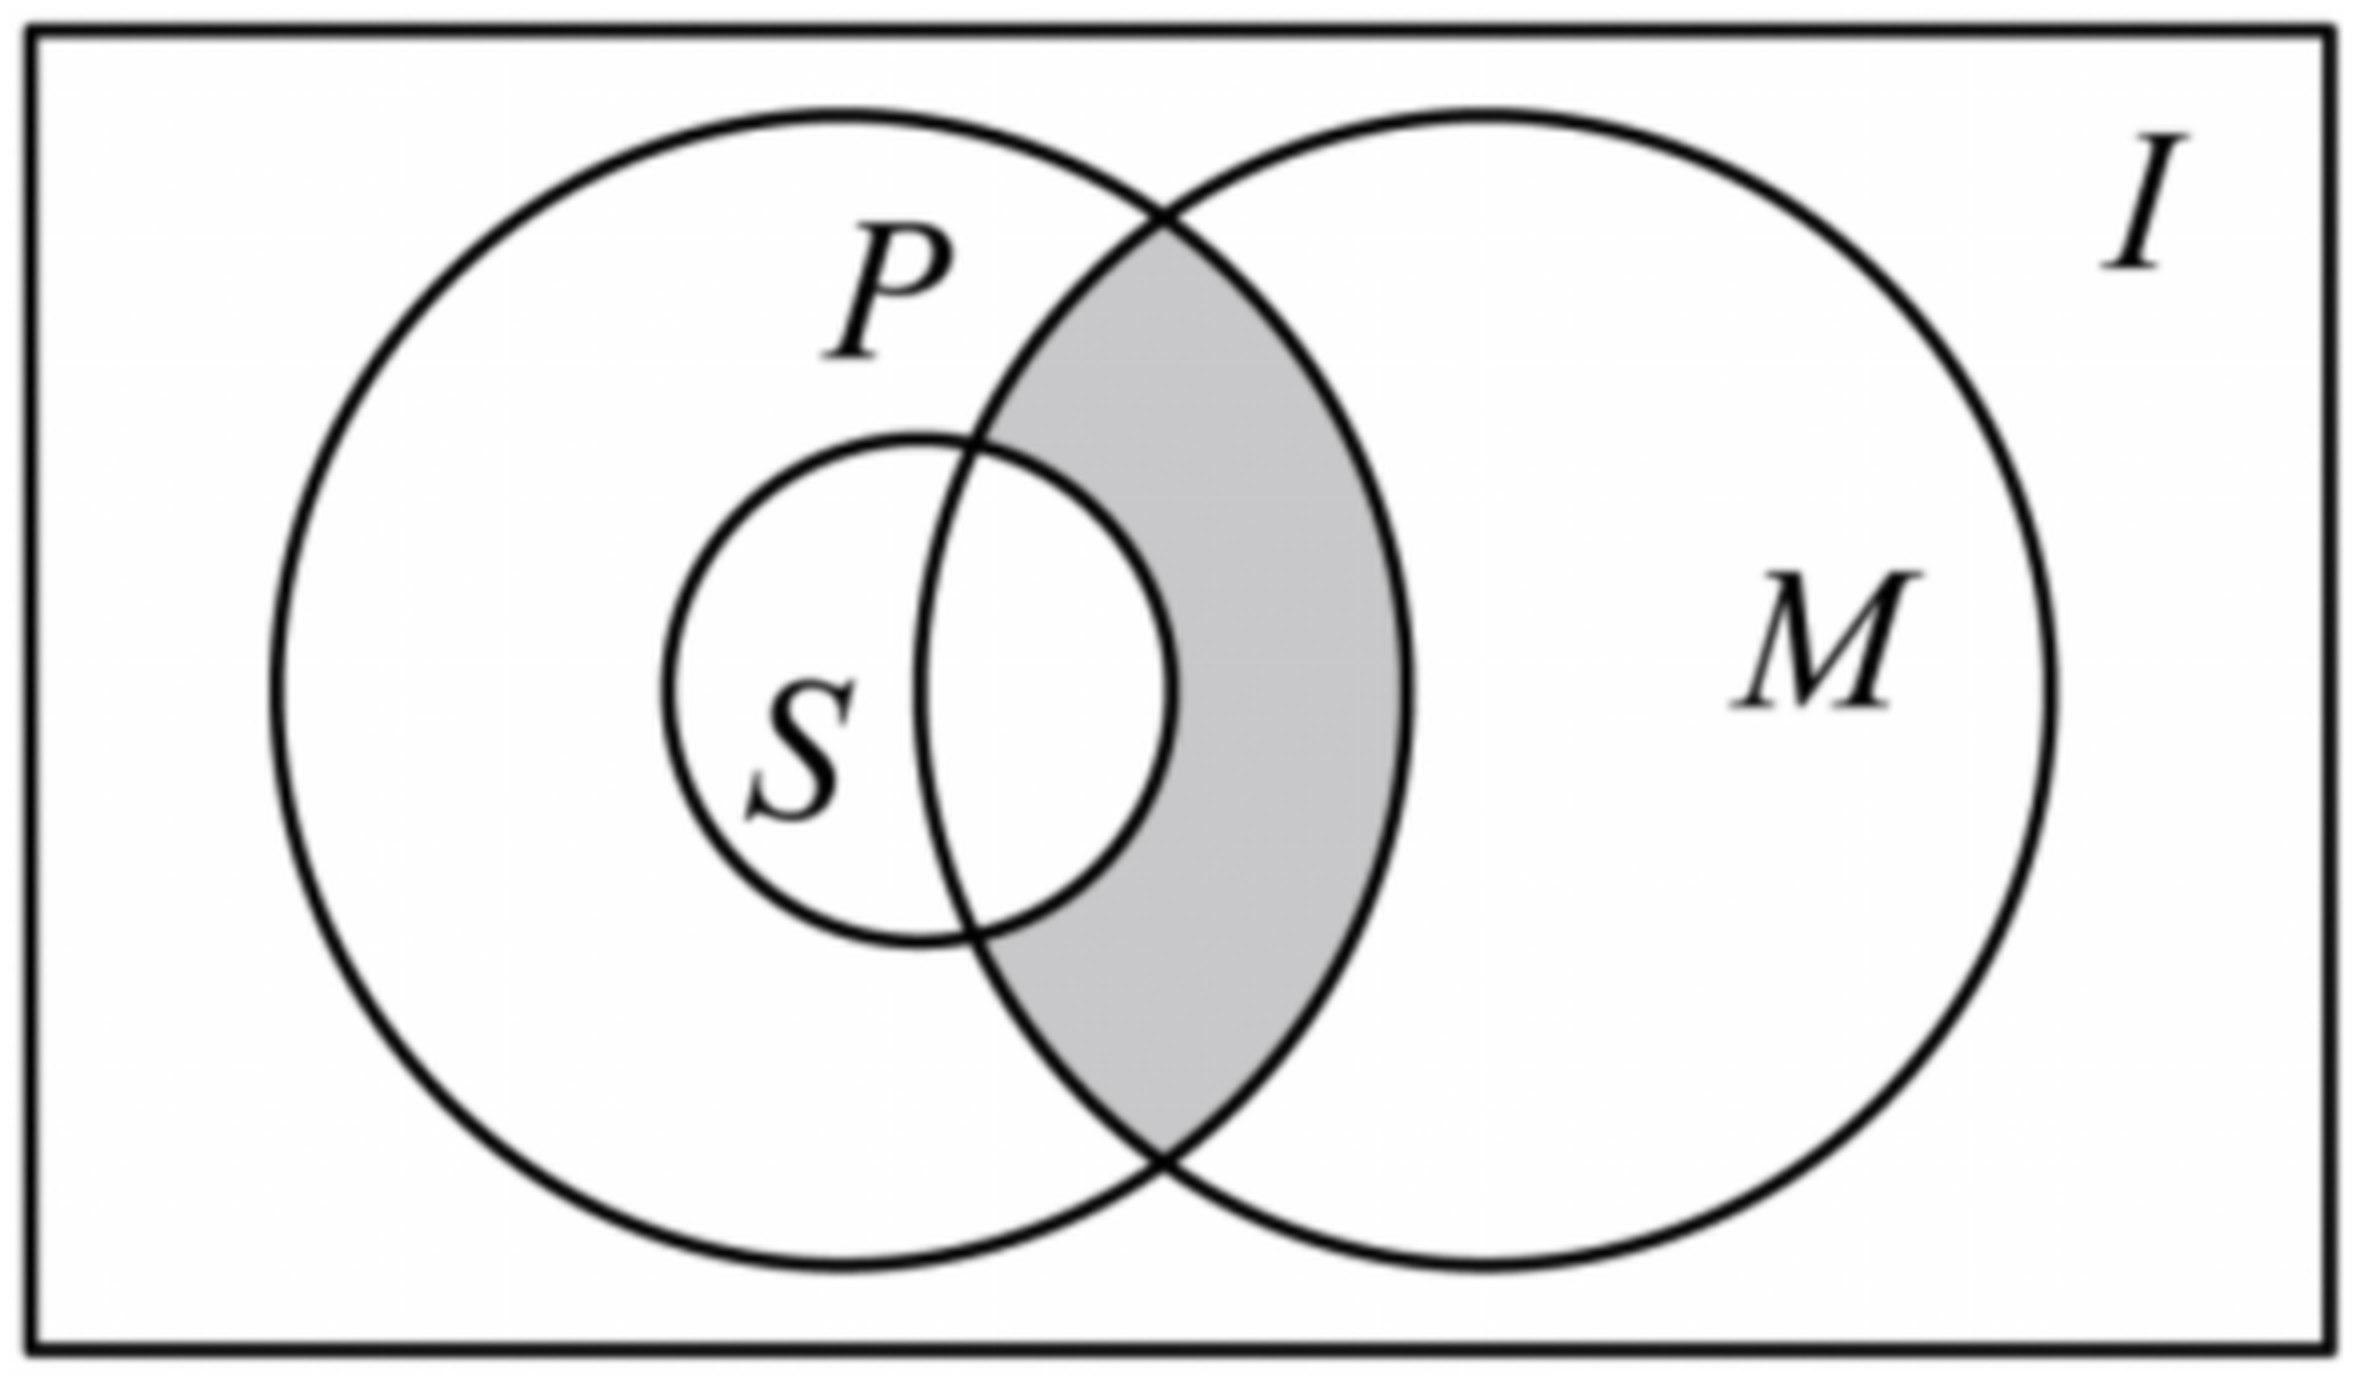
\includegraphics[width=0.46\textwidth]{figures/venn_MP_minus_S_h32.png}
\end{center}

\keepwithprev
A. $(M\cap P)\cap S$\qquad\qquad B. $(M\cap P)\cup S$

C. $(M\cap P)\cap\overline{S}$\qquad\qquad D. $(M\cap P)\cup\overline{S}$

\ans{$C$}

\ifanswer
\solbegin
\step{由 Venn 图得，集合表示 $M$、$P$ 的交集与 $S$ 的补集的交集，}
\step{即阴影部分所表示的集合是 $(M\cap P)\cap\overline{S}$. 故选 $C$.}
\solend

\fi

\item 若实数 $a$、$b$ 满足 $ab>0$，$a+2b=6$，则下列结论中错误的是\mbox{（\quad）}

\keepwithprev
A. $ab\leqslant\dfrac92$\qquad\qquad B. $a^2+4b^2\geqslant18$

C. $\dfrac1a+\dfrac2b$ 的最小值为 $\dfrac94$\qquad\qquad
D. $\dfrac{a^2}{a+1}+\dfrac{4b^2}{2b+1}$ 的最小值为 $\dfrac92$

\ans{$C$}

\ifanswer
\solbegin
\step{因为 $ab>0$，所以 $a$、$b$ 同号，又 $a+2b=6$，所以 $a$、$b$ 同正.}
\step{对于 $A$，由 $6=a+2b\geqslant2\sqrt{a\cdot2b}$ 得 $ab\leqslant\dfrac92$，故 $A$ 正确；}
\step{对于 $B$，由不等式 $\sqrt{\dfrac{m^2+n^2}2}\geqslant\dfrac{m+n}2$ 得
$\sqrt{\dfrac{a^2+(2b)^2}2}\geqslant\dfrac{a+2b}2=3$，}
\step{所以 $a^2+4b^2\geqslant18$，当且仅当 $a=2b=3$ 时取等号，故 $B$ 正确；}
\step{对于 $C$，$\dfrac1a+\dfrac2b
=\dfrac16\left(\dfrac1a+\dfrac2b\right)(a+2b)
=\dfrac16\left(5+\dfrac{2b}a+\dfrac{2a}b\right)$}
\step{$=\dfrac56+\dfrac13\left(\dfrac ba+\dfrac ab\right)
\geqslant\dfrac56+\dfrac13\times2\sqrt{\dfrac ba\cdot\dfrac ab}=\dfrac32$，}
\step{当且仅当 $\dfrac ba=\dfrac ab$，即 $a=b=2$ 时取等号，故 $C$ 错误；}
\step{对于 $D$，$\dfrac{a^2}{a+1}+\dfrac{4b^2}{2b+1}
=\dfrac{(a+1)^2-2(a+1)+1}{a+1}+\dfrac{(2b+1)^2-2(2b+1)+1}{2b+1}$}
\step{$=(a+1)-2+\dfrac1{a+1}+(2b+1)-2+\dfrac1{2b+1}
=(a+2b-2)+\dfrac1{a+1}+\dfrac1{2b+1}$}
\step{$=(6-2)+\dfrac{a+2b+2}{(a+1)(2b+1)}
=4+\dfrac8{(a+1)(2b+1)}$，}
\step{因为 $(a+1)(2b+1)\leqslant\left(\dfrac{a+1+2b+1}2\right)^2
=\left(\dfrac82\right)^2=16$，}
\step{当且仅当 $a+1=2b+1$，即 $a=2b=3$ 时取等号，}
\step{所以 $4+\dfrac8{(a+1)(2b+1)}\geqslant4+\dfrac8{16}=\dfrac92$，
故 $D$ 正确，其他几种方法同 12 题.}
\step{故选 $C$.}
\solend

\fi

% 注：本题的答案「D」原卷直接印在题干末尾的括号内，本稿按全稿惯例另提为 \ans{}。
\item 已知函数 $f(x)=x^2-2ax+a^2-1$，定义集合 $A=\{x\mid f(x)<0\}$. 若集合
$\{x\mid f(x)\in A\}=\varnothing$，则实数 $a$ 的取值范围是\mbox{（\quad）}

\keepwithprev
A. $(-3,-2)$\qquad B. $[-3,-2]$\qquad
C. $(-\infty,2)$\qquad D. $(-\infty,-2]$

\ans{$D$}

\item 非空集合 $A$ 具有如下性质：①若 $x$、$y\in A$，则 $\dfrac xy\in A$；
②若 $x$、$y\in A$，则 $x+y\in A$；

由此可知：下列判断中，错误的是\mbox{（\quad）}

\keepwithprev
A. $-1\notin A$\qquad\qquad B. $\dfrac{2025}{2026}\in A$

C. 若 $x$、$y\in A$，则 $xy\in A$\qquad\qquad
D. 若 $x$、$y\in A$，则 $x-y\in A$

\ans{$D$}

\ifanswer
\solbegin
\step{由题意得 $0\notin A$，$1\in A$，}
\step{对于 $A$，假设 $-1\in A$，则 $-1+1=0\in A$，矛盾，所以 $-1\notin A$，故 $A$ 正确；}
\step{对于 $B$，由 $1\in A$，得 $1+1=2\in A$，$2+1=3\in A$，…，$2025\in A$，$2026\in A$，}
\step{所以 $\dfrac{2025}{2026}\in A$，故 $B$ 正确；}
\step{对于 $C$，因为 $1\in A$，$x\in A$，所以 $\dfrac1x\in A$，
又因为 $y\in A$，所以 $\dfrac y{\frac1x}=xy\in A$，}
\step{故 $C$ 正确；}
\step{对于 $D$，因为 $1\in A$，$2\in A$，若 $x=1$，$y=2$，则 $x-y=-1\notin A$，故 $D$ 错误.}
\step{故选 $D$.}
\solend

\fi

\end{enumerate}

\bigsec{三、解答题}

\begin{enumerate}
\setcounter{enumi}{16}

\item 求下列关于实数 $x$ 的不等式的解集.

\begin{enumerate}[label=(\arabic*)]
\item $|2x+1|<5x-1$；
\item $\dfrac{(x-1)(x-3)(x-6)}{(x-2)(x-4)^2(x-5)}\geqslant0$.
\end{enumerate}

\ifanswer
\solbegin
\stepm{(1)}{因为不等式 $|2x+1|<5x-1$ 可化为 $-(5x-1)<2x+1<5x-1$，且 $5x-1>0$，}
\step{解得 $x>\dfrac23$，所以原不等式的解集为 $\left(\dfrac23,+\infty\right)$；}
\stepm{(2)}{不等式 $\dfrac{(x-1)(x-3)(x-6)}{(x-2)(x-4)^2(x-5)}\geqslant0$，}
\step{等价于 $(x-1)(x-3)(x-6)(x-2)(x-5)\geqslant0$，
且 $x-2\neq0$，$x-4\neq0$，$x-5\neq0$，}
\step{由“穿针引线法”，解得 $1\leqslant x<2$ 或 $3\leqslant x<4$ 或 $4<x<5$ 或 $x\geqslant6$，}
\step{所以不等式的解集为 $[1,2)\cup[3,4)\cup(4,5)\cup[6,+\infty)$.}
\solend

\fi

\ansspace[6]

\item 已知集合 $A=\left\{x\left|mx^2-mx+\dfrac{5m}2-6=0\right.\right\}\neq\varnothing$，
集合 $B=\{x\mid1<x<4$ 且 $x\in\Z\}$，$C=\{x\mid ax+3>0\}$；若 $A\cap B=A$.

\begin{enumerate}[label=(\arabic*)]
\item 求 $m$ 的取值范围.
\item 设 $m$ 的取值集合为 $D$，若 $C\cap D=\varnothing$，求 $m$ 的值及其对应 $a$ 的取值范围.
\end{enumerate}

\ans{略}

\ansspace[8]

\item 已知函数 $f(x)=x^2+(m-2)x+2m-1$.

\begin{enumerate}[label=(\arabic*)]
\item 若 $f(x)=0$ 的两根为 $x_1$、$x_2$，且 $|x_1-x_2|=2$，求实数 $m$ 的值；
\item 若函数 $y=f(x)$ 的图像在区间 $(0,1)$ 上与 $x$ 轴只有一个交点，
求实数 $m$ 的取值范围.
\end{enumerate}

\ifanswer
\solbegin
\stepm{(1)}{由题意得 $x_1+x_2=-(m-2)=2-m$，$x_1x_2=2m-1$，}
\step{由 $|x_1-x_2|=\sqrt{(x_1+x_2)^2-4x_1x_2}
=\sqrt{(2-m)^2-4(2m-1)}=2$，}
\step{化简得 $m^2-12m+4=0$，解得 $m=6\pm4\sqrt2$，故 $m=6\pm4\sqrt2$.}
\stepm{(2)}{当 $f(x)=0$ 只有一个根，且此根位于区间 $(0,1)$，}
\step{则 $\begin{cases}0<\dfrac{2-m}2<1\\[4pt]
\Delta=(m-2)^2-4(2m-1)=0\end{cases}$，
解得 $\begin{cases}0<m<2\\ m=6-2\sqrt7\text{ 或 }m=6+2\sqrt7\end{cases}$，}
\step{所以 $m=6-2\sqrt7$；}
\step{当 $f(x)=0$ 有两个根时，有一个根在区间 $(0,1)$ 内，且另一个根位于 $[0,1]$ 之外，}
\step{则 $\begin{cases}f(0)f(1)<0\\ \Delta=(m-2)^2-4(2m-1)>0\end{cases}$，
解得 $\begin{cases}\dfrac12<m<\dfrac23\\[4pt]
m<6-2\sqrt7\text{ 或 }m>6+2\sqrt7\end{cases}$，}
% 注：下一行原卷作「即 $\dfrac12<m<\dfrac32$」，按上一行方程组应为
%     $\dfrac12<m<\dfrac23$（同页最终答案也印证），照录未改，见文件头「原卷存疑」①。
\step{即 $\dfrac12<m<\dfrac32$；}
\step{当 $f(x)=0$ 有两个根位于区间 $[0,1]$ 内，且只有一个根在区间 $(0,1)$ 内，}
\step{则另一个根为 $0$ 时，得 $m=\dfrac12$，此时 $x_1+x_2=\dfrac32$，
解得另一个根 $x_2=\dfrac32>0$，故此种情况不符题意；}
\step{当 $f(x)=0$ 有两个根位于区间 $(0,1]$ 内，且只有一个根在区间 $(0,1)$ 内，}
\step{则另一个根为 $1$ 时，得 $m=\dfrac23$，此时 $x_1+x_2=\dfrac43$，
解得另一个根 $x_2=\dfrac13$，故此种情况符合题意；}
\step{综上所述，$m$ 的取值范围为
$\left(\dfrac12,\dfrac23\right]\cup\{6-2\sqrt7\}$.}
\solend

\fi

\ansspace[8]

\item 设集合 $A=\{a_1,a_2,a_3,a_4\}$，$B=\{b_1,b_2,b_3,b_4\}$，$C=\{2,3,4,6\}$，
新定义：集合 $A$ 中所有含 $k$ 个元素的子集中 $k$ 个元素之和组成的集合为“$k$ 元集和集”，
集合 $A$ 中所有含 $k$ 个元素的子集中最大元素减去剩余所有元素的和组成的集合为“$k$ 元差集”.

\begin{enumerate}[label=(\arabic*)]
\item 若 $A$ 的“$k$ 元集和集”为 $C$，求：集合 $A$.
\item 在 (1) 的条件下，若 $B$ 的“$k$ 元差集”为 $C$，求：所有满足条件的 $A\cap B$ 的真子集
个数之和.
\item 设 $b_1=a_1^2$，$b_2=a_2^2$，$b_3=a_3^2$，$b_4=a_4^2$，若 $A\cap B$ 为 $2$ 元集且
元素之和为 $10$ 且 $A$ 的“$2$ 元集和集”中最大元素不超过 $14$，求：所有满足条件的 $A$ 的
“$3$ 元差集”.
\end{enumerate}

\ifanswer
\solbegin
\stepm{(1)}{若 $A$ 的“$k$ 元集和集”为 $C$，$C=\{2,3,4,6\}$，则集合为 $\{-1,1,2,3\}$；}
\stepm{(2)}{$B$ 集合为 $\{5,3,0,-1\}$ 或 $\{9,3,1,0\}$ 或 $\{6,3,1,-1\}$，}
\step{故所有 $A\cap B$ 的真子集个数之和为 $13$；}
\stepm{(3)}{$b_1=a_1^2$，$b_2=a_2^2$，$b_3=a_3^2$，$b_4=a_4^2$，}
\step{若 $A\cap B$ 为 $2$ 元集且元素之和为 $10$，
且 $A$ 的“$2$ 元集和集”中最大元素不超过 $14$，}
% 注：下一行答案的第二个集合 $\{0,4,5,6\}$ 是 4 元集，而题问的却是「3 元差集」，
%     原卷如此，照录未改，见文件头「原卷存疑」③。
\step{则满足条件的 $A$ 的“$3$ 元差集” $\{1,3,5\}$ 或 $\{0,4,5,6\}$ 或 $\{2,4,5,8\}$.}
\solend

\fi

\ansspace[8]

\item 已知有限集 $X$、$Y$，定义集合 $X-Y=\{x\mid x\in X$ 且 $x\notin Y\}$，
$|X|$ 表示集合 $X$ 元素个数.

\begin{enumerate}[label=(\arabic*)]
\item 若 $X=\{1,2,3,4\}$，$Y=\{3,4,5\}$，写出集合 $X-Y$ 和 $Y-X$，以及
$|(X-Y)\cup(Y-X)|$ 的值；
\item 给定正整数 $n$，集合 $S=\{1,2,\cdots,n\}$，对于实数集的非空有限子集 $A$、$B$，
定义集合 $C=\{x\mid x=a+b,a\in A,b\in B\}$；

①求证：$|A-S|+|B-S|+|S-C|\geqslant1$；

②求 $|(A-S)\cup(S-A)|+|(B-S)\cup(S-B)|+|(C-S)\cup(S-C)|$ 的最小值.
\end{enumerate}

\ifanswer
\solbegin
\stepm{(1)}{由定义直接得 $X-Y=\{1,2\}$，$Y-X=\{5\}$，
$|(X-Y)\cup(Y-X)|=3$.}
% 注：下一句原卷作「显然 $|X|\geqslant0$」（按后文论证疑为 $|S|\geqslant0$），
%     照录未改，见文件头「原卷存疑」②。
\stepm{(2)}{①显然 $|X|\geqslant0$.}
\step{若 $A\cup B$ 中含有一个不在 $S$ 中的元素，则 $|A-S|+|B-S|\geqslant1$，
即 $|A-S|+|B-S|+|S-C|\geqslant1$.}
\step{若 $A\sub S$，且 $B\sub S$，则 $|A-S|=|B-S|=0$；}
\step{此时 $A$ 中最小的元素 $a\geqslant1$，$B$ 中最小的元素 $b\geqslant1$，
所以 $C$ 中最小的元素 $a+b\geqslant2$，所以 $1\notin C$.}
\step{因为 $S=\{1,2,\cdots,n\}$，所以 $|S-C|\geqslant1$，
即 $|A-S|+|B-S|+|S-C|\geqslant1$.}
\step{综上，$|A-S|+|B-S|+|S-C|\geqslant1$.}
\step{②由①得 $|A-S|+|B-S|+|S-C|\geqslant1$.}
\step{所以 $|(A-S)\cup(S-A)|+|(B-S)\cup(S-B)|+|(C-S)\cup(S-C)|$}
\step{$=|A-S|+|S-A|+|B-S|+|S-B|+|C-S|+|S-C|$}
\step{$\geqslant|S-A|+|S-B|+|C-S|+1$.}
\step{若 $A\cap S=\varnothing$，或 $B\cap S=\varnothing$，则 $|S-A|+|S-B|\geqslant n$.}
\step{若 $A\cap S\neq\varnothing$，且 $B\cap S\neq\varnothing$，
设 $A\cap S=\{a_1,a_2,\cdots,a_s\}$，$B\cap S=\{b_1,b_2,\cdots,b_t\}$，}
\step{且 $1\leqslant a_1<a_2<\cdots<a_s\leqslant n$，
$1\leqslant b_1<b_2<\cdots<b_t\leqslant n$，则 $|S-A|=n-s$，$|B-S|=n-t$.}
% 注：原卷的解析到此为止（第 10 页末），②的最小值并未给出，照录未补，
%     见文件头「原卷存疑」④。
\solend

\fi

\ansspace*[10]

\end{enumerate}

\end{document}
"
% 紧凑版：xelatex "\def\iscompact{1}% 高一32_华师大二附中_周末作业4.tex
%   —— 高一上数学「2026-2027 年华师大二附中高一上周末作业 4」（试卷版/答案版）
% 试卷版：xelatex 高一32_华师大二附中_周末作业4.tex
% 答案版：xelatex "\def\isanswer{1}% 高一32_华师大二附中_周末作业4.tex
%   —— 高一上数学「2026-2027 年华师大二附中高一上周末作业 4」（试卷版/答案版）
% 试卷版：xelatex 高一32_华师大二附中_周末作业4.tex
% 答案版：xelatex "\def\isanswer{1}\input{高一32_华师大二附中_周末作业4.tex}"
% 紧凑版：xelatex "\def\iscompact{1}\input{高一32_华师大二附中_周末作业4.tex}"
%
% 原始材料是微信公众号图文（公众号「魔都数学加油站」连载「27学年高一 32」，2026-09-25 发布，
% 原文标题「27学年高一32——2026-2027年上海市华师大二附中高一上周末作业4」），
% 正文为 10 张 PNG 页。**同一篇里各页分辨率不一致**（2560×3620 与 4762×6735 两档混排），
% 取 mmbiz.qpic.cn/<hash>/0 的原图档。原文本身就是一份**讲评版**——有的题下方印【解析】、
% 有的印【答案】，第 15 题的答案直接印在题干末尾的括号里。
% 试题文字、答案与解析均照原卷录入，未改内容。卷面的粉色斜水印属水印，未录入。
%
% ⚠ 卷首年份：本卷卷面印作「**2025-2026 年**」，与连载「27学年高一32」及公众号原文标题的
%   「2026-2027 年」**不一致**。经三人次分别把标题行裁出放大（4×—10×）独立判读，三次都读作
%   2025-2026，且校名作「华师大二附中」（无「东」字）、卷面亦无「上海市」三字。
%   按全稿「标题行照原卷」的口径，本稿照卷面排作「2025--2026 年…」——这是全稿唯一一份
%   年份不是 2026--2027 的卷子（其余 35 份均为 2026--2027）。
%
% 卷首标题：原卷印作「……年华师大二附中高一上周末作业 4」（公众号标题里的「上海市」
% 三字卷面标题行没有，本稿照卷面），年份区间按全稿惯例排 en dash，前缀照原卷保留「年」。
%
% 与原卷的排版差异（均已在 README「说明」中交代）：
%   ① 原文自**第 3 题**起（第 1、2 题未在该文中发布），故本稿题号亦自 3 起；
%   ② 原卷本就印有「一、填空题」「二、选择题」「三、解答题」三节标题，本稿照原卷分节，
%      只把标题改排成全稿统一的「大节标题」样式；
%   ③ 原卷第 6、8、9 题只印【答案】行（第 18 题的【答案】印作「略”），其余各题印【解析】，
%      第 15 题的答案直接印在题干末尾的括号内；本稿统一改为试卷版隐去、
%      答案版以 \ans{}／\ifanswer 块给出，两版彻底分离；
%   ④ 子集符号原卷两种并用：第 21(2)① 的 $A\sub S$、$B\sub S$ 带下划线，
%      第 3、10 题的 $(0,2)\subset(-\infty,3)$、$A\subset B$、$\overline{B}\subset\overline{A}$
%      作真包含，本稿分别照录为 $\sub$ 与 $\subset$；
%   ⑤ 补集符号原卷一律作上横线（$\overline{A}$、$\overline{B}$、$\overline{S}$），本稿照录；
%      空集原卷作「斜杠伸出圆外」的 $\varnothing$；
%   ⑥ 判别式记号原卷两种：第 4 题作粗体的 $\Delta$、第 11 题作细等宽的 $\triangle$，本稿照录；
%   ⑦ 数集记号原卷作斜体的 $R$、$Z$（第 4、18 题），本稿按全稿惯例统一写作 $\R$、$\Z$；
%   ⑧ 原卷填空的横线约两个字宽，本稿按全稿惯例统一排 \blankline[4.4em]；
%   ⑨ 原卷未印副标题，本稿按全稿惯例补出副标题「集合与常用逻辑用语」；
%   ⑩ 本卷只有第 13 题一图（韦恩图），原卷印在题干右侧，本稿移至题干之后；
%      图取原卷截图、4× LANCZOS 放大（figures/venn_MP_minus_S_h32.png）。
%
% 原卷存疑四处（均照抄原卷、未改，见源码中该处上方注释）：
%   ① 第 19(2)【解析】有「即 $\dfrac12<m<\dfrac32$」，按上一行的方程组应为
%      $\dfrac12<m<\dfrac23$（同页最终答案 $\left(\dfrac12,\dfrac23\right]$ 也印证）；
%   ② 第 21(2)① 首句作「显然 $|X|\geqslant0$」（按后文论证疑为 $|S|\geqslant0$）；
%   ③ 第 20(3) 的答案第二个集合 $\{0,4,5,6\}$ 是 4 元集，而题问的是「3 元差集」；
%   ④ 第 21(2)② 的解析**原卷就未写完**（第 10 页到「则 $|S-A|=n-s$，$|B-S|=n-t$」即止）。

\documentclass[a4paper,11pt]{article}
\usepackage{common}

\begin{document}

\examtitlest[3]{2025--2026 年华师大二附中高一上周末作业 4}{集合与常用逻辑用语}

\bigsec{一、填空题}

\begin{enumerate}
\setcounter{enumi}{2}

\item 设 $x$ 为实数，则“$x<3$”是“$x(x-2)<0$”的 \blankline[4.4em] 条件.

\ifanswer
\solbegin
\step{$x(x-2)<0$，解得 $0<x<2$，$(0,2)\subset(-\infty,3)$，}
\step{若 $x$ 属于“$x(x-2)<0$”，则属于“$x<3$”一定成立，即满足必要性，}
\step{若 $x$ 属于“$x<3$”，不一定满足“$x(x-2)<0$”，如 $x=-1$，即充分性不成立；}
\step{故“$x<3$”是“$x(x-2)<0$”的必要不充分条件.}
\solend

\fi

\item 若关于 $x$ 的不等式 $kx^2-kx+1>0$ 的解集为 $\R$，则实数 $k$ 的取值范围为
\blankline[4.4em].

\ifanswer
\solbegin
\step{①当 $k=0$ 时，不等式为 $1>0$ 恒成立，满足题意；}
\step{②当 $k\neq0$ 时，只要 $\begin{cases}k>0\\ \Delta=k^2-4k<0\end{cases}$，
解得 $0<k<4$；}
\step{所以不等式 $kx^2-kx+1>0$ 的解集为 $\R$，则实数 $k$ 的取值范围为 $[0,4)$.}
\solend

\fi

\item 已知 $1<a<3$，$-5<b<-2$，则 $\dfrac ab$ 的取值范围是 \blankline[4.4em].

\ifanswer
\solbegin
\step{因为 $-5<b<-2$，所以 $2<-b<5$，$\dfrac15<-\dfrac1b<\dfrac12$，又 $1<a<3$，}
\step{得 $\dfrac15<-\dfrac ab<\dfrac32$，则 $-\dfrac32<\dfrac ab<-\dfrac15$，
故 $\dfrac ab$ 的取值范围是 $\left(-\dfrac32,-\dfrac15\right)$.}
\solend

\fi

\item 关于 $x$ 的不等式 $\dfrac{ax-1}{x-a}>1$ 的解集为 $A$，且 $3\notin A$，
则实数 $a$ 的取值范围为 \blankline[4.4em].

\ans{$(-\infty,1]\cup[3,+\infty)$}

\item 若关于 $x$ 的不等式 $a\leqslant\dfrac34x^2-3x+4\leqslant b$ 的解集恰好是 $[a,b]$，
则 $b-a=$ \blankline[4.4em].

\ifanswer
\solbegin
\step{令 $f(x)=\dfrac34x^2-3x+4$，则 $f(x)$ 的对称轴为 $x=2$，}
\step{画出函数 $f(x)=\dfrac34x^2-3x+4=\dfrac34(x-2)^2+1$ 的图象，
得 $f(x)_{\min}=f(2)=1$，}
\step{由题意得 $a\leqslant1$，且 $f(a)=f(b)=b$，$a<b$，}
\step{由 $f(b)=b$ 得 $\dfrac34b^2-3b+4=b$，解得 $b=\dfrac43$（舍去）或 $b=4$，得 $b=4$，}
\step{由抛物线的对称轴为 $x=2$ 得 $a=0$，所以 $b-a=4$.}
\solend

\fi

\item 若关于 $x$ 的方程 $x^2-2kx+k+4=0$ 在 $[1,2]$ 上有解，则实数 $k$ 的取值范围为
\blankline[4.4em].

\ans{$\left[\dfrac83,5\right]$}

\item 记关于 $x$ 的方程 $x^2-2mx-2m+3=0$ 的两实根为 $x_1$、$x_2$，
则 $(x_1-2)^2+(x_2-2)^2$ 的最小值为 \blankline[4.4em].

\ans{$2$}

\item 若“$|mx^2-4x+3|\geqslant2$”的必要非充分条件是“$x\leqslant1$ 或 $x\geqslant4$”，
则实数 $m$ 的取值范围是 \blankline[4.4em].

\ifanswer
\solbegin
\step{记 $|mx^2-4x+3|\geqslant2$ 的解集为集合 $A$，
$B=\{x\mid x\leqslant1\text{ 或 }x\geqslant4\}$，}
\step{则 $\overline{A}$ 为 $|mx^2-4x+3|<2$ 的解集，$\overline{B}=\{x\mid1<x<4\}$；}
\step{因为 $B$ 是 $A$ 的必要非充分条件，所以 $A\subset B$，
得 $\overline{B}\subset\overline{A}$，}
\step{即对任意 $x\in(1,4)$，都有 $|mx^2-4x+3|<2$ 恒成立.}
\step{因为 $|mx^2-4x+3|<2$，$1<x<4$，所以 $-2<mx^2-4x+3<2$，}
\step{化简得
$-5\left(\dfrac1x\right)^2+4\left(\dfrac1x\right)
<m<-\left(\dfrac1x\right)^2+4\left(\dfrac1x\right)$；}
\step{令 $t=\dfrac1x$，$g(t)=-5t^2+4t$，$h(t)=-t^2+4t$，
且 $t\in\left(\dfrac14,1\right)$；}
\step{所以 $g(t)=-5t^2+4t=-5\left(t-\dfrac25\right)^2+\dfrac45$，
当 $t=\dfrac25$ 时，$g(t)$ 取得最大值 $\dfrac45$，}
\step{$h(t)=-t^2+4t=-(t-2)^2+4$，当 $t=\dfrac14$ 时，$h(t)$ 取得最小值，
即 $h(t)>h\left(\dfrac14\right)=\dfrac{15}{16}$；}
\step{因为对任意 $t\in\left(\dfrac14,1\right)$，$g(t)<m<h(t)$ 恒成立，
所以 $g\left(\dfrac25\right)<m\leqslant h\left(\dfrac14\right)$，}
\step{即 $\dfrac45<m\leqslant\dfrac{15}{16}$，
所以 $m$ 的取值范围是 $\left(\dfrac45,\dfrac{15}{16}\right]$.}
\solend

\fi

\item 已知关于 $x$ 的方程 $x^2+2(m-2)x+m^2-3m+3=0$ 有两个不相等的实数根 $x_1$、$x_2$，则

$\dfrac{mx_1}{x_1-1}+\dfrac{mx_2}{x_2-1}-\dfrac2{x_1+x_2-2}$ 的最大值为 \blankline[4.4em].

\ifanswer
\solbegin
\step{关于 $x$ 的方程 $x^2+2(m-2)x+m^2-3m+3=0$ 有两个不相等的实数根 $x_1$、$x_2$，}
\step{则 $\triangle=4(m-2)^2-4(m^2-3m+3)=-4m+4>0$，得 $m<1$，}
\step{且 $x_1+x_2=-2(m-2)$，$x_1x_2=m^2-3m+3$，}
\step{$\dfrac{mx_1}{x_1-1}+\dfrac{mx_2}{x_2-1}-\dfrac2{x_1+x_2-2}
=\dfrac{m[2x_1x_2-(x_1+x_2)]}{x_1x_2-(x_1+x_2)+1}+\dfrac1{m-1}$}
\step{$=\dfrac{2m(m-1)^2}{m^2-m}+\dfrac1{m-1}=2(m-1)+\dfrac1{m-1}$，}
\step{又因为 $m<1$，所以 $m-1<0$，则 $1-m>0$，}
\step{所以 $2(1-m)+\dfrac1{1-m}\geqslant2\sqrt{2(1-m)\cdot\dfrac1{1-m}}=2\sqrt2$，}
\step{当且仅当 $2(1-m)=\dfrac1{1-m}$ 时，即 $m=1-\dfrac{\sqrt2}2$ 时取等号，}
\step{所以 $2(m-1)+\dfrac1{m-1}\leqslant-2\sqrt2$，
即 $\dfrac{mx_1}{x_1-1}+\dfrac{mx_2}{x_2-1}-\dfrac2{x_1+x_2-2}$ 的最大值为 $-2\sqrt2$.}
\solend

\fi

\item 若正实数 $a$、$b$ 满足 $a+2b=ab$，则 $\dfrac4{a^2+2a}+\dfrac1{2b^2+b}$ 的最小值是
\blankline[4.4em].

\ifanswer
\solbegin
\stepm{法一}{由 $a+2b=ab$，得 $\dfrac2a+\dfrac1b=1$，}
\step{令 $x=\dfrac1a$，$y=\dfrac1b$，则 $x$、$y>0$，$2x+y=1$，$2x+1+y+2=4$，}
\step{所以 $\dfrac4{a^2+2a}+\dfrac1{2b^2+b}
=\dfrac4{\frac1{x^2}+\frac2x}+\dfrac1{\frac2{y^2}+\frac1y}
=\dfrac{4x^2}{2x+1}+\dfrac{y^2}{y+2}$（*）}
\step{$=\dfrac{(2x+1)^2-2(2x+1)+1}{2x+1}+\dfrac{(y+2)^2-4(y+2)+4}{y+2}$}
\step{$=2x-1+\dfrac1{2x+1}+y-2+\dfrac4{y+2}=\dfrac1{2x+1}+\dfrac4{y+2}-2$}
\step{$=\dfrac14\left(\dfrac1{2x+1}+\dfrac4{y+2}\right)(2x+1+y+2)-2$}
\step{$=\dfrac14\left[5+\dfrac{y+2}{2x+1}+\dfrac{4(2x+1)}{y+2}\right]-2
\geqslant\dfrac14(5+2\sqrt4)-2=\dfrac14$，}
\step{当且仅当 $\dfrac{y+2}{2x+1}=\dfrac{4(2x+1)}{y+2}$，
即 $x=\dfrac16$，$y=\dfrac23$ 时取等号，}
\step{故 $\dfrac4{a^2+2a}+\dfrac1{2b^2+b}$ 的最小值是 $\dfrac14$.}
\stepm{法二}{在法一（*）后，由权方和不等式，得
$\dfrac4{a^2+2a}+\dfrac1{2b^2+b}
=\dfrac{4x^2}{2x+1}+\dfrac{y^2}{y+2}
\geqslant\dfrac{(2x+y)^2}{2x+1+y+2}=\dfrac14$，}
\step{当且仅当……，故 $\dfrac4{a^2+2a}+\dfrac1{2b^2+b}$ 的最小值是 $\dfrac14$.}
\stepm{法三}{注意到
$\left(\dfrac{a+2}a+\dfrac{2b+1}b\right)\left(\dfrac4{a^2+2a}+\dfrac1{2b^2+b}\right)$}
\step{$\geqslant
\left(\sqrt{\dfrac{a+2}a\cdot\dfrac4{a^2+2a}}
+\sqrt{\dfrac{2b+1}b\cdot\dfrac1{2b^2+b}}\right)^2
=\left(\dfrac2a+\dfrac1b\right)^2$，}
\step{其中 $\dfrac{a+2}a+\dfrac{2b+1}b=3+\dfrac{a+2b}{ab}=4$，
$\dfrac2a+\dfrac1b=\dfrac{a+2b}{ab}=1$，}
\step{所以 $\dfrac4{a^2+2a}+\dfrac1{2b^2+b}\geqslant\dfrac14$，
当且仅当……，故 $\dfrac4{a^2+2a}+\dfrac1{2b^2+b}$ 的最小值是 $\dfrac14$.}
\solend

\fi

\end{enumerate}

\bigsec{二、选择题}

\begin{enumerate}
\setcounter{enumi}{12}

\item 如图，$I$ 为全集，$M$、$P$、$S$ 是 $I$ 的三个子集，则阴影部分所表示的集合是
\mbox{（\quad）}

\begin{center}
% 图取原卷截图、4× LANCZOS 放大（原卷把图印在题干右侧，本稿移至此处，见文件头⑩）。
% 矩形为全集 $I$，左大圆 $P$（内下方含小圆 $S$，其右侧伸入 $P$ 与 $M$ 的重叠区）、
% 右大圆 $M$；阴影是 $P$、$M$ 重叠的透镜形区域挖掉 $S$ 后剩下的部分（左缘呈弯月形）。
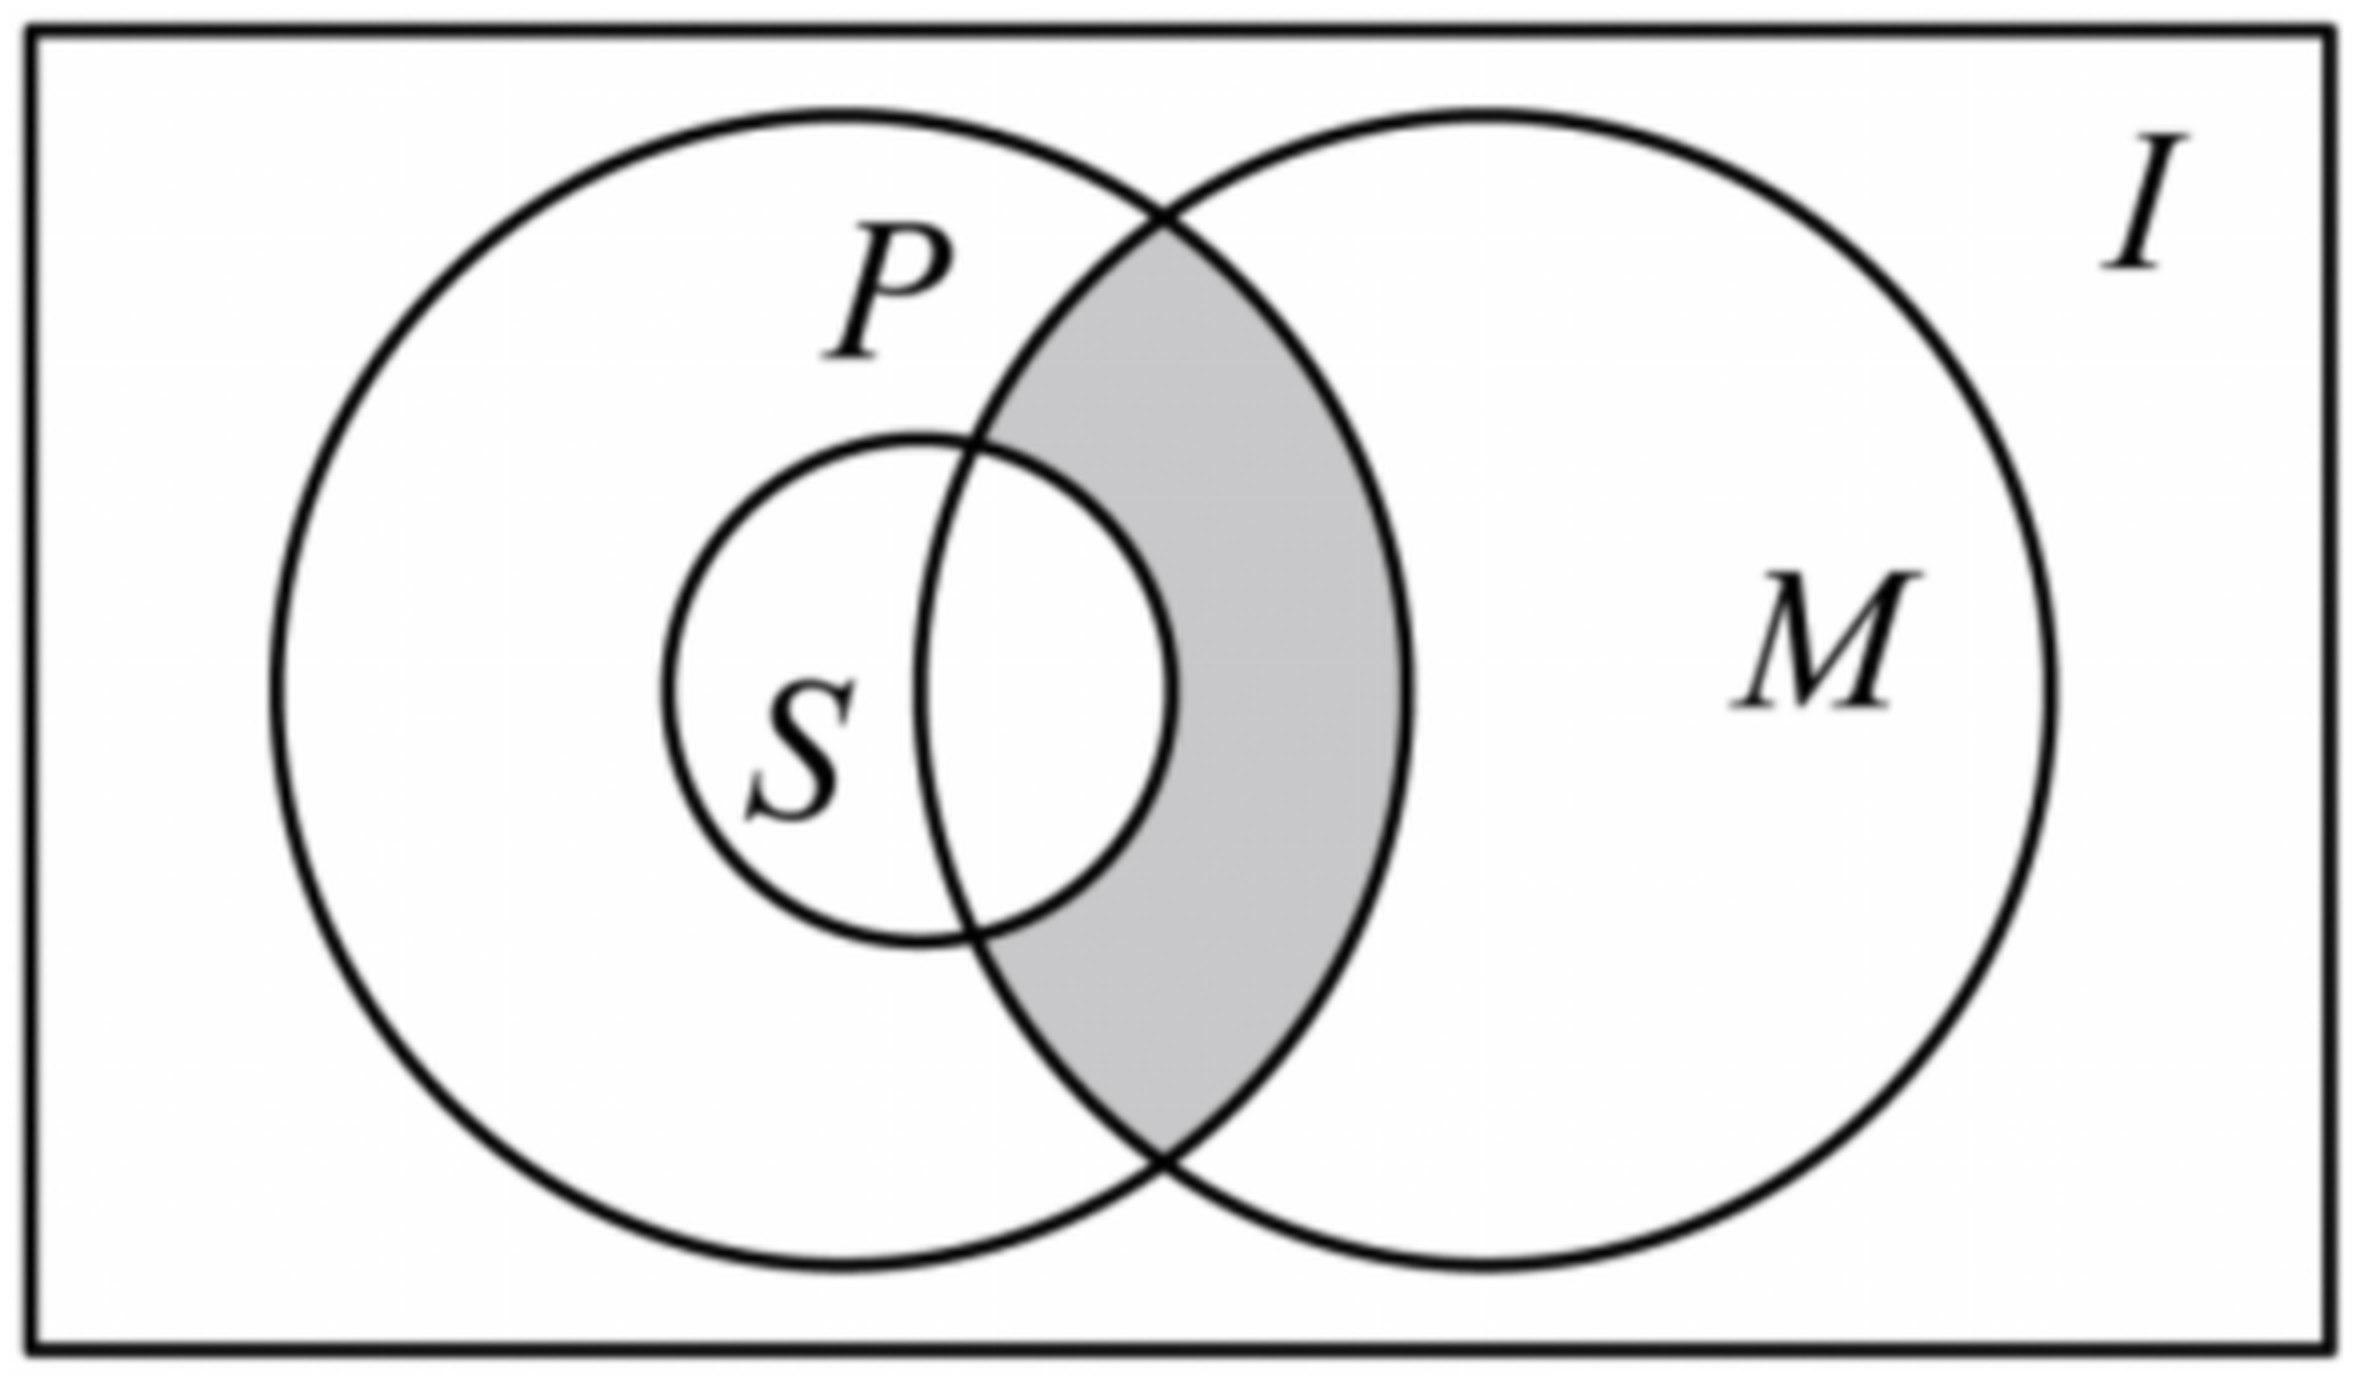
\includegraphics[width=0.46\textwidth]{figures/venn_MP_minus_S_h32.png}
\end{center}

\keepwithprev
A. $(M\cap P)\cap S$\qquad\qquad B. $(M\cap P)\cup S$

C. $(M\cap P)\cap\overline{S}$\qquad\qquad D. $(M\cap P)\cup\overline{S}$

\ans{$C$}

\ifanswer
\solbegin
\step{由 Venn 图得，集合表示 $M$、$P$ 的交集与 $S$ 的补集的交集，}
\step{即阴影部分所表示的集合是 $(M\cap P)\cap\overline{S}$. 故选 $C$.}
\solend

\fi

\item 若实数 $a$、$b$ 满足 $ab>0$，$a+2b=6$，则下列结论中错误的是\mbox{（\quad）}

\keepwithprev
A. $ab\leqslant\dfrac92$\qquad\qquad B. $a^2+4b^2\geqslant18$

C. $\dfrac1a+\dfrac2b$ 的最小值为 $\dfrac94$\qquad\qquad
D. $\dfrac{a^2}{a+1}+\dfrac{4b^2}{2b+1}$ 的最小值为 $\dfrac92$

\ans{$C$}

\ifanswer
\solbegin
\step{因为 $ab>0$，所以 $a$、$b$ 同号，又 $a+2b=6$，所以 $a$、$b$ 同正.}
\step{对于 $A$，由 $6=a+2b\geqslant2\sqrt{a\cdot2b}$ 得 $ab\leqslant\dfrac92$，故 $A$ 正确；}
\step{对于 $B$，由不等式 $\sqrt{\dfrac{m^2+n^2}2}\geqslant\dfrac{m+n}2$ 得
$\sqrt{\dfrac{a^2+(2b)^2}2}\geqslant\dfrac{a+2b}2=3$，}
\step{所以 $a^2+4b^2\geqslant18$，当且仅当 $a=2b=3$ 时取等号，故 $B$ 正确；}
\step{对于 $C$，$\dfrac1a+\dfrac2b
=\dfrac16\left(\dfrac1a+\dfrac2b\right)(a+2b)
=\dfrac16\left(5+\dfrac{2b}a+\dfrac{2a}b\right)$}
\step{$=\dfrac56+\dfrac13\left(\dfrac ba+\dfrac ab\right)
\geqslant\dfrac56+\dfrac13\times2\sqrt{\dfrac ba\cdot\dfrac ab}=\dfrac32$，}
\step{当且仅当 $\dfrac ba=\dfrac ab$，即 $a=b=2$ 时取等号，故 $C$ 错误；}
\step{对于 $D$，$\dfrac{a^2}{a+1}+\dfrac{4b^2}{2b+1}
=\dfrac{(a+1)^2-2(a+1)+1}{a+1}+\dfrac{(2b+1)^2-2(2b+1)+1}{2b+1}$}
\step{$=(a+1)-2+\dfrac1{a+1}+(2b+1)-2+\dfrac1{2b+1}
=(a+2b-2)+\dfrac1{a+1}+\dfrac1{2b+1}$}
\step{$=(6-2)+\dfrac{a+2b+2}{(a+1)(2b+1)}
=4+\dfrac8{(a+1)(2b+1)}$，}
\step{因为 $(a+1)(2b+1)\leqslant\left(\dfrac{a+1+2b+1}2\right)^2
=\left(\dfrac82\right)^2=16$，}
\step{当且仅当 $a+1=2b+1$，即 $a=2b=3$ 时取等号，}
\step{所以 $4+\dfrac8{(a+1)(2b+1)}\geqslant4+\dfrac8{16}=\dfrac92$，
故 $D$ 正确，其他几种方法同 12 题.}
\step{故选 $C$.}
\solend

\fi

% 注：本题的答案「D」原卷直接印在题干末尾的括号内，本稿按全稿惯例另提为 \ans{}。
\item 已知函数 $f(x)=x^2-2ax+a^2-1$，定义集合 $A=\{x\mid f(x)<0\}$. 若集合
$\{x\mid f(x)\in A\}=\varnothing$，则实数 $a$ 的取值范围是\mbox{（\quad）}

\keepwithprev
A. $(-3,-2)$\qquad B. $[-3,-2]$\qquad
C. $(-\infty,2)$\qquad D. $(-\infty,-2]$

\ans{$D$}

\item 非空集合 $A$ 具有如下性质：①若 $x$、$y\in A$，则 $\dfrac xy\in A$；
②若 $x$、$y\in A$，则 $x+y\in A$；

由此可知：下列判断中，错误的是\mbox{（\quad）}

\keepwithprev
A. $-1\notin A$\qquad\qquad B. $\dfrac{2025}{2026}\in A$

C. 若 $x$、$y\in A$，则 $xy\in A$\qquad\qquad
D. 若 $x$、$y\in A$，则 $x-y\in A$

\ans{$D$}

\ifanswer
\solbegin
\step{由题意得 $0\notin A$，$1\in A$，}
\step{对于 $A$，假设 $-1\in A$，则 $-1+1=0\in A$，矛盾，所以 $-1\notin A$，故 $A$ 正确；}
\step{对于 $B$，由 $1\in A$，得 $1+1=2\in A$，$2+1=3\in A$，…，$2025\in A$，$2026\in A$，}
\step{所以 $\dfrac{2025}{2026}\in A$，故 $B$ 正确；}
\step{对于 $C$，因为 $1\in A$，$x\in A$，所以 $\dfrac1x\in A$，
又因为 $y\in A$，所以 $\dfrac y{\frac1x}=xy\in A$，}
\step{故 $C$ 正确；}
\step{对于 $D$，因为 $1\in A$，$2\in A$，若 $x=1$，$y=2$，则 $x-y=-1\notin A$，故 $D$ 错误.}
\step{故选 $D$.}
\solend

\fi

\end{enumerate}

\bigsec{三、解答题}

\begin{enumerate}
\setcounter{enumi}{16}

\item 求下列关于实数 $x$ 的不等式的解集.

\begin{enumerate}[label=(\arabic*)]
\item $|2x+1|<5x-1$；
\item $\dfrac{(x-1)(x-3)(x-6)}{(x-2)(x-4)^2(x-5)}\geqslant0$.
\end{enumerate}

\ifanswer
\solbegin
\stepm{(1)}{因为不等式 $|2x+1|<5x-1$ 可化为 $-(5x-1)<2x+1<5x-1$，且 $5x-1>0$，}
\step{解得 $x>\dfrac23$，所以原不等式的解集为 $\left(\dfrac23,+\infty\right)$；}
\stepm{(2)}{不等式 $\dfrac{(x-1)(x-3)(x-6)}{(x-2)(x-4)^2(x-5)}\geqslant0$，}
\step{等价于 $(x-1)(x-3)(x-6)(x-2)(x-5)\geqslant0$，
且 $x-2\neq0$，$x-4\neq0$，$x-5\neq0$，}
\step{由“穿针引线法”，解得 $1\leqslant x<2$ 或 $3\leqslant x<4$ 或 $4<x<5$ 或 $x\geqslant6$，}
\step{所以不等式的解集为 $[1,2)\cup[3,4)\cup(4,5)\cup[6,+\infty)$.}
\solend

\fi

\ansspace[6]

\item 已知集合 $A=\left\{x\left|mx^2-mx+\dfrac{5m}2-6=0\right.\right\}\neq\varnothing$，
集合 $B=\{x\mid1<x<4$ 且 $x\in\Z\}$，$C=\{x\mid ax+3>0\}$；若 $A\cap B=A$.

\begin{enumerate}[label=(\arabic*)]
\item 求 $m$ 的取值范围.
\item 设 $m$ 的取值集合为 $D$，若 $C\cap D=\varnothing$，求 $m$ 的值及其对应 $a$ 的取值范围.
\end{enumerate}

\ans{略}

\ansspace[8]

\item 已知函数 $f(x)=x^2+(m-2)x+2m-1$.

\begin{enumerate}[label=(\arabic*)]
\item 若 $f(x)=0$ 的两根为 $x_1$、$x_2$，且 $|x_1-x_2|=2$，求实数 $m$ 的值；
\item 若函数 $y=f(x)$ 的图像在区间 $(0,1)$ 上与 $x$ 轴只有一个交点，
求实数 $m$ 的取值范围.
\end{enumerate}

\ifanswer
\solbegin
\stepm{(1)}{由题意得 $x_1+x_2=-(m-2)=2-m$，$x_1x_2=2m-1$，}
\step{由 $|x_1-x_2|=\sqrt{(x_1+x_2)^2-4x_1x_2}
=\sqrt{(2-m)^2-4(2m-1)}=2$，}
\step{化简得 $m^2-12m+4=0$，解得 $m=6\pm4\sqrt2$，故 $m=6\pm4\sqrt2$.}
\stepm{(2)}{当 $f(x)=0$ 只有一个根，且此根位于区间 $(0,1)$，}
\step{则 $\begin{cases}0<\dfrac{2-m}2<1\\[4pt]
\Delta=(m-2)^2-4(2m-1)=0\end{cases}$，
解得 $\begin{cases}0<m<2\\ m=6-2\sqrt7\text{ 或 }m=6+2\sqrt7\end{cases}$，}
\step{所以 $m=6-2\sqrt7$；}
\step{当 $f(x)=0$ 有两个根时，有一个根在区间 $(0,1)$ 内，且另一个根位于 $[0,1]$ 之外，}
\step{则 $\begin{cases}f(0)f(1)<0\\ \Delta=(m-2)^2-4(2m-1)>0\end{cases}$，
解得 $\begin{cases}\dfrac12<m<\dfrac23\\[4pt]
m<6-2\sqrt7\text{ 或 }m>6+2\sqrt7\end{cases}$，}
% 注：下一行原卷作「即 $\dfrac12<m<\dfrac32$」，按上一行方程组应为
%     $\dfrac12<m<\dfrac23$（同页最终答案也印证），照录未改，见文件头「原卷存疑」①。
\step{即 $\dfrac12<m<\dfrac32$；}
\step{当 $f(x)=0$ 有两个根位于区间 $[0,1]$ 内，且只有一个根在区间 $(0,1)$ 内，}
\step{则另一个根为 $0$ 时，得 $m=\dfrac12$，此时 $x_1+x_2=\dfrac32$，
解得另一个根 $x_2=\dfrac32>0$，故此种情况不符题意；}
\step{当 $f(x)=0$ 有两个根位于区间 $(0,1]$ 内，且只有一个根在区间 $(0,1)$ 内，}
\step{则另一个根为 $1$ 时，得 $m=\dfrac23$，此时 $x_1+x_2=\dfrac43$，
解得另一个根 $x_2=\dfrac13$，故此种情况符合题意；}
\step{综上所述，$m$ 的取值范围为
$\left(\dfrac12,\dfrac23\right]\cup\{6-2\sqrt7\}$.}
\solend

\fi

\ansspace[8]

\item 设集合 $A=\{a_1,a_2,a_3,a_4\}$，$B=\{b_1,b_2,b_3,b_4\}$，$C=\{2,3,4,6\}$，
新定义：集合 $A$ 中所有含 $k$ 个元素的子集中 $k$ 个元素之和组成的集合为“$k$ 元集和集”，
集合 $A$ 中所有含 $k$ 个元素的子集中最大元素减去剩余所有元素的和组成的集合为“$k$ 元差集”.

\begin{enumerate}[label=(\arabic*)]
\item 若 $A$ 的“$k$ 元集和集”为 $C$，求：集合 $A$.
\item 在 (1) 的条件下，若 $B$ 的“$k$ 元差集”为 $C$，求：所有满足条件的 $A\cap B$ 的真子集
个数之和.
\item 设 $b_1=a_1^2$，$b_2=a_2^2$，$b_3=a_3^2$，$b_4=a_4^2$，若 $A\cap B$ 为 $2$ 元集且
元素之和为 $10$ 且 $A$ 的“$2$ 元集和集”中最大元素不超过 $14$，求：所有满足条件的 $A$ 的
“$3$ 元差集”.
\end{enumerate}

\ifanswer
\solbegin
\stepm{(1)}{若 $A$ 的“$k$ 元集和集”为 $C$，$C=\{2,3,4,6\}$，则集合为 $\{-1,1,2,3\}$；}
\stepm{(2)}{$B$ 集合为 $\{5,3,0,-1\}$ 或 $\{9,3,1,0\}$ 或 $\{6,3,1,-1\}$，}
\step{故所有 $A\cap B$ 的真子集个数之和为 $13$；}
\stepm{(3)}{$b_1=a_1^2$，$b_2=a_2^2$，$b_3=a_3^2$，$b_4=a_4^2$，}
\step{若 $A\cap B$ 为 $2$ 元集且元素之和为 $10$，
且 $A$ 的“$2$ 元集和集”中最大元素不超过 $14$，}
% 注：下一行答案的第二个集合 $\{0,4,5,6\}$ 是 4 元集，而题问的却是「3 元差集」，
%     原卷如此，照录未改，见文件头「原卷存疑」③。
\step{则满足条件的 $A$ 的“$3$ 元差集” $\{1,3,5\}$ 或 $\{0,4,5,6\}$ 或 $\{2,4,5,8\}$.}
\solend

\fi

\ansspace[8]

\item 已知有限集 $X$、$Y$，定义集合 $X-Y=\{x\mid x\in X$ 且 $x\notin Y\}$，
$|X|$ 表示集合 $X$ 元素个数.

\begin{enumerate}[label=(\arabic*)]
\item 若 $X=\{1,2,3,4\}$，$Y=\{3,4,5\}$，写出集合 $X-Y$ 和 $Y-X$，以及
$|(X-Y)\cup(Y-X)|$ 的值；
\item 给定正整数 $n$，集合 $S=\{1,2,\cdots,n\}$，对于实数集的非空有限子集 $A$、$B$，
定义集合 $C=\{x\mid x=a+b,a\in A,b\in B\}$；

①求证：$|A-S|+|B-S|+|S-C|\geqslant1$；

②求 $|(A-S)\cup(S-A)|+|(B-S)\cup(S-B)|+|(C-S)\cup(S-C)|$ 的最小值.
\end{enumerate}

\ifanswer
\solbegin
\stepm{(1)}{由定义直接得 $X-Y=\{1,2\}$，$Y-X=\{5\}$，
$|(X-Y)\cup(Y-X)|=3$.}
% 注：下一句原卷作「显然 $|X|\geqslant0$」（按后文论证疑为 $|S|\geqslant0$），
%     照录未改，见文件头「原卷存疑」②。
\stepm{(2)}{①显然 $|X|\geqslant0$.}
\step{若 $A\cup B$ 中含有一个不在 $S$ 中的元素，则 $|A-S|+|B-S|\geqslant1$，
即 $|A-S|+|B-S|+|S-C|\geqslant1$.}
\step{若 $A\sub S$，且 $B\sub S$，则 $|A-S|=|B-S|=0$；}
\step{此时 $A$ 中最小的元素 $a\geqslant1$，$B$ 中最小的元素 $b\geqslant1$，
所以 $C$ 中最小的元素 $a+b\geqslant2$，所以 $1\notin C$.}
\step{因为 $S=\{1,2,\cdots,n\}$，所以 $|S-C|\geqslant1$，
即 $|A-S|+|B-S|+|S-C|\geqslant1$.}
\step{综上，$|A-S|+|B-S|+|S-C|\geqslant1$.}
\step{②由①得 $|A-S|+|B-S|+|S-C|\geqslant1$.}
\step{所以 $|(A-S)\cup(S-A)|+|(B-S)\cup(S-B)|+|(C-S)\cup(S-C)|$}
\step{$=|A-S|+|S-A|+|B-S|+|S-B|+|C-S|+|S-C|$}
\step{$\geqslant|S-A|+|S-B|+|C-S|+1$.}
\step{若 $A\cap S=\varnothing$，或 $B\cap S=\varnothing$，则 $|S-A|+|S-B|\geqslant n$.}
\step{若 $A\cap S\neq\varnothing$，且 $B\cap S\neq\varnothing$，
设 $A\cap S=\{a_1,a_2,\cdots,a_s\}$，$B\cap S=\{b_1,b_2,\cdots,b_t\}$，}
\step{且 $1\leqslant a_1<a_2<\cdots<a_s\leqslant n$，
$1\leqslant b_1<b_2<\cdots<b_t\leqslant n$，则 $|S-A|=n-s$，$|B-S|=n-t$.}
% 注：原卷的解析到此为止（第 10 页末），②的最小值并未给出，照录未补，
%     见文件头「原卷存疑」④。
\solend

\fi

\ansspace*[10]

\end{enumerate}

\end{document}
"
% 紧凑版：xelatex "\def\iscompact{1}% 高一32_华师大二附中_周末作业4.tex
%   —— 高一上数学「2026-2027 年华师大二附中高一上周末作业 4」（试卷版/答案版）
% 试卷版：xelatex 高一32_华师大二附中_周末作业4.tex
% 答案版：xelatex "\def\isanswer{1}\input{高一32_华师大二附中_周末作业4.tex}"
% 紧凑版：xelatex "\def\iscompact{1}\input{高一32_华师大二附中_周末作业4.tex}"
%
% 原始材料是微信公众号图文（公众号「魔都数学加油站」连载「27学年高一 32」，2026-09-25 发布，
% 原文标题「27学年高一32——2026-2027年上海市华师大二附中高一上周末作业4」），
% 正文为 10 张 PNG 页。**同一篇里各页分辨率不一致**（2560×3620 与 4762×6735 两档混排），
% 取 mmbiz.qpic.cn/<hash>/0 的原图档。原文本身就是一份**讲评版**——有的题下方印【解析】、
% 有的印【答案】，第 15 题的答案直接印在题干末尾的括号里。
% 试题文字、答案与解析均照原卷录入，未改内容。卷面的粉色斜水印属水印，未录入。
%
% ⚠ 卷首年份：本卷卷面印作「**2025-2026 年**」，与连载「27学年高一32」及公众号原文标题的
%   「2026-2027 年」**不一致**。经三人次分别把标题行裁出放大（4×—10×）独立判读，三次都读作
%   2025-2026，且校名作「华师大二附中」（无「东」字）、卷面亦无「上海市」三字。
%   按全稿「标题行照原卷」的口径，本稿照卷面排作「2025--2026 年…」——这是全稿唯一一份
%   年份不是 2026--2027 的卷子（其余 35 份均为 2026--2027）。
%
% 卷首标题：原卷印作「……年华师大二附中高一上周末作业 4」（公众号标题里的「上海市」
% 三字卷面标题行没有，本稿照卷面），年份区间按全稿惯例排 en dash，前缀照原卷保留「年」。
%
% 与原卷的排版差异（均已在 README「说明」中交代）：
%   ① 原文自**第 3 题**起（第 1、2 题未在该文中发布），故本稿题号亦自 3 起；
%   ② 原卷本就印有「一、填空题」「二、选择题」「三、解答题」三节标题，本稿照原卷分节，
%      只把标题改排成全稿统一的「大节标题」样式；
%   ③ 原卷第 6、8、9 题只印【答案】行（第 18 题的【答案】印作「略”），其余各题印【解析】，
%      第 15 题的答案直接印在题干末尾的括号内；本稿统一改为试卷版隐去、
%      答案版以 \ans{}／\ifanswer 块给出，两版彻底分离；
%   ④ 子集符号原卷两种并用：第 21(2)① 的 $A\sub S$、$B\sub S$ 带下划线，
%      第 3、10 题的 $(0,2)\subset(-\infty,3)$、$A\subset B$、$\overline{B}\subset\overline{A}$
%      作真包含，本稿分别照录为 $\sub$ 与 $\subset$；
%   ⑤ 补集符号原卷一律作上横线（$\overline{A}$、$\overline{B}$、$\overline{S}$），本稿照录；
%      空集原卷作「斜杠伸出圆外」的 $\varnothing$；
%   ⑥ 判别式记号原卷两种：第 4 题作粗体的 $\Delta$、第 11 题作细等宽的 $\triangle$，本稿照录；
%   ⑦ 数集记号原卷作斜体的 $R$、$Z$（第 4、18 题），本稿按全稿惯例统一写作 $\R$、$\Z$；
%   ⑧ 原卷填空的横线约两个字宽，本稿按全稿惯例统一排 \blankline[4.4em]；
%   ⑨ 原卷未印副标题，本稿按全稿惯例补出副标题「集合与常用逻辑用语」；
%   ⑩ 本卷只有第 13 题一图（韦恩图），原卷印在题干右侧，本稿移至题干之后；
%      图取原卷截图、4× LANCZOS 放大（figures/venn_MP_minus_S_h32.png）。
%
% 原卷存疑四处（均照抄原卷、未改，见源码中该处上方注释）：
%   ① 第 19(2)【解析】有「即 $\dfrac12<m<\dfrac32$」，按上一行的方程组应为
%      $\dfrac12<m<\dfrac23$（同页最终答案 $\left(\dfrac12,\dfrac23\right]$ 也印证）；
%   ② 第 21(2)① 首句作「显然 $|X|\geqslant0$」（按后文论证疑为 $|S|\geqslant0$）；
%   ③ 第 20(3) 的答案第二个集合 $\{0,4,5,6\}$ 是 4 元集，而题问的是「3 元差集」；
%   ④ 第 21(2)② 的解析**原卷就未写完**（第 10 页到「则 $|S-A|=n-s$，$|B-S|=n-t$」即止）。

\documentclass[a4paper,11pt]{article}
\usepackage{common}

\begin{document}

\examtitlest[3]{2025--2026 年华师大二附中高一上周末作业 4}{集合与常用逻辑用语}

\bigsec{一、填空题}

\begin{enumerate}
\setcounter{enumi}{2}

\item 设 $x$ 为实数，则“$x<3$”是“$x(x-2)<0$”的 \blankline[4.4em] 条件.

\ifanswer
\solbegin
\step{$x(x-2)<0$，解得 $0<x<2$，$(0,2)\subset(-\infty,3)$，}
\step{若 $x$ 属于“$x(x-2)<0$”，则属于“$x<3$”一定成立，即满足必要性，}
\step{若 $x$ 属于“$x<3$”，不一定满足“$x(x-2)<0$”，如 $x=-1$，即充分性不成立；}
\step{故“$x<3$”是“$x(x-2)<0$”的必要不充分条件.}
\solend

\fi

\item 若关于 $x$ 的不等式 $kx^2-kx+1>0$ 的解集为 $\R$，则实数 $k$ 的取值范围为
\blankline[4.4em].

\ifanswer
\solbegin
\step{①当 $k=0$ 时，不等式为 $1>0$ 恒成立，满足题意；}
\step{②当 $k\neq0$ 时，只要 $\begin{cases}k>0\\ \Delta=k^2-4k<0\end{cases}$，
解得 $0<k<4$；}
\step{所以不等式 $kx^2-kx+1>0$ 的解集为 $\R$，则实数 $k$ 的取值范围为 $[0,4)$.}
\solend

\fi

\item 已知 $1<a<3$，$-5<b<-2$，则 $\dfrac ab$ 的取值范围是 \blankline[4.4em].

\ifanswer
\solbegin
\step{因为 $-5<b<-2$，所以 $2<-b<5$，$\dfrac15<-\dfrac1b<\dfrac12$，又 $1<a<3$，}
\step{得 $\dfrac15<-\dfrac ab<\dfrac32$，则 $-\dfrac32<\dfrac ab<-\dfrac15$，
故 $\dfrac ab$ 的取值范围是 $\left(-\dfrac32,-\dfrac15\right)$.}
\solend

\fi

\item 关于 $x$ 的不等式 $\dfrac{ax-1}{x-a}>1$ 的解集为 $A$，且 $3\notin A$，
则实数 $a$ 的取值范围为 \blankline[4.4em].

\ans{$(-\infty,1]\cup[3,+\infty)$}

\item 若关于 $x$ 的不等式 $a\leqslant\dfrac34x^2-3x+4\leqslant b$ 的解集恰好是 $[a,b]$，
则 $b-a=$ \blankline[4.4em].

\ifanswer
\solbegin
\step{令 $f(x)=\dfrac34x^2-3x+4$，则 $f(x)$ 的对称轴为 $x=2$，}
\step{画出函数 $f(x)=\dfrac34x^2-3x+4=\dfrac34(x-2)^2+1$ 的图象，
得 $f(x)_{\min}=f(2)=1$，}
\step{由题意得 $a\leqslant1$，且 $f(a)=f(b)=b$，$a<b$，}
\step{由 $f(b)=b$ 得 $\dfrac34b^2-3b+4=b$，解得 $b=\dfrac43$（舍去）或 $b=4$，得 $b=4$，}
\step{由抛物线的对称轴为 $x=2$ 得 $a=0$，所以 $b-a=4$.}
\solend

\fi

\item 若关于 $x$ 的方程 $x^2-2kx+k+4=0$ 在 $[1,2]$ 上有解，则实数 $k$ 的取值范围为
\blankline[4.4em].

\ans{$\left[\dfrac83,5\right]$}

\item 记关于 $x$ 的方程 $x^2-2mx-2m+3=0$ 的两实根为 $x_1$、$x_2$，
则 $(x_1-2)^2+(x_2-2)^2$ 的最小值为 \blankline[4.4em].

\ans{$2$}

\item 若“$|mx^2-4x+3|\geqslant2$”的必要非充分条件是“$x\leqslant1$ 或 $x\geqslant4$”，
则实数 $m$ 的取值范围是 \blankline[4.4em].

\ifanswer
\solbegin
\step{记 $|mx^2-4x+3|\geqslant2$ 的解集为集合 $A$，
$B=\{x\mid x\leqslant1\text{ 或 }x\geqslant4\}$，}
\step{则 $\overline{A}$ 为 $|mx^2-4x+3|<2$ 的解集，$\overline{B}=\{x\mid1<x<4\}$；}
\step{因为 $B$ 是 $A$ 的必要非充分条件，所以 $A\subset B$，
得 $\overline{B}\subset\overline{A}$，}
\step{即对任意 $x\in(1,4)$，都有 $|mx^2-4x+3|<2$ 恒成立.}
\step{因为 $|mx^2-4x+3|<2$，$1<x<4$，所以 $-2<mx^2-4x+3<2$，}
\step{化简得
$-5\left(\dfrac1x\right)^2+4\left(\dfrac1x\right)
<m<-\left(\dfrac1x\right)^2+4\left(\dfrac1x\right)$；}
\step{令 $t=\dfrac1x$，$g(t)=-5t^2+4t$，$h(t)=-t^2+4t$，
且 $t\in\left(\dfrac14,1\right)$；}
\step{所以 $g(t)=-5t^2+4t=-5\left(t-\dfrac25\right)^2+\dfrac45$，
当 $t=\dfrac25$ 时，$g(t)$ 取得最大值 $\dfrac45$，}
\step{$h(t)=-t^2+4t=-(t-2)^2+4$，当 $t=\dfrac14$ 时，$h(t)$ 取得最小值，
即 $h(t)>h\left(\dfrac14\right)=\dfrac{15}{16}$；}
\step{因为对任意 $t\in\left(\dfrac14,1\right)$，$g(t)<m<h(t)$ 恒成立，
所以 $g\left(\dfrac25\right)<m\leqslant h\left(\dfrac14\right)$，}
\step{即 $\dfrac45<m\leqslant\dfrac{15}{16}$，
所以 $m$ 的取值范围是 $\left(\dfrac45,\dfrac{15}{16}\right]$.}
\solend

\fi

\item 已知关于 $x$ 的方程 $x^2+2(m-2)x+m^2-3m+3=0$ 有两个不相等的实数根 $x_1$、$x_2$，则

$\dfrac{mx_1}{x_1-1}+\dfrac{mx_2}{x_2-1}-\dfrac2{x_1+x_2-2}$ 的最大值为 \blankline[4.4em].

\ifanswer
\solbegin
\step{关于 $x$ 的方程 $x^2+2(m-2)x+m^2-3m+3=0$ 有两个不相等的实数根 $x_1$、$x_2$，}
\step{则 $\triangle=4(m-2)^2-4(m^2-3m+3)=-4m+4>0$，得 $m<1$，}
\step{且 $x_1+x_2=-2(m-2)$，$x_1x_2=m^2-3m+3$，}
\step{$\dfrac{mx_1}{x_1-1}+\dfrac{mx_2}{x_2-1}-\dfrac2{x_1+x_2-2}
=\dfrac{m[2x_1x_2-(x_1+x_2)]}{x_1x_2-(x_1+x_2)+1}+\dfrac1{m-1}$}
\step{$=\dfrac{2m(m-1)^2}{m^2-m}+\dfrac1{m-1}=2(m-1)+\dfrac1{m-1}$，}
\step{又因为 $m<1$，所以 $m-1<0$，则 $1-m>0$，}
\step{所以 $2(1-m)+\dfrac1{1-m}\geqslant2\sqrt{2(1-m)\cdot\dfrac1{1-m}}=2\sqrt2$，}
\step{当且仅当 $2(1-m)=\dfrac1{1-m}$ 时，即 $m=1-\dfrac{\sqrt2}2$ 时取等号，}
\step{所以 $2(m-1)+\dfrac1{m-1}\leqslant-2\sqrt2$，
即 $\dfrac{mx_1}{x_1-1}+\dfrac{mx_2}{x_2-1}-\dfrac2{x_1+x_2-2}$ 的最大值为 $-2\sqrt2$.}
\solend

\fi

\item 若正实数 $a$、$b$ 满足 $a+2b=ab$，则 $\dfrac4{a^2+2a}+\dfrac1{2b^2+b}$ 的最小值是
\blankline[4.4em].

\ifanswer
\solbegin
\stepm{法一}{由 $a+2b=ab$，得 $\dfrac2a+\dfrac1b=1$，}
\step{令 $x=\dfrac1a$，$y=\dfrac1b$，则 $x$、$y>0$，$2x+y=1$，$2x+1+y+2=4$，}
\step{所以 $\dfrac4{a^2+2a}+\dfrac1{2b^2+b}
=\dfrac4{\frac1{x^2}+\frac2x}+\dfrac1{\frac2{y^2}+\frac1y}
=\dfrac{4x^2}{2x+1}+\dfrac{y^2}{y+2}$（*）}
\step{$=\dfrac{(2x+1)^2-2(2x+1)+1}{2x+1}+\dfrac{(y+2)^2-4(y+2)+4}{y+2}$}
\step{$=2x-1+\dfrac1{2x+1}+y-2+\dfrac4{y+2}=\dfrac1{2x+1}+\dfrac4{y+2}-2$}
\step{$=\dfrac14\left(\dfrac1{2x+1}+\dfrac4{y+2}\right)(2x+1+y+2)-2$}
\step{$=\dfrac14\left[5+\dfrac{y+2}{2x+1}+\dfrac{4(2x+1)}{y+2}\right]-2
\geqslant\dfrac14(5+2\sqrt4)-2=\dfrac14$，}
\step{当且仅当 $\dfrac{y+2}{2x+1}=\dfrac{4(2x+1)}{y+2}$，
即 $x=\dfrac16$，$y=\dfrac23$ 时取等号，}
\step{故 $\dfrac4{a^2+2a}+\dfrac1{2b^2+b}$ 的最小值是 $\dfrac14$.}
\stepm{法二}{在法一（*）后，由权方和不等式，得
$\dfrac4{a^2+2a}+\dfrac1{2b^2+b}
=\dfrac{4x^2}{2x+1}+\dfrac{y^2}{y+2}
\geqslant\dfrac{(2x+y)^2}{2x+1+y+2}=\dfrac14$，}
\step{当且仅当……，故 $\dfrac4{a^2+2a}+\dfrac1{2b^2+b}$ 的最小值是 $\dfrac14$.}
\stepm{法三}{注意到
$\left(\dfrac{a+2}a+\dfrac{2b+1}b\right)\left(\dfrac4{a^2+2a}+\dfrac1{2b^2+b}\right)$}
\step{$\geqslant
\left(\sqrt{\dfrac{a+2}a\cdot\dfrac4{a^2+2a}}
+\sqrt{\dfrac{2b+1}b\cdot\dfrac1{2b^2+b}}\right)^2
=\left(\dfrac2a+\dfrac1b\right)^2$，}
\step{其中 $\dfrac{a+2}a+\dfrac{2b+1}b=3+\dfrac{a+2b}{ab}=4$，
$\dfrac2a+\dfrac1b=\dfrac{a+2b}{ab}=1$，}
\step{所以 $\dfrac4{a^2+2a}+\dfrac1{2b^2+b}\geqslant\dfrac14$，
当且仅当……，故 $\dfrac4{a^2+2a}+\dfrac1{2b^2+b}$ 的最小值是 $\dfrac14$.}
\solend

\fi

\end{enumerate}

\bigsec{二、选择题}

\begin{enumerate}
\setcounter{enumi}{12}

\item 如图，$I$ 为全集，$M$、$P$、$S$ 是 $I$ 的三个子集，则阴影部分所表示的集合是
\mbox{（\quad）}

\begin{center}
% 图取原卷截图、4× LANCZOS 放大（原卷把图印在题干右侧，本稿移至此处，见文件头⑩）。
% 矩形为全集 $I$，左大圆 $P$（内下方含小圆 $S$，其右侧伸入 $P$ 与 $M$ 的重叠区）、
% 右大圆 $M$；阴影是 $P$、$M$ 重叠的透镜形区域挖掉 $S$ 后剩下的部分（左缘呈弯月形）。
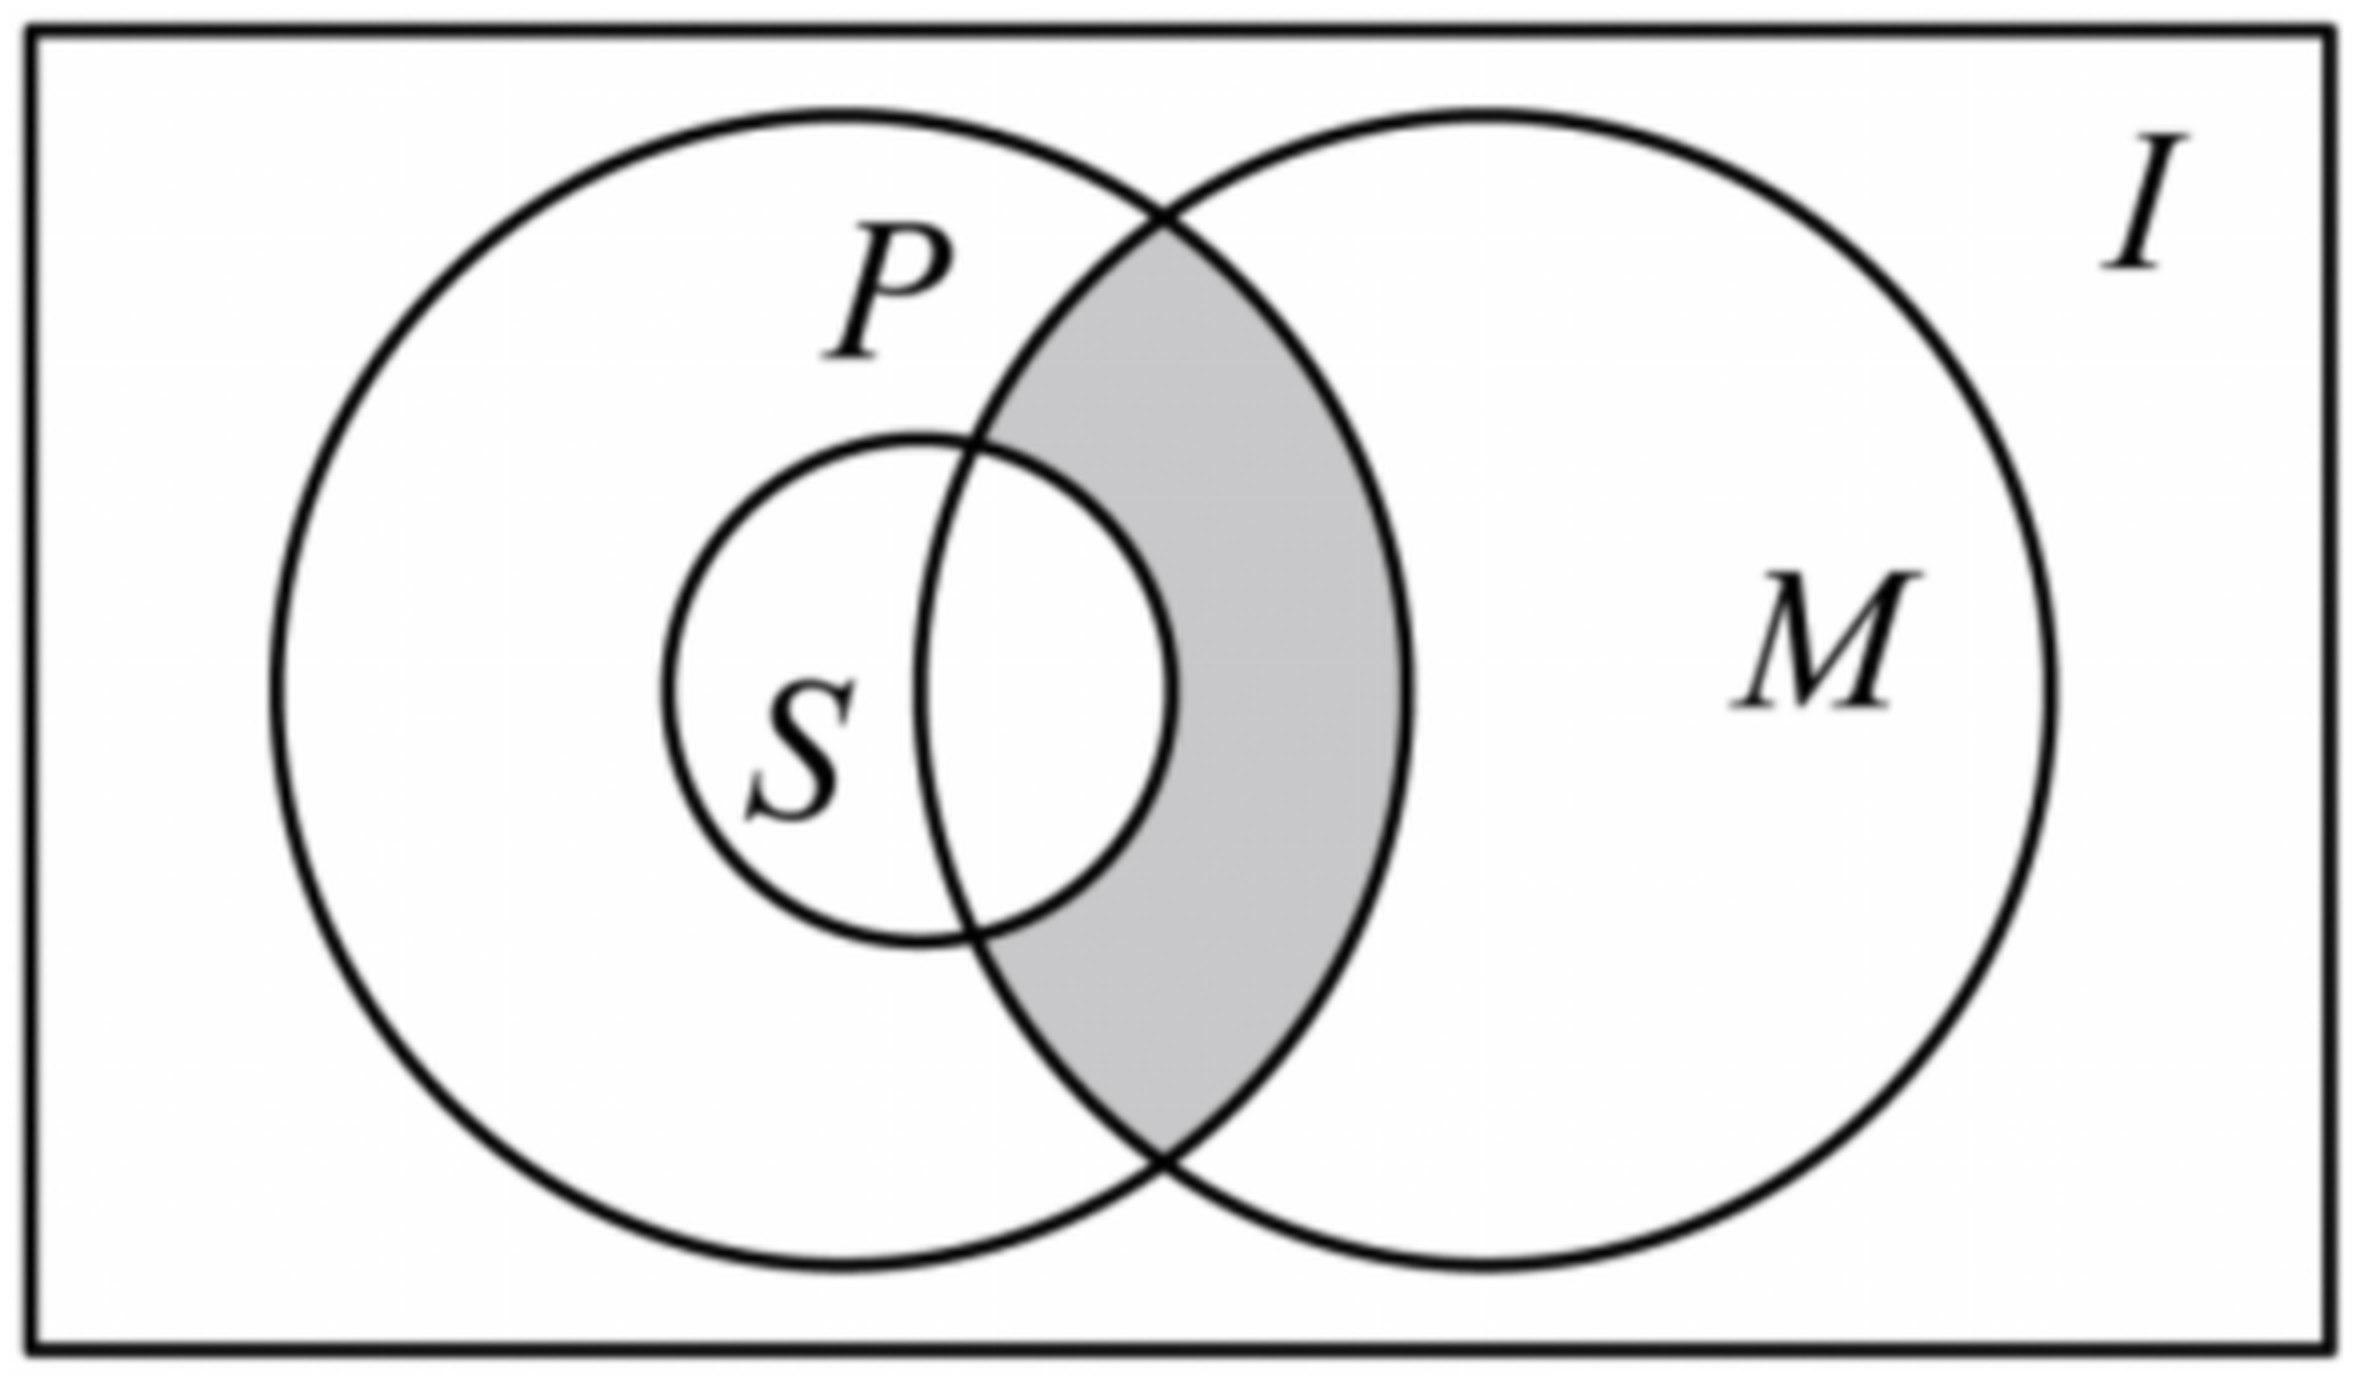
\includegraphics[width=0.46\textwidth]{figures/venn_MP_minus_S_h32.png}
\end{center}

\keepwithprev
A. $(M\cap P)\cap S$\qquad\qquad B. $(M\cap P)\cup S$

C. $(M\cap P)\cap\overline{S}$\qquad\qquad D. $(M\cap P)\cup\overline{S}$

\ans{$C$}

\ifanswer
\solbegin
\step{由 Venn 图得，集合表示 $M$、$P$ 的交集与 $S$ 的补集的交集，}
\step{即阴影部分所表示的集合是 $(M\cap P)\cap\overline{S}$. 故选 $C$.}
\solend

\fi

\item 若实数 $a$、$b$ 满足 $ab>0$，$a+2b=6$，则下列结论中错误的是\mbox{（\quad）}

\keepwithprev
A. $ab\leqslant\dfrac92$\qquad\qquad B. $a^2+4b^2\geqslant18$

C. $\dfrac1a+\dfrac2b$ 的最小值为 $\dfrac94$\qquad\qquad
D. $\dfrac{a^2}{a+1}+\dfrac{4b^2}{2b+1}$ 的最小值为 $\dfrac92$

\ans{$C$}

\ifanswer
\solbegin
\step{因为 $ab>0$，所以 $a$、$b$ 同号，又 $a+2b=6$，所以 $a$、$b$ 同正.}
\step{对于 $A$，由 $6=a+2b\geqslant2\sqrt{a\cdot2b}$ 得 $ab\leqslant\dfrac92$，故 $A$ 正确；}
\step{对于 $B$，由不等式 $\sqrt{\dfrac{m^2+n^2}2}\geqslant\dfrac{m+n}2$ 得
$\sqrt{\dfrac{a^2+(2b)^2}2}\geqslant\dfrac{a+2b}2=3$，}
\step{所以 $a^2+4b^2\geqslant18$，当且仅当 $a=2b=3$ 时取等号，故 $B$ 正确；}
\step{对于 $C$，$\dfrac1a+\dfrac2b
=\dfrac16\left(\dfrac1a+\dfrac2b\right)(a+2b)
=\dfrac16\left(5+\dfrac{2b}a+\dfrac{2a}b\right)$}
\step{$=\dfrac56+\dfrac13\left(\dfrac ba+\dfrac ab\right)
\geqslant\dfrac56+\dfrac13\times2\sqrt{\dfrac ba\cdot\dfrac ab}=\dfrac32$，}
\step{当且仅当 $\dfrac ba=\dfrac ab$，即 $a=b=2$ 时取等号，故 $C$ 错误；}
\step{对于 $D$，$\dfrac{a^2}{a+1}+\dfrac{4b^2}{2b+1}
=\dfrac{(a+1)^2-2(a+1)+1}{a+1}+\dfrac{(2b+1)^2-2(2b+1)+1}{2b+1}$}
\step{$=(a+1)-2+\dfrac1{a+1}+(2b+1)-2+\dfrac1{2b+1}
=(a+2b-2)+\dfrac1{a+1}+\dfrac1{2b+1}$}
\step{$=(6-2)+\dfrac{a+2b+2}{(a+1)(2b+1)}
=4+\dfrac8{(a+1)(2b+1)}$，}
\step{因为 $(a+1)(2b+1)\leqslant\left(\dfrac{a+1+2b+1}2\right)^2
=\left(\dfrac82\right)^2=16$，}
\step{当且仅当 $a+1=2b+1$，即 $a=2b=3$ 时取等号，}
\step{所以 $4+\dfrac8{(a+1)(2b+1)}\geqslant4+\dfrac8{16}=\dfrac92$，
故 $D$ 正确，其他几种方法同 12 题.}
\step{故选 $C$.}
\solend

\fi

% 注：本题的答案「D」原卷直接印在题干末尾的括号内，本稿按全稿惯例另提为 \ans{}。
\item 已知函数 $f(x)=x^2-2ax+a^2-1$，定义集合 $A=\{x\mid f(x)<0\}$. 若集合
$\{x\mid f(x)\in A\}=\varnothing$，则实数 $a$ 的取值范围是\mbox{（\quad）}

\keepwithprev
A. $(-3,-2)$\qquad B. $[-3,-2]$\qquad
C. $(-\infty,2)$\qquad D. $(-\infty,-2]$

\ans{$D$}

\item 非空集合 $A$ 具有如下性质：①若 $x$、$y\in A$，则 $\dfrac xy\in A$；
②若 $x$、$y\in A$，则 $x+y\in A$；

由此可知：下列判断中，错误的是\mbox{（\quad）}

\keepwithprev
A. $-1\notin A$\qquad\qquad B. $\dfrac{2025}{2026}\in A$

C. 若 $x$、$y\in A$，则 $xy\in A$\qquad\qquad
D. 若 $x$、$y\in A$，则 $x-y\in A$

\ans{$D$}

\ifanswer
\solbegin
\step{由题意得 $0\notin A$，$1\in A$，}
\step{对于 $A$，假设 $-1\in A$，则 $-1+1=0\in A$，矛盾，所以 $-1\notin A$，故 $A$ 正确；}
\step{对于 $B$，由 $1\in A$，得 $1+1=2\in A$，$2+1=3\in A$，…，$2025\in A$，$2026\in A$，}
\step{所以 $\dfrac{2025}{2026}\in A$，故 $B$ 正确；}
\step{对于 $C$，因为 $1\in A$，$x\in A$，所以 $\dfrac1x\in A$，
又因为 $y\in A$，所以 $\dfrac y{\frac1x}=xy\in A$，}
\step{故 $C$ 正确；}
\step{对于 $D$，因为 $1\in A$，$2\in A$，若 $x=1$，$y=2$，则 $x-y=-1\notin A$，故 $D$ 错误.}
\step{故选 $D$.}
\solend

\fi

\end{enumerate}

\bigsec{三、解答题}

\begin{enumerate}
\setcounter{enumi}{16}

\item 求下列关于实数 $x$ 的不等式的解集.

\begin{enumerate}[label=(\arabic*)]
\item $|2x+1|<5x-1$；
\item $\dfrac{(x-1)(x-3)(x-6)}{(x-2)(x-4)^2(x-5)}\geqslant0$.
\end{enumerate}

\ifanswer
\solbegin
\stepm{(1)}{因为不等式 $|2x+1|<5x-1$ 可化为 $-(5x-1)<2x+1<5x-1$，且 $5x-1>0$，}
\step{解得 $x>\dfrac23$，所以原不等式的解集为 $\left(\dfrac23,+\infty\right)$；}
\stepm{(2)}{不等式 $\dfrac{(x-1)(x-3)(x-6)}{(x-2)(x-4)^2(x-5)}\geqslant0$，}
\step{等价于 $(x-1)(x-3)(x-6)(x-2)(x-5)\geqslant0$，
且 $x-2\neq0$，$x-4\neq0$，$x-5\neq0$，}
\step{由“穿针引线法”，解得 $1\leqslant x<2$ 或 $3\leqslant x<4$ 或 $4<x<5$ 或 $x\geqslant6$，}
\step{所以不等式的解集为 $[1,2)\cup[3,4)\cup(4,5)\cup[6,+\infty)$.}
\solend

\fi

\ansspace[6]

\item 已知集合 $A=\left\{x\left|mx^2-mx+\dfrac{5m}2-6=0\right.\right\}\neq\varnothing$，
集合 $B=\{x\mid1<x<4$ 且 $x\in\Z\}$，$C=\{x\mid ax+3>0\}$；若 $A\cap B=A$.

\begin{enumerate}[label=(\arabic*)]
\item 求 $m$ 的取值范围.
\item 设 $m$ 的取值集合为 $D$，若 $C\cap D=\varnothing$，求 $m$ 的值及其对应 $a$ 的取值范围.
\end{enumerate}

\ans{略}

\ansspace[8]

\item 已知函数 $f(x)=x^2+(m-2)x+2m-1$.

\begin{enumerate}[label=(\arabic*)]
\item 若 $f(x)=0$ 的两根为 $x_1$、$x_2$，且 $|x_1-x_2|=2$，求实数 $m$ 的值；
\item 若函数 $y=f(x)$ 的图像在区间 $(0,1)$ 上与 $x$ 轴只有一个交点，
求实数 $m$ 的取值范围.
\end{enumerate}

\ifanswer
\solbegin
\stepm{(1)}{由题意得 $x_1+x_2=-(m-2)=2-m$，$x_1x_2=2m-1$，}
\step{由 $|x_1-x_2|=\sqrt{(x_1+x_2)^2-4x_1x_2}
=\sqrt{(2-m)^2-4(2m-1)}=2$，}
\step{化简得 $m^2-12m+4=0$，解得 $m=6\pm4\sqrt2$，故 $m=6\pm4\sqrt2$.}
\stepm{(2)}{当 $f(x)=0$ 只有一个根，且此根位于区间 $(0,1)$，}
\step{则 $\begin{cases}0<\dfrac{2-m}2<1\\[4pt]
\Delta=(m-2)^2-4(2m-1)=0\end{cases}$，
解得 $\begin{cases}0<m<2\\ m=6-2\sqrt7\text{ 或 }m=6+2\sqrt7\end{cases}$，}
\step{所以 $m=6-2\sqrt7$；}
\step{当 $f(x)=0$ 有两个根时，有一个根在区间 $(0,1)$ 内，且另一个根位于 $[0,1]$ 之外，}
\step{则 $\begin{cases}f(0)f(1)<0\\ \Delta=(m-2)^2-4(2m-1)>0\end{cases}$，
解得 $\begin{cases}\dfrac12<m<\dfrac23\\[4pt]
m<6-2\sqrt7\text{ 或 }m>6+2\sqrt7\end{cases}$，}
% 注：下一行原卷作「即 $\dfrac12<m<\dfrac32$」，按上一行方程组应为
%     $\dfrac12<m<\dfrac23$（同页最终答案也印证），照录未改，见文件头「原卷存疑」①。
\step{即 $\dfrac12<m<\dfrac32$；}
\step{当 $f(x)=0$ 有两个根位于区间 $[0,1]$ 内，且只有一个根在区间 $(0,1)$ 内，}
\step{则另一个根为 $0$ 时，得 $m=\dfrac12$，此时 $x_1+x_2=\dfrac32$，
解得另一个根 $x_2=\dfrac32>0$，故此种情况不符题意；}
\step{当 $f(x)=0$ 有两个根位于区间 $(0,1]$ 内，且只有一个根在区间 $(0,1)$ 内，}
\step{则另一个根为 $1$ 时，得 $m=\dfrac23$，此时 $x_1+x_2=\dfrac43$，
解得另一个根 $x_2=\dfrac13$，故此种情况符合题意；}
\step{综上所述，$m$ 的取值范围为
$\left(\dfrac12,\dfrac23\right]\cup\{6-2\sqrt7\}$.}
\solend

\fi

\ansspace[8]

\item 设集合 $A=\{a_1,a_2,a_3,a_4\}$，$B=\{b_1,b_2,b_3,b_4\}$，$C=\{2,3,4,6\}$，
新定义：集合 $A$ 中所有含 $k$ 个元素的子集中 $k$ 个元素之和组成的集合为“$k$ 元集和集”，
集合 $A$ 中所有含 $k$ 个元素的子集中最大元素减去剩余所有元素的和组成的集合为“$k$ 元差集”.

\begin{enumerate}[label=(\arabic*)]
\item 若 $A$ 的“$k$ 元集和集”为 $C$，求：集合 $A$.
\item 在 (1) 的条件下，若 $B$ 的“$k$ 元差集”为 $C$，求：所有满足条件的 $A\cap B$ 的真子集
个数之和.
\item 设 $b_1=a_1^2$，$b_2=a_2^2$，$b_3=a_3^2$，$b_4=a_4^2$，若 $A\cap B$ 为 $2$ 元集且
元素之和为 $10$ 且 $A$ 的“$2$ 元集和集”中最大元素不超过 $14$，求：所有满足条件的 $A$ 的
“$3$ 元差集”.
\end{enumerate}

\ifanswer
\solbegin
\stepm{(1)}{若 $A$ 的“$k$ 元集和集”为 $C$，$C=\{2,3,4,6\}$，则集合为 $\{-1,1,2,3\}$；}
\stepm{(2)}{$B$ 集合为 $\{5,3,0,-1\}$ 或 $\{9,3,1,0\}$ 或 $\{6,3,1,-1\}$，}
\step{故所有 $A\cap B$ 的真子集个数之和为 $13$；}
\stepm{(3)}{$b_1=a_1^2$，$b_2=a_2^2$，$b_3=a_3^2$，$b_4=a_4^2$，}
\step{若 $A\cap B$ 为 $2$ 元集且元素之和为 $10$，
且 $A$ 的“$2$ 元集和集”中最大元素不超过 $14$，}
% 注：下一行答案的第二个集合 $\{0,4,5,6\}$ 是 4 元集，而题问的却是「3 元差集」，
%     原卷如此，照录未改，见文件头「原卷存疑」③。
\step{则满足条件的 $A$ 的“$3$ 元差集” $\{1,3,5\}$ 或 $\{0,4,5,6\}$ 或 $\{2,4,5,8\}$.}
\solend

\fi

\ansspace[8]

\item 已知有限集 $X$、$Y$，定义集合 $X-Y=\{x\mid x\in X$ 且 $x\notin Y\}$，
$|X|$ 表示集合 $X$ 元素个数.

\begin{enumerate}[label=(\arabic*)]
\item 若 $X=\{1,2,3,4\}$，$Y=\{3,4,5\}$，写出集合 $X-Y$ 和 $Y-X$，以及
$|(X-Y)\cup(Y-X)|$ 的值；
\item 给定正整数 $n$，集合 $S=\{1,2,\cdots,n\}$，对于实数集的非空有限子集 $A$、$B$，
定义集合 $C=\{x\mid x=a+b,a\in A,b\in B\}$；

①求证：$|A-S|+|B-S|+|S-C|\geqslant1$；

②求 $|(A-S)\cup(S-A)|+|(B-S)\cup(S-B)|+|(C-S)\cup(S-C)|$ 的最小值.
\end{enumerate}

\ifanswer
\solbegin
\stepm{(1)}{由定义直接得 $X-Y=\{1,2\}$，$Y-X=\{5\}$，
$|(X-Y)\cup(Y-X)|=3$.}
% 注：下一句原卷作「显然 $|X|\geqslant0$」（按后文论证疑为 $|S|\geqslant0$），
%     照录未改，见文件头「原卷存疑」②。
\stepm{(2)}{①显然 $|X|\geqslant0$.}
\step{若 $A\cup B$ 中含有一个不在 $S$ 中的元素，则 $|A-S|+|B-S|\geqslant1$，
即 $|A-S|+|B-S|+|S-C|\geqslant1$.}
\step{若 $A\sub S$，且 $B\sub S$，则 $|A-S|=|B-S|=0$；}
\step{此时 $A$ 中最小的元素 $a\geqslant1$，$B$ 中最小的元素 $b\geqslant1$，
所以 $C$ 中最小的元素 $a+b\geqslant2$，所以 $1\notin C$.}
\step{因为 $S=\{1,2,\cdots,n\}$，所以 $|S-C|\geqslant1$，
即 $|A-S|+|B-S|+|S-C|\geqslant1$.}
\step{综上，$|A-S|+|B-S|+|S-C|\geqslant1$.}
\step{②由①得 $|A-S|+|B-S|+|S-C|\geqslant1$.}
\step{所以 $|(A-S)\cup(S-A)|+|(B-S)\cup(S-B)|+|(C-S)\cup(S-C)|$}
\step{$=|A-S|+|S-A|+|B-S|+|S-B|+|C-S|+|S-C|$}
\step{$\geqslant|S-A|+|S-B|+|C-S|+1$.}
\step{若 $A\cap S=\varnothing$，或 $B\cap S=\varnothing$，则 $|S-A|+|S-B|\geqslant n$.}
\step{若 $A\cap S\neq\varnothing$，且 $B\cap S\neq\varnothing$，
设 $A\cap S=\{a_1,a_2,\cdots,a_s\}$，$B\cap S=\{b_1,b_2,\cdots,b_t\}$，}
\step{且 $1\leqslant a_1<a_2<\cdots<a_s\leqslant n$，
$1\leqslant b_1<b_2<\cdots<b_t\leqslant n$，则 $|S-A|=n-s$，$|B-S|=n-t$.}
% 注：原卷的解析到此为止（第 10 页末），②的最小值并未给出，照录未补，
%     见文件头「原卷存疑」④。
\solend

\fi

\ansspace*[10]

\end{enumerate}

\end{document}
"
%
% 原始材料是微信公众号图文（公众号「魔都数学加油站」连载「27学年高一 32」，2026-09-25 发布，
% 原文标题「27学年高一32——2026-2027年上海市华师大二附中高一上周末作业4」），
% 正文为 10 张 PNG 页。**同一篇里各页分辨率不一致**（2560×3620 与 4762×6735 两档混排），
% 取 mmbiz.qpic.cn/<hash>/0 的原图档。原文本身就是一份**讲评版**——有的题下方印【解析】、
% 有的印【答案】，第 15 题的答案直接印在题干末尾的括号里。
% 试题文字、答案与解析均照原卷录入，未改内容。卷面的粉色斜水印属水印，未录入。
%
% ⚠ 卷首年份：本卷卷面印作「**2025-2026 年**」，与连载「27学年高一32」及公众号原文标题的
%   「2026-2027 年」**不一致**。经三人次分别把标题行裁出放大（4×—10×）独立判读，三次都读作
%   2025-2026，且校名作「华师大二附中」（无「东」字）、卷面亦无「上海市」三字。
%   按全稿「标题行照原卷」的口径，本稿照卷面排作「2025--2026 年…」——这是全稿唯一一份
%   年份不是 2026--2027 的卷子（其余 35 份均为 2026--2027）。
%
% 卷首标题：原卷印作「……年华师大二附中高一上周末作业 4」（公众号标题里的「上海市」
% 三字卷面标题行没有，本稿照卷面），年份区间按全稿惯例排 en dash，前缀照原卷保留「年」。
%
% 与原卷的排版差异（均已在 README「说明」中交代）：
%   ① 原文自**第 3 题**起（第 1、2 题未在该文中发布），故本稿题号亦自 3 起；
%   ② 原卷本就印有「一、填空题」「二、选择题」「三、解答题」三节标题，本稿照原卷分节，
%      只把标题改排成全稿统一的「大节标题」样式；
%   ③ 原卷第 6、8、9 题只印【答案】行（第 18 题的【答案】印作「略”），其余各题印【解析】，
%      第 15 题的答案直接印在题干末尾的括号内；本稿统一改为试卷版隐去、
%      答案版以 \ans{}／\ifanswer 块给出，两版彻底分离；
%   ④ 子集符号原卷两种并用：第 21(2)① 的 $A\sub S$、$B\sub S$ 带下划线，
%      第 3、10 题的 $(0,2)\subset(-\infty,3)$、$A\subset B$、$\overline{B}\subset\overline{A}$
%      作真包含，本稿分别照录为 $\sub$ 与 $\subset$；
%   ⑤ 补集符号原卷一律作上横线（$\overline{A}$、$\overline{B}$、$\overline{S}$），本稿照录；
%      空集原卷作「斜杠伸出圆外」的 $\varnothing$；
%   ⑥ 判别式记号原卷两种：第 4 题作粗体的 $\Delta$、第 11 题作细等宽的 $\triangle$，本稿照录；
%   ⑦ 数集记号原卷作斜体的 $R$、$Z$（第 4、18 题），本稿按全稿惯例统一写作 $\R$、$\Z$；
%   ⑧ 原卷填空的横线约两个字宽，本稿按全稿惯例统一排 \blankline[4.4em]；
%   ⑨ 原卷未印副标题，本稿按全稿惯例补出副标题「集合与常用逻辑用语」；
%   ⑩ 本卷只有第 13 题一图（韦恩图），原卷印在题干右侧，本稿移至题干之后；
%      图取原卷截图、4× LANCZOS 放大（figures/venn_MP_minus_S_h32.png）。
%
% 原卷存疑四处（均照抄原卷、未改，见源码中该处上方注释）：
%   ① 第 19(2)【解析】有「即 $\dfrac12<m<\dfrac32$」，按上一行的方程组应为
%      $\dfrac12<m<\dfrac23$（同页最终答案 $\left(\dfrac12,\dfrac23\right]$ 也印证）；
%   ② 第 21(2)① 首句作「显然 $|X|\geqslant0$」（按后文论证疑为 $|S|\geqslant0$）；
%   ③ 第 20(3) 的答案第二个集合 $\{0,4,5,6\}$ 是 4 元集，而题问的是「3 元差集」；
%   ④ 第 21(2)② 的解析**原卷就未写完**（第 10 页到「则 $|S-A|=n-s$，$|B-S|=n-t$」即止）。

\documentclass[a4paper,11pt]{article}
\usepackage{common}

\begin{document}

\examtitlest[3]{2025--2026 年华师大二附中高一上周末作业 4}{集合与常用逻辑用语}

\bigsec{一、填空题}

\begin{enumerate}
\setcounter{enumi}{2}

\item 设 $x$ 为实数，则“$x<3$”是“$x(x-2)<0$”的 \blankline[4.4em] 条件.

\ifanswer
\solbegin
\step{$x(x-2)<0$，解得 $0<x<2$，$(0,2)\subset(-\infty,3)$，}
\step{若 $x$ 属于“$x(x-2)<0$”，则属于“$x<3$”一定成立，即满足必要性，}
\step{若 $x$ 属于“$x<3$”，不一定满足“$x(x-2)<0$”，如 $x=-1$，即充分性不成立；}
\step{故“$x<3$”是“$x(x-2)<0$”的必要不充分条件.}
\solend

\fi

\item 若关于 $x$ 的不等式 $kx^2-kx+1>0$ 的解集为 $\R$，则实数 $k$ 的取值范围为
\blankline[4.4em].

\ifanswer
\solbegin
\step{①当 $k=0$ 时，不等式为 $1>0$ 恒成立，满足题意；}
\step{②当 $k\neq0$ 时，只要 $\begin{cases}k>0\\ \Delta=k^2-4k<0\end{cases}$，
解得 $0<k<4$；}
\step{所以不等式 $kx^2-kx+1>0$ 的解集为 $\R$，则实数 $k$ 的取值范围为 $[0,4)$.}
\solend

\fi

\item 已知 $1<a<3$，$-5<b<-2$，则 $\dfrac ab$ 的取值范围是 \blankline[4.4em].

\ifanswer
\solbegin
\step{因为 $-5<b<-2$，所以 $2<-b<5$，$\dfrac15<-\dfrac1b<\dfrac12$，又 $1<a<3$，}
\step{得 $\dfrac15<-\dfrac ab<\dfrac32$，则 $-\dfrac32<\dfrac ab<-\dfrac15$，
故 $\dfrac ab$ 的取值范围是 $\left(-\dfrac32,-\dfrac15\right)$.}
\solend

\fi

\item 关于 $x$ 的不等式 $\dfrac{ax-1}{x-a}>1$ 的解集为 $A$，且 $3\notin A$，
则实数 $a$ 的取值范围为 \blankline[4.4em].

\ans{$(-\infty,1]\cup[3,+\infty)$}

\item 若关于 $x$ 的不等式 $a\leqslant\dfrac34x^2-3x+4\leqslant b$ 的解集恰好是 $[a,b]$，
则 $b-a=$ \blankline[4.4em].

\ifanswer
\solbegin
\step{令 $f(x)=\dfrac34x^2-3x+4$，则 $f(x)$ 的对称轴为 $x=2$，}
\step{画出函数 $f(x)=\dfrac34x^2-3x+4=\dfrac34(x-2)^2+1$ 的图象，
得 $f(x)_{\min}=f(2)=1$，}
\step{由题意得 $a\leqslant1$，且 $f(a)=f(b)=b$，$a<b$，}
\step{由 $f(b)=b$ 得 $\dfrac34b^2-3b+4=b$，解得 $b=\dfrac43$（舍去）或 $b=4$，得 $b=4$，}
\step{由抛物线的对称轴为 $x=2$ 得 $a=0$，所以 $b-a=4$.}
\solend

\fi

\item 若关于 $x$ 的方程 $x^2-2kx+k+4=0$ 在 $[1,2]$ 上有解，则实数 $k$ 的取值范围为
\blankline[4.4em].

\ans{$\left[\dfrac83,5\right]$}

\item 记关于 $x$ 的方程 $x^2-2mx-2m+3=0$ 的两实根为 $x_1$、$x_2$，
则 $(x_1-2)^2+(x_2-2)^2$ 的最小值为 \blankline[4.4em].

\ans{$2$}

\item 若“$|mx^2-4x+3|\geqslant2$”的必要非充分条件是“$x\leqslant1$ 或 $x\geqslant4$”，
则实数 $m$ 的取值范围是 \blankline[4.4em].

\ifanswer
\solbegin
\step{记 $|mx^2-4x+3|\geqslant2$ 的解集为集合 $A$，
$B=\{x\mid x\leqslant1\text{ 或 }x\geqslant4\}$，}
\step{则 $\overline{A}$ 为 $|mx^2-4x+3|<2$ 的解集，$\overline{B}=\{x\mid1<x<4\}$；}
\step{因为 $B$ 是 $A$ 的必要非充分条件，所以 $A\subset B$，
得 $\overline{B}\subset\overline{A}$，}
\step{即对任意 $x\in(1,4)$，都有 $|mx^2-4x+3|<2$ 恒成立.}
\step{因为 $|mx^2-4x+3|<2$，$1<x<4$，所以 $-2<mx^2-4x+3<2$，}
\step{化简得
$-5\left(\dfrac1x\right)^2+4\left(\dfrac1x\right)
<m<-\left(\dfrac1x\right)^2+4\left(\dfrac1x\right)$；}
\step{令 $t=\dfrac1x$，$g(t)=-5t^2+4t$，$h(t)=-t^2+4t$，
且 $t\in\left(\dfrac14,1\right)$；}
\step{所以 $g(t)=-5t^2+4t=-5\left(t-\dfrac25\right)^2+\dfrac45$，
当 $t=\dfrac25$ 时，$g(t)$ 取得最大值 $\dfrac45$，}
\step{$h(t)=-t^2+4t=-(t-2)^2+4$，当 $t=\dfrac14$ 时，$h(t)$ 取得最小值，
即 $h(t)>h\left(\dfrac14\right)=\dfrac{15}{16}$；}
\step{因为对任意 $t\in\left(\dfrac14,1\right)$，$g(t)<m<h(t)$ 恒成立，
所以 $g\left(\dfrac25\right)<m\leqslant h\left(\dfrac14\right)$，}
\step{即 $\dfrac45<m\leqslant\dfrac{15}{16}$，
所以 $m$ 的取值范围是 $\left(\dfrac45,\dfrac{15}{16}\right]$.}
\solend

\fi

\item 已知关于 $x$ 的方程 $x^2+2(m-2)x+m^2-3m+3=0$ 有两个不相等的实数根 $x_1$、$x_2$，则

$\dfrac{mx_1}{x_1-1}+\dfrac{mx_2}{x_2-1}-\dfrac2{x_1+x_2-2}$ 的最大值为 \blankline[4.4em].

\ifanswer
\solbegin
\step{关于 $x$ 的方程 $x^2+2(m-2)x+m^2-3m+3=0$ 有两个不相等的实数根 $x_1$、$x_2$，}
\step{则 $\triangle=4(m-2)^2-4(m^2-3m+3)=-4m+4>0$，得 $m<1$，}
\step{且 $x_1+x_2=-2(m-2)$，$x_1x_2=m^2-3m+3$，}
\step{$\dfrac{mx_1}{x_1-1}+\dfrac{mx_2}{x_2-1}-\dfrac2{x_1+x_2-2}
=\dfrac{m[2x_1x_2-(x_1+x_2)]}{x_1x_2-(x_1+x_2)+1}+\dfrac1{m-1}$}
\step{$=\dfrac{2m(m-1)^2}{m^2-m}+\dfrac1{m-1}=2(m-1)+\dfrac1{m-1}$，}
\step{又因为 $m<1$，所以 $m-1<0$，则 $1-m>0$，}
\step{所以 $2(1-m)+\dfrac1{1-m}\geqslant2\sqrt{2(1-m)\cdot\dfrac1{1-m}}=2\sqrt2$，}
\step{当且仅当 $2(1-m)=\dfrac1{1-m}$ 时，即 $m=1-\dfrac{\sqrt2}2$ 时取等号，}
\step{所以 $2(m-1)+\dfrac1{m-1}\leqslant-2\sqrt2$，
即 $\dfrac{mx_1}{x_1-1}+\dfrac{mx_2}{x_2-1}-\dfrac2{x_1+x_2-2}$ 的最大值为 $-2\sqrt2$.}
\solend

\fi

\item 若正实数 $a$、$b$ 满足 $a+2b=ab$，则 $\dfrac4{a^2+2a}+\dfrac1{2b^2+b}$ 的最小值是
\blankline[4.4em].

\ifanswer
\solbegin
\stepm{法一}{由 $a+2b=ab$，得 $\dfrac2a+\dfrac1b=1$，}
\step{令 $x=\dfrac1a$，$y=\dfrac1b$，则 $x$、$y>0$，$2x+y=1$，$2x+1+y+2=4$，}
\step{所以 $\dfrac4{a^2+2a}+\dfrac1{2b^2+b}
=\dfrac4{\frac1{x^2}+\frac2x}+\dfrac1{\frac2{y^2}+\frac1y}
=\dfrac{4x^2}{2x+1}+\dfrac{y^2}{y+2}$（*）}
\step{$=\dfrac{(2x+1)^2-2(2x+1)+1}{2x+1}+\dfrac{(y+2)^2-4(y+2)+4}{y+2}$}
\step{$=2x-1+\dfrac1{2x+1}+y-2+\dfrac4{y+2}=\dfrac1{2x+1}+\dfrac4{y+2}-2$}
\step{$=\dfrac14\left(\dfrac1{2x+1}+\dfrac4{y+2}\right)(2x+1+y+2)-2$}
\step{$=\dfrac14\left[5+\dfrac{y+2}{2x+1}+\dfrac{4(2x+1)}{y+2}\right]-2
\geqslant\dfrac14(5+2\sqrt4)-2=\dfrac14$，}
\step{当且仅当 $\dfrac{y+2}{2x+1}=\dfrac{4(2x+1)}{y+2}$，
即 $x=\dfrac16$，$y=\dfrac23$ 时取等号，}
\step{故 $\dfrac4{a^2+2a}+\dfrac1{2b^2+b}$ 的最小值是 $\dfrac14$.}
\stepm{法二}{在法一（*）后，由权方和不等式，得
$\dfrac4{a^2+2a}+\dfrac1{2b^2+b}
=\dfrac{4x^2}{2x+1}+\dfrac{y^2}{y+2}
\geqslant\dfrac{(2x+y)^2}{2x+1+y+2}=\dfrac14$，}
\step{当且仅当……，故 $\dfrac4{a^2+2a}+\dfrac1{2b^2+b}$ 的最小值是 $\dfrac14$.}
\stepm{法三}{注意到
$\left(\dfrac{a+2}a+\dfrac{2b+1}b\right)\left(\dfrac4{a^2+2a}+\dfrac1{2b^2+b}\right)$}
\step{$\geqslant
\left(\sqrt{\dfrac{a+2}a\cdot\dfrac4{a^2+2a}}
+\sqrt{\dfrac{2b+1}b\cdot\dfrac1{2b^2+b}}\right)^2
=\left(\dfrac2a+\dfrac1b\right)^2$，}
\step{其中 $\dfrac{a+2}a+\dfrac{2b+1}b=3+\dfrac{a+2b}{ab}=4$，
$\dfrac2a+\dfrac1b=\dfrac{a+2b}{ab}=1$，}
\step{所以 $\dfrac4{a^2+2a}+\dfrac1{2b^2+b}\geqslant\dfrac14$，
当且仅当……，故 $\dfrac4{a^2+2a}+\dfrac1{2b^2+b}$ 的最小值是 $\dfrac14$.}
\solend

\fi

\end{enumerate}

\bigsec{二、选择题}

\begin{enumerate}
\setcounter{enumi}{12}

\item 如图，$I$ 为全集，$M$、$P$、$S$ 是 $I$ 的三个子集，则阴影部分所表示的集合是
\mbox{（\quad）}

\begin{center}
% 图取原卷截图、4× LANCZOS 放大（原卷把图印在题干右侧，本稿移至此处，见文件头⑩）。
% 矩形为全集 $I$，左大圆 $P$（内下方含小圆 $S$，其右侧伸入 $P$ 与 $M$ 的重叠区）、
% 右大圆 $M$；阴影是 $P$、$M$ 重叠的透镜形区域挖掉 $S$ 后剩下的部分（左缘呈弯月形）。
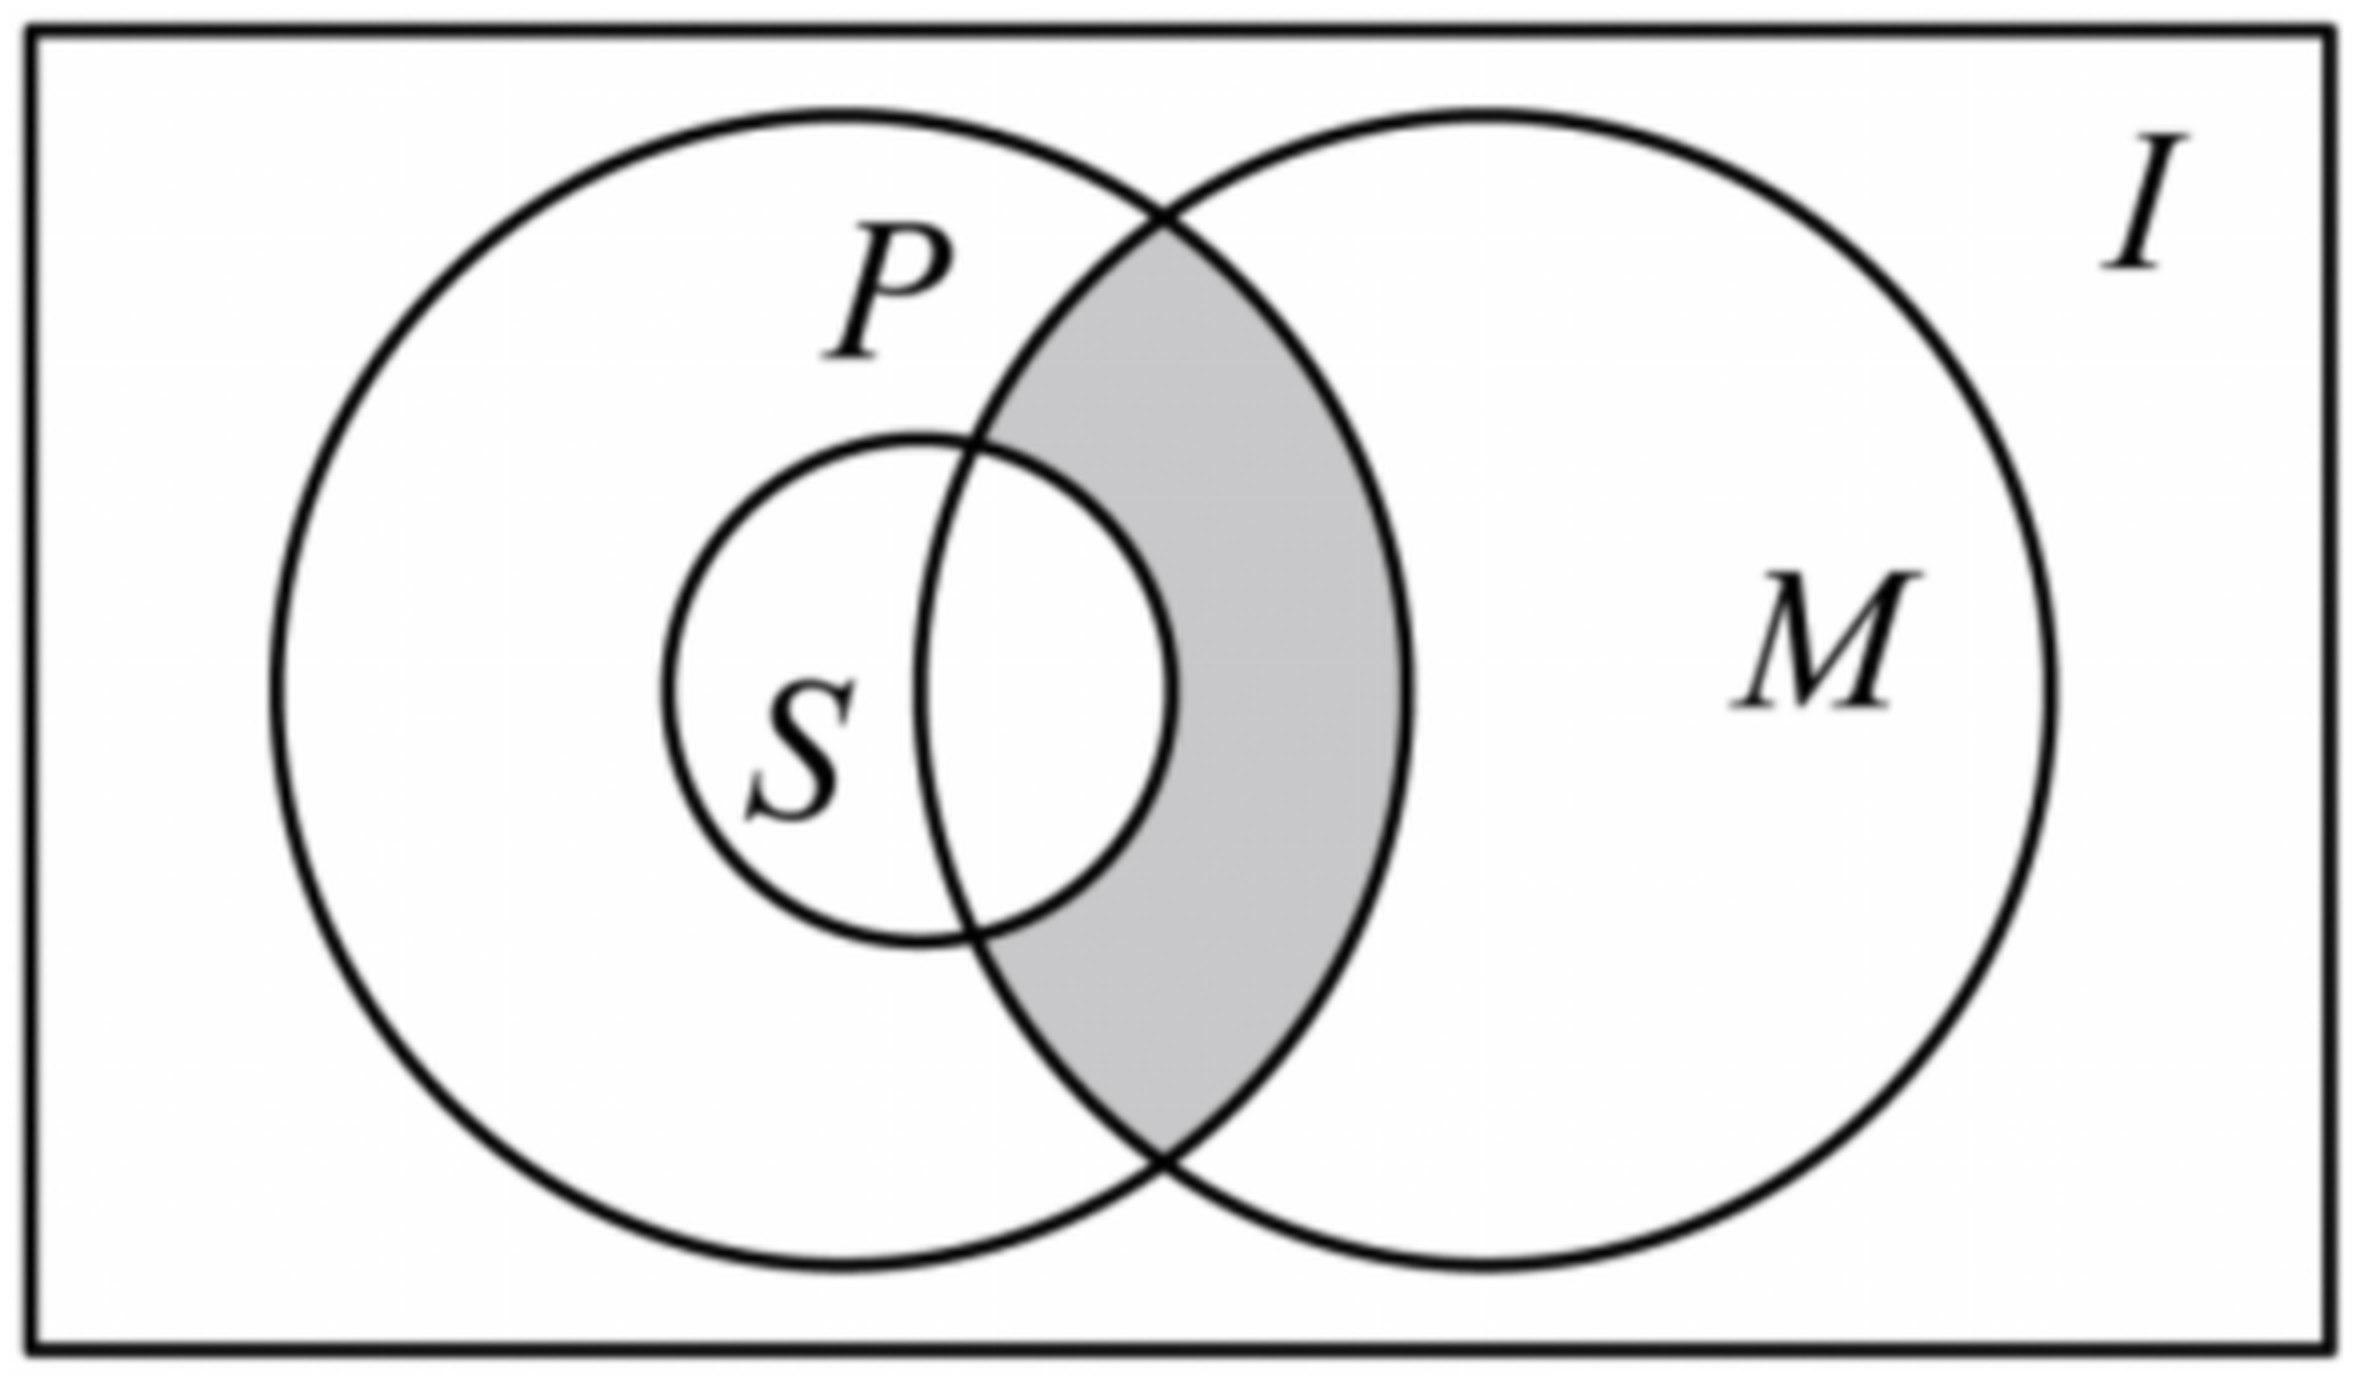
\includegraphics[width=0.46\textwidth]{figures/venn_MP_minus_S_h32.png}
\end{center}

\keepwithprev
A. $(M\cap P)\cap S$\qquad\qquad B. $(M\cap P)\cup S$

C. $(M\cap P)\cap\overline{S}$\qquad\qquad D. $(M\cap P)\cup\overline{S}$

\ans{$C$}

\ifanswer
\solbegin
\step{由 Venn 图得，集合表示 $M$、$P$ 的交集与 $S$ 的补集的交集，}
\step{即阴影部分所表示的集合是 $(M\cap P)\cap\overline{S}$. 故选 $C$.}
\solend

\fi

\item 若实数 $a$、$b$ 满足 $ab>0$，$a+2b=6$，则下列结论中错误的是\mbox{（\quad）}

\keepwithprev
A. $ab\leqslant\dfrac92$\qquad\qquad B. $a^2+4b^2\geqslant18$

C. $\dfrac1a+\dfrac2b$ 的最小值为 $\dfrac94$\qquad\qquad
D. $\dfrac{a^2}{a+1}+\dfrac{4b^2}{2b+1}$ 的最小值为 $\dfrac92$

\ans{$C$}

\ifanswer
\solbegin
\step{因为 $ab>0$，所以 $a$、$b$ 同号，又 $a+2b=6$，所以 $a$、$b$ 同正.}
\step{对于 $A$，由 $6=a+2b\geqslant2\sqrt{a\cdot2b}$ 得 $ab\leqslant\dfrac92$，故 $A$ 正确；}
\step{对于 $B$，由不等式 $\sqrt{\dfrac{m^2+n^2}2}\geqslant\dfrac{m+n}2$ 得
$\sqrt{\dfrac{a^2+(2b)^2}2}\geqslant\dfrac{a+2b}2=3$，}
\step{所以 $a^2+4b^2\geqslant18$，当且仅当 $a=2b=3$ 时取等号，故 $B$ 正确；}
\step{对于 $C$，$\dfrac1a+\dfrac2b
=\dfrac16\left(\dfrac1a+\dfrac2b\right)(a+2b)
=\dfrac16\left(5+\dfrac{2b}a+\dfrac{2a}b\right)$}
\step{$=\dfrac56+\dfrac13\left(\dfrac ba+\dfrac ab\right)
\geqslant\dfrac56+\dfrac13\times2\sqrt{\dfrac ba\cdot\dfrac ab}=\dfrac32$，}
\step{当且仅当 $\dfrac ba=\dfrac ab$，即 $a=b=2$ 时取等号，故 $C$ 错误；}
\step{对于 $D$，$\dfrac{a^2}{a+1}+\dfrac{4b^2}{2b+1}
=\dfrac{(a+1)^2-2(a+1)+1}{a+1}+\dfrac{(2b+1)^2-2(2b+1)+1}{2b+1}$}
\step{$=(a+1)-2+\dfrac1{a+1}+(2b+1)-2+\dfrac1{2b+1}
=(a+2b-2)+\dfrac1{a+1}+\dfrac1{2b+1}$}
\step{$=(6-2)+\dfrac{a+2b+2}{(a+1)(2b+1)}
=4+\dfrac8{(a+1)(2b+1)}$，}
\step{因为 $(a+1)(2b+1)\leqslant\left(\dfrac{a+1+2b+1}2\right)^2
=\left(\dfrac82\right)^2=16$，}
\step{当且仅当 $a+1=2b+1$，即 $a=2b=3$ 时取等号，}
\step{所以 $4+\dfrac8{(a+1)(2b+1)}\geqslant4+\dfrac8{16}=\dfrac92$，
故 $D$ 正确，其他几种方法同 12 题.}
\step{故选 $C$.}
\solend

\fi

% 注：本题的答案「D」原卷直接印在题干末尾的括号内，本稿按全稿惯例另提为 \ans{}。
\item 已知函数 $f(x)=x^2-2ax+a^2-1$，定义集合 $A=\{x\mid f(x)<0\}$. 若集合
$\{x\mid f(x)\in A\}=\varnothing$，则实数 $a$ 的取值范围是\mbox{（\quad）}

\keepwithprev
A. $(-3,-2)$\qquad B. $[-3,-2]$\qquad
C. $(-\infty,2)$\qquad D. $(-\infty,-2]$

\ans{$D$}

\item 非空集合 $A$ 具有如下性质：①若 $x$、$y\in A$，则 $\dfrac xy\in A$；
②若 $x$、$y\in A$，则 $x+y\in A$；

由此可知：下列判断中，错误的是\mbox{（\quad）}

\keepwithprev
A. $-1\notin A$\qquad\qquad B. $\dfrac{2025}{2026}\in A$

C. 若 $x$、$y\in A$，则 $xy\in A$\qquad\qquad
D. 若 $x$、$y\in A$，则 $x-y\in A$

\ans{$D$}

\ifanswer
\solbegin
\step{由题意得 $0\notin A$，$1\in A$，}
\step{对于 $A$，假设 $-1\in A$，则 $-1+1=0\in A$，矛盾，所以 $-1\notin A$，故 $A$ 正确；}
\step{对于 $B$，由 $1\in A$，得 $1+1=2\in A$，$2+1=3\in A$，…，$2025\in A$，$2026\in A$，}
\step{所以 $\dfrac{2025}{2026}\in A$，故 $B$ 正确；}
\step{对于 $C$，因为 $1\in A$，$x\in A$，所以 $\dfrac1x\in A$，
又因为 $y\in A$，所以 $\dfrac y{\frac1x}=xy\in A$，}
\step{故 $C$ 正确；}
\step{对于 $D$，因为 $1\in A$，$2\in A$，若 $x=1$，$y=2$，则 $x-y=-1\notin A$，故 $D$ 错误.}
\step{故选 $D$.}
\solend

\fi

\end{enumerate}

\bigsec{三、解答题}

\begin{enumerate}
\setcounter{enumi}{16}

\item 求下列关于实数 $x$ 的不等式的解集.

\begin{enumerate}[label=(\arabic*)]
\item $|2x+1|<5x-1$；
\item $\dfrac{(x-1)(x-3)(x-6)}{(x-2)(x-4)^2(x-5)}\geqslant0$.
\end{enumerate}

\ifanswer
\solbegin
\stepm{(1)}{因为不等式 $|2x+1|<5x-1$ 可化为 $-(5x-1)<2x+1<5x-1$，且 $5x-1>0$，}
\step{解得 $x>\dfrac23$，所以原不等式的解集为 $\left(\dfrac23,+\infty\right)$；}
\stepm{(2)}{不等式 $\dfrac{(x-1)(x-3)(x-6)}{(x-2)(x-4)^2(x-5)}\geqslant0$，}
\step{等价于 $(x-1)(x-3)(x-6)(x-2)(x-5)\geqslant0$，
且 $x-2\neq0$，$x-4\neq0$，$x-5\neq0$，}
\step{由“穿针引线法”，解得 $1\leqslant x<2$ 或 $3\leqslant x<4$ 或 $4<x<5$ 或 $x\geqslant6$，}
\step{所以不等式的解集为 $[1,2)\cup[3,4)\cup(4,5)\cup[6,+\infty)$.}
\solend

\fi

\ansspace[6]

\item 已知集合 $A=\left\{x\left|mx^2-mx+\dfrac{5m}2-6=0\right.\right\}\neq\varnothing$，
集合 $B=\{x\mid1<x<4$ 且 $x\in\Z\}$，$C=\{x\mid ax+3>0\}$；若 $A\cap B=A$.

\begin{enumerate}[label=(\arabic*)]
\item 求 $m$ 的取值范围.
\item 设 $m$ 的取值集合为 $D$，若 $C\cap D=\varnothing$，求 $m$ 的值及其对应 $a$ 的取值范围.
\end{enumerate}

\ans{略}

\ansspace[8]

\item 已知函数 $f(x)=x^2+(m-2)x+2m-1$.

\begin{enumerate}[label=(\arabic*)]
\item 若 $f(x)=0$ 的两根为 $x_1$、$x_2$，且 $|x_1-x_2|=2$，求实数 $m$ 的值；
\item 若函数 $y=f(x)$ 的图像在区间 $(0,1)$ 上与 $x$ 轴只有一个交点，
求实数 $m$ 的取值范围.
\end{enumerate}

\ifanswer
\solbegin
\stepm{(1)}{由题意得 $x_1+x_2=-(m-2)=2-m$，$x_1x_2=2m-1$，}
\step{由 $|x_1-x_2|=\sqrt{(x_1+x_2)^2-4x_1x_2}
=\sqrt{(2-m)^2-4(2m-1)}=2$，}
\step{化简得 $m^2-12m+4=0$，解得 $m=6\pm4\sqrt2$，故 $m=6\pm4\sqrt2$.}
\stepm{(2)}{当 $f(x)=0$ 只有一个根，且此根位于区间 $(0,1)$，}
\step{则 $\begin{cases}0<\dfrac{2-m}2<1\\[4pt]
\Delta=(m-2)^2-4(2m-1)=0\end{cases}$，
解得 $\begin{cases}0<m<2\\ m=6-2\sqrt7\text{ 或 }m=6+2\sqrt7\end{cases}$，}
\step{所以 $m=6-2\sqrt7$；}
\step{当 $f(x)=0$ 有两个根时，有一个根在区间 $(0,1)$ 内，且另一个根位于 $[0,1]$ 之外，}
\step{则 $\begin{cases}f(0)f(1)<0\\ \Delta=(m-2)^2-4(2m-1)>0\end{cases}$，
解得 $\begin{cases}\dfrac12<m<\dfrac23\\[4pt]
m<6-2\sqrt7\text{ 或 }m>6+2\sqrt7\end{cases}$，}
% 注：下一行原卷作「即 $\dfrac12<m<\dfrac32$」，按上一行方程组应为
%     $\dfrac12<m<\dfrac23$（同页最终答案也印证），照录未改，见文件头「原卷存疑」①。
\step{即 $\dfrac12<m<\dfrac32$；}
\step{当 $f(x)=0$ 有两个根位于区间 $[0,1]$ 内，且只有一个根在区间 $(0,1)$ 内，}
\step{则另一个根为 $0$ 时，得 $m=\dfrac12$，此时 $x_1+x_2=\dfrac32$，
解得另一个根 $x_2=\dfrac32>0$，故此种情况不符题意；}
\step{当 $f(x)=0$ 有两个根位于区间 $(0,1]$ 内，且只有一个根在区间 $(0,1)$ 内，}
\step{则另一个根为 $1$ 时，得 $m=\dfrac23$，此时 $x_1+x_2=\dfrac43$，
解得另一个根 $x_2=\dfrac13$，故此种情况符合题意；}
\step{综上所述，$m$ 的取值范围为
$\left(\dfrac12,\dfrac23\right]\cup\{6-2\sqrt7\}$.}
\solend

\fi

\ansspace[8]

\item 设集合 $A=\{a_1,a_2,a_3,a_4\}$，$B=\{b_1,b_2,b_3,b_4\}$，$C=\{2,3,4,6\}$，
新定义：集合 $A$ 中所有含 $k$ 个元素的子集中 $k$ 个元素之和组成的集合为“$k$ 元集和集”，
集合 $A$ 中所有含 $k$ 个元素的子集中最大元素减去剩余所有元素的和组成的集合为“$k$ 元差集”.

\begin{enumerate}[label=(\arabic*)]
\item 若 $A$ 的“$k$ 元集和集”为 $C$，求：集合 $A$.
\item 在 (1) 的条件下，若 $B$ 的“$k$ 元差集”为 $C$，求：所有满足条件的 $A\cap B$ 的真子集
个数之和.
\item 设 $b_1=a_1^2$，$b_2=a_2^2$，$b_3=a_3^2$，$b_4=a_4^2$，若 $A\cap B$ 为 $2$ 元集且
元素之和为 $10$ 且 $A$ 的“$2$ 元集和集”中最大元素不超过 $14$，求：所有满足条件的 $A$ 的
“$3$ 元差集”.
\end{enumerate}

\ifanswer
\solbegin
\stepm{(1)}{若 $A$ 的“$k$ 元集和集”为 $C$，$C=\{2,3,4,6\}$，则集合为 $\{-1,1,2,3\}$；}
\stepm{(2)}{$B$ 集合为 $\{5,3,0,-1\}$ 或 $\{9,3,1,0\}$ 或 $\{6,3,1,-1\}$，}
\step{故所有 $A\cap B$ 的真子集个数之和为 $13$；}
\stepm{(3)}{$b_1=a_1^2$，$b_2=a_2^2$，$b_3=a_3^2$，$b_4=a_4^2$，}
\step{若 $A\cap B$ 为 $2$ 元集且元素之和为 $10$，
且 $A$ 的“$2$ 元集和集”中最大元素不超过 $14$，}
% 注：下一行答案的第二个集合 $\{0,4,5,6\}$ 是 4 元集，而题问的却是「3 元差集」，
%     原卷如此，照录未改，见文件头「原卷存疑」③。
\step{则满足条件的 $A$ 的“$3$ 元差集” $\{1,3,5\}$ 或 $\{0,4,5,6\}$ 或 $\{2,4,5,8\}$.}
\solend

\fi

\ansspace[8]

\item 已知有限集 $X$、$Y$，定义集合 $X-Y=\{x\mid x\in X$ 且 $x\notin Y\}$，
$|X|$ 表示集合 $X$ 元素个数.

\begin{enumerate}[label=(\arabic*)]
\item 若 $X=\{1,2,3,4\}$，$Y=\{3,4,5\}$，写出集合 $X-Y$ 和 $Y-X$，以及
$|(X-Y)\cup(Y-X)|$ 的值；
\item 给定正整数 $n$，集合 $S=\{1,2,\cdots,n\}$，对于实数集的非空有限子集 $A$、$B$，
定义集合 $C=\{x\mid x=a+b,a\in A,b\in B\}$；

①求证：$|A-S|+|B-S|+|S-C|\geqslant1$；

②求 $|(A-S)\cup(S-A)|+|(B-S)\cup(S-B)|+|(C-S)\cup(S-C)|$ 的最小值.
\end{enumerate}

\ifanswer
\solbegin
\stepm{(1)}{由定义直接得 $X-Y=\{1,2\}$，$Y-X=\{5\}$，
$|(X-Y)\cup(Y-X)|=3$.}
% 注：下一句原卷作「显然 $|X|\geqslant0$」（按后文论证疑为 $|S|\geqslant0$），
%     照录未改，见文件头「原卷存疑」②。
\stepm{(2)}{①显然 $|X|\geqslant0$.}
\step{若 $A\cup B$ 中含有一个不在 $S$ 中的元素，则 $|A-S|+|B-S|\geqslant1$，
即 $|A-S|+|B-S|+|S-C|\geqslant1$.}
\step{若 $A\sub S$，且 $B\sub S$，则 $|A-S|=|B-S|=0$；}
\step{此时 $A$ 中最小的元素 $a\geqslant1$，$B$ 中最小的元素 $b\geqslant1$，
所以 $C$ 中最小的元素 $a+b\geqslant2$，所以 $1\notin C$.}
\step{因为 $S=\{1,2,\cdots,n\}$，所以 $|S-C|\geqslant1$，
即 $|A-S|+|B-S|+|S-C|\geqslant1$.}
\step{综上，$|A-S|+|B-S|+|S-C|\geqslant1$.}
\step{②由①得 $|A-S|+|B-S|+|S-C|\geqslant1$.}
\step{所以 $|(A-S)\cup(S-A)|+|(B-S)\cup(S-B)|+|(C-S)\cup(S-C)|$}
\step{$=|A-S|+|S-A|+|B-S|+|S-B|+|C-S|+|S-C|$}
\step{$\geqslant|S-A|+|S-B|+|C-S|+1$.}
\step{若 $A\cap S=\varnothing$，或 $B\cap S=\varnothing$，则 $|S-A|+|S-B|\geqslant n$.}
\step{若 $A\cap S\neq\varnothing$，且 $B\cap S\neq\varnothing$，
设 $A\cap S=\{a_1,a_2,\cdots,a_s\}$，$B\cap S=\{b_1,b_2,\cdots,b_t\}$，}
\step{且 $1\leqslant a_1<a_2<\cdots<a_s\leqslant n$，
$1\leqslant b_1<b_2<\cdots<b_t\leqslant n$，则 $|S-A|=n-s$，$|B-S|=n-t$.}
% 注：原卷的解析到此为止（第 10 页末），②的最小值并未给出，照录未补，
%     见文件头「原卷存疑」④。
\solend

\fi

\ansspace*[10]

\end{enumerate}

\end{document}
"
%
% 原始材料是微信公众号图文（公众号「魔都数学加油站」连载「27学年高一 32」，2026-09-25 发布，
% 原文标题「27学年高一32——2026-2027年上海市华师大二附中高一上周末作业4」），
% 正文为 10 张 PNG 页。**同一篇里各页分辨率不一致**（2560×3620 与 4762×6735 两档混排），
% 取 mmbiz.qpic.cn/<hash>/0 的原图档。原文本身就是一份**讲评版**——有的题下方印【解析】、
% 有的印【答案】，第 15 题的答案直接印在题干末尾的括号里。
% 试题文字、答案与解析均照原卷录入，未改内容。卷面的粉色斜水印属水印，未录入。
%
% ⚠ 卷首年份：本卷卷面印作「**2025-2026 年**」，与连载「27学年高一32」及公众号原文标题的
%   「2026-2027 年」**不一致**。经三人次分别把标题行裁出放大（4×—10×）独立判读，三次都读作
%   2025-2026，且校名作「华师大二附中」（无「东」字）、卷面亦无「上海市」三字。
%   按全稿「标题行照原卷」的口径，本稿照卷面排作「2025--2026 年…」——这是全稿唯一一份
%   年份不是 2026--2027 的卷子（其余 35 份均为 2026--2027）。
%
% 卷首标题：原卷印作「……年华师大二附中高一上周末作业 4」（公众号标题里的「上海市」
% 三字卷面标题行没有，本稿照卷面），年份区间按全稿惯例排 en dash，前缀照原卷保留「年」。
%
% 与原卷的排版差异（均已在 README「说明」中交代）：
%   ① 原文自**第 3 题**起（第 1、2 题未在该文中发布），故本稿题号亦自 3 起；
%   ② 原卷本就印有「一、填空题」「二、选择题」「三、解答题」三节标题，本稿照原卷分节，
%      只把标题改排成全稿统一的「大节标题」样式；
%   ③ 原卷第 6、8、9 题只印【答案】行（第 18 题的【答案】印作「略”），其余各题印【解析】，
%      第 15 题的答案直接印在题干末尾的括号内；本稿统一改为试卷版隐去、
%      答案版以 \ans{}／\ifanswer 块给出，两版彻底分离；
%   ④ 子集符号原卷两种并用：第 21(2)① 的 $A\sub S$、$B\sub S$ 带下划线，
%      第 3、10 题的 $(0,2)\subset(-\infty,3)$、$A\subset B$、$\overline{B}\subset\overline{A}$
%      作真包含，本稿分别照录为 $\sub$ 与 $\subset$；
%   ⑤ 补集符号原卷一律作上横线（$\overline{A}$、$\overline{B}$、$\overline{S}$），本稿照录；
%      空集原卷作「斜杠伸出圆外」的 $\varnothing$；
%   ⑥ 判别式记号原卷两种：第 4 题作粗体的 $\Delta$、第 11 题作细等宽的 $\triangle$，本稿照录；
%   ⑦ 数集记号原卷作斜体的 $R$、$Z$（第 4、18 题），本稿按全稿惯例统一写作 $\R$、$\Z$；
%   ⑧ 原卷填空的横线约两个字宽，本稿按全稿惯例统一排 \blankline[4.4em]；
%   ⑨ 原卷未印副标题，本稿按全稿惯例补出副标题「集合与常用逻辑用语」；
%   ⑩ 本卷只有第 13 题一图（韦恩图），原卷印在题干右侧，本稿移至题干之后；
%      图取原卷截图、4× LANCZOS 放大（figures/venn_MP_minus_S_h32.png）。
%
% 原卷存疑四处（均照抄原卷、未改，见源码中该处上方注释）：
%   ① 第 19(2)【解析】有「即 $\dfrac12<m<\dfrac32$」，按上一行的方程组应为
%      $\dfrac12<m<\dfrac23$（同页最终答案 $\left(\dfrac12,\dfrac23\right]$ 也印证）；
%   ② 第 21(2)① 首句作「显然 $|X|\geqslant0$」（按后文论证疑为 $|S|\geqslant0$）；
%   ③ 第 20(3) 的答案第二个集合 $\{0,4,5,6\}$ 是 4 元集，而题问的是「3 元差集」；
%   ④ 第 21(2)② 的解析**原卷就未写完**（第 10 页到「则 $|S-A|=n-s$，$|B-S|=n-t$」即止）。

\documentclass[a4paper,11pt]{article}
\usepackage{common}

\begin{document}

\examtitlest[3]{2025--2026 年华师大二附中高一上周末作业 4}{集合与常用逻辑用语}

\bigsec{一、填空题}

\begin{enumerate}
\setcounter{enumi}{2}

\item 设 $x$ 为实数，则“$x<3$”是“$x(x-2)<0$”的 \blankline[4.4em] 条件.

\ifanswer
\solbegin
\step{$x(x-2)<0$，解得 $0<x<2$，$(0,2)\subset(-\infty,3)$，}
\step{若 $x$ 属于“$x(x-2)<0$”，则属于“$x<3$”一定成立，即满足必要性，}
\step{若 $x$ 属于“$x<3$”，不一定满足“$x(x-2)<0$”，如 $x=-1$，即充分性不成立；}
\step{故“$x<3$”是“$x(x-2)<0$”的必要不充分条件.}
\solend

\fi

\item 若关于 $x$ 的不等式 $kx^2-kx+1>0$ 的解集为 $\R$，则实数 $k$ 的取值范围为
\blankline[4.4em].

\ifanswer
\solbegin
\step{①当 $k=0$ 时，不等式为 $1>0$ 恒成立，满足题意；}
\step{②当 $k\neq0$ 时，只要 $\begin{cases}k>0\\ \Delta=k^2-4k<0\end{cases}$，
解得 $0<k<4$；}
\step{所以不等式 $kx^2-kx+1>0$ 的解集为 $\R$，则实数 $k$ 的取值范围为 $[0,4)$.}
\solend

\fi

\item 已知 $1<a<3$，$-5<b<-2$，则 $\dfrac ab$ 的取值范围是 \blankline[4.4em].

\ifanswer
\solbegin
\step{因为 $-5<b<-2$，所以 $2<-b<5$，$\dfrac15<-\dfrac1b<\dfrac12$，又 $1<a<3$，}
\step{得 $\dfrac15<-\dfrac ab<\dfrac32$，则 $-\dfrac32<\dfrac ab<-\dfrac15$，
故 $\dfrac ab$ 的取值范围是 $\left(-\dfrac32,-\dfrac15\right)$.}
\solend

\fi

\item 关于 $x$ 的不等式 $\dfrac{ax-1}{x-a}>1$ 的解集为 $A$，且 $3\notin A$，
则实数 $a$ 的取值范围为 \blankline[4.4em].

\ans{$(-\infty,1]\cup[3,+\infty)$}

\item 若关于 $x$ 的不等式 $a\leqslant\dfrac34x^2-3x+4\leqslant b$ 的解集恰好是 $[a,b]$，
则 $b-a=$ \blankline[4.4em].

\ifanswer
\solbegin
\step{令 $f(x)=\dfrac34x^2-3x+4$，则 $f(x)$ 的对称轴为 $x=2$，}
\step{画出函数 $f(x)=\dfrac34x^2-3x+4=\dfrac34(x-2)^2+1$ 的图象，
得 $f(x)_{\min}=f(2)=1$，}
\step{由题意得 $a\leqslant1$，且 $f(a)=f(b)=b$，$a<b$，}
\step{由 $f(b)=b$ 得 $\dfrac34b^2-3b+4=b$，解得 $b=\dfrac43$（舍去）或 $b=4$，得 $b=4$，}
\step{由抛物线的对称轴为 $x=2$ 得 $a=0$，所以 $b-a=4$.}
\solend

\fi

\item 若关于 $x$ 的方程 $x^2-2kx+k+4=0$ 在 $[1,2]$ 上有解，则实数 $k$ 的取值范围为
\blankline[4.4em].

\ans{$\left[\dfrac83,5\right]$}

\item 记关于 $x$ 的方程 $x^2-2mx-2m+3=0$ 的两实根为 $x_1$、$x_2$，
则 $(x_1-2)^2+(x_2-2)^2$ 的最小值为 \blankline[4.4em].

\ans{$2$}

\item 若“$|mx^2-4x+3|\geqslant2$”的必要非充分条件是“$x\leqslant1$ 或 $x\geqslant4$”，
则实数 $m$ 的取值范围是 \blankline[4.4em].

\ifanswer
\solbegin
\step{记 $|mx^2-4x+3|\geqslant2$ 的解集为集合 $A$，
$B=\{x\mid x\leqslant1\text{ 或 }x\geqslant4\}$，}
\step{则 $\overline{A}$ 为 $|mx^2-4x+3|<2$ 的解集，$\overline{B}=\{x\mid1<x<4\}$；}
\step{因为 $B$ 是 $A$ 的必要非充分条件，所以 $A\subset B$，
得 $\overline{B}\subset\overline{A}$，}
\step{即对任意 $x\in(1,4)$，都有 $|mx^2-4x+3|<2$ 恒成立.}
\step{因为 $|mx^2-4x+3|<2$，$1<x<4$，所以 $-2<mx^2-4x+3<2$，}
\step{化简得
$-5\left(\dfrac1x\right)^2+4\left(\dfrac1x\right)
<m<-\left(\dfrac1x\right)^2+4\left(\dfrac1x\right)$；}
\step{令 $t=\dfrac1x$，$g(t)=-5t^2+4t$，$h(t)=-t^2+4t$，
且 $t\in\left(\dfrac14,1\right)$；}
\step{所以 $g(t)=-5t^2+4t=-5\left(t-\dfrac25\right)^2+\dfrac45$，
当 $t=\dfrac25$ 时，$g(t)$ 取得最大值 $\dfrac45$，}
\step{$h(t)=-t^2+4t=-(t-2)^2+4$，当 $t=\dfrac14$ 时，$h(t)$ 取得最小值，
即 $h(t)>h\left(\dfrac14\right)=\dfrac{15}{16}$；}
\step{因为对任意 $t\in\left(\dfrac14,1\right)$，$g(t)<m<h(t)$ 恒成立，
所以 $g\left(\dfrac25\right)<m\leqslant h\left(\dfrac14\right)$，}
\step{即 $\dfrac45<m\leqslant\dfrac{15}{16}$，
所以 $m$ 的取值范围是 $\left(\dfrac45,\dfrac{15}{16}\right]$.}
\solend

\fi

\item 已知关于 $x$ 的方程 $x^2+2(m-2)x+m^2-3m+3=0$ 有两个不相等的实数根 $x_1$、$x_2$，则

$\dfrac{mx_1}{x_1-1}+\dfrac{mx_2}{x_2-1}-\dfrac2{x_1+x_2-2}$ 的最大值为 \blankline[4.4em].

\ifanswer
\solbegin
\step{关于 $x$ 的方程 $x^2+2(m-2)x+m^2-3m+3=0$ 有两个不相等的实数根 $x_1$、$x_2$，}
\step{则 $\triangle=4(m-2)^2-4(m^2-3m+3)=-4m+4>0$，得 $m<1$，}
\step{且 $x_1+x_2=-2(m-2)$，$x_1x_2=m^2-3m+3$，}
\step{$\dfrac{mx_1}{x_1-1}+\dfrac{mx_2}{x_2-1}-\dfrac2{x_1+x_2-2}
=\dfrac{m[2x_1x_2-(x_1+x_2)]}{x_1x_2-(x_1+x_2)+1}+\dfrac1{m-1}$}
\step{$=\dfrac{2m(m-1)^2}{m^2-m}+\dfrac1{m-1}=2(m-1)+\dfrac1{m-1}$，}
\step{又因为 $m<1$，所以 $m-1<0$，则 $1-m>0$，}
\step{所以 $2(1-m)+\dfrac1{1-m}\geqslant2\sqrt{2(1-m)\cdot\dfrac1{1-m}}=2\sqrt2$，}
\step{当且仅当 $2(1-m)=\dfrac1{1-m}$ 时，即 $m=1-\dfrac{\sqrt2}2$ 时取等号，}
\step{所以 $2(m-1)+\dfrac1{m-1}\leqslant-2\sqrt2$，
即 $\dfrac{mx_1}{x_1-1}+\dfrac{mx_2}{x_2-1}-\dfrac2{x_1+x_2-2}$ 的最大值为 $-2\sqrt2$.}
\solend

\fi

\item 若正实数 $a$、$b$ 满足 $a+2b=ab$，则 $\dfrac4{a^2+2a}+\dfrac1{2b^2+b}$ 的最小值是
\blankline[4.4em].

\ifanswer
\solbegin
\stepm{法一}{由 $a+2b=ab$，得 $\dfrac2a+\dfrac1b=1$，}
\step{令 $x=\dfrac1a$，$y=\dfrac1b$，则 $x$、$y>0$，$2x+y=1$，$2x+1+y+2=4$，}
\step{所以 $\dfrac4{a^2+2a}+\dfrac1{2b^2+b}
=\dfrac4{\frac1{x^2}+\frac2x}+\dfrac1{\frac2{y^2}+\frac1y}
=\dfrac{4x^2}{2x+1}+\dfrac{y^2}{y+2}$（*）}
\step{$=\dfrac{(2x+1)^2-2(2x+1)+1}{2x+1}+\dfrac{(y+2)^2-4(y+2)+4}{y+2}$}
\step{$=2x-1+\dfrac1{2x+1}+y-2+\dfrac4{y+2}=\dfrac1{2x+1}+\dfrac4{y+2}-2$}
\step{$=\dfrac14\left(\dfrac1{2x+1}+\dfrac4{y+2}\right)(2x+1+y+2)-2$}
\step{$=\dfrac14\left[5+\dfrac{y+2}{2x+1}+\dfrac{4(2x+1)}{y+2}\right]-2
\geqslant\dfrac14(5+2\sqrt4)-2=\dfrac14$，}
\step{当且仅当 $\dfrac{y+2}{2x+1}=\dfrac{4(2x+1)}{y+2}$，
即 $x=\dfrac16$，$y=\dfrac23$ 时取等号，}
\step{故 $\dfrac4{a^2+2a}+\dfrac1{2b^2+b}$ 的最小值是 $\dfrac14$.}
\stepm{法二}{在法一（*）后，由权方和不等式，得
$\dfrac4{a^2+2a}+\dfrac1{2b^2+b}
=\dfrac{4x^2}{2x+1}+\dfrac{y^2}{y+2}
\geqslant\dfrac{(2x+y)^2}{2x+1+y+2}=\dfrac14$，}
\step{当且仅当……，故 $\dfrac4{a^2+2a}+\dfrac1{2b^2+b}$ 的最小值是 $\dfrac14$.}
\stepm{法三}{注意到
$\left(\dfrac{a+2}a+\dfrac{2b+1}b\right)\left(\dfrac4{a^2+2a}+\dfrac1{2b^2+b}\right)$}
\step{$\geqslant
\left(\sqrt{\dfrac{a+2}a\cdot\dfrac4{a^2+2a}}
+\sqrt{\dfrac{2b+1}b\cdot\dfrac1{2b^2+b}}\right)^2
=\left(\dfrac2a+\dfrac1b\right)^2$，}
\step{其中 $\dfrac{a+2}a+\dfrac{2b+1}b=3+\dfrac{a+2b}{ab}=4$，
$\dfrac2a+\dfrac1b=\dfrac{a+2b}{ab}=1$，}
\step{所以 $\dfrac4{a^2+2a}+\dfrac1{2b^2+b}\geqslant\dfrac14$，
当且仅当……，故 $\dfrac4{a^2+2a}+\dfrac1{2b^2+b}$ 的最小值是 $\dfrac14$.}
\solend

\fi

\end{enumerate}

\bigsec{二、选择题}

\begin{enumerate}
\setcounter{enumi}{12}

\item 如图，$I$ 为全集，$M$、$P$、$S$ 是 $I$ 的三个子集，则阴影部分所表示的集合是
\mbox{（\quad）}

\begin{center}
% 图取原卷截图、4× LANCZOS 放大（原卷把图印在题干右侧，本稿移至此处，见文件头⑩）。
% 矩形为全集 $I$，左大圆 $P$（内下方含小圆 $S$，其右侧伸入 $P$ 与 $M$ 的重叠区）、
% 右大圆 $M$；阴影是 $P$、$M$ 重叠的透镜形区域挖掉 $S$ 后剩下的部分（左缘呈弯月形）。
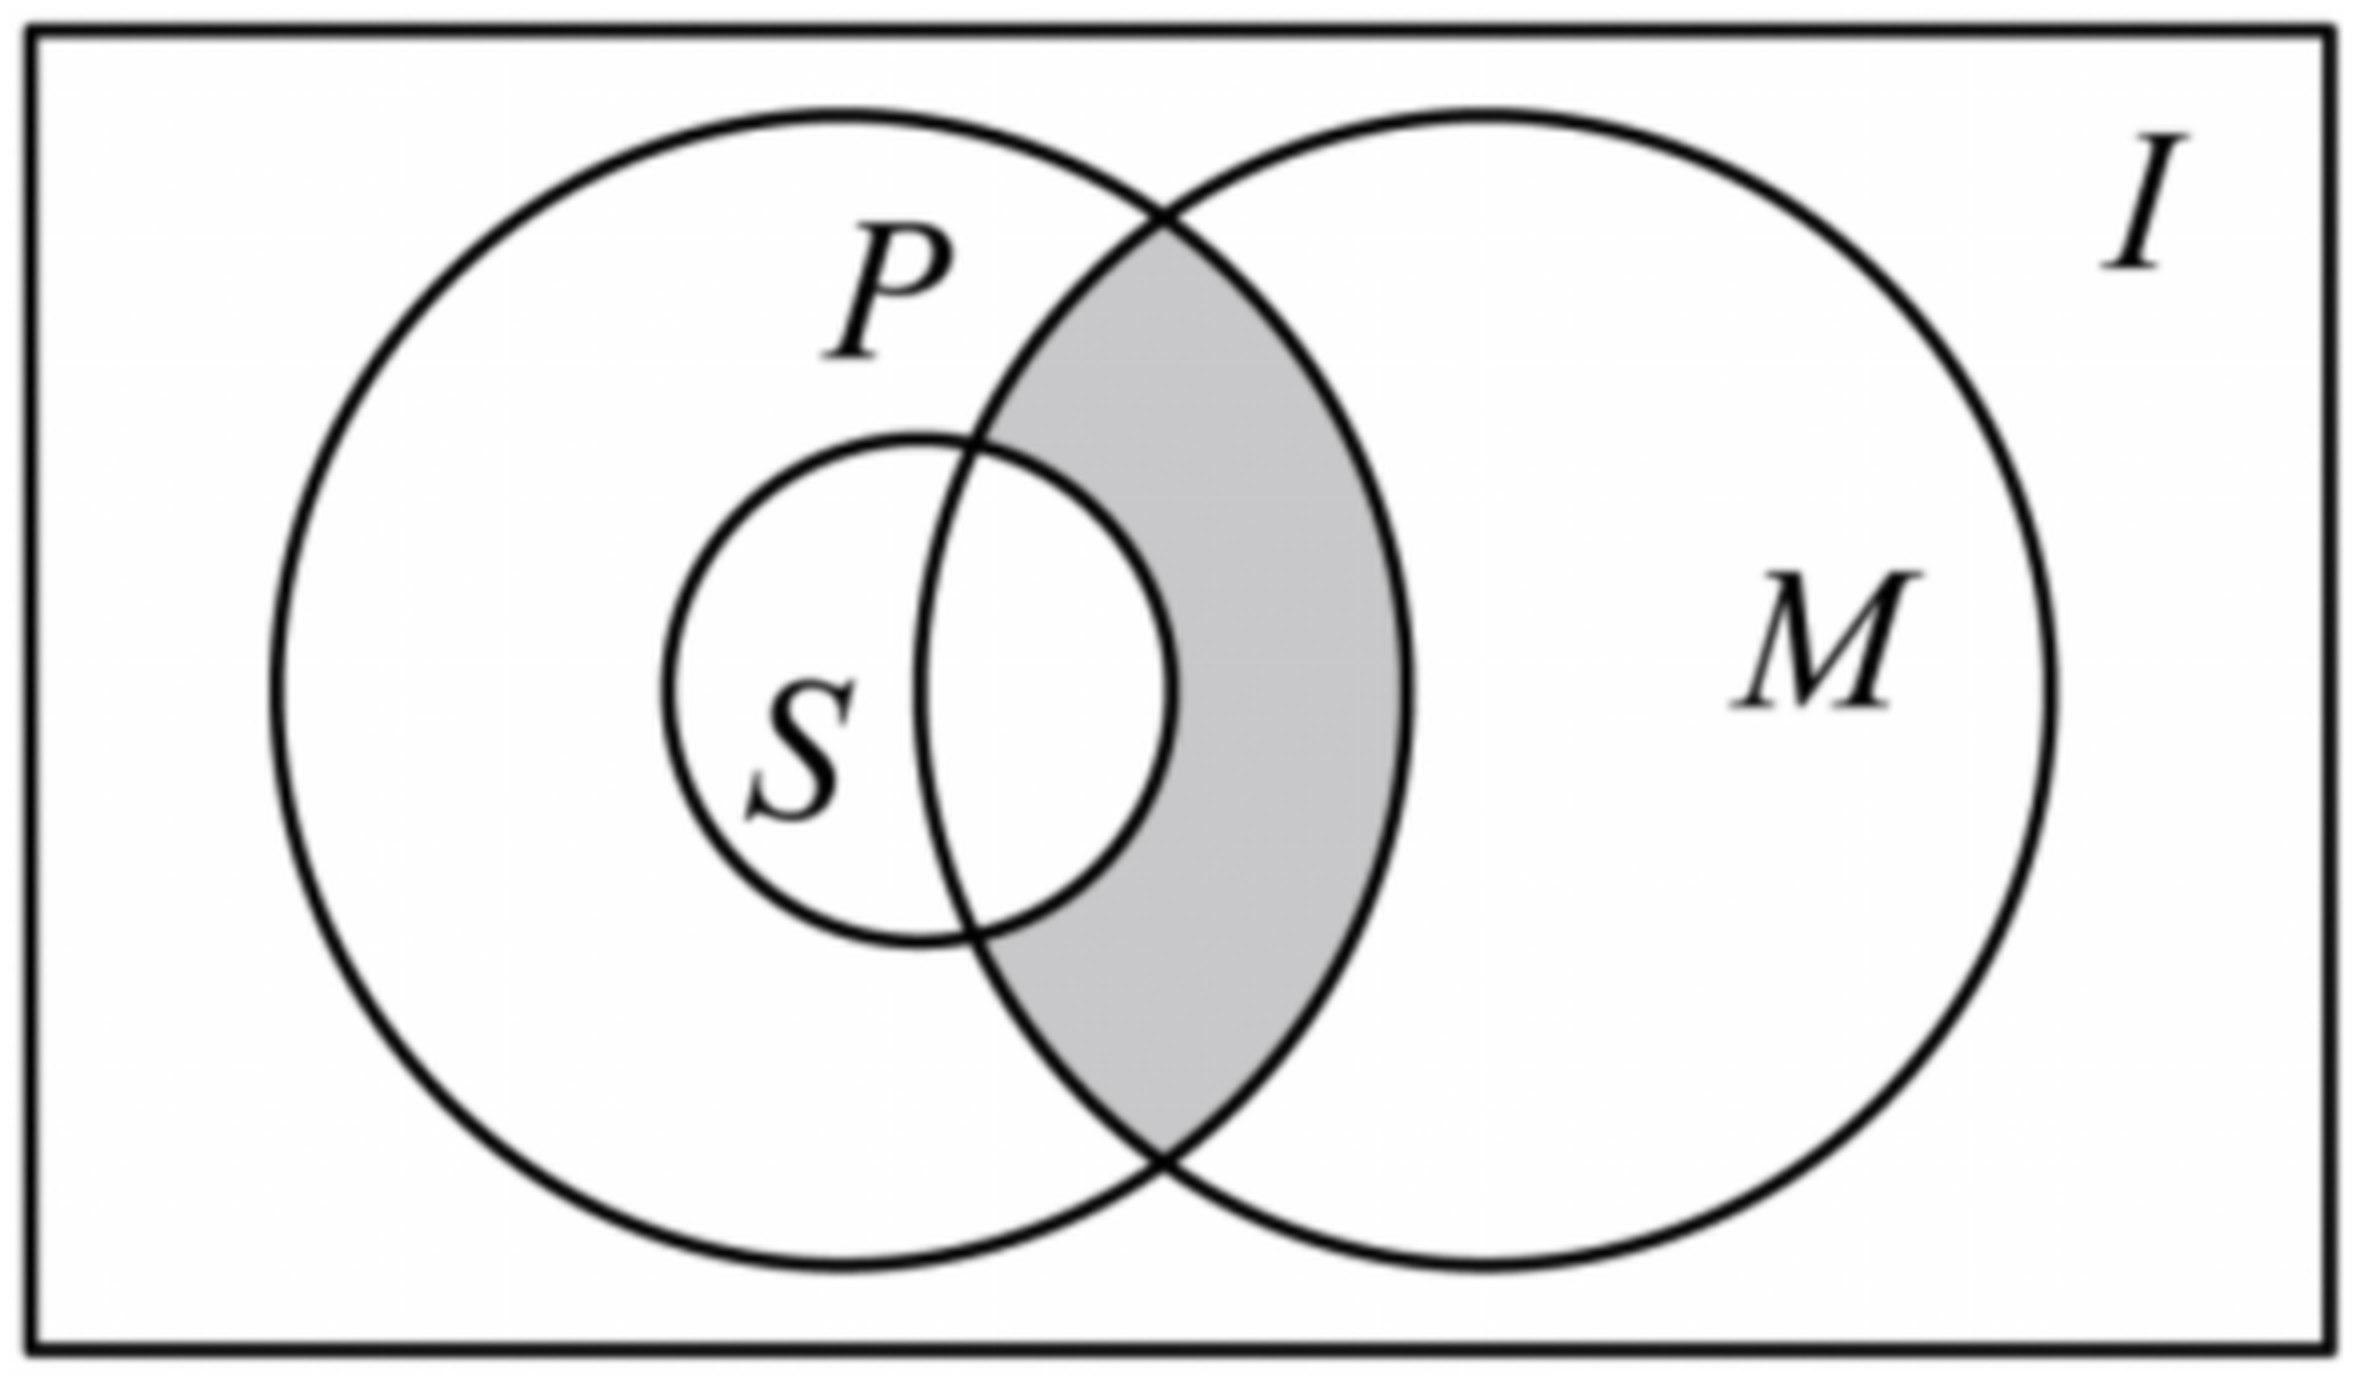
\includegraphics[width=0.46\textwidth]{figures/venn_MP_minus_S_h32.png}
\end{center}

\keepwithprev
A. $(M\cap P)\cap S$\qquad\qquad B. $(M\cap P)\cup S$

C. $(M\cap P)\cap\overline{S}$\qquad\qquad D. $(M\cap P)\cup\overline{S}$

\ans{$C$}

\ifanswer
\solbegin
\step{由 Venn 图得，集合表示 $M$、$P$ 的交集与 $S$ 的补集的交集，}
\step{即阴影部分所表示的集合是 $(M\cap P)\cap\overline{S}$. 故选 $C$.}
\solend

\fi

\item 若实数 $a$、$b$ 满足 $ab>0$，$a+2b=6$，则下列结论中错误的是\mbox{（\quad）}

\keepwithprev
A. $ab\leqslant\dfrac92$\qquad\qquad B. $a^2+4b^2\geqslant18$

C. $\dfrac1a+\dfrac2b$ 的最小值为 $\dfrac94$\qquad\qquad
D. $\dfrac{a^2}{a+1}+\dfrac{4b^2}{2b+1}$ 的最小值为 $\dfrac92$

\ans{$C$}

\ifanswer
\solbegin
\step{因为 $ab>0$，所以 $a$、$b$ 同号，又 $a+2b=6$，所以 $a$、$b$ 同正.}
\step{对于 $A$，由 $6=a+2b\geqslant2\sqrt{a\cdot2b}$ 得 $ab\leqslant\dfrac92$，故 $A$ 正确；}
\step{对于 $B$，由不等式 $\sqrt{\dfrac{m^2+n^2}2}\geqslant\dfrac{m+n}2$ 得
$\sqrt{\dfrac{a^2+(2b)^2}2}\geqslant\dfrac{a+2b}2=3$，}
\step{所以 $a^2+4b^2\geqslant18$，当且仅当 $a=2b=3$ 时取等号，故 $B$ 正确；}
\step{对于 $C$，$\dfrac1a+\dfrac2b
=\dfrac16\left(\dfrac1a+\dfrac2b\right)(a+2b)
=\dfrac16\left(5+\dfrac{2b}a+\dfrac{2a}b\right)$}
\step{$=\dfrac56+\dfrac13\left(\dfrac ba+\dfrac ab\right)
\geqslant\dfrac56+\dfrac13\times2\sqrt{\dfrac ba\cdot\dfrac ab}=\dfrac32$，}
\step{当且仅当 $\dfrac ba=\dfrac ab$，即 $a=b=2$ 时取等号，故 $C$ 错误；}
\step{对于 $D$，$\dfrac{a^2}{a+1}+\dfrac{4b^2}{2b+1}
=\dfrac{(a+1)^2-2(a+1)+1}{a+1}+\dfrac{(2b+1)^2-2(2b+1)+1}{2b+1}$}
\step{$=(a+1)-2+\dfrac1{a+1}+(2b+1)-2+\dfrac1{2b+1}
=(a+2b-2)+\dfrac1{a+1}+\dfrac1{2b+1}$}
\step{$=(6-2)+\dfrac{a+2b+2}{(a+1)(2b+1)}
=4+\dfrac8{(a+1)(2b+1)}$，}
\step{因为 $(a+1)(2b+1)\leqslant\left(\dfrac{a+1+2b+1}2\right)^2
=\left(\dfrac82\right)^2=16$，}
\step{当且仅当 $a+1=2b+1$，即 $a=2b=3$ 时取等号，}
\step{所以 $4+\dfrac8{(a+1)(2b+1)}\geqslant4+\dfrac8{16}=\dfrac92$，
故 $D$ 正确，其他几种方法同 12 题.}
\step{故选 $C$.}
\solend

\fi

% 注：本题的答案「D」原卷直接印在题干末尾的括号内，本稿按全稿惯例另提为 \ans{}。
\item 已知函数 $f(x)=x^2-2ax+a^2-1$，定义集合 $A=\{x\mid f(x)<0\}$. 若集合
$\{x\mid f(x)\in A\}=\varnothing$，则实数 $a$ 的取值范围是\mbox{（\quad）}

\keepwithprev
A. $(-3,-2)$\qquad B. $[-3,-2]$\qquad
C. $(-\infty,2)$\qquad D. $(-\infty,-2]$

\ans{$D$}

\item 非空集合 $A$ 具有如下性质：①若 $x$、$y\in A$，则 $\dfrac xy\in A$；
②若 $x$、$y\in A$，则 $x+y\in A$；

由此可知：下列判断中，错误的是\mbox{（\quad）}

\keepwithprev
A. $-1\notin A$\qquad\qquad B. $\dfrac{2025}{2026}\in A$

C. 若 $x$、$y\in A$，则 $xy\in A$\qquad\qquad
D. 若 $x$、$y\in A$，则 $x-y\in A$

\ans{$D$}

\ifanswer
\solbegin
\step{由题意得 $0\notin A$，$1\in A$，}
\step{对于 $A$，假设 $-1\in A$，则 $-1+1=0\in A$，矛盾，所以 $-1\notin A$，故 $A$ 正确；}
\step{对于 $B$，由 $1\in A$，得 $1+1=2\in A$，$2+1=3\in A$，…，$2025\in A$，$2026\in A$，}
\step{所以 $\dfrac{2025}{2026}\in A$，故 $B$ 正确；}
\step{对于 $C$，因为 $1\in A$，$x\in A$，所以 $\dfrac1x\in A$，
又因为 $y\in A$，所以 $\dfrac y{\frac1x}=xy\in A$，}
\step{故 $C$ 正确；}
\step{对于 $D$，因为 $1\in A$，$2\in A$，若 $x=1$，$y=2$，则 $x-y=-1\notin A$，故 $D$ 错误.}
\step{故选 $D$.}
\solend

\fi

\end{enumerate}

\bigsec{三、解答题}

\begin{enumerate}
\setcounter{enumi}{16}

\item 求下列关于实数 $x$ 的不等式的解集.

\begin{enumerate}[label=(\arabic*)]
\item $|2x+1|<5x-1$；
\item $\dfrac{(x-1)(x-3)(x-6)}{(x-2)(x-4)^2(x-5)}\geqslant0$.
\end{enumerate}

\ifanswer
\solbegin
\stepm{(1)}{因为不等式 $|2x+1|<5x-1$ 可化为 $-(5x-1)<2x+1<5x-1$，且 $5x-1>0$，}
\step{解得 $x>\dfrac23$，所以原不等式的解集为 $\left(\dfrac23,+\infty\right)$；}
\stepm{(2)}{不等式 $\dfrac{(x-1)(x-3)(x-6)}{(x-2)(x-4)^2(x-5)}\geqslant0$，}
\step{等价于 $(x-1)(x-3)(x-6)(x-2)(x-5)\geqslant0$，
且 $x-2\neq0$，$x-4\neq0$，$x-5\neq0$，}
\step{由“穿针引线法”，解得 $1\leqslant x<2$ 或 $3\leqslant x<4$ 或 $4<x<5$ 或 $x\geqslant6$，}
\step{所以不等式的解集为 $[1,2)\cup[3,4)\cup(4,5)\cup[6,+\infty)$.}
\solend

\fi

\ansspace[6]

\item 已知集合 $A=\left\{x\left|mx^2-mx+\dfrac{5m}2-6=0\right.\right\}\neq\varnothing$，
集合 $B=\{x\mid1<x<4$ 且 $x\in\Z\}$，$C=\{x\mid ax+3>0\}$；若 $A\cap B=A$.

\begin{enumerate}[label=(\arabic*)]
\item 求 $m$ 的取值范围.
\item 设 $m$ 的取值集合为 $D$，若 $C\cap D=\varnothing$，求 $m$ 的值及其对应 $a$ 的取值范围.
\end{enumerate}

\ans{略}

\ansspace[8]

\item 已知函数 $f(x)=x^2+(m-2)x+2m-1$.

\begin{enumerate}[label=(\arabic*)]
\item 若 $f(x)=0$ 的两根为 $x_1$、$x_2$，且 $|x_1-x_2|=2$，求实数 $m$ 的值；
\item 若函数 $y=f(x)$ 的图像在区间 $(0,1)$ 上与 $x$ 轴只有一个交点，
求实数 $m$ 的取值范围.
\end{enumerate}

\ifanswer
\solbegin
\stepm{(1)}{由题意得 $x_1+x_2=-(m-2)=2-m$，$x_1x_2=2m-1$，}
\step{由 $|x_1-x_2|=\sqrt{(x_1+x_2)^2-4x_1x_2}
=\sqrt{(2-m)^2-4(2m-1)}=2$，}
\step{化简得 $m^2-12m+4=0$，解得 $m=6\pm4\sqrt2$，故 $m=6\pm4\sqrt2$.}
\stepm{(2)}{当 $f(x)=0$ 只有一个根，且此根位于区间 $(0,1)$，}
\step{则 $\begin{cases}0<\dfrac{2-m}2<1\\[4pt]
\Delta=(m-2)^2-4(2m-1)=0\end{cases}$，
解得 $\begin{cases}0<m<2\\ m=6-2\sqrt7\text{ 或 }m=6+2\sqrt7\end{cases}$，}
\step{所以 $m=6-2\sqrt7$；}
\step{当 $f(x)=0$ 有两个根时，有一个根在区间 $(0,1)$ 内，且另一个根位于 $[0,1]$ 之外，}
\step{则 $\begin{cases}f(0)f(1)<0\\ \Delta=(m-2)^2-4(2m-1)>0\end{cases}$，
解得 $\begin{cases}\dfrac12<m<\dfrac23\\[4pt]
m<6-2\sqrt7\text{ 或 }m>6+2\sqrt7\end{cases}$，}
% 注：下一行原卷作「即 $\dfrac12<m<\dfrac32$」，按上一行方程组应为
%     $\dfrac12<m<\dfrac23$（同页最终答案也印证），照录未改，见文件头「原卷存疑」①。
\step{即 $\dfrac12<m<\dfrac32$；}
\step{当 $f(x)=0$ 有两个根位于区间 $[0,1]$ 内，且只有一个根在区间 $(0,1)$ 内，}
\step{则另一个根为 $0$ 时，得 $m=\dfrac12$，此时 $x_1+x_2=\dfrac32$，
解得另一个根 $x_2=\dfrac32>0$，故此种情况不符题意；}
\step{当 $f(x)=0$ 有两个根位于区间 $(0,1]$ 内，且只有一个根在区间 $(0,1)$ 内，}
\step{则另一个根为 $1$ 时，得 $m=\dfrac23$，此时 $x_1+x_2=\dfrac43$，
解得另一个根 $x_2=\dfrac13$，故此种情况符合题意；}
\step{综上所述，$m$ 的取值范围为
$\left(\dfrac12,\dfrac23\right]\cup\{6-2\sqrt7\}$.}
\solend

\fi

\ansspace[8]

\item 设集合 $A=\{a_1,a_2,a_3,a_4\}$，$B=\{b_1,b_2,b_3,b_4\}$，$C=\{2,3,4,6\}$，
新定义：集合 $A$ 中所有含 $k$ 个元素的子集中 $k$ 个元素之和组成的集合为“$k$ 元集和集”，
集合 $A$ 中所有含 $k$ 个元素的子集中最大元素减去剩余所有元素的和组成的集合为“$k$ 元差集”.

\begin{enumerate}[label=(\arabic*)]
\item 若 $A$ 的“$k$ 元集和集”为 $C$，求：集合 $A$.
\item 在 (1) 的条件下，若 $B$ 的“$k$ 元差集”为 $C$，求：所有满足条件的 $A\cap B$ 的真子集
个数之和.
\item 设 $b_1=a_1^2$，$b_2=a_2^2$，$b_3=a_3^2$，$b_4=a_4^2$，若 $A\cap B$ 为 $2$ 元集且
元素之和为 $10$ 且 $A$ 的“$2$ 元集和集”中最大元素不超过 $14$，求：所有满足条件的 $A$ 的
“$3$ 元差集”.
\end{enumerate}

\ifanswer
\solbegin
\stepm{(1)}{若 $A$ 的“$k$ 元集和集”为 $C$，$C=\{2,3,4,6\}$，则集合为 $\{-1,1,2,3\}$；}
\stepm{(2)}{$B$ 集合为 $\{5,3,0,-1\}$ 或 $\{9,3,1,0\}$ 或 $\{6,3,1,-1\}$，}
\step{故所有 $A\cap B$ 的真子集个数之和为 $13$；}
\stepm{(3)}{$b_1=a_1^2$，$b_2=a_2^2$，$b_3=a_3^2$，$b_4=a_4^2$，}
\step{若 $A\cap B$ 为 $2$ 元集且元素之和为 $10$，
且 $A$ 的“$2$ 元集和集”中最大元素不超过 $14$，}
% 注：下一行答案的第二个集合 $\{0,4,5,6\}$ 是 4 元集，而题问的却是「3 元差集」，
%     原卷如此，照录未改，见文件头「原卷存疑」③。
\step{则满足条件的 $A$ 的“$3$ 元差集” $\{1,3,5\}$ 或 $\{0,4,5,6\}$ 或 $\{2,4,5,8\}$.}
\solend

\fi

\ansspace[8]

\item 已知有限集 $X$、$Y$，定义集合 $X-Y=\{x\mid x\in X$ 且 $x\notin Y\}$，
$|X|$ 表示集合 $X$ 元素个数.

\begin{enumerate}[label=(\arabic*)]
\item 若 $X=\{1,2,3,4\}$，$Y=\{3,4,5\}$，写出集合 $X-Y$ 和 $Y-X$，以及
$|(X-Y)\cup(Y-X)|$ 的值；
\item 给定正整数 $n$，集合 $S=\{1,2,\cdots,n\}$，对于实数集的非空有限子集 $A$、$B$，
定义集合 $C=\{x\mid x=a+b,a\in A,b\in B\}$；

①求证：$|A-S|+|B-S|+|S-C|\geqslant1$；

②求 $|(A-S)\cup(S-A)|+|(B-S)\cup(S-B)|+|(C-S)\cup(S-C)|$ 的最小值.
\end{enumerate}

\ifanswer
\solbegin
\stepm{(1)}{由定义直接得 $X-Y=\{1,2\}$，$Y-X=\{5\}$，
$|(X-Y)\cup(Y-X)|=3$.}
% 注：下一句原卷作「显然 $|X|\geqslant0$」（按后文论证疑为 $|S|\geqslant0$），
%     照录未改，见文件头「原卷存疑」②。
\stepm{(2)}{①显然 $|X|\geqslant0$.}
\step{若 $A\cup B$ 中含有一个不在 $S$ 中的元素，则 $|A-S|+|B-S|\geqslant1$，
即 $|A-S|+|B-S|+|S-C|\geqslant1$.}
\step{若 $A\sub S$，且 $B\sub S$，则 $|A-S|=|B-S|=0$；}
\step{此时 $A$ 中最小的元素 $a\geqslant1$，$B$ 中最小的元素 $b\geqslant1$，
所以 $C$ 中最小的元素 $a+b\geqslant2$，所以 $1\notin C$.}
\step{因为 $S=\{1,2,\cdots,n\}$，所以 $|S-C|\geqslant1$，
即 $|A-S|+|B-S|+|S-C|\geqslant1$.}
\step{综上，$|A-S|+|B-S|+|S-C|\geqslant1$.}
\step{②由①得 $|A-S|+|B-S|+|S-C|\geqslant1$.}
\step{所以 $|(A-S)\cup(S-A)|+|(B-S)\cup(S-B)|+|(C-S)\cup(S-C)|$}
\step{$=|A-S|+|S-A|+|B-S|+|S-B|+|C-S|+|S-C|$}
\step{$\geqslant|S-A|+|S-B|+|C-S|+1$.}
\step{若 $A\cap S=\varnothing$，或 $B\cap S=\varnothing$，则 $|S-A|+|S-B|\geqslant n$.}
\step{若 $A\cap S\neq\varnothing$，且 $B\cap S\neq\varnothing$，
设 $A\cap S=\{a_1,a_2,\cdots,a_s\}$，$B\cap S=\{b_1,b_2,\cdots,b_t\}$，}
\step{且 $1\leqslant a_1<a_2<\cdots<a_s\leqslant n$，
$1\leqslant b_1<b_2<\cdots<b_t\leqslant n$，则 $|S-A|=n-s$，$|B-S|=n-t$.}
% 注：原卷的解析到此为止（第 10 页末），②的最小值并未给出，照录未补，
%     见文件头「原卷存疑」④。
\solend

\fi

\ansspace*[10]

\end{enumerate}

\end{document}
"
%
% 原始材料是微信公众号图文（公众号「魔都数学加油站」连载「27学年高一 32」，2026-09-25 发布，
% 原文标题「27学年高一32——2026-2027年上海市华师大二附中高一上周末作业4」），
% 正文为 10 张 PNG 页。**同一篇里各页分辨率不一致**（2560×3620 与 4762×6735 两档混排），
% 取 mmbiz.qpic.cn/<hash>/0 的原图档。原文本身就是一份**讲评版**——有的题下方印【解析】、
% 有的印【答案】，第 15 题的答案直接印在题干末尾的括号里。
% 试题文字、答案与解析均照原卷录入，未改内容。卷面的粉色斜水印属水印，未录入。
%
% ⚠ 卷首年份：本卷卷面印作「**2025-2026 年**」，与连载「27学年高一32」及公众号原文标题的
%   「2026-2027 年」**不一致**。经三人次分别把标题行裁出放大（4×—10×）独立判读，三次都读作
%   2025-2026，且校名作「华师大二附中」（无「东」字）、卷面亦无「上海市」三字。
%   按全稿「标题行照原卷」的口径，本稿照卷面排作「2025--2026 年…」——这是全稿唯一一份
%   年份不是 2026--2027 的卷子（其余 35 份均为 2026--2027）。
%
% 卷首标题：原卷印作「……年华师大二附中高一上周末作业 4」（公众号标题里的「上海市」
% 三字卷面标题行没有，本稿照卷面），年份区间按全稿惯例排 en dash，前缀照原卷保留「年」。
%
% 与原卷的排版差异（均已在 README「说明」中交代）：
%   ① 原文自**第 3 题**起（第 1、2 题未在该文中发布），故本稿题号亦自 3 起；
%   ② 原卷本就印有「一、填空题」「二、选择题」「三、解答题」三节标题，本稿照原卷分节，
%      只把标题改排成全稿统一的「大节标题」样式；
%   ③ 原卷第 6、8、9 题只印【答案】行（第 18 题的【答案】印作「略”），其余各题印【解析】，
%      第 15 题的答案直接印在题干末尾的括号内；本稿统一改为试卷版隐去、
%      答案版以 \ans{}／\ifanswer 块给出，两版彻底分离；
%   ④ 子集符号原卷两种并用：第 21(2)① 的 $A\sub S$、$B\sub S$ 带下划线，
%      第 3、10 题的 $(0,2)\subset(-\infty,3)$、$A\subset B$、$\overline{B}\subset\overline{A}$
%      作真包含，本稿分别照录为 $\sub$ 与 $\subset$；
%   ⑤ 补集符号原卷一律作上横线（$\overline{A}$、$\overline{B}$、$\overline{S}$），本稿照录；
%      空集原卷作「斜杠伸出圆外」的 $\varnothing$；
%   ⑥ 判别式记号原卷两种：第 4 题作粗体的 $\Delta$、第 11 题作细等宽的 $\triangle$，本稿照录；
%   ⑦ 数集记号原卷作斜体的 $R$、$Z$（第 4、18 题），本稿按全稿惯例统一写作 $\R$、$\Z$；
%   ⑧ 原卷填空的横线约两个字宽，本稿按全稿惯例统一排 \blankline[4.4em]；
%   ⑨ 原卷未印副标题，本稿按全稿惯例补出副标题「集合与常用逻辑用语」；
%   ⑩ 本卷只有第 13 题一图（韦恩图），原卷印在题干右侧，本稿移至题干之后；
%      图取原卷截图、4× LANCZOS 放大（figures/venn_MP_minus_S_h32.png）。
%
% 原卷存疑四处（均照抄原卷、未改，见源码中该处上方注释）：
%   ① 第 19(2)【解析】有「即 $\dfrac12<m<\dfrac32$」，按上一行的方程组应为
%      $\dfrac12<m<\dfrac23$（同页最终答案 $\left(\dfrac12,\dfrac23\right]$ 也印证）；
%   ② 第 21(2)① 首句作「显然 $|X|\geqslant0$」（按后文论证疑为 $|S|\geqslant0$）；
%   ③ 第 20(3) 的答案第二个集合 $\{0,4,5,6\}$ 是 4 元集，而题问的是「3 元差集」；
%   ④ 第 21(2)② 的解析**原卷就未写完**（第 10 页到「则 $|S-A|=n-s$，$|B-S|=n-t$」即止）。

\documentclass[a4paper,11pt]{article}
\usepackage{common}

\begin{document}

\examtitlest[3]{2025--2026 年华师大二附中高一上周末作业 4}{集合与常用逻辑用语}

\bigsec{一、填空题}

\begin{enumerate}
\setcounter{enumi}{2}

\item 设 $x$ 为实数，则“$x<3$”是“$x(x-2)<0$”的 \blankline[4.4em] 条件.

\ifanswer
\solbegin
\step{$x(x-2)<0$，解得 $0<x<2$，$(0,2)\subset(-\infty,3)$，}
\step{若 $x$ 属于“$x(x-2)<0$”，则属于“$x<3$”一定成立，即满足必要性，}
\step{若 $x$ 属于“$x<3$”，不一定满足“$x(x-2)<0$”，如 $x=-1$，即充分性不成立；}
\step{故“$x<3$”是“$x(x-2)<0$”的必要不充分条件.}
\solend

\fi

\item 若关于 $x$ 的不等式 $kx^2-kx+1>0$ 的解集为 $\R$，则实数 $k$ 的取值范围为
\blankline[4.4em].

\ifanswer
\solbegin
\step{①当 $k=0$ 时，不等式为 $1>0$ 恒成立，满足题意；}
\step{②当 $k\neq0$ 时，只要 $\begin{cases}k>0\\ \Delta=k^2-4k<0\end{cases}$，
解得 $0<k<4$；}
\step{所以不等式 $kx^2-kx+1>0$ 的解集为 $\R$，则实数 $k$ 的取值范围为 $[0,4)$.}
\solend

\fi

\item 已知 $1<a<3$，$-5<b<-2$，则 $\dfrac ab$ 的取值范围是 \blankline[4.4em].

\ifanswer
\solbegin
\step{因为 $-5<b<-2$，所以 $2<-b<5$，$\dfrac15<-\dfrac1b<\dfrac12$，又 $1<a<3$，}
\step{得 $\dfrac15<-\dfrac ab<\dfrac32$，则 $-\dfrac32<\dfrac ab<-\dfrac15$，
故 $\dfrac ab$ 的取值范围是 $\left(-\dfrac32,-\dfrac15\right)$.}
\solend

\fi

\item 关于 $x$ 的不等式 $\dfrac{ax-1}{x-a}>1$ 的解集为 $A$，且 $3\notin A$，
则实数 $a$ 的取值范围为 \blankline[4.4em].

\ans{$(-\infty,1]\cup[3,+\infty)$}

\item 若关于 $x$ 的不等式 $a\leqslant\dfrac34x^2-3x+4\leqslant b$ 的解集恰好是 $[a,b]$，
则 $b-a=$ \blankline[4.4em].

\ifanswer
\solbegin
\step{令 $f(x)=\dfrac34x^2-3x+4$，则 $f(x)$ 的对称轴为 $x=2$，}
\step{画出函数 $f(x)=\dfrac34x^2-3x+4=\dfrac34(x-2)^2+1$ 的图象，
得 $f(x)_{\min}=f(2)=1$，}
\step{由题意得 $a\leqslant1$，且 $f(a)=f(b)=b$，$a<b$，}
\step{由 $f(b)=b$ 得 $\dfrac34b^2-3b+4=b$，解得 $b=\dfrac43$（舍去）或 $b=4$，得 $b=4$，}
\step{由抛物线的对称轴为 $x=2$ 得 $a=0$，所以 $b-a=4$.}
\solend

\fi

\item 若关于 $x$ 的方程 $x^2-2kx+k+4=0$ 在 $[1,2]$ 上有解，则实数 $k$ 的取值范围为
\blankline[4.4em].

\ans{$\left[\dfrac83,5\right]$}

\item 记关于 $x$ 的方程 $x^2-2mx-2m+3=0$ 的两实根为 $x_1$、$x_2$，
则 $(x_1-2)^2+(x_2-2)^2$ 的最小值为 \blankline[4.4em].

\ans{$2$}

\item 若“$|mx^2-4x+3|\geqslant2$”的必要非充分条件是“$x\leqslant1$ 或 $x\geqslant4$”，
则实数 $m$ 的取值范围是 \blankline[4.4em].

\ifanswer
\solbegin
\step{记 $|mx^2-4x+3|\geqslant2$ 的解集为集合 $A$，
$B=\{x\mid x\leqslant1\text{ 或 }x\geqslant4\}$，}
\step{则 $\overline{A}$ 为 $|mx^2-4x+3|<2$ 的解集，$\overline{B}=\{x\mid1<x<4\}$；}
\step{因为 $B$ 是 $A$ 的必要非充分条件，所以 $A\subset B$，
得 $\overline{B}\subset\overline{A}$，}
\step{即对任意 $x\in(1,4)$，都有 $|mx^2-4x+3|<2$ 恒成立.}
\step{因为 $|mx^2-4x+3|<2$，$1<x<4$，所以 $-2<mx^2-4x+3<2$，}
\step{化简得
$-5\left(\dfrac1x\right)^2+4\left(\dfrac1x\right)
<m<-\left(\dfrac1x\right)^2+4\left(\dfrac1x\right)$；}
\step{令 $t=\dfrac1x$，$g(t)=-5t^2+4t$，$h(t)=-t^2+4t$，
且 $t\in\left(\dfrac14,1\right)$；}
\step{所以 $g(t)=-5t^2+4t=-5\left(t-\dfrac25\right)^2+\dfrac45$，
当 $t=\dfrac25$ 时，$g(t)$ 取得最大值 $\dfrac45$，}
\step{$h(t)=-t^2+4t=-(t-2)^2+4$，当 $t=\dfrac14$ 时，$h(t)$ 取得最小值，
即 $h(t)>h\left(\dfrac14\right)=\dfrac{15}{16}$；}
\step{因为对任意 $t\in\left(\dfrac14,1\right)$，$g(t)<m<h(t)$ 恒成立，
所以 $g\left(\dfrac25\right)<m\leqslant h\left(\dfrac14\right)$，}
\step{即 $\dfrac45<m\leqslant\dfrac{15}{16}$，
所以 $m$ 的取值范围是 $\left(\dfrac45,\dfrac{15}{16}\right]$.}
\solend

\fi

\item 已知关于 $x$ 的方程 $x^2+2(m-2)x+m^2-3m+3=0$ 有两个不相等的实数根 $x_1$、$x_2$，则

$\dfrac{mx_1}{x_1-1}+\dfrac{mx_2}{x_2-1}-\dfrac2{x_1+x_2-2}$ 的最大值为 \blankline[4.4em].

\ifanswer
\solbegin
\step{关于 $x$ 的方程 $x^2+2(m-2)x+m^2-3m+3=0$ 有两个不相等的实数根 $x_1$、$x_2$，}
\step{则 $\triangle=4(m-2)^2-4(m^2-3m+3)=-4m+4>0$，得 $m<1$，}
\step{且 $x_1+x_2=-2(m-2)$，$x_1x_2=m^2-3m+3$，}
\step{$\dfrac{mx_1}{x_1-1}+\dfrac{mx_2}{x_2-1}-\dfrac2{x_1+x_2-2}
=\dfrac{m[2x_1x_2-(x_1+x_2)]}{x_1x_2-(x_1+x_2)+1}+\dfrac1{m-1}$}
\step{$=\dfrac{2m(m-1)^2}{m^2-m}+\dfrac1{m-1}=2(m-1)+\dfrac1{m-1}$，}
\step{又因为 $m<1$，所以 $m-1<0$，则 $1-m>0$，}
\step{所以 $2(1-m)+\dfrac1{1-m}\geqslant2\sqrt{2(1-m)\cdot\dfrac1{1-m}}=2\sqrt2$，}
\step{当且仅当 $2(1-m)=\dfrac1{1-m}$ 时，即 $m=1-\dfrac{\sqrt2}2$ 时取等号，}
\step{所以 $2(m-1)+\dfrac1{m-1}\leqslant-2\sqrt2$，
即 $\dfrac{mx_1}{x_1-1}+\dfrac{mx_2}{x_2-1}-\dfrac2{x_1+x_2-2}$ 的最大值为 $-2\sqrt2$.}
\solend

\fi

\item 若正实数 $a$、$b$ 满足 $a+2b=ab$，则 $\dfrac4{a^2+2a}+\dfrac1{2b^2+b}$ 的最小值是
\blankline[4.4em].

\ifanswer
\solbegin
\stepm{法一}{由 $a+2b=ab$，得 $\dfrac2a+\dfrac1b=1$，}
\step{令 $x=\dfrac1a$，$y=\dfrac1b$，则 $x$、$y>0$，$2x+y=1$，$2x+1+y+2=4$，}
\step{所以 $\dfrac4{a^2+2a}+\dfrac1{2b^2+b}
=\dfrac4{\frac1{x^2}+\frac2x}+\dfrac1{\frac2{y^2}+\frac1y}
=\dfrac{4x^2}{2x+1}+\dfrac{y^2}{y+2}$（*）}
\step{$=\dfrac{(2x+1)^2-2(2x+1)+1}{2x+1}+\dfrac{(y+2)^2-4(y+2)+4}{y+2}$}
\step{$=2x-1+\dfrac1{2x+1}+y-2+\dfrac4{y+2}=\dfrac1{2x+1}+\dfrac4{y+2}-2$}
\step{$=\dfrac14\left(\dfrac1{2x+1}+\dfrac4{y+2}\right)(2x+1+y+2)-2$}
\step{$=\dfrac14\left[5+\dfrac{y+2}{2x+1}+\dfrac{4(2x+1)}{y+2}\right]-2
\geqslant\dfrac14(5+2\sqrt4)-2=\dfrac14$，}
\step{当且仅当 $\dfrac{y+2}{2x+1}=\dfrac{4(2x+1)}{y+2}$，
即 $x=\dfrac16$，$y=\dfrac23$ 时取等号，}
\step{故 $\dfrac4{a^2+2a}+\dfrac1{2b^2+b}$ 的最小值是 $\dfrac14$.}
\stepm{法二}{在法一（*）后，由权方和不等式，得
$\dfrac4{a^2+2a}+\dfrac1{2b^2+b}
=\dfrac{4x^2}{2x+1}+\dfrac{y^2}{y+2}
\geqslant\dfrac{(2x+y)^2}{2x+1+y+2}=\dfrac14$，}
\step{当且仅当……，故 $\dfrac4{a^2+2a}+\dfrac1{2b^2+b}$ 的最小值是 $\dfrac14$.}
\stepm{法三}{注意到
$\left(\dfrac{a+2}a+\dfrac{2b+1}b\right)\left(\dfrac4{a^2+2a}+\dfrac1{2b^2+b}\right)$}
\step{$\geqslant
\left(\sqrt{\dfrac{a+2}a\cdot\dfrac4{a^2+2a}}
+\sqrt{\dfrac{2b+1}b\cdot\dfrac1{2b^2+b}}\right)^2
=\left(\dfrac2a+\dfrac1b\right)^2$，}
\step{其中 $\dfrac{a+2}a+\dfrac{2b+1}b=3+\dfrac{a+2b}{ab}=4$，
$\dfrac2a+\dfrac1b=\dfrac{a+2b}{ab}=1$，}
\step{所以 $\dfrac4{a^2+2a}+\dfrac1{2b^2+b}\geqslant\dfrac14$，
当且仅当……，故 $\dfrac4{a^2+2a}+\dfrac1{2b^2+b}$ 的最小值是 $\dfrac14$.}
\solend

\fi

\end{enumerate}

\bigsec{二、选择题}

\begin{enumerate}
\setcounter{enumi}{12}

\item 如图，$I$ 为全集，$M$、$P$、$S$ 是 $I$ 的三个子集，则阴影部分所表示的集合是
\mbox{（\quad）}

\begin{center}
% 图取原卷截图、4× LANCZOS 放大（原卷把图印在题干右侧，本稿移至此处，见文件头⑩）。
% 矩形为全集 $I$，左大圆 $P$（内下方含小圆 $S$，其右侧伸入 $P$ 与 $M$ 的重叠区）、
% 右大圆 $M$；阴影是 $P$、$M$ 重叠的透镜形区域挖掉 $S$ 后剩下的部分（左缘呈弯月形）。
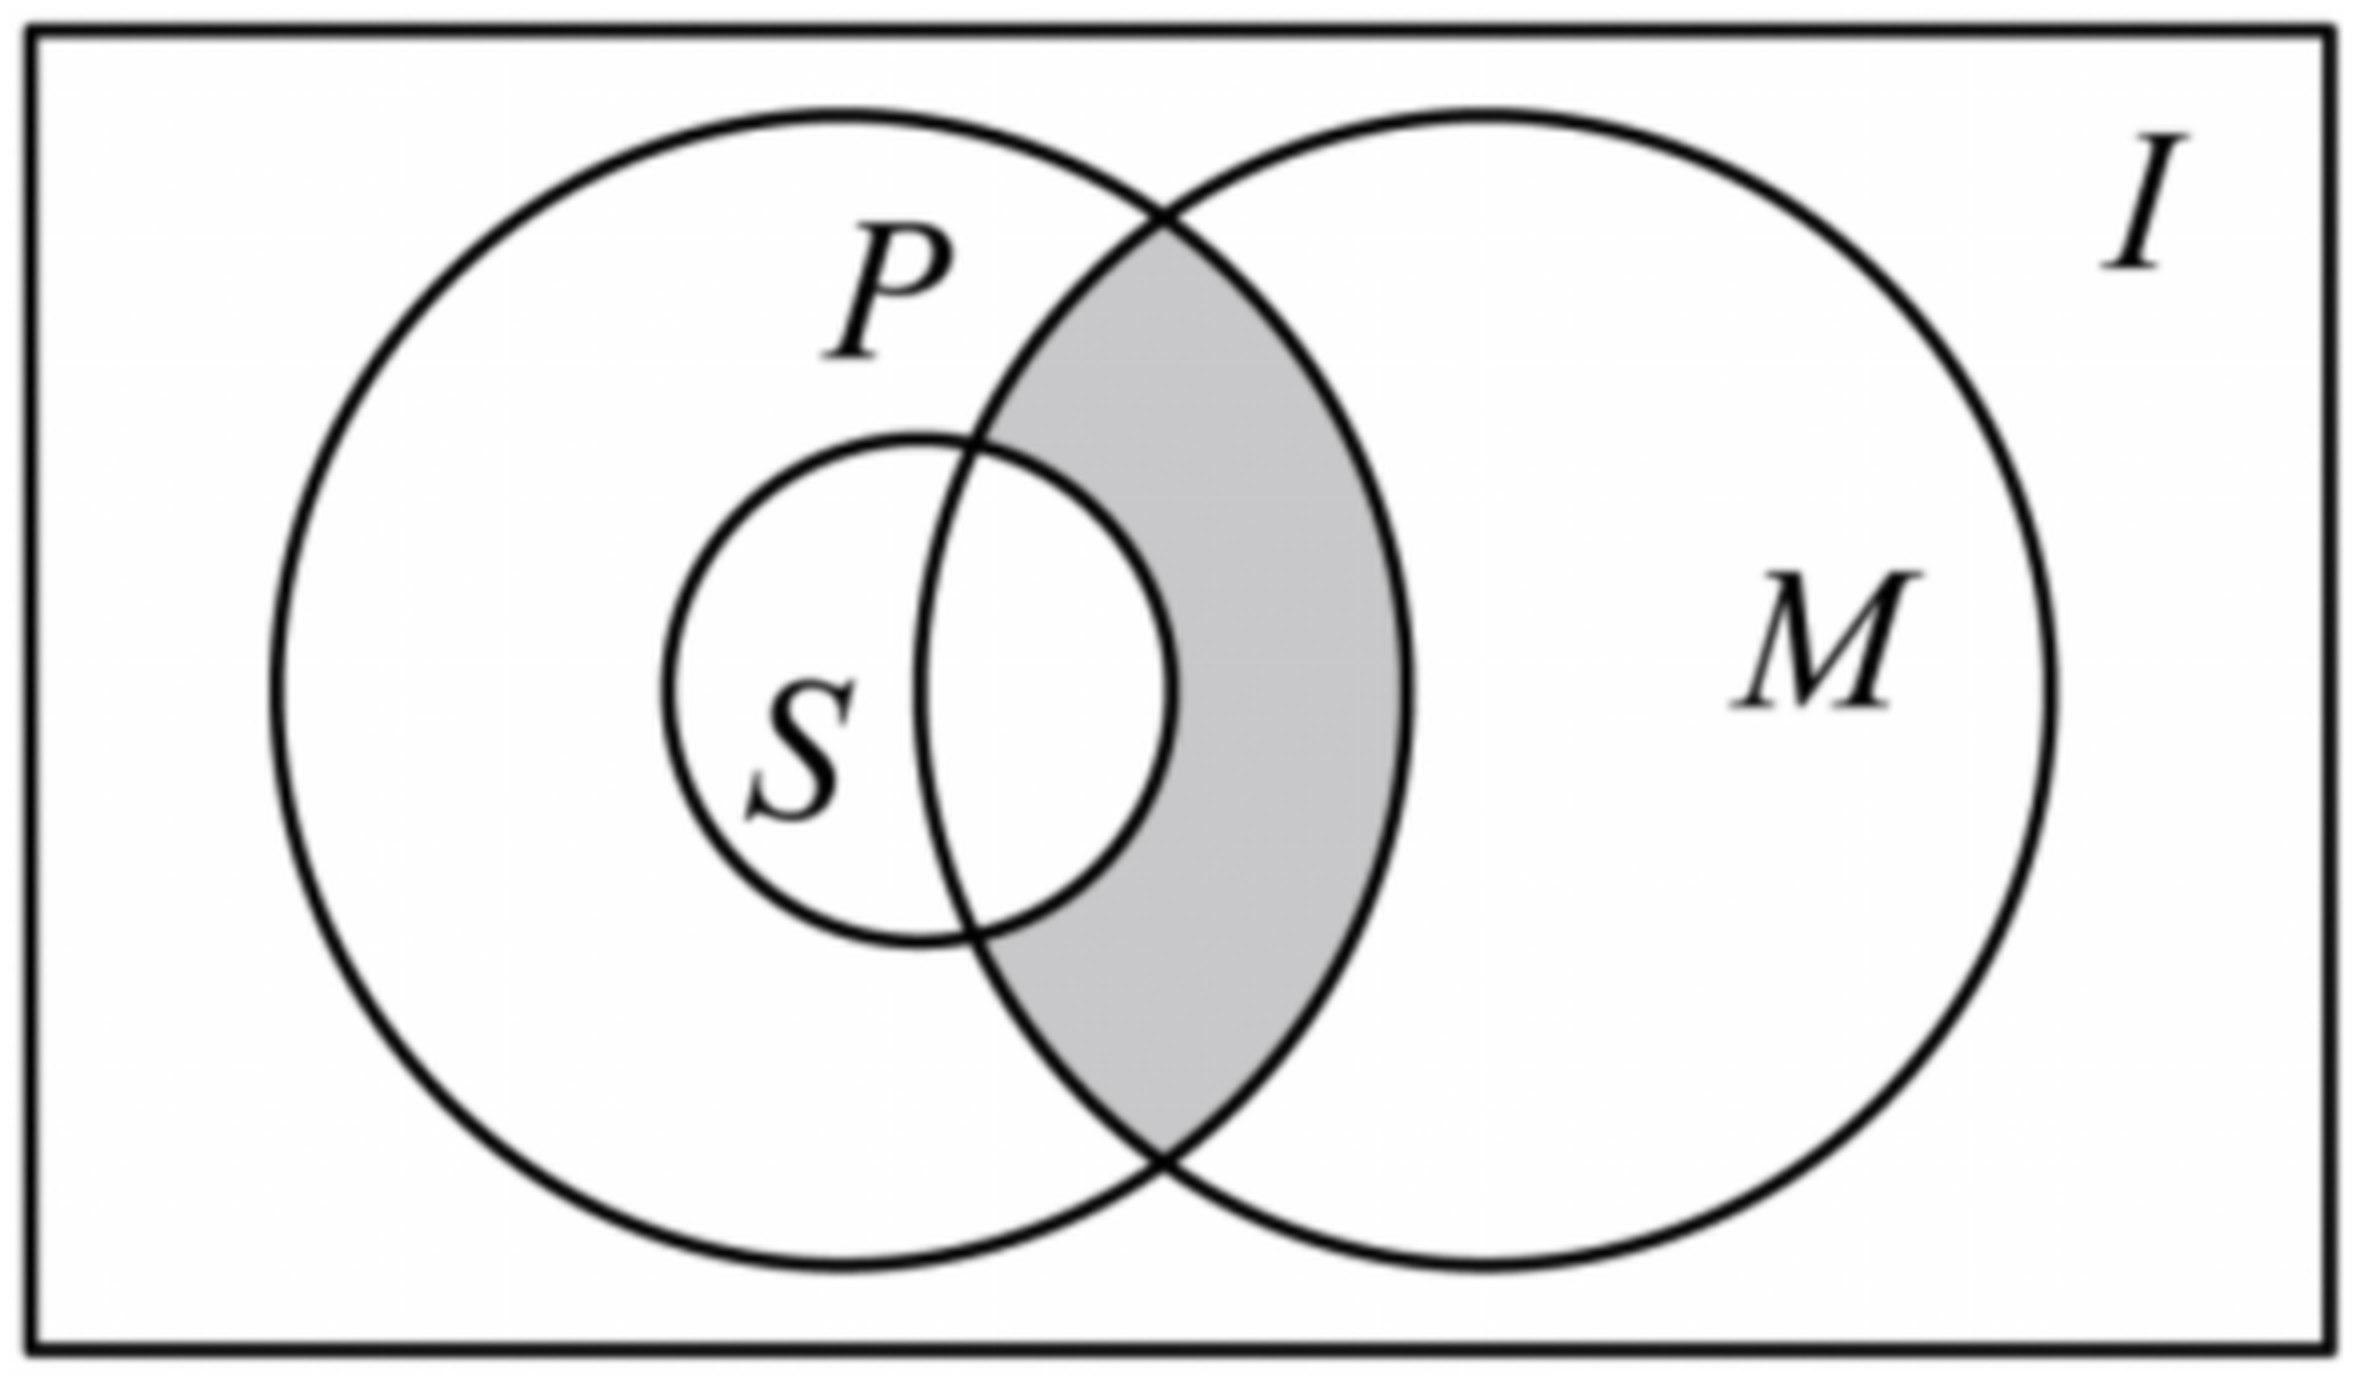
\includegraphics[width=0.46\textwidth]{figures/venn_MP_minus_S_h32.png}
\end{center}

\keepwithprev
A. $(M\cap P)\cap S$\qquad\qquad B. $(M\cap P)\cup S$

C. $(M\cap P)\cap\overline{S}$\qquad\qquad D. $(M\cap P)\cup\overline{S}$

\ans{$C$}

\ifanswer
\solbegin
\step{由 Venn 图得，集合表示 $M$、$P$ 的交集与 $S$ 的补集的交集，}
\step{即阴影部分所表示的集合是 $(M\cap P)\cap\overline{S}$. 故选 $C$.}
\solend

\fi

\item 若实数 $a$、$b$ 满足 $ab>0$，$a+2b=6$，则下列结论中错误的是\mbox{（\quad）}

\keepwithprev
A. $ab\leqslant\dfrac92$\qquad\qquad B. $a^2+4b^2\geqslant18$

C. $\dfrac1a+\dfrac2b$ 的最小值为 $\dfrac94$\qquad\qquad
D. $\dfrac{a^2}{a+1}+\dfrac{4b^2}{2b+1}$ 的最小值为 $\dfrac92$

\ans{$C$}

\ifanswer
\solbegin
\step{因为 $ab>0$，所以 $a$、$b$ 同号，又 $a+2b=6$，所以 $a$、$b$ 同正.}
\step{对于 $A$，由 $6=a+2b\geqslant2\sqrt{a\cdot2b}$ 得 $ab\leqslant\dfrac92$，故 $A$ 正确；}
\step{对于 $B$，由不等式 $\sqrt{\dfrac{m^2+n^2}2}\geqslant\dfrac{m+n}2$ 得
$\sqrt{\dfrac{a^2+(2b)^2}2}\geqslant\dfrac{a+2b}2=3$，}
\step{所以 $a^2+4b^2\geqslant18$，当且仅当 $a=2b=3$ 时取等号，故 $B$ 正确；}
\step{对于 $C$，$\dfrac1a+\dfrac2b
=\dfrac16\left(\dfrac1a+\dfrac2b\right)(a+2b)
=\dfrac16\left(5+\dfrac{2b}a+\dfrac{2a}b\right)$}
\step{$=\dfrac56+\dfrac13\left(\dfrac ba+\dfrac ab\right)
\geqslant\dfrac56+\dfrac13\times2\sqrt{\dfrac ba\cdot\dfrac ab}=\dfrac32$，}
\step{当且仅当 $\dfrac ba=\dfrac ab$，即 $a=b=2$ 时取等号，故 $C$ 错误；}
\step{对于 $D$，$\dfrac{a^2}{a+1}+\dfrac{4b^2}{2b+1}
=\dfrac{(a+1)^2-2(a+1)+1}{a+1}+\dfrac{(2b+1)^2-2(2b+1)+1}{2b+1}$}
\step{$=(a+1)-2+\dfrac1{a+1}+(2b+1)-2+\dfrac1{2b+1}
=(a+2b-2)+\dfrac1{a+1}+\dfrac1{2b+1}$}
\step{$=(6-2)+\dfrac{a+2b+2}{(a+1)(2b+1)}
=4+\dfrac8{(a+1)(2b+1)}$，}
\step{因为 $(a+1)(2b+1)\leqslant\left(\dfrac{a+1+2b+1}2\right)^2
=\left(\dfrac82\right)^2=16$，}
\step{当且仅当 $a+1=2b+1$，即 $a=2b=3$ 时取等号，}
\step{所以 $4+\dfrac8{(a+1)(2b+1)}\geqslant4+\dfrac8{16}=\dfrac92$，
故 $D$ 正确，其他几种方法同 12 题.}
\step{故选 $C$.}
\solend

\fi

% 注：本题的答案「D」原卷直接印在题干末尾的括号内，本稿按全稿惯例另提为 \ans{}。
\item 已知函数 $f(x)=x^2-2ax+a^2-1$，定义集合 $A=\{x\mid f(x)<0\}$. 若集合
$\{x\mid f(x)\in A\}=\varnothing$，则实数 $a$ 的取值范围是\mbox{（\quad）}

\keepwithprev
A. $(-3,-2)$\qquad B. $[-3,-2]$\qquad
C. $(-\infty,2)$\qquad D. $(-\infty,-2]$

\ans{$D$}

\item 非空集合 $A$ 具有如下性质：①若 $x$、$y\in A$，则 $\dfrac xy\in A$；
②若 $x$、$y\in A$，则 $x+y\in A$；

由此可知：下列判断中，错误的是\mbox{（\quad）}

\keepwithprev
A. $-1\notin A$\qquad\qquad B. $\dfrac{2025}{2026}\in A$

C. 若 $x$、$y\in A$，则 $xy\in A$\qquad\qquad
D. 若 $x$、$y\in A$，则 $x-y\in A$

\ans{$D$}

\ifanswer
\solbegin
\step{由题意得 $0\notin A$，$1\in A$，}
\step{对于 $A$，假设 $-1\in A$，则 $-1+1=0\in A$，矛盾，所以 $-1\notin A$，故 $A$ 正确；}
\step{对于 $B$，由 $1\in A$，得 $1+1=2\in A$，$2+1=3\in A$，…，$2025\in A$，$2026\in A$，}
\step{所以 $\dfrac{2025}{2026}\in A$，故 $B$ 正确；}
\step{对于 $C$，因为 $1\in A$，$x\in A$，所以 $\dfrac1x\in A$，
又因为 $y\in A$，所以 $\dfrac y{\frac1x}=xy\in A$，}
\step{故 $C$ 正确；}
\step{对于 $D$，因为 $1\in A$，$2\in A$，若 $x=1$，$y=2$，则 $x-y=-1\notin A$，故 $D$ 错误.}
\step{故选 $D$.}
\solend

\fi

\end{enumerate}

\bigsec{三、解答题}

\begin{enumerate}
\setcounter{enumi}{16}

\item 求下列关于实数 $x$ 的不等式的解集.

\begin{enumerate}[label=(\arabic*)]
\item $|2x+1|<5x-1$；
\item $\dfrac{(x-1)(x-3)(x-6)}{(x-2)(x-4)^2(x-5)}\geqslant0$.
\end{enumerate}

\ifanswer
\solbegin
\stepm{(1)}{因为不等式 $|2x+1|<5x-1$ 可化为 $-(5x-1)<2x+1<5x-1$，且 $5x-1>0$，}
\step{解得 $x>\dfrac23$，所以原不等式的解集为 $\left(\dfrac23,+\infty\right)$；}
\stepm{(2)}{不等式 $\dfrac{(x-1)(x-3)(x-6)}{(x-2)(x-4)^2(x-5)}\geqslant0$，}
\step{等价于 $(x-1)(x-3)(x-6)(x-2)(x-5)\geqslant0$，
且 $x-2\neq0$，$x-4\neq0$，$x-5\neq0$，}
\step{由“穿针引线法”，解得 $1\leqslant x<2$ 或 $3\leqslant x<4$ 或 $4<x<5$ 或 $x\geqslant6$，}
\step{所以不等式的解集为 $[1,2)\cup[3,4)\cup(4,5)\cup[6,+\infty)$.}
\solend

\fi

\ansspace[6]

\item 已知集合 $A=\left\{x\left|mx^2-mx+\dfrac{5m}2-6=0\right.\right\}\neq\varnothing$，
集合 $B=\{x\mid1<x<4$ 且 $x\in\Z\}$，$C=\{x\mid ax+3>0\}$；若 $A\cap B=A$.

\begin{enumerate}[label=(\arabic*)]
\item 求 $m$ 的取值范围.
\item 设 $m$ 的取值集合为 $D$，若 $C\cap D=\varnothing$，求 $m$ 的值及其对应 $a$ 的取值范围.
\end{enumerate}

\ans{略}

\ansspace[8]

\item 已知函数 $f(x)=x^2+(m-2)x+2m-1$.

\begin{enumerate}[label=(\arabic*)]
\item 若 $f(x)=0$ 的两根为 $x_1$、$x_2$，且 $|x_1-x_2|=2$，求实数 $m$ 的值；
\item 若函数 $y=f(x)$ 的图像在区间 $(0,1)$ 上与 $x$ 轴只有一个交点，
求实数 $m$ 的取值范围.
\end{enumerate}

\ifanswer
\solbegin
\stepm{(1)}{由题意得 $x_1+x_2=-(m-2)=2-m$，$x_1x_2=2m-1$，}
\step{由 $|x_1-x_2|=\sqrt{(x_1+x_2)^2-4x_1x_2}
=\sqrt{(2-m)^2-4(2m-1)}=2$，}
\step{化简得 $m^2-12m+4=0$，解得 $m=6\pm4\sqrt2$，故 $m=6\pm4\sqrt2$.}
\stepm{(2)}{当 $f(x)=0$ 只有一个根，且此根位于区间 $(0,1)$，}
\step{则 $\begin{cases}0<\dfrac{2-m}2<1\\[4pt]
\Delta=(m-2)^2-4(2m-1)=0\end{cases}$，
解得 $\begin{cases}0<m<2\\ m=6-2\sqrt7\text{ 或 }m=6+2\sqrt7\end{cases}$，}
\step{所以 $m=6-2\sqrt7$；}
\step{当 $f(x)=0$ 有两个根时，有一个根在区间 $(0,1)$ 内，且另一个根位于 $[0,1]$ 之外，}
\step{则 $\begin{cases}f(0)f(1)<0\\ \Delta=(m-2)^2-4(2m-1)>0\end{cases}$，
解得 $\begin{cases}\dfrac12<m<\dfrac23\\[4pt]
m<6-2\sqrt7\text{ 或 }m>6+2\sqrt7\end{cases}$，}
% 注：下一行原卷作「即 $\dfrac12<m<\dfrac32$」，按上一行方程组应为
%     $\dfrac12<m<\dfrac23$（同页最终答案也印证），照录未改，见文件头「原卷存疑」①。
\step{即 $\dfrac12<m<\dfrac32$；}
\step{当 $f(x)=0$ 有两个根位于区间 $[0,1]$ 内，且只有一个根在区间 $(0,1)$ 内，}
\step{则另一个根为 $0$ 时，得 $m=\dfrac12$，此时 $x_1+x_2=\dfrac32$，
解得另一个根 $x_2=\dfrac32>0$，故此种情况不符题意；}
\step{当 $f(x)=0$ 有两个根位于区间 $(0,1]$ 内，且只有一个根在区间 $(0,1)$ 内，}
\step{则另一个根为 $1$ 时，得 $m=\dfrac23$，此时 $x_1+x_2=\dfrac43$，
解得另一个根 $x_2=\dfrac13$，故此种情况符合题意；}
\step{综上所述，$m$ 的取值范围为
$\left(\dfrac12,\dfrac23\right]\cup\{6-2\sqrt7\}$.}
\solend

\fi

\ansspace[8]

\item 设集合 $A=\{a_1,a_2,a_3,a_4\}$，$B=\{b_1,b_2,b_3,b_4\}$，$C=\{2,3,4,6\}$，
新定义：集合 $A$ 中所有含 $k$ 个元素的子集中 $k$ 个元素之和组成的集合为“$k$ 元集和集”，
集合 $A$ 中所有含 $k$ 个元素的子集中最大元素减去剩余所有元素的和组成的集合为“$k$ 元差集”.

\begin{enumerate}[label=(\arabic*)]
\item 若 $A$ 的“$k$ 元集和集”为 $C$，求：集合 $A$.
\item 在 (1) 的条件下，若 $B$ 的“$k$ 元差集”为 $C$，求：所有满足条件的 $A\cap B$ 的真子集
个数之和.
\item 设 $b_1=a_1^2$，$b_2=a_2^2$，$b_3=a_3^2$，$b_4=a_4^2$，若 $A\cap B$ 为 $2$ 元集且
元素之和为 $10$ 且 $A$ 的“$2$ 元集和集”中最大元素不超过 $14$，求：所有满足条件的 $A$ 的
“$3$ 元差集”.
\end{enumerate}

\ifanswer
\solbegin
\stepm{(1)}{若 $A$ 的“$k$ 元集和集”为 $C$，$C=\{2,3,4,6\}$，则集合为 $\{-1,1,2,3\}$；}
\stepm{(2)}{$B$ 集合为 $\{5,3,0,-1\}$ 或 $\{9,3,1,0\}$ 或 $\{6,3,1,-1\}$，}
\step{故所有 $A\cap B$ 的真子集个数之和为 $13$；}
\stepm{(3)}{$b_1=a_1^2$，$b_2=a_2^2$，$b_3=a_3^2$，$b_4=a_4^2$，}
\step{若 $A\cap B$ 为 $2$ 元集且元素之和为 $10$，
且 $A$ 的“$2$ 元集和集”中最大元素不超过 $14$，}
% 注：下一行答案的第二个集合 $\{0,4,5,6\}$ 是 4 元集，而题问的却是「3 元差集」，
%     原卷如此，照录未改，见文件头「原卷存疑」③。
\step{则满足条件的 $A$ 的“$3$ 元差集” $\{1,3,5\}$ 或 $\{0,4,5,6\}$ 或 $\{2,4,5,8\}$.}
\solend

\fi

\ansspace[8]

\item 已知有限集 $X$、$Y$，定义集合 $X-Y=\{x\mid x\in X$ 且 $x\notin Y\}$，
$|X|$ 表示集合 $X$ 元素个数.

\begin{enumerate}[label=(\arabic*)]
\item 若 $X=\{1,2,3,4\}$，$Y=\{3,4,5\}$，写出集合 $X-Y$ 和 $Y-X$，以及
$|(X-Y)\cup(Y-X)|$ 的值；
\item 给定正整数 $n$，集合 $S=\{1,2,\cdots,n\}$，对于实数集的非空有限子集 $A$、$B$，
定义集合 $C=\{x\mid x=a+b,a\in A,b\in B\}$；

①求证：$|A-S|+|B-S|+|S-C|\geqslant1$；

②求 $|(A-S)\cup(S-A)|+|(B-S)\cup(S-B)|+|(C-S)\cup(S-C)|$ 的最小值.
\end{enumerate}

\ifanswer
\solbegin
\stepm{(1)}{由定义直接得 $X-Y=\{1,2\}$，$Y-X=\{5\}$，
$|(X-Y)\cup(Y-X)|=3$.}
% 注：下一句原卷作「显然 $|X|\geqslant0$」（按后文论证疑为 $|S|\geqslant0$），
%     照录未改，见文件头「原卷存疑」②。
\stepm{(2)}{①显然 $|X|\geqslant0$.}
\step{若 $A\cup B$ 中含有一个不在 $S$ 中的元素，则 $|A-S|+|B-S|\geqslant1$，
即 $|A-S|+|B-S|+|S-C|\geqslant1$.}
\step{若 $A\sub S$，且 $B\sub S$，则 $|A-S|=|B-S|=0$；}
\step{此时 $A$ 中最小的元素 $a\geqslant1$，$B$ 中最小的元素 $b\geqslant1$，
所以 $C$ 中最小的元素 $a+b\geqslant2$，所以 $1\notin C$.}
\step{因为 $S=\{1,2,\cdots,n\}$，所以 $|S-C|\geqslant1$，
即 $|A-S|+|B-S|+|S-C|\geqslant1$.}
\step{综上，$|A-S|+|B-S|+|S-C|\geqslant1$.}
\step{②由①得 $|A-S|+|B-S|+|S-C|\geqslant1$.}
\step{所以 $|(A-S)\cup(S-A)|+|(B-S)\cup(S-B)|+|(C-S)\cup(S-C)|$}
\step{$=|A-S|+|S-A|+|B-S|+|S-B|+|C-S|+|S-C|$}
\step{$\geqslant|S-A|+|S-B|+|C-S|+1$.}
\step{若 $A\cap S=\varnothing$，或 $B\cap S=\varnothing$，则 $|S-A|+|S-B|\geqslant n$.}
\step{若 $A\cap S\neq\varnothing$，且 $B\cap S\neq\varnothing$，
设 $A\cap S=\{a_1,a_2,\cdots,a_s\}$，$B\cap S=\{b_1,b_2,\cdots,b_t\}$，}
\step{且 $1\leqslant a_1<a_2<\cdots<a_s\leqslant n$，
$1\leqslant b_1<b_2<\cdots<b_t\leqslant n$，则 $|S-A|=n-s$，$|B-S|=n-t$.}
% 注：原卷的解析到此为止（第 10 页末），②的最小值并未给出，照录未补，
%     见文件头「原卷存疑」④。
\solend

\fi

\ansspace*[10]

\end{enumerate}

\end{document}
